\documentclass[12pt, a4paper,twoside,titlepage]{book}
\usepackage[left=3.5cm,top=2cm,right=3cm,includehead]{geometry}


%% ¡¡ Modificar por el alumno !! %%
\newcommand{\grado}{Grado en Diseño y Desarrollo de Videojuegos}
\newcommand{\titulotrabajo}{Representación de las enfermedades mentales en videojuegos}
\newcommand{\curso}{Curso Académico 2021-2022}
\newcommand{\autor}{Andrea Rodríguez González}
\newcommand{\tutor}{Joaquín Arias Herrero}
\newcommand{\cotutor}{María Zapata Cáceres}



%%%%%%%%%%%%%%%%%%%%%%% Paquetes (no modificar)
\usepackage[utf8]{inputenc}
\usepackage[spanish,es-lcroman,es-tabla]{babel}
\usepackage[T1]{fontenc}
\usepackage[pdftex]{graphicx}
\usepackage{mathptmx}
\usepackage{amsmath}
\usepackage{amssymb}
\usepackage{enumitem}
\usepackage[Algoritmo]{algorithm}
\usepackage{algorithmic}
\usepackage[justification=centering]{caption}
\setlength\abovecaptionskip{0.5em}
\setlength\belowcaptionskip{-0.25em}
 \usepackage[figuresright]{rotating}
 \usepackage{booktabs}
\usepackage{multirow}
\usepackage{xltabular}
\usepackage{longtable}
\usepackage{pdflscape}
\usepackage{afterpage}
\usepackage{relsize}
\usepackage{color}
\usepackage{xcolor}
\usepackage{booktabs}
\usepackage{subcaption}
\definecolor{linkcolor}{RGB}{52,59,144}
\definecolor{Comment}  {RGB}{169,082,044}
\definecolor{Bluedark} {RGB}{0,0,180}
\definecolor{Bluelight}{RGB}{070,100,250}
\definecolor{Browndark}{rgb}{0.2,0.2,0.2}
\definecolor{gray}{rgb}{0.6,0.6,0.6}

%%%%%%%%%%%%%%%%%%%%%%% Estilo de bibliografia
\usepackage{csquotes}
\PassOptionsToPackage{
  natbib=true,
  style=bwl-FU,%	authoryear-comp,
  maxbibnames=99,
  firstinits=true,
  backend=bibtex,
}   {biblatex}
\usepackage{biblatex}
\DeclareNameAlias{sortname}{last-first} 
\bibliography{bibliografia.bib}

\DeclareCiteCommand{\cite}[\mkbibparens]
{\usebibmacro{prenote}}
{\usebibmacro{citeindex}%
  \printtext[bibhyperref]{\printnames[cite]{labelname} \printfield[cite]{year}}}%{\usebibmacro{cite}}}
{\multicitedelim}
{\usebibmacro{postnote}}
% Titles in bold
\DeclareFieldFormat*{title}{\textbf{#1}}

\DeclareCiteCommand{\citetitle}
{\usebibmacro{prenote}}
{\usebibmacro{citeindex}%
  \printtext[bibhyperref]{\printfield[cite]{labeltitle} (\printfield[cite]{year})}}
{\multicitedelim}
{\usebibmacro{postnote}}


%%%%%%%%%%%%%%%%%%%%%%% Estilo de enlaces

\usepackage[colorlinks=true,pdftex]{hyperref}
\hypersetup{
  linktocpage,
  bookmarksopen=true,
  bookmarksnumbered=true,
  breaklinks=true,
  hidelinks,
  pageanchor=true,
  colorlinks,
  linktocpage,
  citecolor=linkcolor,
  urlcolor=linkcolor,
  linkcolor=linkcolor
}
\renewcommand*{\UrlFont}{\ttfamily\small\relax}
    
%%%%%%%%%%%%%%%%%%%%%%% Estilo de páginas
\usepackage{fancyhdr}
\pagestyle{fancy}
\fancyhf{}
\setlength{\headheight}{15.2pt}
\renewcommand{\chaptermark}[1]{\markboth{\uppercase{#1}}{}}
\renewcommand*{\headrulewidth}{0pt}
\fancyhead[EL]{ \textsf{\relsize{-1}{\leftmark\ }} \hrulefill }
\fancyhead[OR]{ \hrulefill \textsf{\relsize{-1}{\ \nouppercase\rightmark} } }
\fancyfoot[C]{\thepage}

  
%%%%%%%%%%%%%%%%%%%%%%% Estilo de código
\usepackage{textcomp}
\usepackage{bold-extra}
\usepackage{listings}
\newcommand{\code}{\lstinline[
  language={},
  columns=fullflexible,
  basicstyle=\color{Browndark}]
}
\lstdefinestyle{Default}{
  basicstyle = \relsize{-1}\ttfamily\color{Bluelight},
  keywordstyle=\color{Bluedark},
  stringstyle=\color{Browndark},
  commentstyle = \color{Comment},
  numberstyle=\tiny\color{Bluedark},
  xleftmargin=0.5cm,
  numbers=left,
  basewidth = 0.48em,
  columns=fullflexible,
  breaklines,
  breakatwhitespace=true,
  moredelim=*[s][\color{Browndark}]{[}{]},
  moredelim=[s][\color{Bluedark}]{\{}{\}},
  mathescape = true,
  upquote = true,
  inputencoding=utf8,
  extendedchars=true,
  literate      =        % Support additional characters
  {á}{{\'a}}1  {é}{{\'e}}1  {í}{{\'i}}1 {ó}{{\'o}}1  {ú}{{\'u}}1
  {Á}{{\'A}}1  {É}{{\'E}}1  {Í}{{\'I}}1 {Ó}{{\'O}}1  {Ú}{{\'U}}1
  {ä}{{\"a}}1  {ë}{{\"e}}1  {ï}{{\"i}}1 {ö}{{\"o}}1  {ü}{{\"u}}1
  {ñ}{{\~n}}1  {Ñ}{{\~N}}1  {¿}{{?`}}1  {¡}{{!`}}1
  {\\\%}{{\textbackslash\%}}2  {~}{{\raisebox{0.5ex}{\texttildelow}}}1
}
\lstdefinestyle{Python}{style=Default, language=Python}
\lstdefinestyle{Unity}{style=Default, language=[Sharp]C}
\lstdefinestyle{Latex}{style=Default, language=[LaTeX]TeX}
%% Selecciona el estilo por defecto: Python, Unity, Latex, Default, ...
\lstset{style=Latex}


%%%%%%%%%%%%%%%%%%%%%%%%%%%%%%% Portada
\renewcommand*{\maketitle}{%
\begin{titlepage}
  \pagestyle{plain}

  \begin{center}
    \vspace*{-4em}
    
\includegraphics[scale=.9]{URJ_logo_Color_POS}\\
    \vspace*{4em}
    \textsc{\Large Escuela Técnica Superior de Ingeniería Informática}\\
    \vspace*{2em}
    \textsc{\Large \grado}\\  % Grado definido por el alumno
    \vspace*{3em}
     \textsc{\large \curso\\}  % Curso definido por el alumno
    \vspace*{1.5em}
    \textsc{\large Trabajo Fin de Grado\\}
    \vspace*{13em}
    \textbf{\LARGE \titulotrabajo\\}  % Titulo del TFG  definido por el alumno
    \vspace*{5em}
    {%
      \large
      \begin{tabular}{rl}
        \textbf{Autora:} & \textbf{\autor}\\[.5em]
        {Tutelado por:} & {\tutor}\\[-.25em]
                          & {\cotutor}\\
      \end{tabular}
    }
  \end{center}
  
\end{titlepage}
}

   
%%%%%%%%%%%%%%%%%%%%%%%%%%%%%%% Otros ajustes
\let\origdoublepage\cleardoublepage
\renewcommand{\cleardoublepage}{\clearpage{\pagestyle{empty}\origdoublepage}}

% Table dimensions
\setlength{\tabcolsep}{7.5pt} 
\def\arraystretch{1.25}

% Itemize spacing
\setlist{nolistsep, parsep=0.25em}

% Lines and paragraph
\setlength{\parindent}{0cm}
\setlength{\parskip}{1em}
\def\baselinestretch{1}


\sloppy

%%%%%%%%%%%%%%%%%%%%%%%%%%%%%%% Para Incluir Comentarios
\usepackage[
% disable,
textsize=footnotesize,color=red!20!white]{todonotes}
\reversemarginpar
\newcommand{\comm}[1]{\todo[linecolor=yellow]{\textsf{#1}}}
\newcommand{\commin}[1]{\todo[inline,linecolor=yellow]{\textsf{#1}}}


%%%%%%%%%%%%%%%%%%%%%%%%%%%%%%% Inicio del documento
\begin{document}
\maketitle



%%%%%%%%%%%%%%%%%%%%%%%%% FrontMatter
\cleardoublepage
\pagenumbering{roman}
\setcounter{page}{1}

\chapter*{Resumen}
\addcontentsline{toc}{chapter}{Resumen}

Los videojuegos son una de las industrias en mayor auge. Lo mismo ocurre, desgraciadamente, con las enfermedades mentales. Cada vez son más las personas que padecen trastornos mentales y sin embargo su representación en medios aún no es equiparable a la realidad. 

En este trabajo se ha realizado un estudio para comprobar el estado de la representación de enfermedades en videojuegos de diferentes épocas, analizando qué enfermedades se representan, de qué manera, quién los ha desarrollado, etc. Por otro lado, se ha estudiado a la población, tanto su conocimiento sobre videojuegos de esta temática, como las enfermedades mentales que estos padecen. Aunando ambos estudios, se ha llegado a la conclusión de que todavía falta representación, sobre todo de algunas enfermedades mentales y que esta representación debe desestigmatizarse. 

Por ello, se ha desarrollado un prototipo de un videojuego, llamado ``Insania'', en el que se puede experimentar, desde los ojos de tres personajes, cada uno los cuales padece una enfermedad de las menos representadas en videojuegos cómo es enfrentarse a ciertas situaciones padeciendo estas enfermedades. Los trastornos representados han sido el trastorno de la conducta alimentaria, el trastorno de ansiedad social y la depresión por la poca representación que hay de ellos y el alto porcentaje de afectados por ellos. De ese modo se quiere mostrar una nueva forma de representar este tipo de enfermedades y se anima al sector a que lo siga haciendo, pues es muy importante que haya visibilidad y normalidad. 


\noindent \textbf{Palabras clave}:
\begin{itemize}
   \item Videojuegos
   \item Unity
   \item Salud mental
   \item Trastornos mentales
\end{itemize}



\chapter*{Agradecimientos}
\addcontentsline{toc}{chapter}{Agradecimientos}



%%%%%%%%%%%%%%%%%%%%%%%%% Índices
{
  \setlength{\parskip}{1pt}

  % Índice de contenidos
  \cleardoublepage
  \phantomsection
  \addcontentsline{toc}{chapter}{\contentsname}
  \tableofcontents

  % Índice de tablas (OPCIONAL)
  \cleardoublepage
  \phantomsection
  \addcontentsline{toc}{chapter}{\noindent \listtablename}
  \listoftables

  % Índice de figuras (OPCIONAL)
  \cleardoublepage
  \phantomsection
  \addcontentsline{toc}{chapter}{\listfigurename}
  \listoffigures
}


%%%%%%%%%%%%%%%%%%%%%%%%%%%%%% MainMatter
\cleardoublepage
\pagenumbering{arabic}
\setcounter{page}{1}

\chapter{Introducción}


\section{Contexto y alcance}

Las enfermedades o trastornos mentales son uno de los mayores problemas de la sociedad actual. Van pasando los años y el aumento de conocimiento así como el avance de la medicina y la aparición de nuevas técnicas y tecnologías están facilitando y mejorando la salud física de todos nosotros, sin embargo aún no se presta la suficiente atención a la salud mental. Pese a que casi el 50\% de los adultos padezca un trastorno mental a lo largo de su vida, más de la mitad de ellos con una sintomatología moderada o grave, sólo un 20\% de estas personas reciben ayuda profesional \cite{articuloIntro1}. 

Poco a poco se está tratando de dar más visibilidad a estos problemas no tan perceptibles desde el exterior pero igual de afectantes e incapacitantes. Durante muchos años han sido estigmatizados y un motivo de burla o menosprecio. Todavía en la sociedad está mal visto llorar, hablar de los problemas claramente, no hay ningún tipo de enseñanza sobre la inteligencia emocional y usamos expresiones que mantienen la exclusión a personas que padecen estos trastornos.  

Estos trastornos o enfermedades mentales van desde la ansiedad y depresión, dos de las enfermedades mentales más frecuentes en la actualidad, a otras más desconocidas o estigmatizadas como pueden ser la esquizofrenia o trastornos disociativos. 

Uno de los motivos principales de que aún no se considere como un problema importante es la falta de información. Todo el mundo conoce los síntomas de un catarro, una gripe o una gastroenteritis, e incluso de enfermedades más erradicadas como puede ser la gota, que afecta, en función del país, de un 0,1 hasta un 10\% de la población \cite{articuloIntro2}. 

Sin embargo, mucha de la gente que conoce a una persona con pensamientos suicidas o que comete el suicidio, que actualmente es la primera causa de muerte entre los jóvenes en España \cite{fundacionSuicidio}, y suponen actualmente el doble de fallecimientos que los producidos en accidentes de tráfico, no ha sabido detectar que esa persona no se encontraba bien, no ha tenido información sobre cómo ayudarla o a quién recurrir, algunos incluso habrán despreciado algunos de los indicios. 

Mucha gente sufre a diario enfermedades mentales más silenciosas como la ansiedad y la depresión, que derivan en problemas físicos, en problemas sociales, laborales, educativos, y sin embargo sólo se pone el foco a lo que ocasiona, y no en a qué es debido. Hay quienes desconocen tener esas enfermedades por no saber ni que existen, mucho menos van a tratar de consultarlas con alguien, al considerar que es normal. 

Como comentaba Abelle en un vídeo del canal \citetitle{special} llamado ``Managing Schizophrenia as a New mom'', \cite{videoEsquizofrenia}, ella no supo que padecía esquizofrenia hasta los 25 años. Consideraba que las alucinaciones que tenía eran normales, pensaba que todo el mundo lo viviría también. Su madre también lo padecía de forma no medicada y por parte de su alrededor sólo recibía rechazo, sobre todo de pequeña, cuando el resto de niños la solían dejar sola. Cuando fue haciéndose mayor y comentando con sus amigos algunos de sus comportamientos y pensamientos paranoicos entendió que no era lo normal y acudió a un psiquiatra, que se lo diagnosticó y comenzó a probar diferentes medicaciones para tratarlo, algo que le cambió la vida. 

Igual que ella, existen cientos y miles de personas alrededor del mundo que conviven con enfermedades que les afectan a su vida diaria y que podrían tener tratamiento bien a base de terapia, de medicamentos, o una combinación de ambas, que no lo reciben por mero desconocimiento y por tener a las enfermedades mentales tan apartadas de la vida real, cuando forman parte del día a día de la mayoría.

Otra chica con ansiedad generalizada comentaba también en un vídeo del mismo canal de YouTube que cuando comunicó a su familia que lo padecía fue cuando se enteró que muchos otros miembros de su familia también lo habían padecido o seguían padeciéndolo y medicándose para ello. ``Once I started opening up apparently all of my family has it. I was like... 'Why did no one tell me this?' That would have made it so much easier for me to understand what I was going through in the beginning.'' \cite{videoTAG}. \textit{``Una vez me empecé a abrir, aparentemente toda mi familia lo tiene. Fue como... '¿Por qué nadie me había dicho esto?' Eso me lo habría puesto más fácil para entender por lo que estaba pasando en un principio''}. De haberlo sabido antes, podría haber sentido más compañía, podría haber buscado ayuda antes, podría saber que tenía predisposición a tenerlo, igual que se conocen otras tantas enfermedades que son hereditarias y se va haciendo un seguimiento de los descendientes.

Como se mencionará a lo largo del trabajo, en la sección \ref{sec:estadoArte}, en el videojuego \citetitle{hellblade17} consiguieron reflejar cómo es vivir con una enfermedad tan incapacitante y atormentante como puede ser la psicosis. Gracias a hacerlo con la ayuda de profesionales y enfermos, acabaron recibiendo mensajes de personas que se habían sentido muy identificadas y que les daban las gracias por haber podido representar y reflejar lo que toda la vida llevaban intentando hacer entender a su círculo cercano. Recibiendo mensajes como \textbf{\textit{'Your game made me cry because it showed me it was possible to undestand me'}} \textit{('Vuestro juego me hizo llorar porque me mostró que era posible entenderme')} o \textbf{\textit{'I had a psychotic break several years ago. My brother never understood. I overheard him say he was ashamed of me. After this game, he turned to me and said he was sorry. You got a message across that I never could'}} \textit{('Tuve un brote psicótico hace unos cuantos años. Mi hermano nunca lo entendió. Le escuché decir que estaba avergonzado de mí. Después de este juego, se volvió hacia mí y me pidió disculpas. Conseguísties mandar un mensaje que yo nunca pude')}. 

Como puede verse en estos mensajes, y en estas experiencias, se necesita visibilidad e información de que las enfermedades mentales existen, y de que existen de formas muy diversas entre todos nosotros. 

La industria del videojuego, por otro lado, es una industria que se encuentra actualmente en auge, teniendo un valor estimado en 2020 de 159.3 miles de millones de dolares, y una estimación para 2023 de alrededor de 200 miles de millones de dólares \cite{articuloIntroVideojuegos}. En cuanto al número de jugadores, se calcula que fue de 2.69 miles de millones en 2020 \cite{articuloIntroVideojuegos2}. 

Es una industria, por tanto, que llega a mucha gente. Generalmente además el público está formado por niños y personas jóvenes, que pueden adquirir de estos no solo entretenimiento y una forma de pasar el tiempo, sino también aprendizaje sobre ciertos aspectos de la vida. 

Por tanto, en una época en la que las enfermedades mentales aún están invisibilizadas y son tan comunes, utilizar los videojuegos para normalizarlas puede ser un punto clave para la sociedad. A diferencia de otros medios, como podrían ser los libros, series o películas, en un videojuego se participa de la historia, es más fácil empatizar, sentir lo que está sintiendo el protagonista o aprender de la 'convivencia virtual' con otros personajes que padezcan algún tipo de enfermedad para poder aplicarlo a la vida real. 

Muchos investigadores y científicos ya han remarcado los beneficios que puede suponer utilizar videojuegos tanto para tratar enfermedades mentales, como para visibilizarlas. Sin embargo, hacen hincapié en la necesidad de que sean los desarrolladores de videojuegos, quienes conocen la base de los videojuegos y saben hacerlos disfrutables y entretenidos, los que colaboren junto con gente especializada y experta, para producir videojuegos que puedan cambiar la vida de todos como sociedad, y, en concreto, de las personas que padecen estos trastornos o enfermedades \cite{articuloDesarrolloCient}.

A lo largo de este trabajo se mencionarán videojuegos que representan enfermedades mentales desarrollados por gente que las padece, tratando de mostrar al mundo su experiencia de forma que otros puedan sentirse identificados, y otros tantos aprender de ello, como ocurrió con el videojuego Hellblade Senua's Sacrifice. No por ello lo que se represente es aplicable a todas las personas con determinada enfermedad, pues cada persona vive su propia realidad, su propia sintomatología, etc., pero sí que puede ayudar a tener una visión más cercana de las enfermedades mentales y de las personas que las padecen. 

Hasta hace unos años, la mayoría de las representaciones de enfermedades mentales se veían en enemigos violentos y malvados, utilizando la enfermedad para justificar ese comportamiento, dando la imagen de que todos los enfermos lo tendrían también. Todavía a día de hoy nos encontramos con esas representaciones estigmatizadas y estereotipadas, no obstante, poco a poco se van viendo nuevas ideas donde se reflejan de diferentes formas, como se podrá ver en la sección \ref{sec:estadoArte}. 

Dada la importancia que tiene la representación de todo tipo de enfermedades mentales, se ha diseñado y desarrollado también un prototipo donde se representan varias enfermedades mentales, partiendo de la información recabada a lo largo de la investigación.

\chapter{Objetivos}


\section{Objetivos principales}

    Los objetivos principales de este trabajo son investigar y analizar cuál es la situación actual con respecto a los videojuegos y la representación que hacen de las enfermededades mentales, dado que a primera vista se considera insuficiente. Se comprobará también qué enfermedades suelen representarse y de qué forma. Además, se observará cómo ha ido variando a lo largo del tiempo esta representación.
    
    De ese modo se tendrá una base para realizar un prototipo de una experiencia jugable donde se apliquen los conocimientos obtenidos, se traten las enfermedades mentales menos representadas o que requieran más representación, y se mostrará una nueva forma de representar enfermedades mentales en videojuegos. En este caso, con una experiencia jugable que se centra en la enfermedad en sí.
    
   
    \section{Objetivos secundarios}
    
     Se analizará tanto el estado del arte de los videojuegos, en general, como la opinión de una serie de encuestados, para conocer la frecuencia con la que se conocen videojugeos que muestren enfermedades mentales y cómo se sienten con respecto a estas representaciones. Esto se podrá encontrar, tanto en la sección \ref{sec:estadoArte} como en la sección \ref{sec:encuestaVid}.       
       
     A raíz del análisis de la representación de las enfermedades mentales, se investigará también cómo puede afectar una mejor o peor representación para la sociedad. Aparte de esto, cómo pueden ayudar en general los videojuegos y qué puede hacerse para desarrollar videojuegos más correctos al tratar este tema.   
     
     Para el desarrollo del prototipo se realizará un diseño del videojuego, que se puede encontrar en la sección \ref{sec:diseño} tanto software como de las artes, diseñando los personajes su historia, motivo de su creación, trasfondo, etc. en base a los estudios previamente realizados. 
     
     Finalmente, se creará una evaluación del prototipo para corregir los defectos reportados así como las mejoras propuestas por los encuestados, que se puede encontrar en la sección \ref{sec:encuestaDemo}. 
  
\chapter{Estado del arte}
\label{sec:estadoArte}
\section{Análisis de videojuegos}

Para el análisis de videojuegos se han escogido videojuegos desde los años 80 a la actualidad donde se represente algún tipo de enfermedad o trastorno mental, bien de forma explícita o implícita, bien estando la historia basada en la propia enfermedad o apareciendo en personajes secundarios, etc. Esta selección se ha hecho en base al conocimiento sobre ellos, la información que se ha podido recabar, su importancia, y otros motivos. Quedan muchos otros videojuegos fuera del estudio, no obstante, el análisis se hará finalmente sobre 56 títulos, siendo uno de ellos la demo desarrollada para este TFG, que puede encontrarse en la sección \ref{sec:diseñoInsania}, para la cual se han tenido en consideración los resultados del análisis sobre el resto de videojuegos. 


Los videojuegos se encuentran ordenados de forma cronológica y separados en diferentes periodos de tiempo (1980-1990, 1991-2000, 2001-2010, 2011-2021), para poder analizar la evolución con el tiempo y si hay una diferente representación de las enfermedades a medida que han pasado los años. 

\subsection{En función de las enfermedades} 
    \label{sec:enfermedades}
    En primer lugar se ha realizado un análisis en función de las enfermedades o trastornos representados en dichos videojuegos seleccionados. 
    
    Entre estas enfermedades se encuentran trastornos de ansiedad como puede ser el Trastorno de Ansiedad Generalizada (TAG), el Trastorno de Ansiedad Social (TAS), las Fobias o el Trastorno de Estrés Post-Traumático (TEPT). A continuación, el Trastorno Obsesivo Compulsivo (TOC), uno de los trastornos de la personalidad. Se han analizado también la presencia de Trastornos de la Conducta Alimentaria (TCA), entre los que podrían encontrarse la anorexia nerviosa, bulimia nerviosa o trastorno por atracón. A continuación, Trastornos del Estado de Ánimo (TEAn), entre los que se encuentran la depresión o el Trastorno Bipolar (TP). Los Trastornos Psicóticos (TPs) son algunos de los más frecuentes en medios, entre ellos se encuentran la psicosis o la esquizofrenia. Por otro lado, los Trastornos Disociativos (TDs) incluyen el trastorno de identidad disociativo (antiguamente conocido como Trastorno de Personalidad Múltiple), o el trastorno de despersonalización. 
    
    
\begin{landscape}
    \begin{longtable}{l  l  *{15}{c} }
      \caption[Análisis de la presencia de trastornos mentales en los Videojuegos]{Análisis de la presencia de trastornos mentales en los Videojuegos\\
      TGA(Trastorno General de Ansidad), TAS(Trastorno de Ansiedad Social), TOC(Trastorno Obsesivo Compulsivo), TEPT (Trastorno de Estrés Post-Traumático), TCA(Trastornos de la Conducta Alimentaria), TEAn (Trastornos del Estado de Ánimo), TPs (Trastornos Psicóticos), TD (Trastornos Disociativo)\\
      `-' no aparece; `a' aparece; `b' centrado.}
      \label{tab:videojuegosEnfermedades}
      \endfirsthead

      \caption[]{Continuación}\\
      \toprule
        & TAG  & TAS  & Fobias  & TEPT & TOC   & TCA   & TEAn  & TPs  & TD   \\
      \midrule
      \endhead  % header material
      \midrule
      \multicolumn{11}{r}{\relsize{-.5} Continúa en la página siguiente}\\
      \endfoot  % footer material
      \endlastfoot  % footer material


\toprule
                     & \multicolumn{4}{c}{Ansiedad} &\multirow{2}{*}{TOC} & \multirow{2}{*}{TCA} & \multirow{2}{*}{TEAn} & \multirow{2}{*}{TPs} & \multirow{2}{*}{TD} & \\ \cline{2-5}
                     & TAG  & TAS  & Fobias &TEPT&                      &                   &                   &                   &                   \\
\midrule

                        \citetitle{jekyll88}	     &      -   & -   & -      & -                   & -   & -   & -    & a   & a   \\
                        \citetitle{psycosis90}		     &    -   & -   & -      & - & -   & -   & -    & b   & -   \\
\midrule
                        \citetitle{smartpatrol96}   &    -   & -   & -      & -   & -   & -   & -    & a   & -   \\
                        \citetitle{ff797}	     &   -   & a   & -      & a    & a   & -   & -    & a   & a   \\
                      \citetitle{jugger98}		     &    -   & -   & -      & -    & -   & -   & -    & a   & -   \\
                       \citetitle{sanit98}		     &   -   & -   & -      & -    & -   & -   & -    & a   & -   \\
                       \citetitle{planet99}		     &   -   & -   & -      & -    & -   & -   & -    & -   & a   \\
                       \citetitle{alice00} &	    -   & -   & -      & -    & -   & -   & -    & a   & -   \\
 \midrule
					   \citetitle{jekyll01}		     &     -   & -   & -      & -    & -   & -   & -    & a   & a\\   
                       \citetitle{silent01}		     &   -   & -   & -      & -    & -   & -   & -    & a   & -   \\
                       \citetitle{eternal02}	     &    -   & -   & -      & -    & -   & -   & -    & -   & a   \\
                       \citetitle{suffer04}		     &    -   & -   & -      & -    & -   & -   & -    & a   & -   \\
                       \citetitle{killer05}			     &     -   & -   & -      & -    & -   & -   & -    & -   & a\\   
                       \citetitle{crush07}			     &   a   & -   & -      & -    & -   & -   & -    & -   & -   \\
                       \citetitle{manhunt07}		     &   -   & -   & -      & -    & -   & -   & -    & a   & -   \\
                       \citetitle{haze08}			     &    -   & -   & a      & -    & -   & -   & -    & -   & -   \\
                       \citetitle{batman09}	     &     -   & -   & -      & -    & -   & -   & -    & a   & -   \\
                       \citetitle{dreamkiller09}		     &   -   & -   & -      & -    & -   & -   & -    & a   & - \\  
                       \citetitle{deadspace08}		     &    -   & -   & -      & -   & -   & -   & -    & a   & -   \\
\midrule
					   \citetitle{alice11}	     &    -   & -   & -      & -    & -   & -   & a    & a   & a   \\
                       \citetitle{lanoire11}	      	     &    -   & -   & -      & -    & -   & -   & -    & a   & -  \\  
                       \citetitle{thecat12}      	     &      -   & -   & -      & -    & -   & -   & b    & -   & -   \\
                       \citetitle{farcry12}      	     &    -   & -   & -      & -    & -   & -   & -    & a   & -   \\
                       \citetitle{actual13}	             &     -   & -   & -      & -    & -   & -   & b    & -   & -   \\
                      \citetitle{depression13}	     &    b   & -   & -      & -    & -   & -   & b    & -   & -   \\
                       \citetitle{outlast13}			     &     -   & -   & -      & -    & -   & -   & -    & a   & a \\  
                       \citetitle{blackbay14}		     &   -   & -   & -      & -    & -   & -   & -    & a   & -  \\
                       \citetitle{etherone14}		     &     -   & -   & -      & -    & -   & -   & -    & a   & -  \\ 
                       \citetitle{evilwithin14}	     &   -   & -   & -      & -    & -   & -   & -    & a   & -   \\
                       \citetitle{neverending14}	     &  -   & -   & -      & -    & a   & -   & a    & -   & -  \\ 
                       \citetitle{batman15}    &   -   & -   & -      & -    & -   & -   & -    & a   & -   \\
                       \citetitle{darkest15}		     &   -   & -   & a      & -    & -   & a   & -    & -   & - \\  
                       \citetitle{franbow15}		     &   -   & -   & -      & -    & -   & -   & a    & a   & a   \\
                       \citetitle{pry15}		     &  -   & -   & -      & a    & -   & -   & -    & -   & -   \\
                       \citetitle{tombraider15}    &    -   & -   & -      & a    & -   & -   & -    & -   & -   \\
                       \citetitle{sym15}			     &  -   & a   & -      & -    & -   & -   & -    & -   & -  \\ 
                       \citetitle{untildawn15}		     &    -   & -   & -      & -    & -   & -   & -    & a   & -   \\
                       \citetitle{beginners15}             &    a   & -   & -      & -    & -   & -   & a    & -   & -   \\
                      \citetitle{desire16}       &   -   & -   & -      & -    & -   & -   & a    & -   & -   \\
						\citetitle{layers16}              & -   & -   & -      & -    & -   & -   & -    & a   & -  \\ 
                      \citetitle{tharsis16}                     &    a   & -   & -      & -    & -   & -   & -    & -   & - \\  
                       \citetitle{dragon16}          &     -   & -   & -      & -    & -   & -   & a    & -   & -   \\
                       \citetitle{town16}            &    -   & -   & -      & -    & -   & -   & a    & -   & -   \\
                       \citetitle{doki17}  &    -   & -   & -      & -    & -   & -   & a    & -   & a   \\
                       \citetitle{fractured17}              &     b   & -   & -      & -    & -   & -   & -    & b   & -\\   
                       \citetitle{hellblade17} &    -   & -   & -      & -    & -   & -   & -    & b   & -   \\
                       \citetitle{lastday17}             &     -   & -   & -      & -    & -   & -   & a    & -   & - \\  
                       \citetitle{night17}           &   a   & -   & -      & a    & -   & -   & a    & -   & -   \\
                       \citetitle{celeste18}                      &    b   & -   & -      & -    & -   & -   & b    & -   & -\\   
                       \citetitle{gris18}                        &   -   & -   & -      & -    & -   & -   & b    & -   & -   \\
                       \citetitle{heartbound18}                   &    a   & -   & a      & -    & -   & -   & a    & -   & -   \\
                       \citetitle{lifeisstrange18}             &    -   & a   & -      & -    & -   & -   & a    & a   & a   \\
                       \citetitle{redsting18}        &   -   & -   & -      & -    & -   & -   & a    & -   & -   \\
                       \citetitle{seasolitude19}              &     b   & -   & -      & -    & -   & -   & b    & -   & - \\  
                       \citetitle{tellmewhy20}                  &    a   & -   & a      & -    & -   & -   & -    & -   & -  \\ 
                       \citetitle{elmio}                       &   -   & b   & -      & -    & -   & b   & b    & -   & -   \\

\bottomrule
                    \end{longtable}
\end{landscape}


Como puede observarse en la tabla \ref{tab:videojuegosEnfermedades}, se puede encontrar una mayor cantidad de videojuegos que traten el tema de la salud mental a medida que pasan los años, teniendo tan sólo dos en los años 80 y más de veinte en la última década. 

La diferencia en la cantidad de videojuegos se debe principalmente a tres razones. Por un lado, actualmente se desarrollan más videojuegos y hay más facilidad tanto para desarrollarlos como para acceder a ellos, por lo que hay más videojuegos de todo tipo. En segundo lugar, la evolución de la tecnología permite que sea posible reflejar ciertos aspectos que antiguamente era impensable dado las limitaciones técnicas de la época. Por último, la salud mental ha sido un tema prácticamente nunca tratado en ningún tipo de medio. Recientemente se está tratando de dar más importancia a la salud mental y desde diferentes ámbitos se está aportando visibilidad y concienciación sobre diferentes trastornos mentales. 

Además, puede observarse que las enfermedades mostradas también han ido variando a lo largo del tiempo, al menos la frecuencia de aparición. En los juegos más antiguos la única enfermedad que se muestra es ``la locura'', personajes psicóticos, psicópatas, esquizofrénicos. No sólo eso, sino que se utiliza la enfermedad para justificar la maldad con la que actúan, y la perversión de sus acciones. La representación suele ser de personajes violentos y malos. También se escogen escenarios relacionados con los enfermos mentales como asilos, sanatorios u hospitales psiquiátricos haciéndolos parecer un lugar de pesadilla. De esta forma se relacionan los problemas mentales con el mal y con algo a lo que temer. 


\begin{figure}
    \centering
    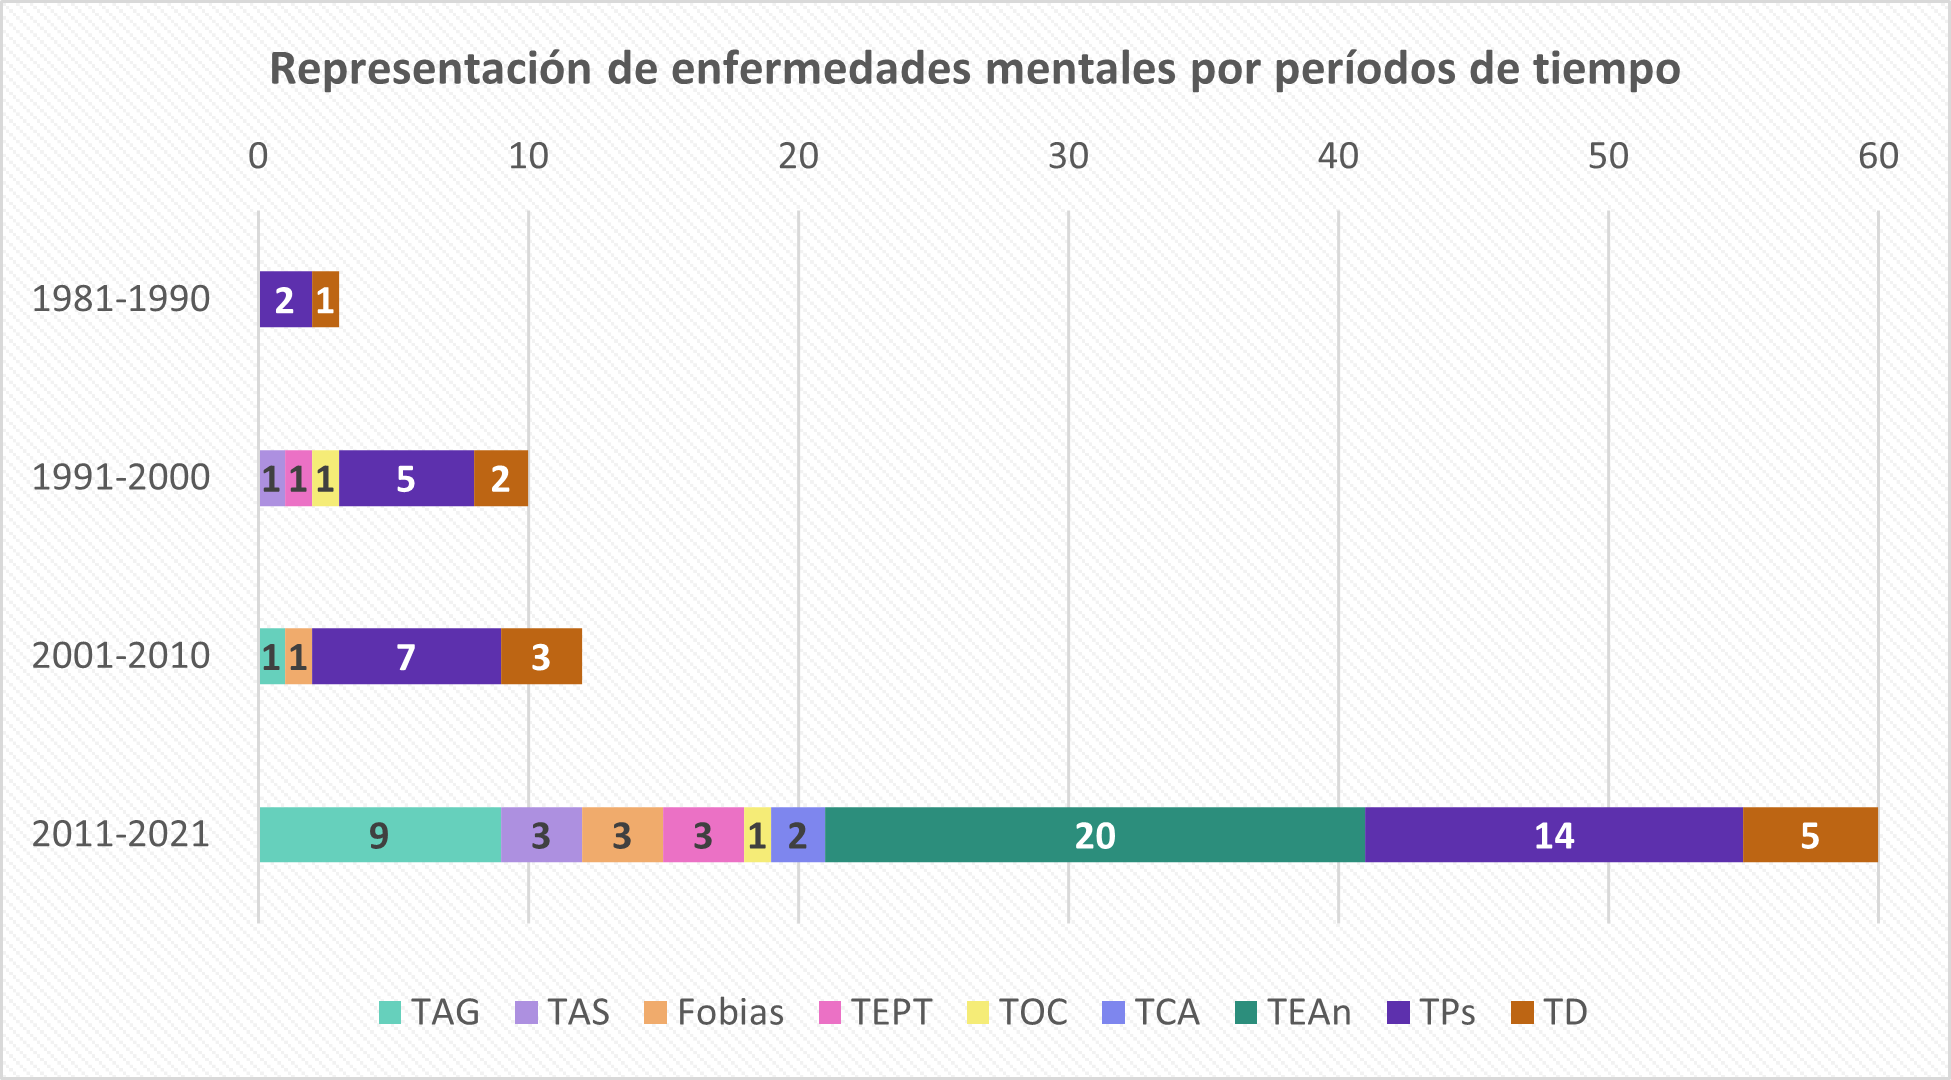
\includegraphics[width=1\linewidth]{Graficas estudio/G1; Enfperiodos.png}
    \caption{Trastornos mentales representados en videojuegos por periodos de tiempo}
    \label{fig:ESTEnfvidtiempo}
\end{figure}

Como puede observarse en la gráfica \ref{fig:ESTEnfvidtiempo}, aparte de que el número de videojuegos ha aumentado en general, se puede ir viendo también la aparición de diferentes enfermedades mentales. Se puede ver claramente que los trastornos psicóticos siguen tomando un papel importante, pero los trastornos del estado de ánimo, generalmente la depresión, han ganado terreno. Estas enfermedades han pasado de no tener representación del 1981 al 2010, a aparecer 20 enfermedades de las 60 enfermedades representadas en los videojuegos seleccionados en el periodo de 2011 a 2021. Se ve también la diferencia claramente en el trastorno de ansiedad generalizada, de haber sólo uno en el periodo de 1981 al 2010, en la etapa más reciente existen 9 videojuegos en los que se representa.


Es también relevante cómo de diferente es la forma de representarse y la importancia de estas enfermedades en el videojuego. Mientras que antes generalmente las enfermedades podían simplemente aparecer y representarse, en mayor o menor medida, teniendo más o menos relevancia, actualmente muchos videojuegos están basados en la propia enfermedad. Sobre todo de las nuevas enfermedades que se han empezado a representar como son la ansiedad o la depresión. Algunos ejemplos de esto son \citetitle{lifeisstrange18} o \citetitle{seasolitude19}.  


\begin{figure}
    \centering
    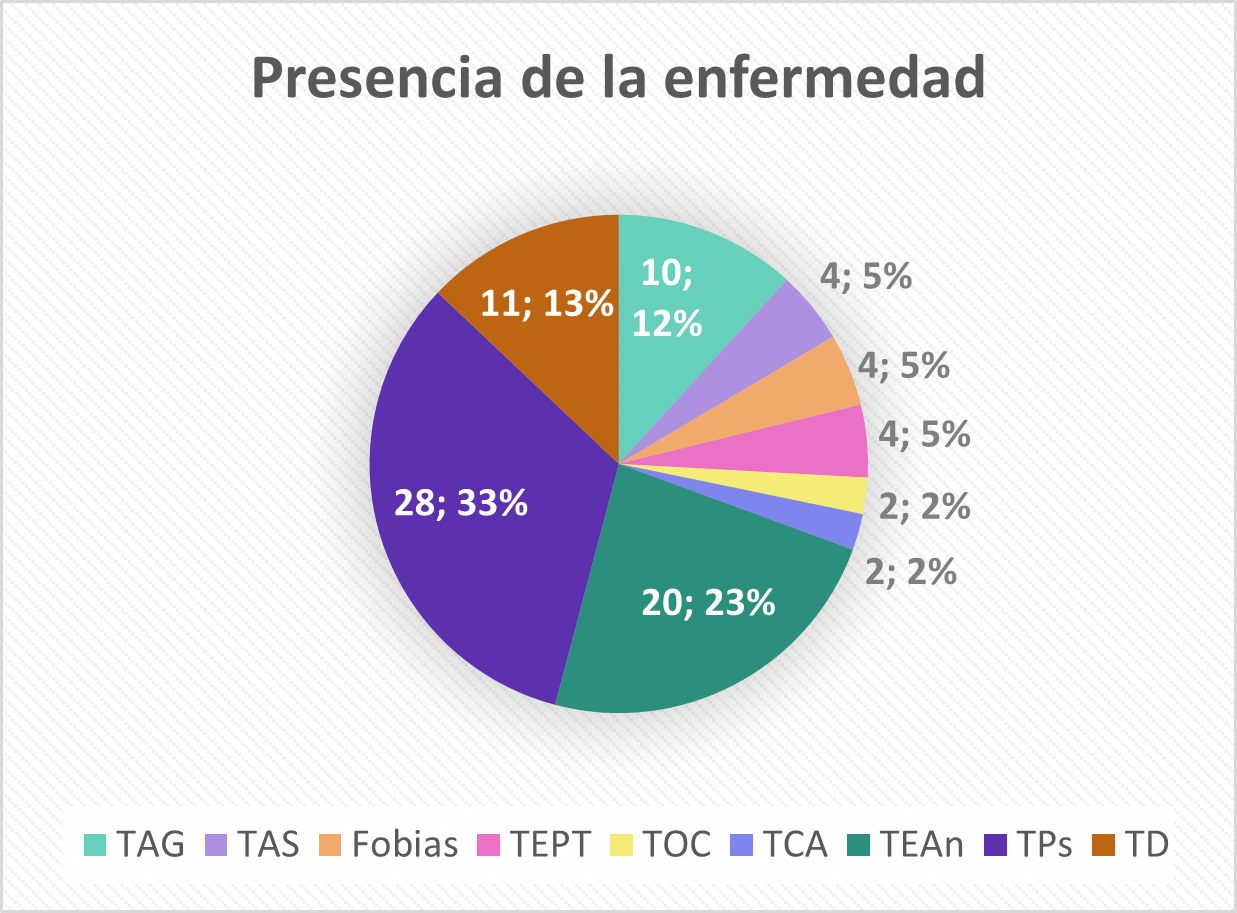
\includegraphics[width=.8\linewidth]{Graficas estudio/G2; PresenciaEnf.png}
    \caption{Enfermedades representadas en videojuegos}
    \label{fig:ESTEnfvid}
\end{figure}


\begin{figure}
    \centering
    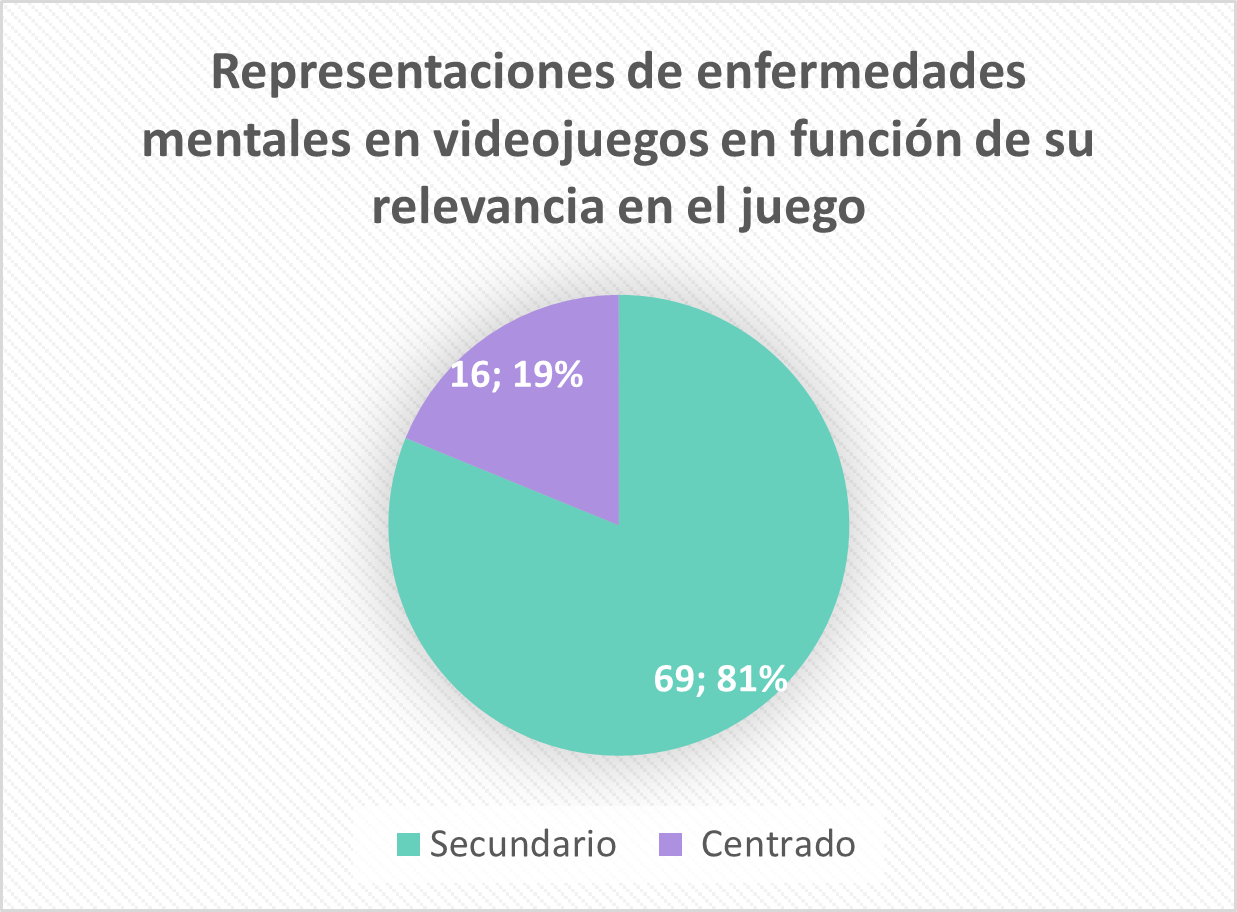
\includegraphics[width=.8\linewidth]{Graficas estudio/G3; RepresentSecun.png}
    \caption{Representación de enfermedades mentales en videojuegos en función de su relevancia en el juego}
    \label{fig:ESTRelevancia}
\end{figure}


Como puede verse en la figura \ref{fig:ESTEnfvid}, agrupando todas las enfermedades mostradas en los videojuegos seleccionados, se puede ver que las enfermedades o trastornos más representados son los trastornos psicóticos, seguidos de los trastornos del estado del ánimo. Sin embargo, esto es gracias a la aparición en los últimos años de videojuegos que muestran otro tipo de enfermedades, puesto que mirando la gráfica \ref{fig:ESTEnfvidtiempo} puede verse que, mientras que los trastornos psicóticos han estado presentes en todos los periodos de tiempo, los trastornos del estado del ánimo sólo aparecen en los videojuegos del último periodo analizado, entre 2011 y 2021. 



Sin embargo, esta representación no siempre da la misma importancia a la enfermedad, hay videojuegos en los que el tema central es el trastorno mental o este tiene una gran importancia dentro de él, mientras que otros lo muestran como un hecho secundario. Entre los videojuegos seleccionados, un total de 56, entre los que se encuentra la demo desarrollada en este mismo trabajo, se pueden encontrar un total de 85 enfermedades representadas. Como puede verse en la figura \ref{fig:ESTRelevancia} sólo el 19\% de estas representaciones son de enfermedades tratadas como elemento central en el videojuego, siendo el 81\% restante representaciones más vagas, con menor relevancia en el videojuego, etc. Esto no necesariamente implica que sea una peor representación, simplemente que no es un elemento relevante en la historia, por el motivo que sea. 



\begin{figure}
\centering
\begin{subfigure}{.5\textwidth}
  \centering
  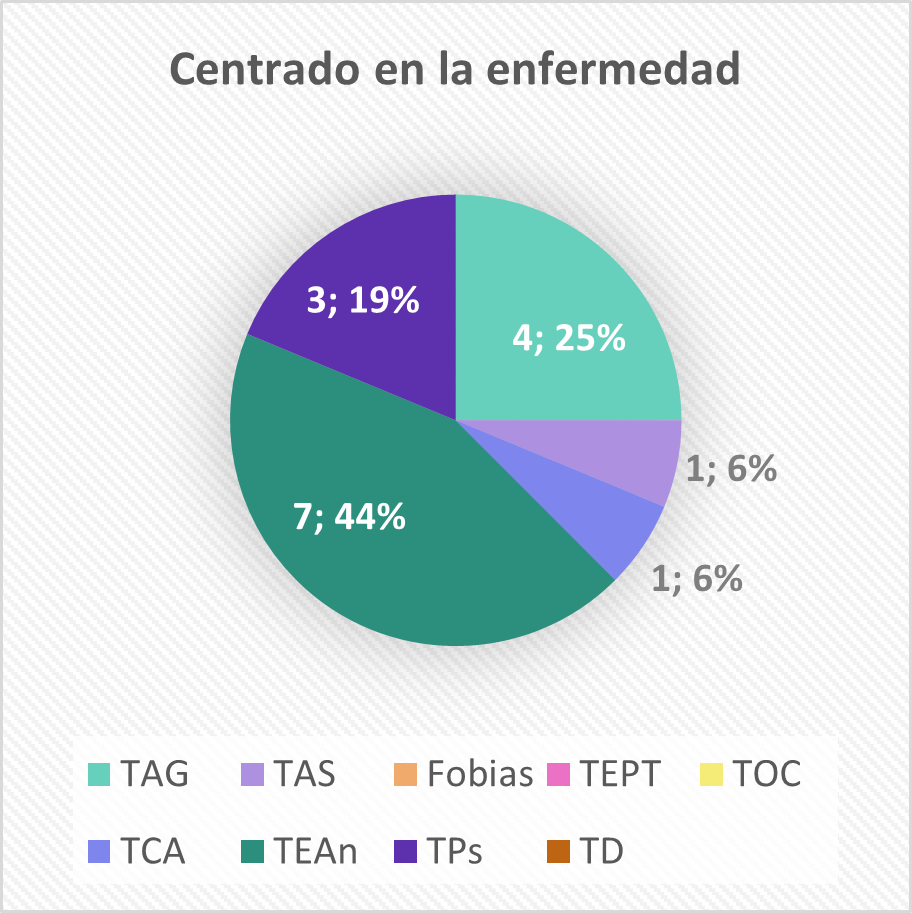
\includegraphics[width=.95\linewidth]{Graficas estudio/G4; Enfcentrado.png}
  \caption{Enfermedades representadas en videojuegos centrados en la enfermedad}
\end{subfigure}%
\begin{subfigure}{.5\textwidth}
  \centering
  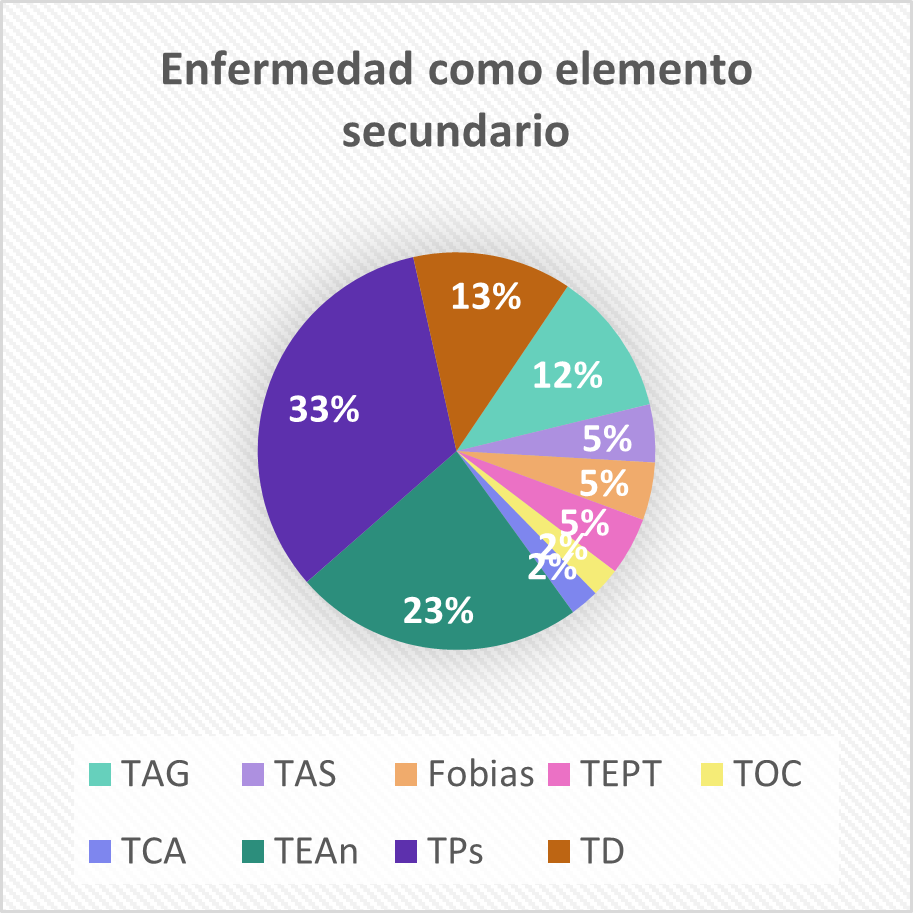
\includegraphics[width=.95\linewidth]{Graficas estudio/G5; Enfsecund.png}
  \caption{Enfermedades representadas en videojuegos como un elemento secundario}
\end{subfigure}
\caption{Representación de trastornos mentales en videojuegos}
\label{fig:ESTEnfcensec}
\end{figure}


Haciendo ahora una distinción entre aquellas representaciones que están centradas en la enfermedad y las que son un hecho secundario, se puede diferenciar también el tipo de trastornos mostrados. Como se puede ver en la figura \ref{fig:ESTEnfcensec}, las enfermedades que se muestran como elemento central en el videojuego son generalmente trastornos del estado del ánimo, seguidos del trastorno de ansiedad generalizada y de los trastornos psicóticos. Por otro lado, entre las representaciones que muestran la enfermedad como un elemento secundario se puede encontrar sobre todo la representación de trastornos psicóticos, seguido de trastornos del estado del ánimo y trastornos disociativos. 



\begin{figure}
    \centering
    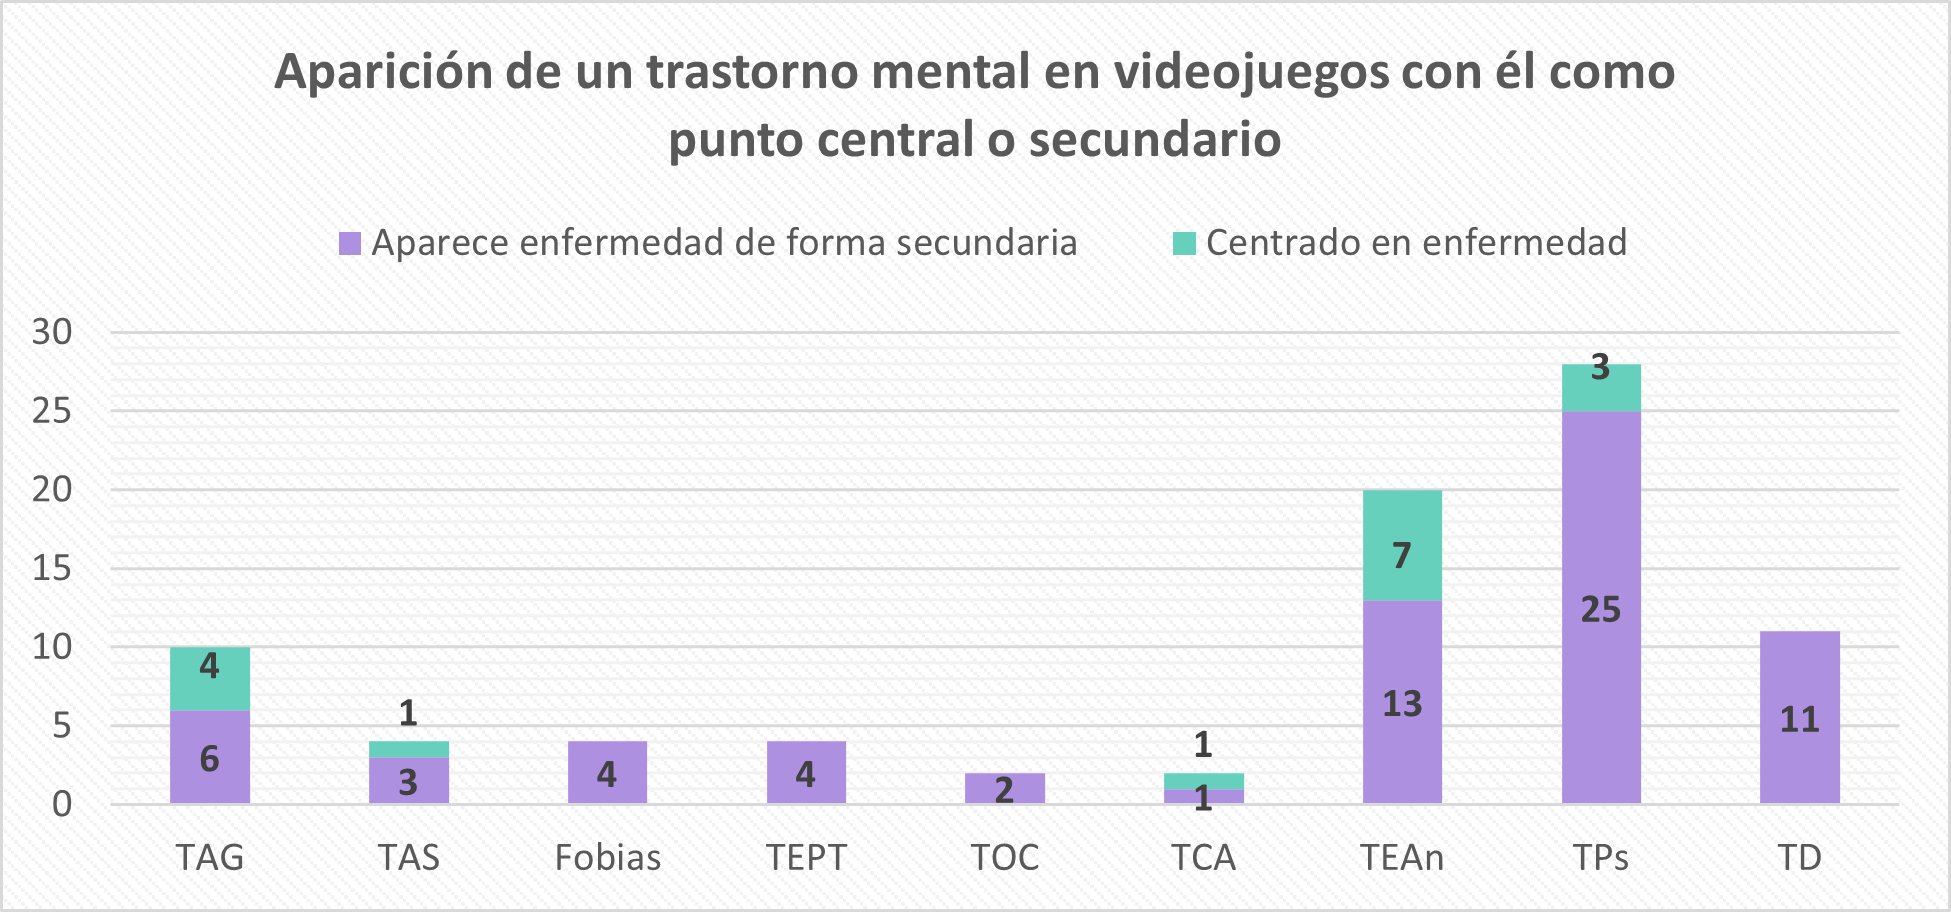
\includegraphics[width=1\linewidth]{Graficas estudio/G6; Enfcentralsecund.png}
    \caption{Representación de enfermedades mentales en videojuegos como punto central o secundario}
    \label{fig:ESTEnfvidcensec}
\end{figure}


    
Por último, en la figura \ref{fig:ESTEnfvidcensec}, se puede observar la frecuencia de aparición de cada tipo de trastorno y la importancia que tiene la enfermedad dentro del videojuego. Se puede observar más claramente cómo hay enfermedades que sólo se tratan de forma secundaria, entre las que se encuentran las fobias, el TEPT, los trastornos disociativos o el TOC, que se pueden encontrar en videojuegos como \citetitle{darkest15} o  \citetitle{tombraider15}. Otros trastornos como los TEAn suelen ser un elemento central en la historia del videojuego más frecuentemente, se puede encontrar en videojuegos como \citetitle{gris18}, \citetitle{thecat12} o \citetitle{actual13}. 








\subsection{En función de las otros aspectos} 
    



Analizando por otro lado otras propiedades o características de estos mismos videojuegos, entre las que se encuentran si han sido desarrolladas y o distribuidas por empresas indies o son considerados AAA (al ser producidos o distribuidos por una distribuidora importante y con un gran presupuesto). Otro elemento analizado ha sido la forma de representación de las enfermedades, en tanto que pueden ser de forma literal o metafórica. Algunos videojuegos representan un trastorno y la evolución de éste como el avance en el videojuego, como ocurre en el juego \citetitle{celeste18} donde se escala una montaña. Otros, sin embargo, tratan la enfermedad de forma literal como ocurre en \citetitle{depression13}, donde se permite al jugador elegir entre varias opciones la siguiente acción de un personaje que padece depresión. A medida que la enfermedad avanza algunas opciones van siendo tachadas, y las opciones que tiene el jugador a veces se reducen a dormir en la cama o en el sofá. 

A continuación, se ha procedido a categorizar al representante de la enfermedad, si es un personaje o elemento protagonista, antagonista (en el caso de ser un enemigo al que derrotar, por ejemplo), o si se trata de forma secundaria. 

Otra columna indica si el juego muestra alguno de los síntomas de la enfermedad que está mostrando o no y por último si se preserva el estigma que existe sobre las enfermedades mentales, basándose la representación en estereotipos, atribuyendo la enfermedad a enemigos a los que derrotar pues la enfermedad los hace violentos, o considerando que los enfermos mentales son personas a las que evitar. 

Como puede verse, esta es una categorización que, dentro de haber intentado ser lo más imparcial posible, posee cierta subjetividad. 





    


\begin{landscape}
\begin{footnotesize}
    \begin{longtable}{l  l  *{15}{c} }
    
      \caption[Análisis de la presencia de trastornos mentales en los Videojuegos]{Análisis de la presencia de trastornos mentales en los Videojuegos\\`s' sí ; `-' no.}
      \label{tab:tablaTipologia}
      \endfirsthead
    \caption[]{Continuación}\\
      \toprule
      &                              & AAA  & Indie  & Literal & Metafórica   &   Protagonista & Antagonista                   & Secundario                  &      Síntomas             &     Estigma              &\\  
      \midrule
      \endhead  % header material
      \midrule
      \multicolumn{11}{r}{\relsize{-.5} Continúa en la página siguiente}\\
      \endfoot  % footer material
      \endlastfoot  % footer material
\toprule
                  
                  
                  & \multirow{2}{*}{}            & \multicolumn{2}{c}{Desarrollo} & \multicolumn{2}{c}{Representación} & \multicolumn{3}{c}{Personaje}  & \multirow{2}{*}{Síntomas} & \multirow{2}{*}{Estigma} \\ \cline{3-4}\cline{5-7}\cline{8-9}
                      &                              & AAA  & Indie  & Literal & Metafórica   &   Protagonista & Antagonista                  & Secundario                  &                   &                   &                   \\
\midrule
\multirow{4}{*}{\rotatebox{90}{1981-1990}} & \citetitle{jekyll88}	     &   -   & s     & s   & -   & s  & - & -   & s    & s     \\
                      & \citetitle{psycosis90}		     &   -   & s     & -   & s   & s  & -   &- & -    & -     \\
                      \midrule     
\multirow{6}{*}{\rotatebox{90}{1991-2000}} & \citetitle{smartpatrol96}   &    -   & s     & s   & -   & s  &- & -   & -    & s     \\
                      & \citetitle{ff797}	     &   s   & -     & s   & -   & s &- & s   & s    & -     \\
                      & \citetitle{jugger98}		     &    -   & s     & -   & s   & -  & - & s   & -    & s     \\
                      & \citetitle{sanit98}		     &  -   & s     & s   & -   & s & -  & s   & s    & s     \\
                      & \citetitle{planet99}		     &   -   & s     & s   & -   & s & -  & -   & s    & -     \\

                      & \citetitle{alice00}	   & s   & s     & s   & -   & s  &- & -   & s    & s     \\
\midrule
\multirow{12}{*}{\rotatebox{90}{2001-2010}} & \citetitle{jekyll01}		     &    -   & s     & s   & -   & s  & - & -   & s    & s     \\
                      & \citetitle{silent01}		     &  s   & -     & s   & s   & s  &- & s   & -    & s     \\
                      & \citetitle{eternal02}	     &    s   & s     & s   & -   & s  & s & -   & s    & s     \\
                      & \citetitle{suffer04}		     &   -   & s     & s   & -   & s &- & -   & -    & s     \\
                      & \citetitle{killer05}			     &   -   & s     & s   & -   & s  & - & -   & s    & -     \\
                      & \citetitle{crush07}			     &  s   & s     & -   & s   & s  & - & -   & -    & -     \\
                      & \citetitle{manhunt07}		     &   s   & -     & s   & -   & s  & - & -   & s    & s     \\
                      & \citetitle{haze08}			     &   s   & s     & s   & -   & s  &- & -   & s    & s     \\
                      & \citetitle{batman09}	     &   s   & -     & s   & -   & -  & -  & s   & -    & s     \\
                      & \citetitle{dreamkiller09}		     &   -   & s     & s   & s   & s  & - & s   & -    & s     \\
                      & \citetitle{deadspace08}		     &   s   & -     & s   & -   & s  & -  & -   & s    & s   \\ 
\newpage
\multirow{23}{*}{\rotatebox{90}{2011-2021}} & \citetitle{alice11}	     &    s   & s     & s   & -   & s  & -  & -   & s    & s     \\
                      & \citetitle{lanoire11}	      	     &   s   & s     & s   & -   & -  & - & s   & -    & s     \\
                      & \citetitle{thecat12}      	     &     -   & s     & s   & -   & s  & -  & -   & s    & -     \\
                      & \citetitle{farcry12}      	     &s   & -     & s   & -   & - & s  & -   & -    & s     \\
                      & \citetitle{actual13}	             &     -   & s     & s   & -   & s  & - & -   & s    & -     \\
                      &\citetitle{depression13}	     &    -   & s     & s   & -   & s  & - & -   & s    & -     \\
                      & \citetitle{outlast13}			     &    -   & s     & s   & -   & -  & - & s   & -    & s     \\
                      & \citetitle{blackbay14}		     &  -   & s     & s   & -   & s & -  & -   & -    & s     \\
                      & \citetitle{etherone14}		     &    -   & s     & -   & s   & s  &  - & -   & s    & -     \\
                      & \citetitle{evilwithin14}	     &   s   & -     & s   & -   & s & -  & s   & s    & s     \\
                      & \citetitle{neverending14}	     &  -   & s     & s   & -   & s & -  & -   & s    & -     \\
                      & \citetitle{batman15}    &   s   & -     & s   & -   & -  & - & s   & -    & s     \\
                      & \citetitle{darkest15}		     &  -   & s     & s   & -   & s  & - & -   & -    & -     \\
                      & \citetitle{franbow15}		     &   -   & s     & s   & s   & s  & - & -   & s    & -     \\
                      & \citetitle{pry15}		     &  -   & s     & s   & -   & s  & - & -   & s    & -     \\
                      & \citetitle{tombraider15}    &   s   & -     & s   & -   & s  & -  & -   & -    & -     \\
                      & \citetitle{sym15}			     &  -   & s     & -   & s   & s & -  & -   & -    & -     \\
                      & \citetitle{untildawn15}		     &    s   & s     & s   & -& - & s  & -   & -    & s     \\
                      & \citetitle{beginners15}             &   -   & s     & -   & s   & s & -   & -   & -    & -      \\
                         &\citetitle{desire16}       &   -   & s     & -   & s   & s  & - & s   & s    & -     \\
                      & \citetitle{layers16}              & -   & s     & s   & -   & s & - & -   & s    & -     \\
                      & \citetitle{tharsis16}                     &   -   & s     & s   & -   & s & - & -   & s    & s     \\
                      & \citetitle{dragon16}          &   -   & s     & -   & s   & s & - & -   & -    & -     \\                                               
\multirow{14}{*}{\rotatebox{90}{2011-2021}} & \citetitle{town16}            &    -   & s     & s   & -   & s  & -& -   & s    & s     \\
                      & \citetitle{doki17}  &    -   & s     & s   & -   & s& -  & -   & s    & -     \\
                      & \citetitle{fractured17}              &    -   & s     & -   & s   & s & - & -   & s    & -     \\
                      & \citetitle{hellblade17} &  s   & -     & s   & -   & s & - & -   & s    & -     \\
                      & \citetitle{lastday17}             &   -   & -     & s   & -   & s & - & s   & -    & s     \\
                      & \citetitle{night17}           &  -   & s     & s   & -   & s & - & s   & s    & -     \\
                      & \citetitle{celeste18}                      &   -   & s     & -   & s   & s & - & -   & -    & -     \\
                      & \citetitle{gris18}                        &   -   & s     & -   & s   & s & - & -   & -    & -     \\
                      & \citetitle{heartbound18}                   &  -   & s     & s   & -   & s & - & -   & s    & -     \\
                      & \citetitle{lifeisstrange18}             &   s   & s     & s   & -   & s  & s & s   & s    & -     \\
                      & \citetitle{redsting18}        &  -   & s     & -   & s   & - & - & s   & -    & -     \\
                      & \citetitle{seasolitude19}              &   s   & s     & -   & s   & s& -  & -   & -    & -     \\
                      & \citetitle{tellmewhy20}                  &  s   & -     & s   & -   & s & - & -   & s    & -     \\
                      & \citetitle{elmio}                       &   -   & s  & s      & -   & s   & -  & - & -   & s   & -    \\
\bottomrule
                    \end{longtable}
                    \end{footnotesize}
\end{landscape}








\begin{figure}
\centering
\begin{subfigure}{.5\textwidth}
  \centering
  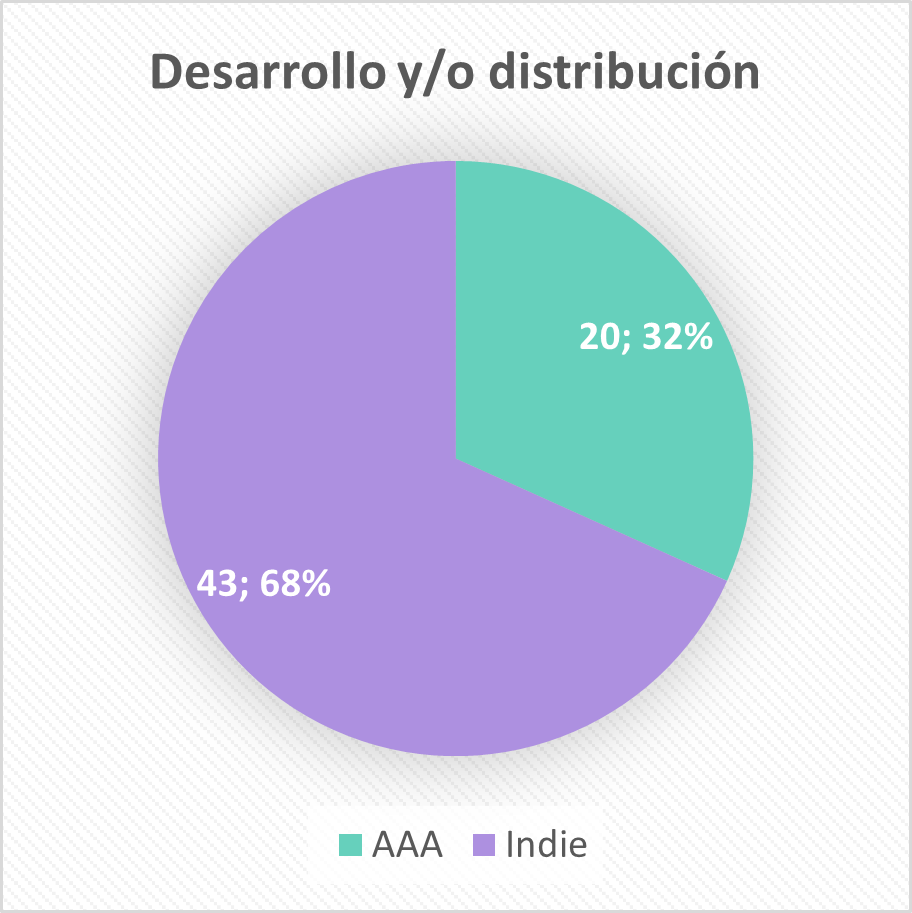
\includegraphics[width=.95\linewidth]{Graficas estudio/G7;Desarrollo.png}
  \caption{Desarrollo y distribución}
\end{subfigure}%
\begin{subfigure}{.5\textwidth}
  \centering
  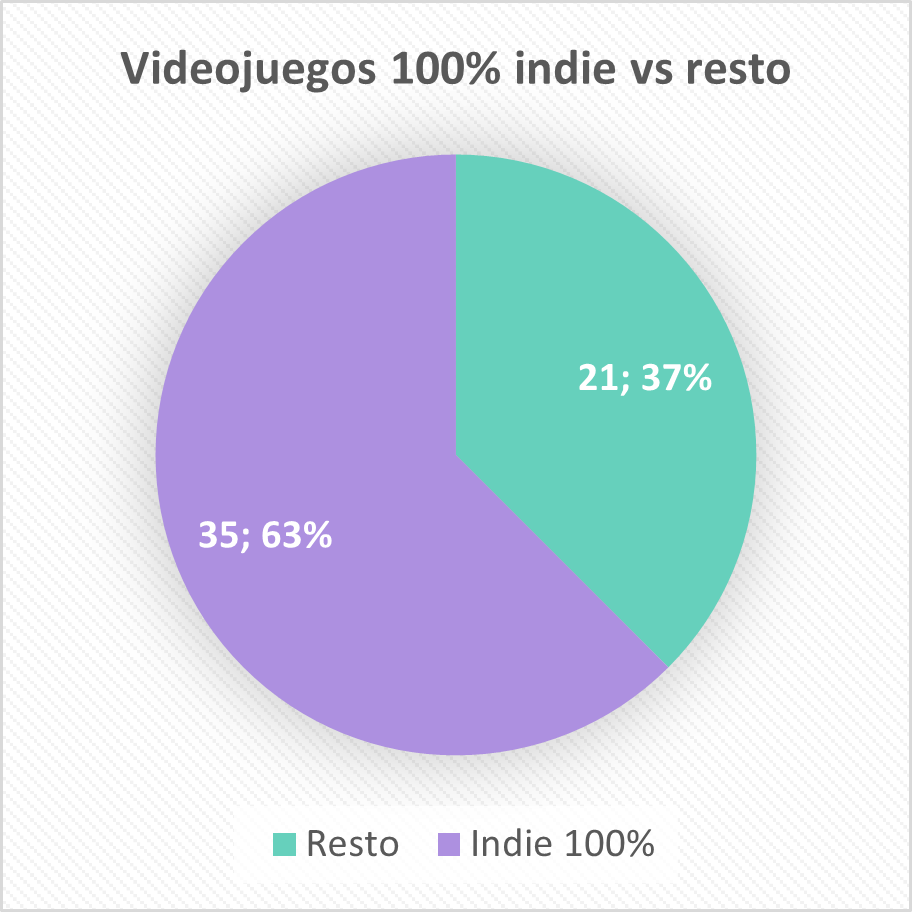
\includegraphics[width=.95\linewidth]{Graficas estudio/G8;DesarrolloIndie.png}
  \caption{Comparativa de videojuegos 100\% indie vs. los demás}
  \label{fig:ESTjuegosindie}
\end{subfigure}
\caption{Desarrollo y distribución de videojuegos que representan enfermedades mentales}
\label{fig:ESTDesarrollo}
\end{figure}



Los resultados de este estudio se pueden encontrar en la tabla \ref{tab:tablaTipologia}. En el caso del desarrollo y/o distribución, de los videojuegos seleccionados, sólo un 32\% son considerados AAA o bien han sido distribuidos o publicados por una empresa de gran importancia. El 68\% han sido realizados o distribuidos por empresas indie generalmente con bajo presupuesto. (Véase la figura \ref{fig:ESTDesarrollo}). Hay algunos videojuegos, como \citetitle{untildawn15} que pertenece a ambas categorías al estar desarrollado por una empresa indie, \cite{supermassive}, pero distribuido por \cite{sony}. Los videojuegos desarrollados y distribuidos al 100\% por empresas indie desciende a un 63\%, como puede verse en la figura \ref{fig:ESTjuegosindie}. 




\begin{figure}
\centering
\begin{subfigure}{.4\textwidth}
  \centering
  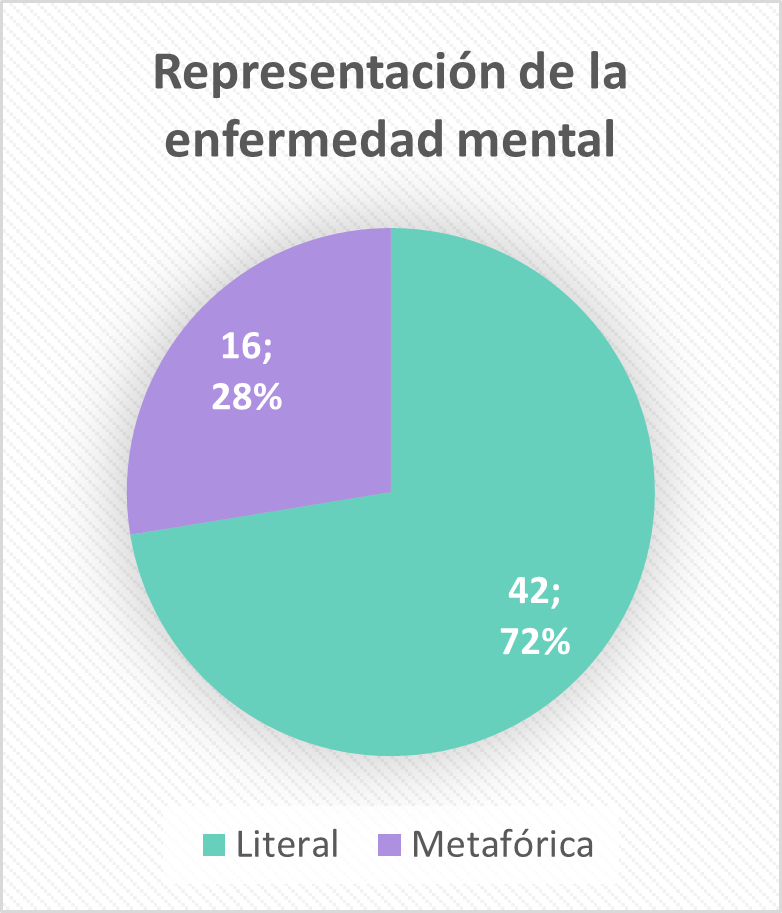
\includegraphics[width=.95\linewidth]{Graficas estudio/G9; Repmetlit.png}
  \caption{Representación de la enfermedad mental}
\end{subfigure}%
\begin{subfigure}{.6\textwidth}
  \centering
  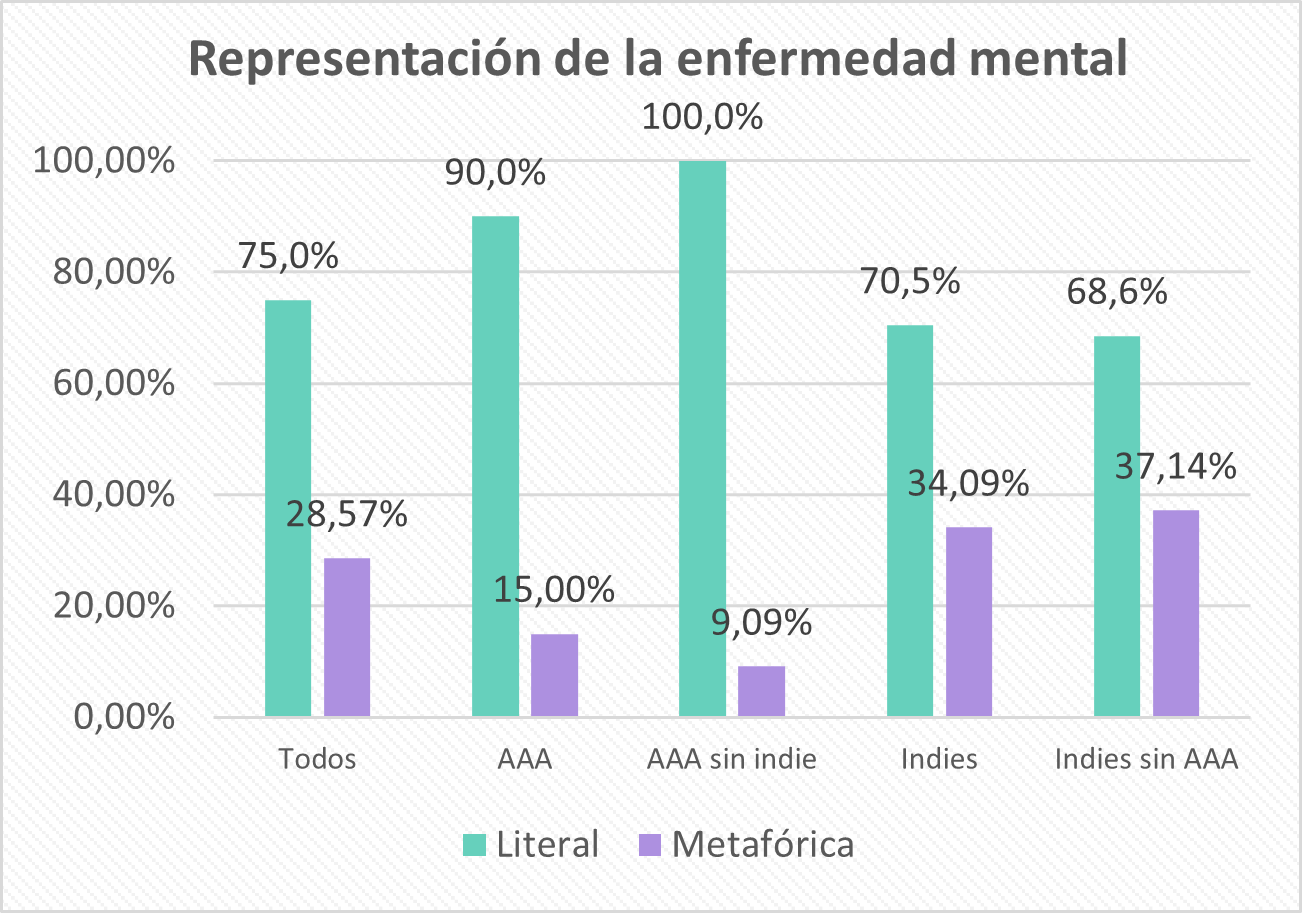
\includegraphics[width=.95\linewidth]{Graficas estudio/G10; RepmetlitVS.png}
  \caption{Representación de la enfermedad en función del desarrollador/distribuidor}
\end{subfigure}
\caption{Comparación de la representación de las enfermedades mentales de forma literal o metafórica}
\label{fig:ESTrepresentacion}
\end{figure}



La representación de las enfermedades mentales es, en un 72\%, literal, como puede verse en la figura \ref{fig:ESTrepresentacion}. Haciendo una distinción entre los tipos de videojuego en función de su desarrollo y distribución, se obtienen que la mayor proporción de videojuegos donde se puede encontrar una representación metafórica, siendo de un 37\% de los datos, se encuentra en los juegos 100\% indie. Hay videojuegos donde se puede encontrar representación tanto literal como metafórica, como es el caso de \citetitle{celeste18}, donde aparte de la representación metafórica de la montaña, el personaje, por ejemplo, sufre un ataque de ansiedad que se representan de forma literal, sin ningún tipo de metáfora, con un ruido intenso que incluso el jugador desea que acabe, pero no puede hacerlo acabar al tratarse de una cinemática. Tras esto se enseña una técnica de relajación, de la que posteriormente se hablará en la sección \ref{sec:videojuegosEnf}.



\begin{figure}
	\centering
	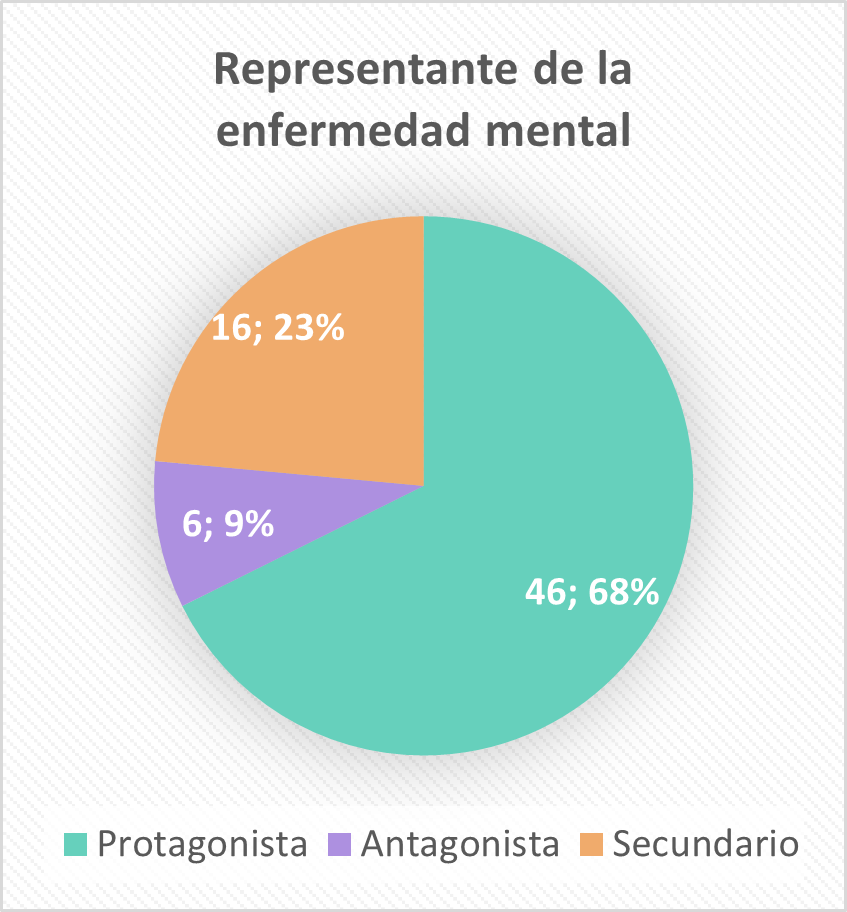
\includegraphics[width=.6\linewidth]{Graficas estudio/G11; Representante.png}
	\caption{Representante de la enfermedad mental en el videojuego}
	\label{fig:ESTRepresentante}
\end{figure}


\begin{figure}
	\centering
	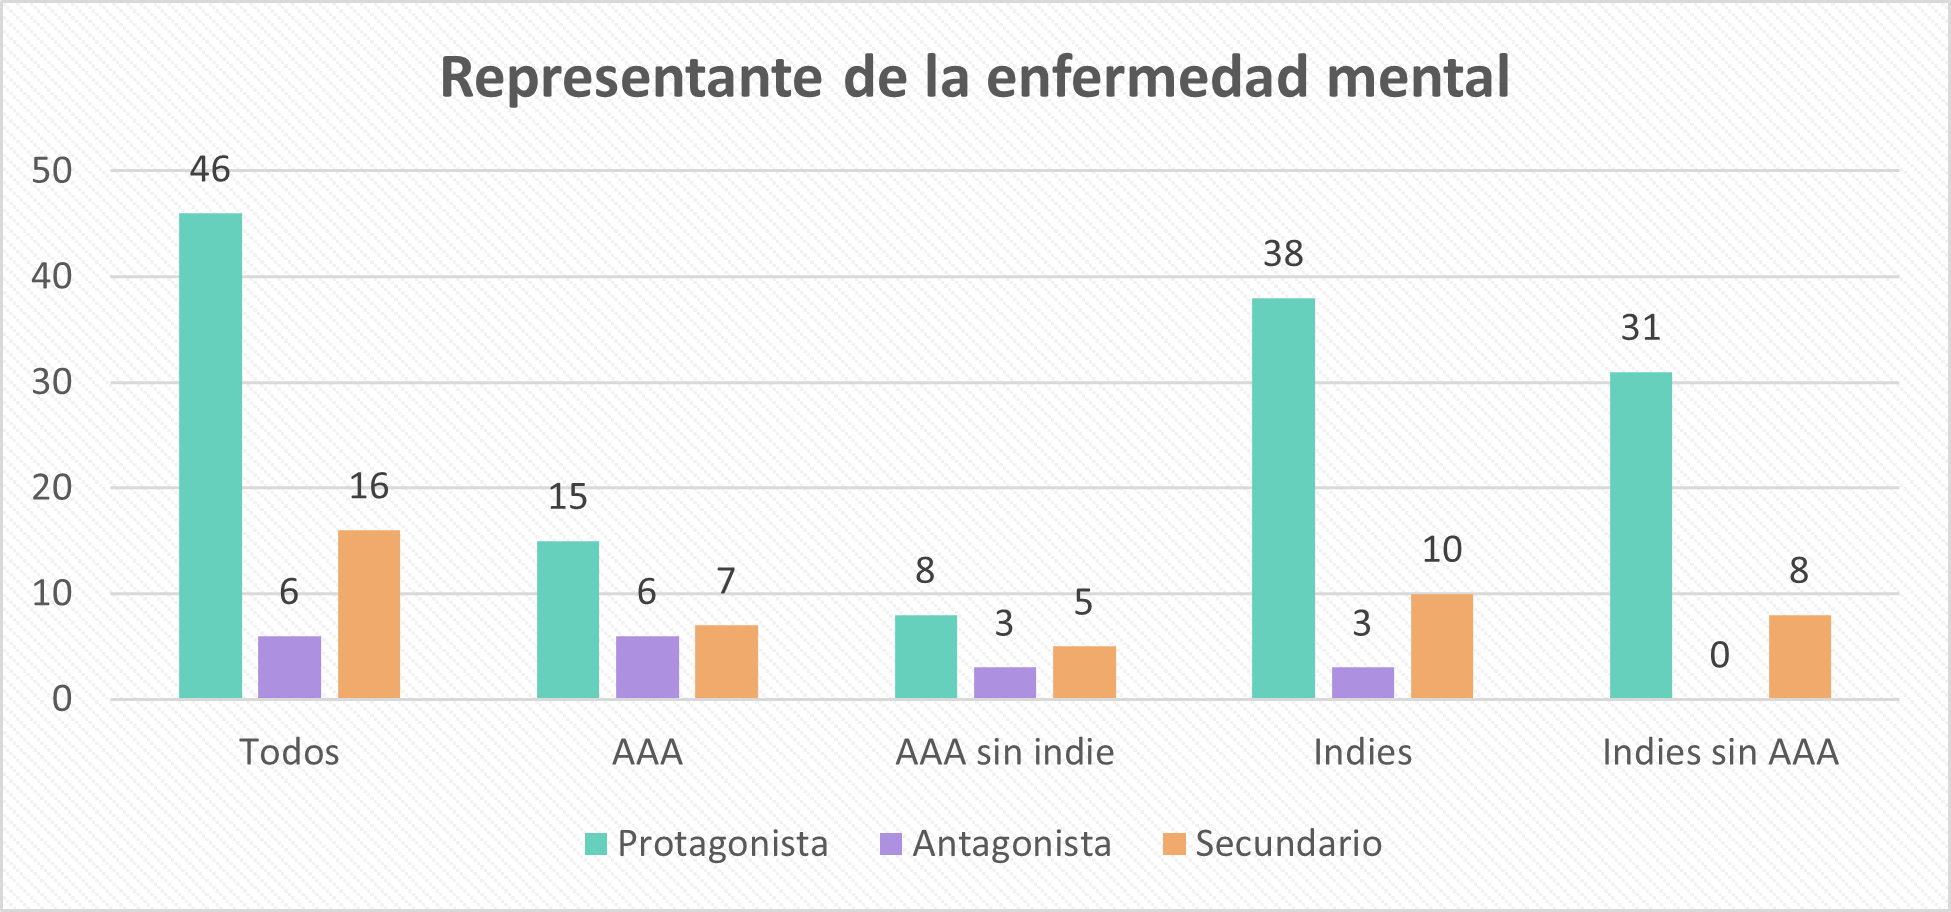
\includegraphics[width=.8\linewidth]{Graficas estudio/G12; RepresentanteVS.png}
	\caption{Representante de la enfermedad mental en el videojuego en función del desarrollador/distribuidor}
	\label{fig:ESTRepresentanteVS}
\end{figure}



En cuanto al representante de la enfermedad, entre protagonista, antagonista y secundario, en la mayoría de los casos, en los videojuegos seleccionados, se trata del protagonista el que tiene la enfermedad y la representa de algún modo. Sólo el 9\% de las veces que se representa se hace en forma de antagonista. (Véase la figura \ref{fig:ESTRepresentante}). No obstante, estos resultados son diferentes si se analizan en función del desarrollador o distribuidor, como puede verse en la figura \ref{fig:ESTRepresentanteVS}. En el caso de los juegos 100\% indies, no hay ningún caso en el que haya una representación en un antagonista, y sólo un 6,8\% en el caso de tener colaboración por parte de alguna distribuidora de AAA. Por otro lado, en los AAA, un 30\% de ellos representan la enfermedad en forma de antagonista. Casos como \citetitle{batman09}, \citetitle{farcry12} o \citetitle{manhunt07} son un claro ejemplo de estas prácticas. 	   
 



\begin{figure}
\centering
\begin{subfigure}{.5\textwidth}
  \centering
  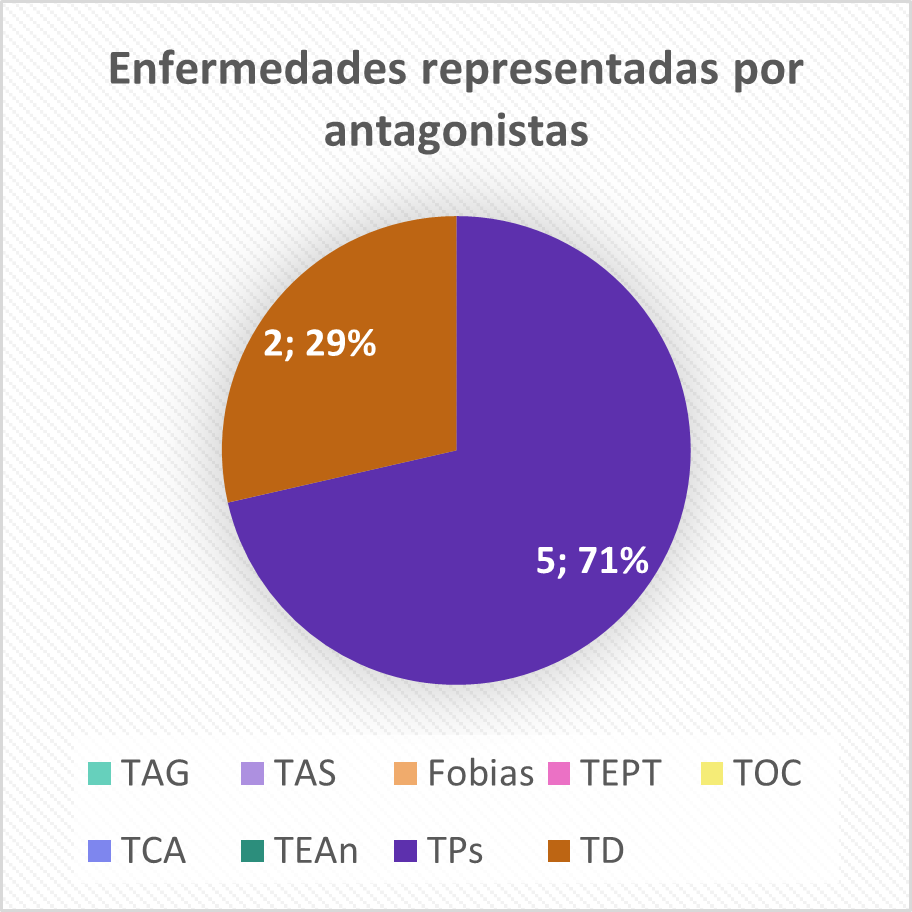
\includegraphics[width=.95\linewidth]{Graficas estudio/G13; Enfanta.png}
  \caption{Enfermedades en videojuegos con antagonistas}
\end{subfigure}%
\begin{subfigure}{.5\textwidth}
  \centering
  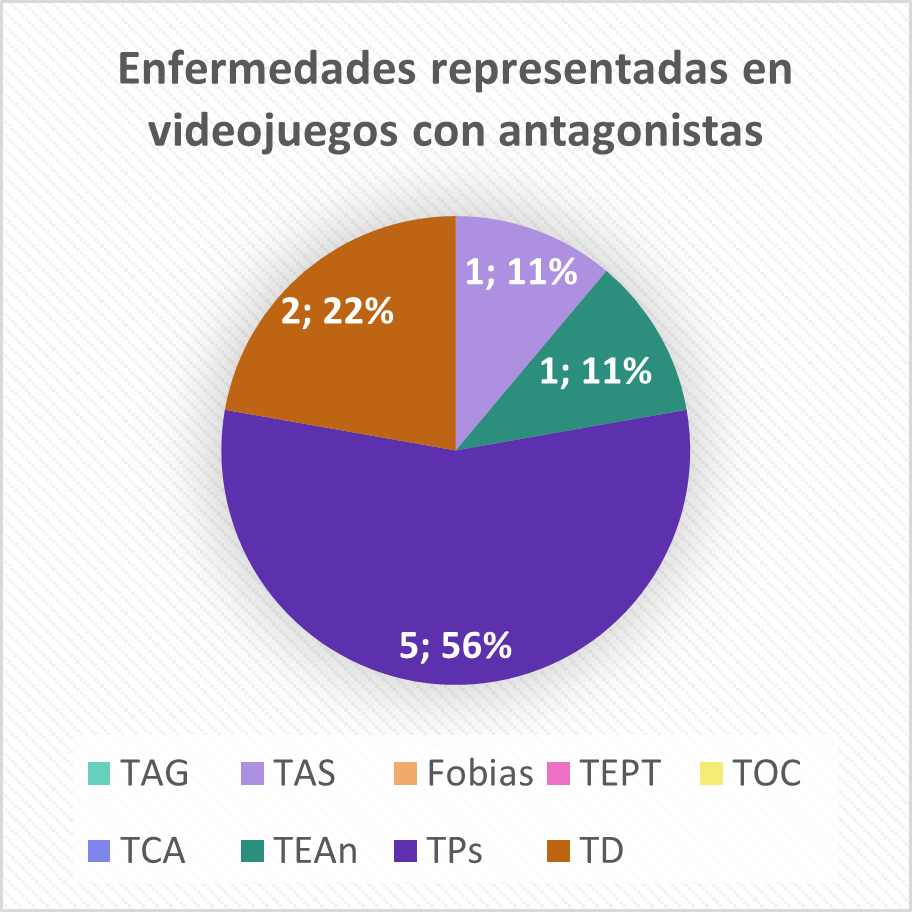
\includegraphics[width=.95\linewidth]{Graficas estudio/G14; Enfvidanta.png}
  \caption{Enfermedades de los antagonistas}
\end{subfigure}
\caption{Enfermedades representadas en videojuegos con antagonistas con enfermedades mentales}
\label{fig:ESTEnfantagonistas}
\end{figure}



 
Relacionando la presencia de antagonistas con las enfermedades representadas por esos videojuegos, se puede ver en la figura \ref{fig:ESTEnfantagonistas} que en su mayoría se trata de TPs. Dado que uno de los videojuegos donde se muestran enfermedades mentales representadas en antagonistas, se representan además otras enfermedades en la protagonista y personajes secundarios, como ocurre en \citetitle{lifeisstrange18}, se ha realizado un nuevo análisis eliminando aquellas enfermedades representadas por el personaje protagonista o secundarios, obteniendo la gráfica de la figura \ref{fig:ESTEnfantagonistas}, donde es aún mayor el porcentaje de representación de TPs, pasando de ser un 56\% a un 71\%. Además, desaparecen dos trastornos, quedándose repartido únicamente entre TPs y TDs, que suelen ser los trastornos más estigmatizados.  


\begin{figure}
    \centering
    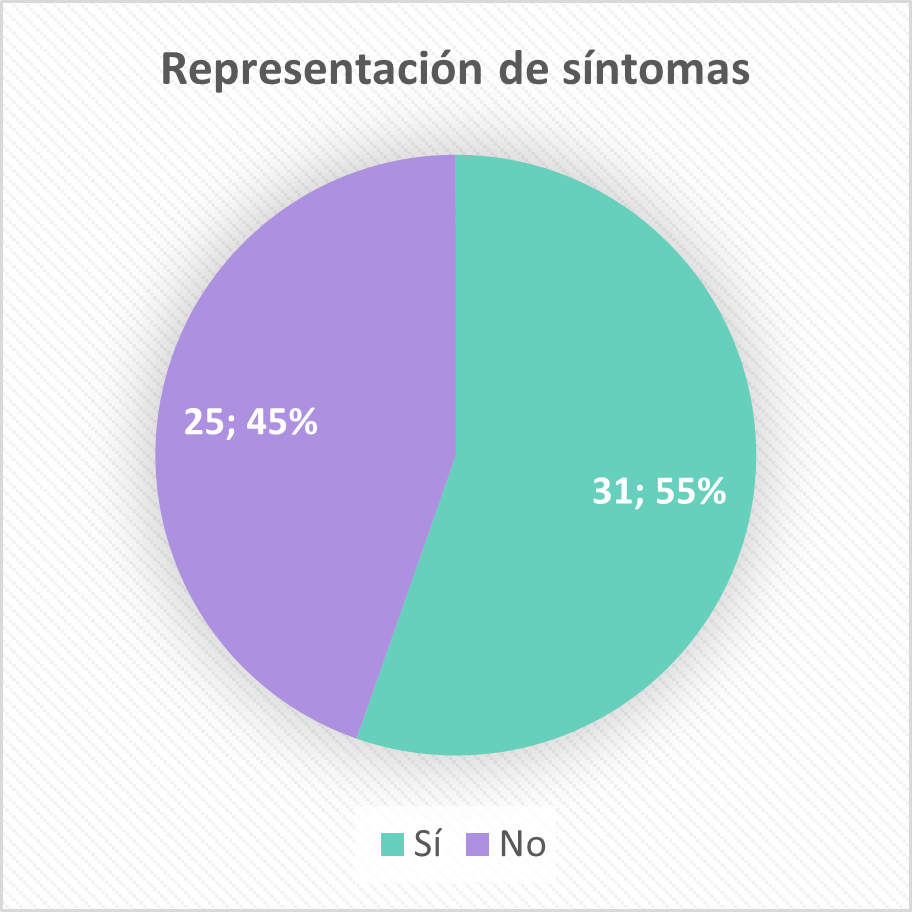
\includegraphics[width=.6\linewidth]{Graficas estudio/G15;Sintomas.png}
    \caption{Representación de síntomas de los trastornos mentales}
    \label{fig:ESTSintomas}
\end{figure}


En cuanto a si representan o no síntomas de la enfermedad que supuestamente se está representando en los videojuegos, se ha considerado que en un 55\% de los casos sí que se hace, en mayor o menor medida. Véase la figura \ref{fig:ESTSintomas}. 

\begin{figure}
\centering
\begin{subfigure}{.4\textwidth}
  \centering
  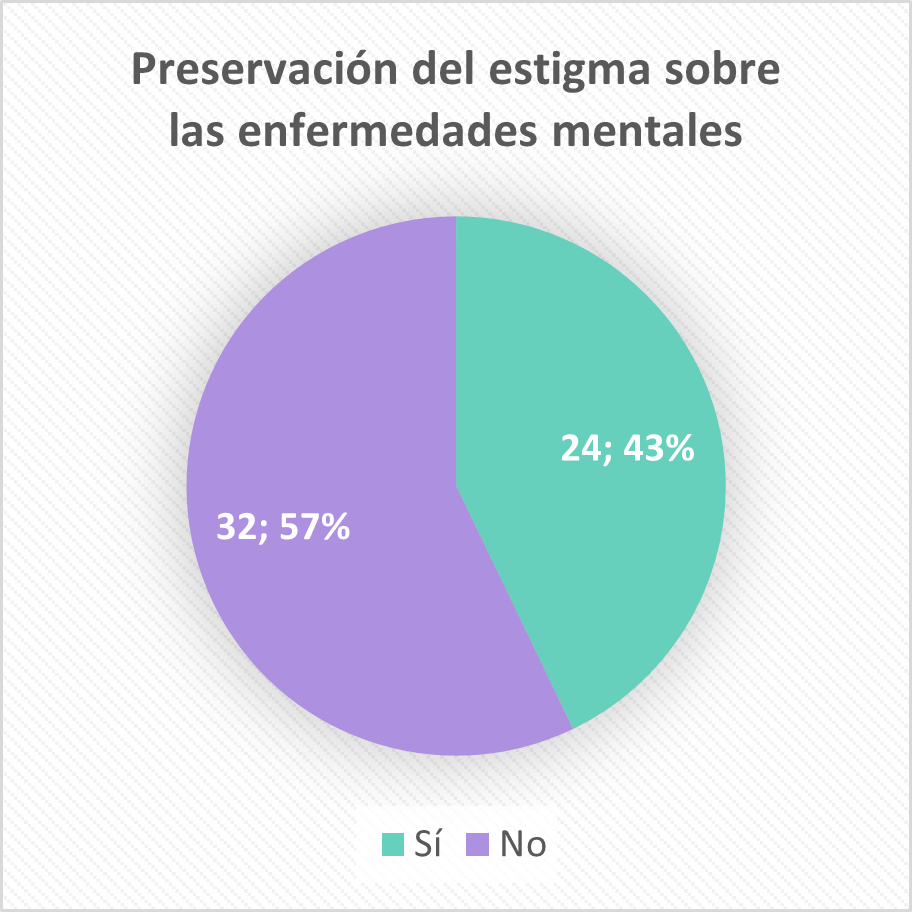
\includegraphics[width=.95\linewidth]{Graficas estudio/G16;Estigma.png}
  \caption{Preservación del estigma}
\end{subfigure}%
\begin{subfigure}{.6\textwidth}
  \centering
  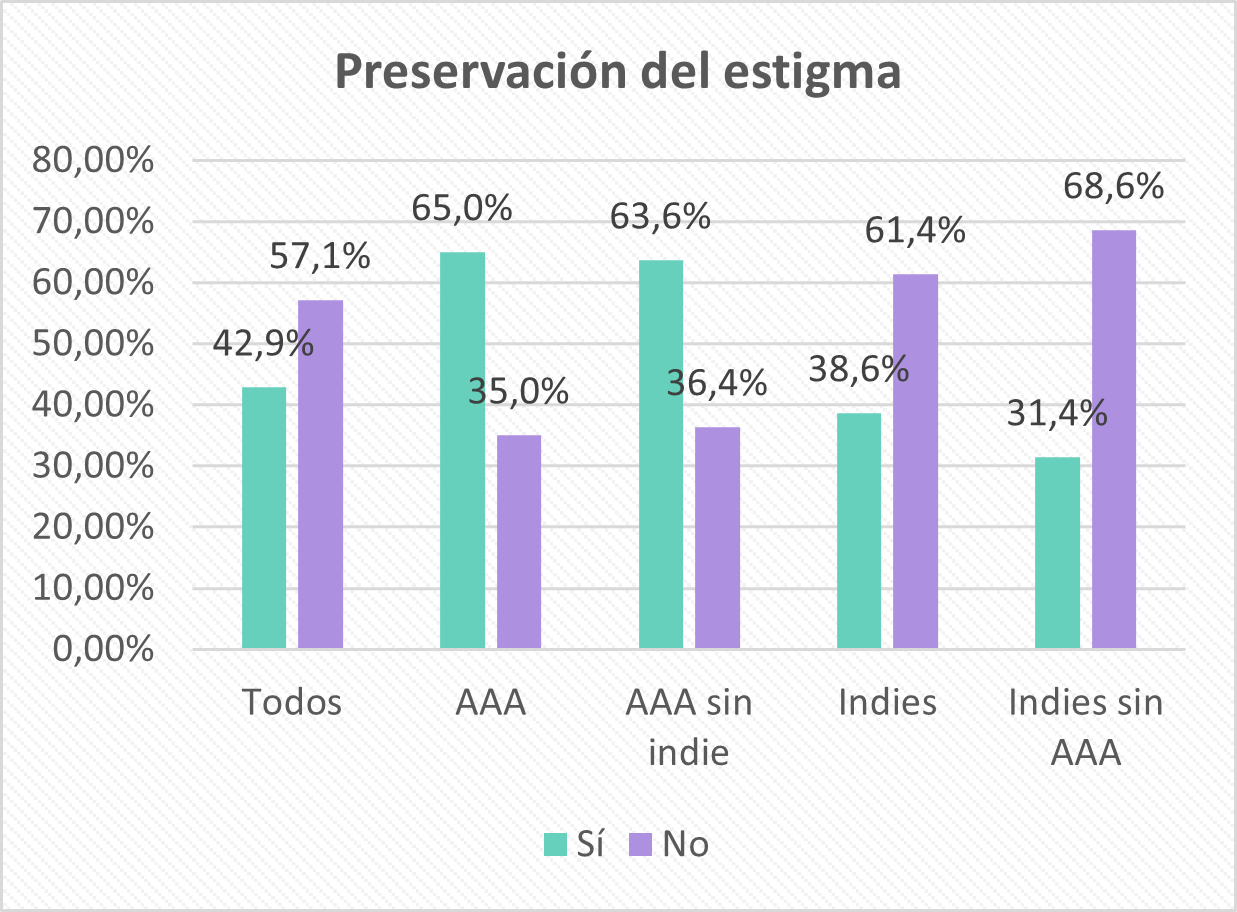
\includegraphics[width=.95\linewidth]{Graficas estudio/G17; EstigmaVS.png}
  \caption{Preservación del estigma en función del desarrollador/distribuidor}
\end{subfigure}
\caption{Preservación del estigma sobre las enfermedades mentales en videojuegos}
\label{fig:ESTEstigma}
\end{figure}


Por último, con respecto a la preservación o no del estigma sobre las enfermedades, se considera que en un 43\% de los casos todavía se estigmatizan. Haciendo una distinción entre los desarrolladores y distribuidores, se puede ver que son los AAA los que suelen preservar más el estigma, siendo un 65\% del total de juegos, aquellos que lo hacen, a diferencia de los juegos 100\% indies, pese a que un 31\% todavía lo hace, como puede verse en la figura \ref{fig:ESTEstigma}

\begin{figure}
    \centering
    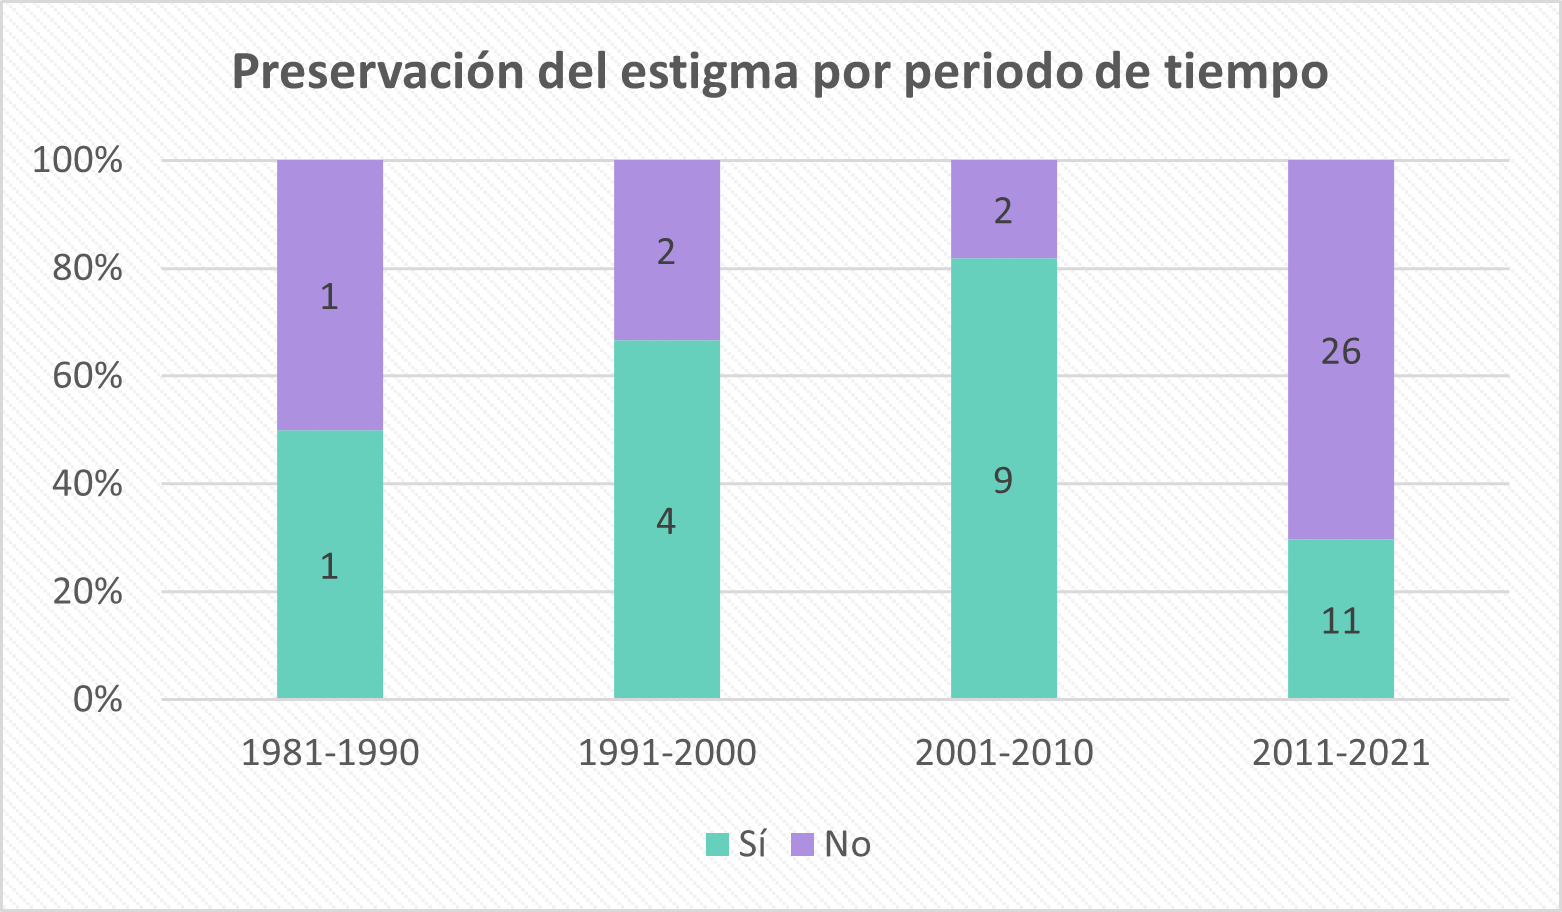
\includegraphics[width=.8\linewidth]{Graficas estudio/G18; EstigmaTiempo.png}
    \caption{Comparación de la preservación del estigma en diferentes periodos de tiempo}
    \label{fig:ESTEstigmatiempo}
\end{figure}

Comparando por periodos de tiempo, y teniendo en cuenta que no en todos los periodos de tiempo se han añadido el mismo número de videojuegos, se puede ver en la gráfica de la figura \ref{fig:ESTEstigmatiempo} que en las décadas anteriores, a medida que iban apareciendo más videojuegos que trataran enfermedades mentales, más de ellos las estigmatizaban. Sin embargo, en esta última década, aparte de un mucho mayor número de videojuegos, el porcentaje de estos en los que se muestra una enfermedad mental desde el punto de vista del estigma ha disminuido considerablemente, pasando de más de un 80\% en la década anterior a un 30\% en la última década. 

El hecho de que cada vez existan más juegos indies y sean más accesibles y más fácilmente conocidos (gracias a la existencia de Steam, Humble Bundle, Epic Games, u otras plataformas de distribución de videojuegos entre otras cosas), favorece la existencia de este tipo de videojuegos diferentes que tratan otras enfermedades mentales y tratan de no estigmatizarlas o al menos, con el paso del tiempo, ir haciéndolo menos. 





\section{Videojuegos que representan enfermedades mentales}
\label{sec:videojuegosEnf}

Centrando la atención en algunos de los videojuegos en particular que representan enfermedades mentales, se analizará de qué manera lo hace cada uno de ellos.

Comenzando por \citetitle{celeste18},  en este videojuego se trata de representar la ansiedad y la depresión a través de sus personajes principales, Madeline y Badeline, su principal enemigo, que nace de ella misma. Madeline tiene como misión subir la Montaña Celeste, proceso en el cual tiene que enfrentar a su yo interior, Badeline, que representa a sus demonios interiores, como son la ansiedad y depresión. Al final consigue entender que no podrá llegar a la cima de la montaña si no es con la ayuda de Badeline, entiende que la ansiedad y la depresión no se van a ir, tiene que intentar aprender a vivir con ellas. 

Este juego, además, tiene un minijuego en el que se ayuda a controlar la respiración, un ejercicio muy útil para aquellas personas que estén sufriendo un ataque de ansiedad o de pánico o que están lidiando con estrés. Algunos usuarios de Reddit agradecen mucho este detalle \textit{``This single feather helped me with so many panic attacks. I freaking love this game.''} \textit{(Esta simple pluma me ayudó con muchos ataques de pánico. Me encanta este juego)}. \cite{featheceleste}. Ver Imagenes \ref{img:featherCelesteA} y \ref{img:featherCelesteB}.  

En este caso, los credaores no consultaron con personal profesional de la salud mental, se basaron en las experiencias de uno de los desarrolladores para construir la historia y reflejar las enfermedades mentales representadas. 
Como se ha mencionado, la representación de la enfermedad se hace sobre todo a través de los personajes y la historia del videojuego. En cuanto a las mecánicas, se trata de un juego de plataformas, donde cabe remarcar como mecánica principal el hecho de morir. Se necesita morir varias veces en algunas ocasiones para conseguir avanzar con el juego, ya que se necesita de una gran precisión. Podría considerarse esto también un guiño a la historia de superación, que no importa cuantas veces caigas, que puedes levantarte y superar el desafío que se está atravesando, bien sea en forma de plataformas, bien en forma de un trastorno mental, donde suele atravesarse en forma de montaña rusa. Como escriben en el artículo \textit{``Celeste y el potencial del videojuego para tratar la ansiedad''} \cite{articuloCeleste}, ``La lógica para alzarse victorioso, ya sea en la Montaña Celeste o en un ataque de ansiedad, es seguir intentándolo''. 


\begin{figure}
  \centering
    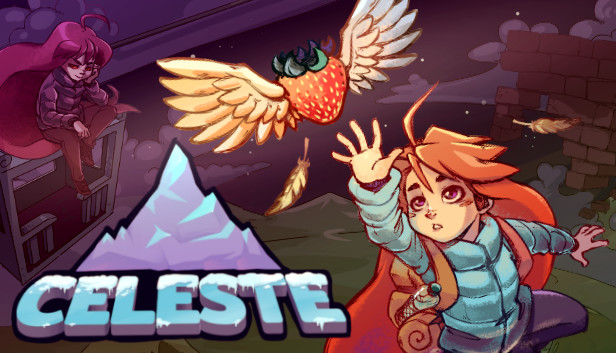
\includegraphics[scale=.5]{Imagenes videojuegos/Celeste.jpg}
    \caption{Imagen del videojuego Celeste}
    \label{img:featherCelesteA}
\end{figure}
\begin{figure}
  \centering
    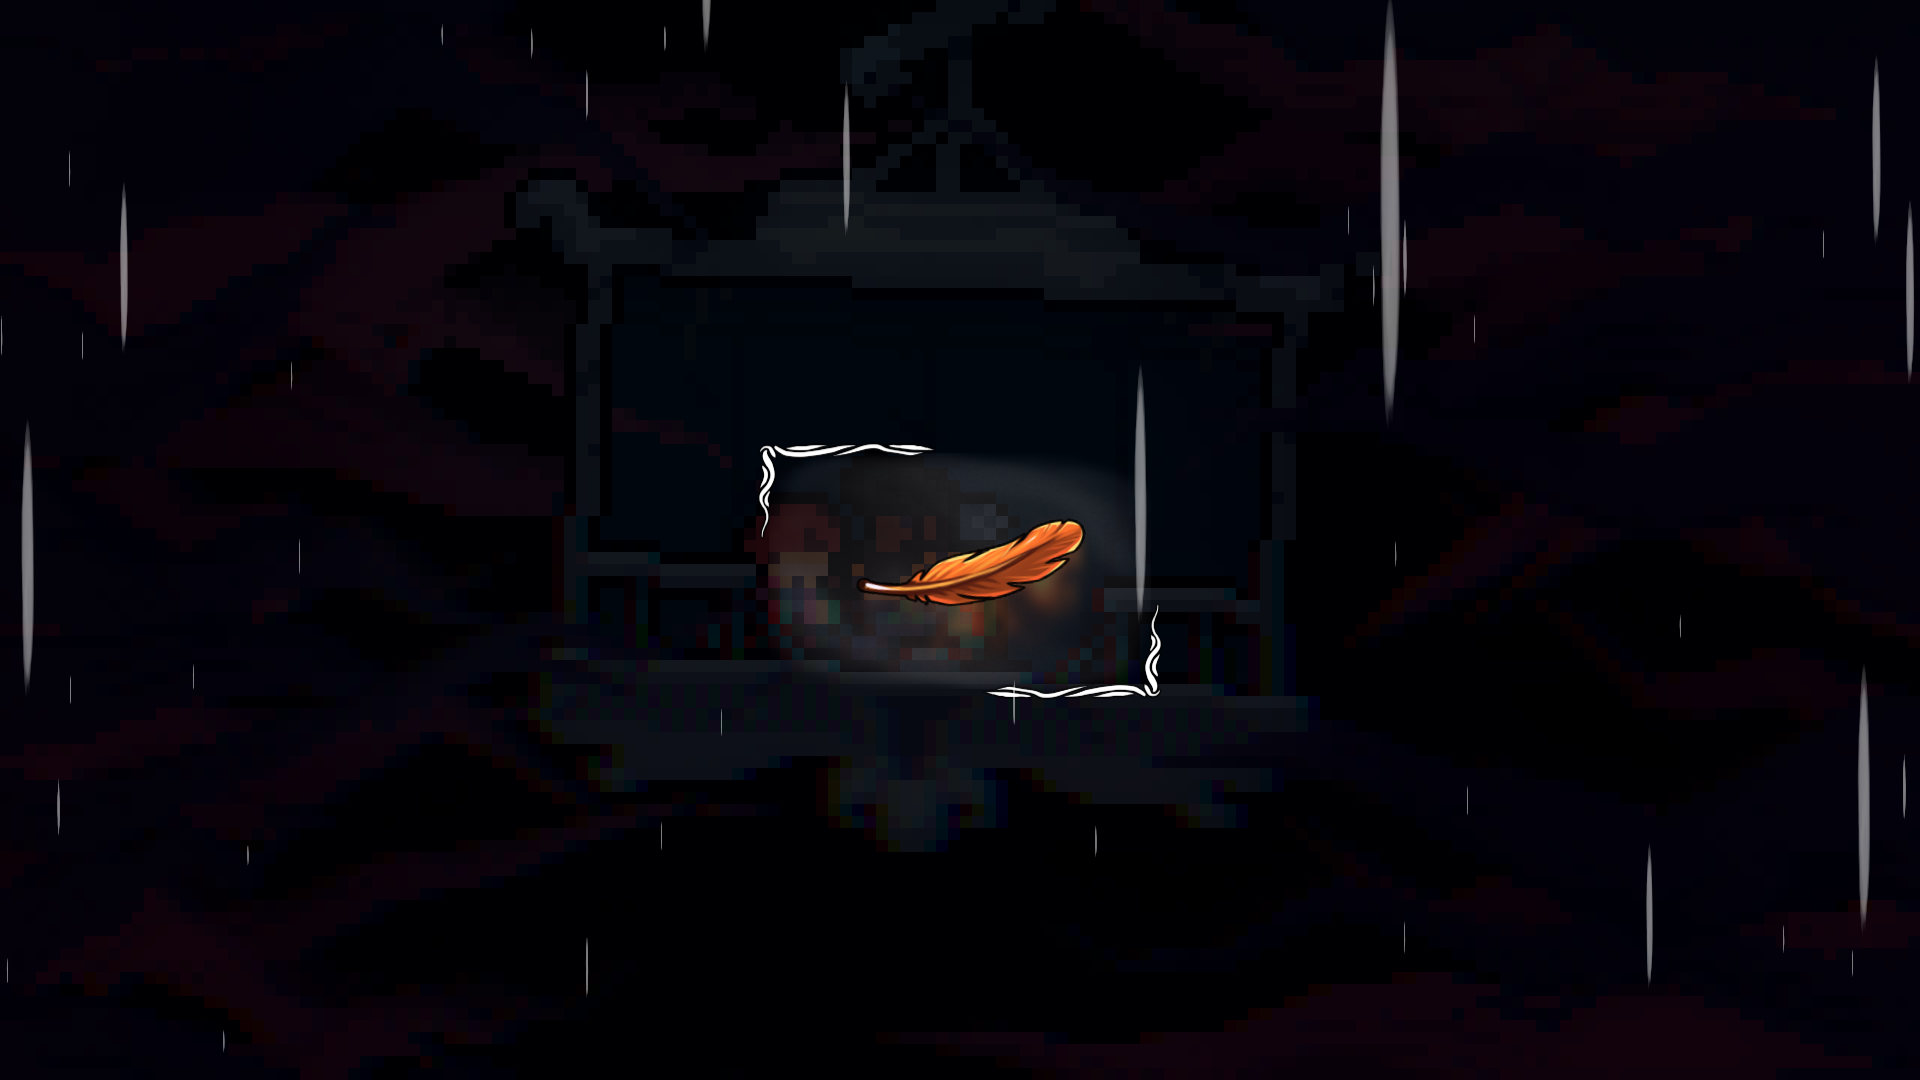
\includegraphics[scale=.2]{Imagenes videojuegos/featherceleste}
    \caption{Imagen del videojuego Celeste: minijuego de control de respiración}
    \label{img:featherCelesteB}
\end{figure}

Otro videojuego donde se representa claramente una enfermedad mental se trata de \citetitle{gris18} (véase imagen \ref{img:gris}), un juego realizado por el estudio catalán, \cite{nomadaStudio}. En este juego se representa la depresión por una pérdida, las recaídas que se sufren por el camino, la necesidad de ayuda. Todo esto lo hace, sobre todo, a través del arte, como puede verse en la imagen \ref{img:gris2}. Se comienza con la pérdida del color y voz, de lo que nace el nombre del juego. Estas propiedades se van recuperando a medida que se avanza en el juego, representando el proceso por el que está pasando el personaje y alguien que pueda sufrir estos problema. Al final del juego se puede ver cómo la curación comienza y la música vuelve a sonar más viva, vuelve la voz, se recuperan los colores, se abren las flores y consigue llegar al final. En este caso, a diferencia de \citetitle{celeste18}, no se puede morir, no hay vida ni nada que entorpezca la vista de los escenarios. Tampoco hay enemigos generalmente, a excepción de los jefes finales, la única meta es conseguir llegar al final y disfrutar del trayecto. 

\begin{figure}
	\centering
	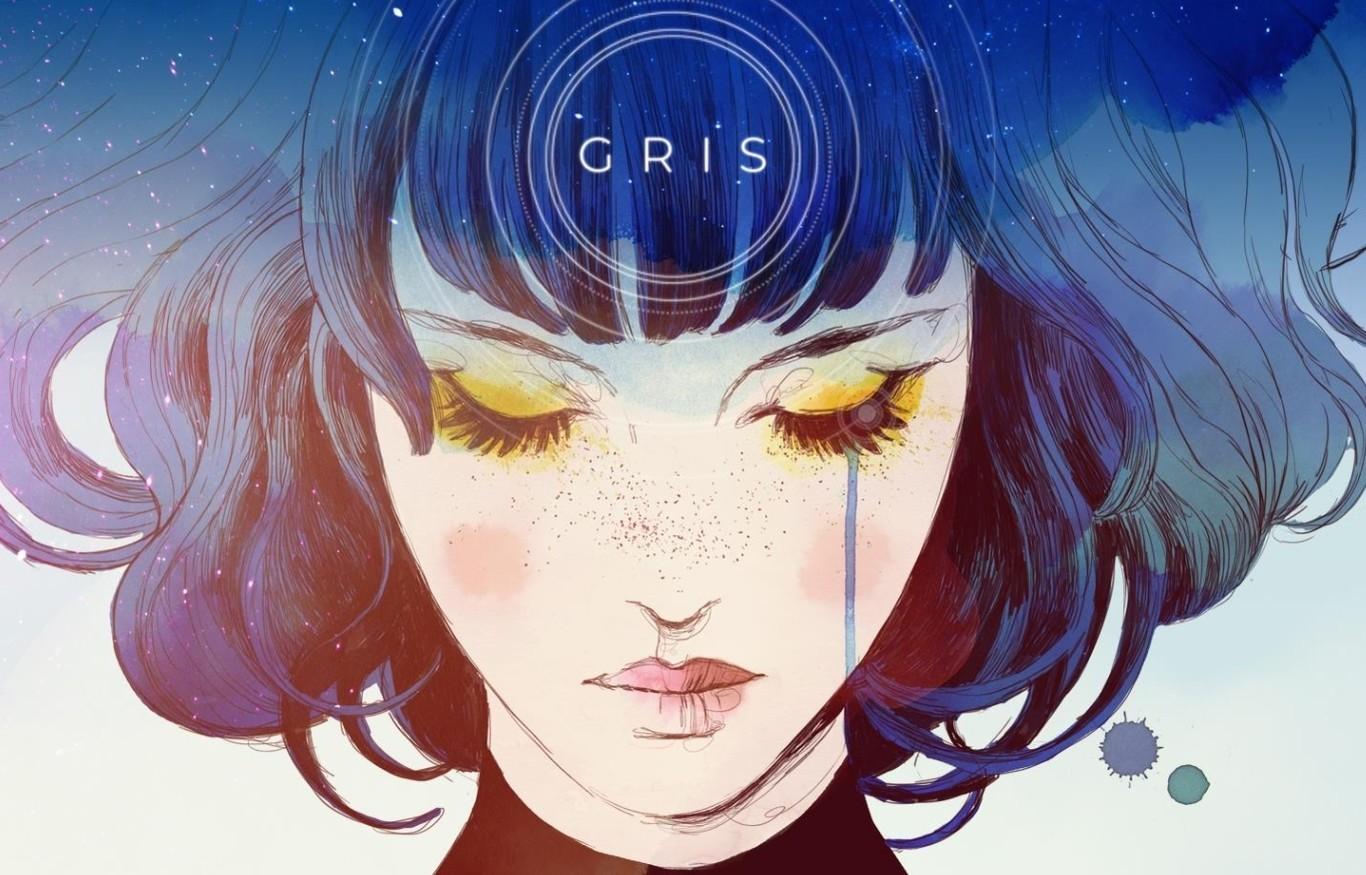
\includegraphics[scale=.4]{Imagenes videojuegos/gris.jpeg}
	\caption{Imagen del videojuego Gris}
	\label{img:gris}
\end{figure}
\begin{figure}
	\centering
	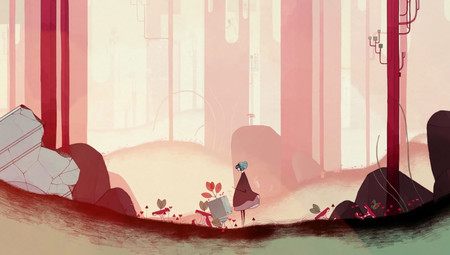
\includegraphics[scale=.7]{Imagenes videojuegos/gris2.jpg}
	\caption{Imagen del videojuego Gris in game}
	\label{img:gris2}
\end{figure}


En el artículo \textit{A Critique of GRIS} \cite{critiquegris}, el autor escribe \textit{ ‘GRIS’ is a beautifully depressing experience, one that combines entertaining puzzles into an ethereal platformer. It presents a masterclass in evocative romanticism of depression and death, one that could only work in a videogame. Hopefully, you can come to your own insightful conclusions about ‘GRIS’ and be moved as just as I was}. ('GRIS es una experiencia hermosamente deprimente que combina puzzles entretenidos en un plataformas etéreo. Presenta una masterclass en el romanticismo evocador de la depresión y la muerte, uno que sólo podría funcionar en un videojuego. Con suerte, podréis llegar a vuestras propias conclusiones sobre 'GRIS' y sentiros tan conmovidos como yo lo fui). 




Otro vidoejuego destacable es \citetitle{hellblade17}, (véase la figura \ref{fig:hellblade}), un juego considerado por los propios creadores como un indie triple-A, por el bajo presupuesto para el trabajo que requería, por tratar un tema que no suele estar tratado en los AAA,  por ofrecerlo al público a un precio también más reducido que lo que haría un AAA, y por tratar de cuidar la comunidad y tenerla cercana al desarrollo. 

En este videojuego se representa a Senua, una guerrera que debe llegar a su destino enfrentándose no sólo a los enemigos que encuentra por el camino, sino también a su propia cabeza. Senua sufre de psicosis, una enfermedad que hace escuchar voces continuamente, tener flashbacks, visiones que no sabe si son o no reales, pensamientos inmersivos, etc. 

En este caso, no sólo no sabe ella si todo esto es fruto de su cabeza o si son hechos reales, sino que tampoco el jugador sabe distinguir entre la realidad y el fruto de la enfermedad, haciendo que se sienta mucho más cercano a esta patología. Las voces se grabaron de forma que resonaran en los cascos de los jugadores para que sintieran también esta abrumación. Se utilizaba también como habilidad especial el reconocer patrones, que es algo que le ocurre a la gente que padece este tipo de enfermedad, de esta forma se completan algunos desafíos para seguir avanzando en la historia (veáse la figura \ref{fig:hellblade2}, donde se pueden ver los patrones observados). Las alucinaciones visuales y auditivas a veces sirven como guía para continuar con la historia. Esto fue criticado por algunos por tratar la enfermedad como un regalo o una ayuda. No obstante, esto no es siempre así, pese a que algunas alucinaciones sirvan como consejo o guía y otras muestren paisajes bonitos, en otras ocasiones se representa como una maldición. Esto lo hace con voces inmersivas, monstruos u oscuridad. 

Para realizar este videojuego y representar la enfermedad de la forma más fidedigna posible contaron con un equipo experto, entre los que se encuentra Fletcher, un profesor de neurociencia de la salud en la Universidad Cambridge y una serie de pacientes para que les explicaran cómo vivían ellos la enfermedad y mostrarles los avances y que dieran su opinión al respecto. Gracias a esto consiguieron hacer un juego con el que mucha gente que padece la enfermedad se sintiera realmente representados y pudiera utilizarlo para enseñar a su familia y su círculo cercano en cierto modo cómo era ser ellos y por lo que pasaban a diario. 

Además, este proyecto es interesante porque documentaron y publicaron buena parte del proceso de investigación y desarrollo del videojuego, las consultas con profesionales, pruebas con otros enfermos, cómo se hizo la creación del mundo, la captura del movimiento para ser trasladado a los modelos, etc. Todo esto puede verse en YouTube, en \citetitle{diariesprojecthellblade}. Remarcan además la importancia de recurrir a profesionales a la hora de tratar temas como las enfermedades mentales, para hacerlas lo más acordes con la realidad posible y tratando de no estigmatizarlas ni dañar al colectivo que las sufre. Este es un mensaje que se ha encontrado en otros tantos artículos, la necesidad de que, a la hora de tratar temas como la salud mental, se trabaje en común un equipo experto junto con el equipo de desarrollo.

En este caso, parece que hicieron un buen trabajo, pues recibieron una gran cantidad de mensajes por parte de la comunidad donde les daban las gracias por el trabajo realizado y cómo les había ayudado en su vida real para acercarles su enfermedad a su entorno. Les había ayudado a explicar cosas que nunca antes podían haber explicado o hecho sentir a sus allegados. En este otro vídeo (\citetitle{criticafanshellblade}) pueden leerse algunos de esos mensajes recibidos, entre los que se encuentran \textbf{\textit{'Your game made me cry because it showed me it was possible to undestand me'}} \textit{('Vuestro juego me hizo llorar porque me mostró que era posible entenderme')} o \textbf{\textit{'I had a psychotic break several years ago. My brother never understood. I overheard him say he was ashamed of me. After this game, he turned to me and said he was sorry. You got a message across that I never could'}} \textit{('Tuve un brote psicótico hace unos cuantos años. Mi hermano nunca lo entendió. Le escuché decir que estaba avergonzado de mí. Después de este juego, se volvió hacia mí y me pidió disculpas. Conseguísties mandar un mensaje que yo nunca pude')}. 


\begin{figure}
    \centering
    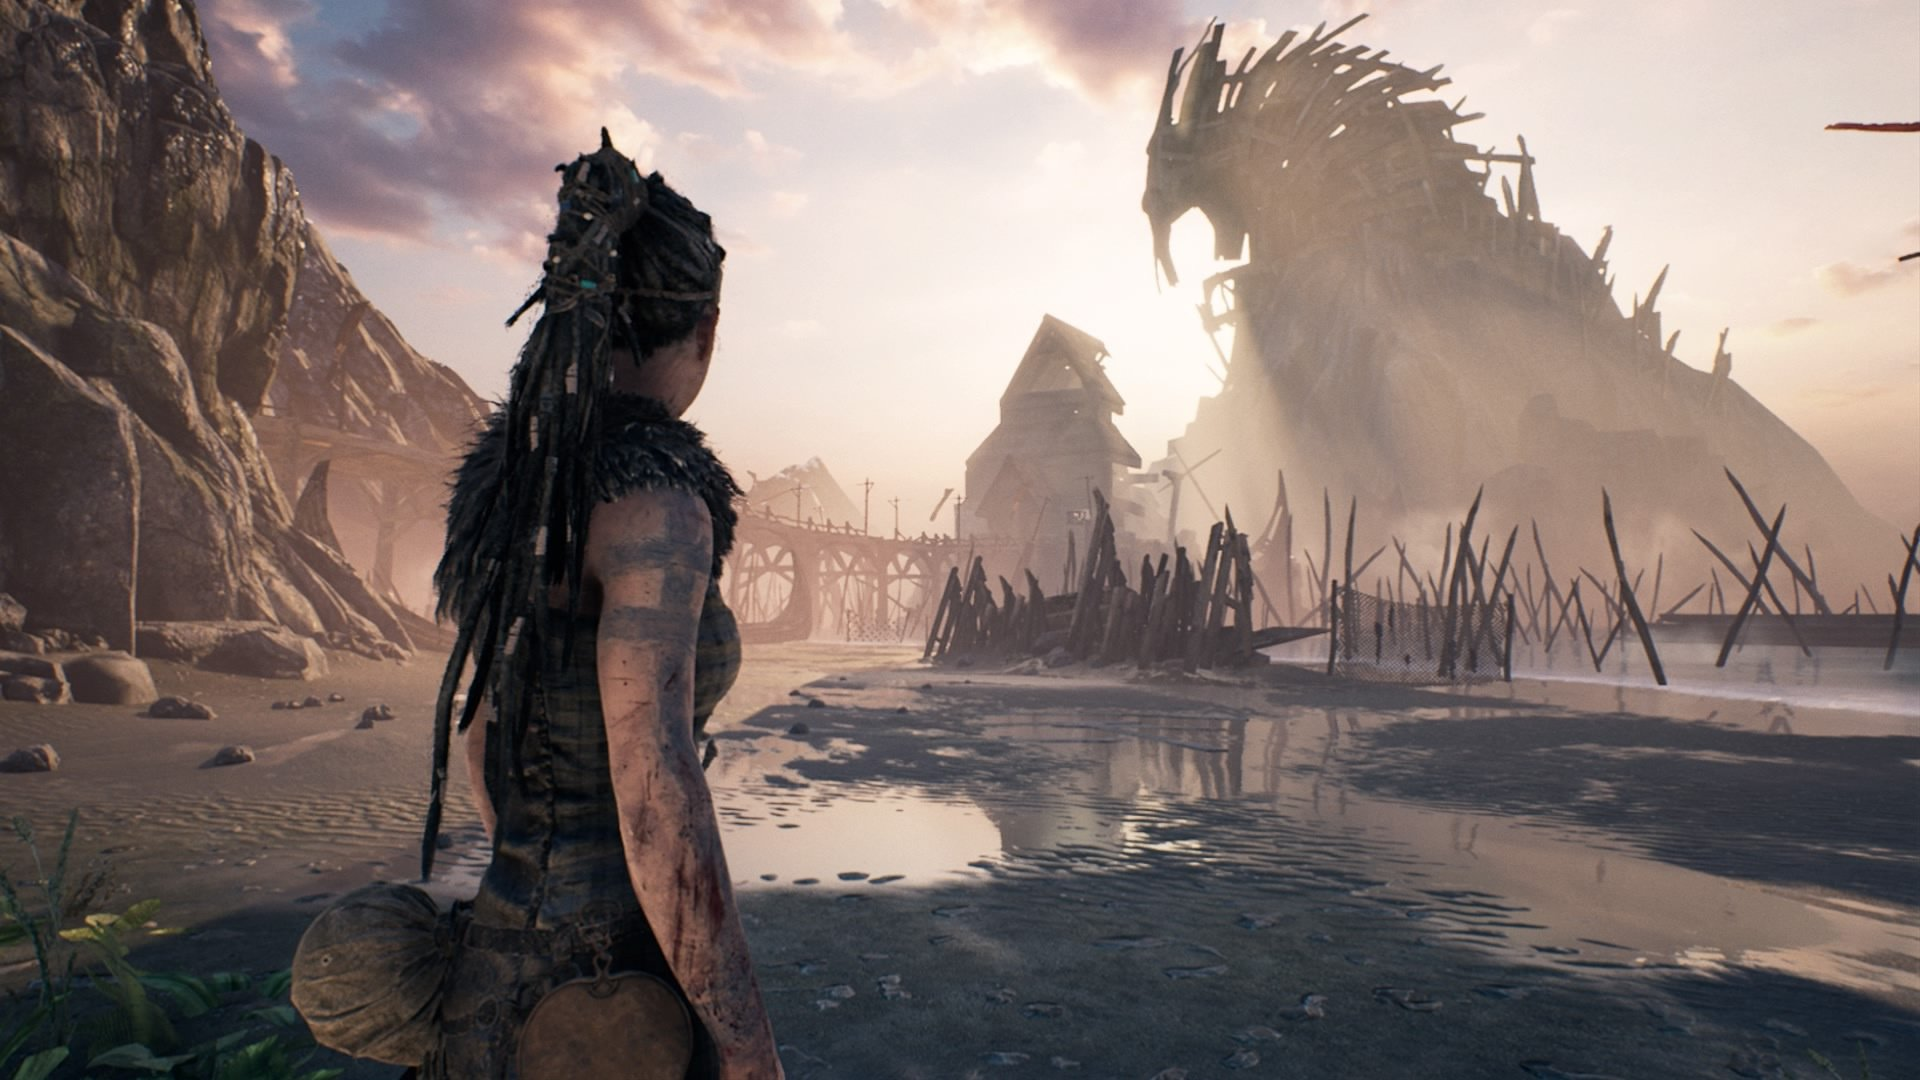
\includegraphics[width=.8\linewidth]{Imagenes videojuegos/hellblade.jpg}
    \caption{Captura del videojuego Hellblade: Senua's Sacrifice}
    \label{fig:hellblade}
\end{figure}
\begin{figure}
    \centering
    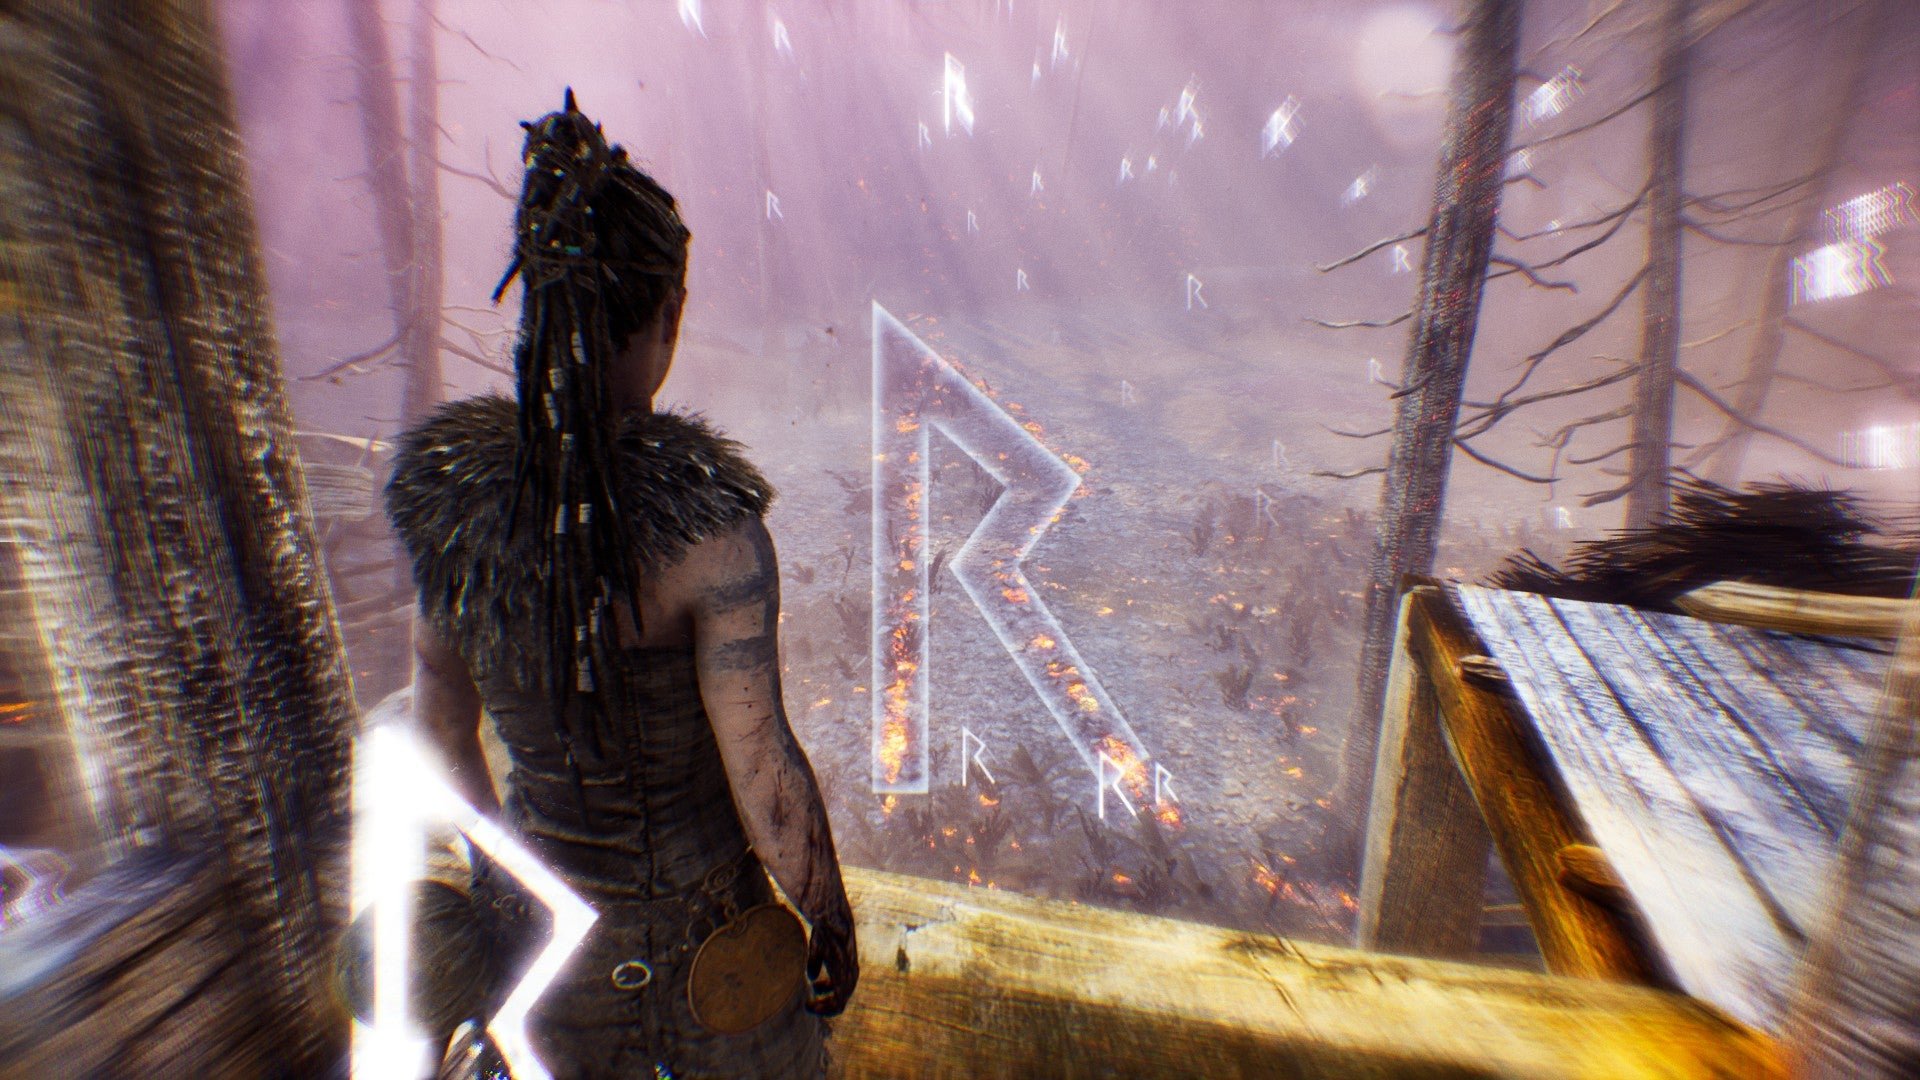
\includegraphics[width=.8\linewidth]{Imagenes videojuegos/hellblade2.jpg}
    \caption{Captura del videojuego Hellblade: Senua's Sacrifice; Patrones}
    \label{fig:hellblade2}
\end{figure}

\chapter{Metodología}


\begin{figure}
	\centering
	\includegraphics[width=1\linewidth]{TGF/Extra/Planificación.png}
	\caption{Planificación del TFG}
	\label{fig:planificacion}
\end{figure}


En primer lugar, la planificación seguida ha sido aproximadamente la siguiente \ref{fig:planificacion}. 

Se comenzó con la organización del trabajo, planteando qué se iba o no hacer y de qué manera. Se continuó con la investigación sobre el tema, se leyeron muchos artículos, tanto científicos como reportajes o artículos de opinión, así como valoraciones personales. Se vieron también vídeos de YouTube y demás recursos que trataran el tema del que se iba a hablar, la relación entre las enfermedades mentales y su representación en videojuegos o bien el efecto que tiene esta representación en quienes lo juegan. 

A continuación se comenzó con el análisis de la información recabada, que se puede consultar en la sección \ref{sec:estadoArte}. A la par, se creó la encuesta que posteriormente iba a compartirse por todos los medios posibles: familiares, redes sociales, amigos, etc. llegando a un total de 254 personas. Esta encuesta se creó tanto en castellano como en inglés, pudiendo llegar así a un mayor número de personas. Los resultados pueden consultarse en \ref{sec:encuestaVid} y en su totalidad en el anexo \ref{sec:anexo}. 

Con los datos recabados tanto en el análisis previo como en la encuesta, se empezó a diseñar y desarrollar un prototipo de videojuego que tratara ciertas enfermedades mentales. En este caso, habiendo comprobado la falta de representación que tenían algunas enfermedades y la cantidad de gente que las padece, se eligió representar un trastorno de la conducta alimentaria, un trastorno de ansiedad social y la depresión. El diseño de este prototipo, finalmente llamado ``Insania'', puede encontrarse en la sección \ref{sec:diseñoInsania}. 

Una vez creado un ejecutable jugable, se compartió con un equipo de probadores a los cuales se mandó una encuesta para la evaluación del mismo. Con los resultados obtenidos se modificó el prototipo corrigiendo los problemas encontrados así como aplicando las mejoras consideradas, como mayor solidez en los objetos que se estaban traspasando o añadiendo los controles de movimiento. El resultado de esta encuesta puede encontrarse en la sección \ref{sec:encuestaDemo} y en su totalidad en el anexo \ref{sec:anexo2}. 

Durante todo este tiempo se fue además documentando y creando esta misma memoria, creada con \LaTeX, para lo que se necesitó también cierto proceso de aprendizaje, al no haberlo utilizado con anterioridad. 



\section{Herramientas utilizadas}
En cuanto a las herramientas utilizadas, el proyecto ha sido realizado en Unity \cite{unity}, un motor de videojuegos multiplataforma creado por Unity Technologies. La programación que ofrece este entorno se realiza en C\#. La licencia utilizada ha sido Unity Education. 

Por otro lado se ha utilizado 3dsMax 2022 \cite{3dsmax} para la creación y modificación de algún modelo 3D. 3dsMax es un programa de Autodesk para la creación de gráficos y animación 3D. La licencia utilizada ha sido la educacional, que ofrece un año gratuito en el uso del software. 

Para la modificación de texturas, diseño gráfico de botones, pantallas, etc. se ha utilizado Adobe Photoshop \cite{photoshop}, herramienta de Adobe Systems Incorporated que se utiliza como editor de fotografías y gráficos. 

Como editor de audio se ha utilizado Audacity \cite{audacity}, un editor libre de derechos. 

Por otro lado, se ha utilizado \LaTeX para la creación de la memoria, \LaTeX es un sistema de composición de textos generalmente técnicos y científicos. La licencia es \LaTeX project public license. Para su uso se ha utilizado la herramienta Overleaf \cite{overleaf}, un editor de \LaTeX online propiedad de WriteLatex Limited, que permite trabajar en la nube, compartir documentos, etc. Se ha utilizado la versión gratuita. 

Llegando al final de la memoria, cuando ya pesaba mucho y tenía demasiadas imágenes y referencias, Overleaf dejó de ser útil pues la versión gratuita no permitía compilar archivos tan pesados. Por ese motivo, a partir de entonces se ha utilizado TeXstudio \cite{texstudio}. Un entorno de edición de \LaTeX de código abierto que tiene licencia GNU General Public License. 

Para las gráficas se ha hecho uso de Microsoft Excel \cite{excel}, software de hojas de cálculo propiedad de Microsoft, utilizado bajo la licencia educacional. 

En cuanto al resto de diagramas, se han realizado gracias a Creately \cite{creately}, una herramienta de creación de diagramas que ofrece todo tipo de plantillas y elementos para poder personalizar y crear desde diagramas UML a diagramas para brainstorming. Se ha utilizado la versión online y licencia básica. 

Durante la investigación se han utilizado tanto Adobe Acrobat Reader \cite{adobeacrobat}, como Weava \cite{weava}, una extensión de Google Chrome que permite subrayar y organizar páginas web y archivos PDF, crear citaciones automáticas, etc. (Ver Figura \ref{fig:weava}). 

\begin{figure}
    \centering
    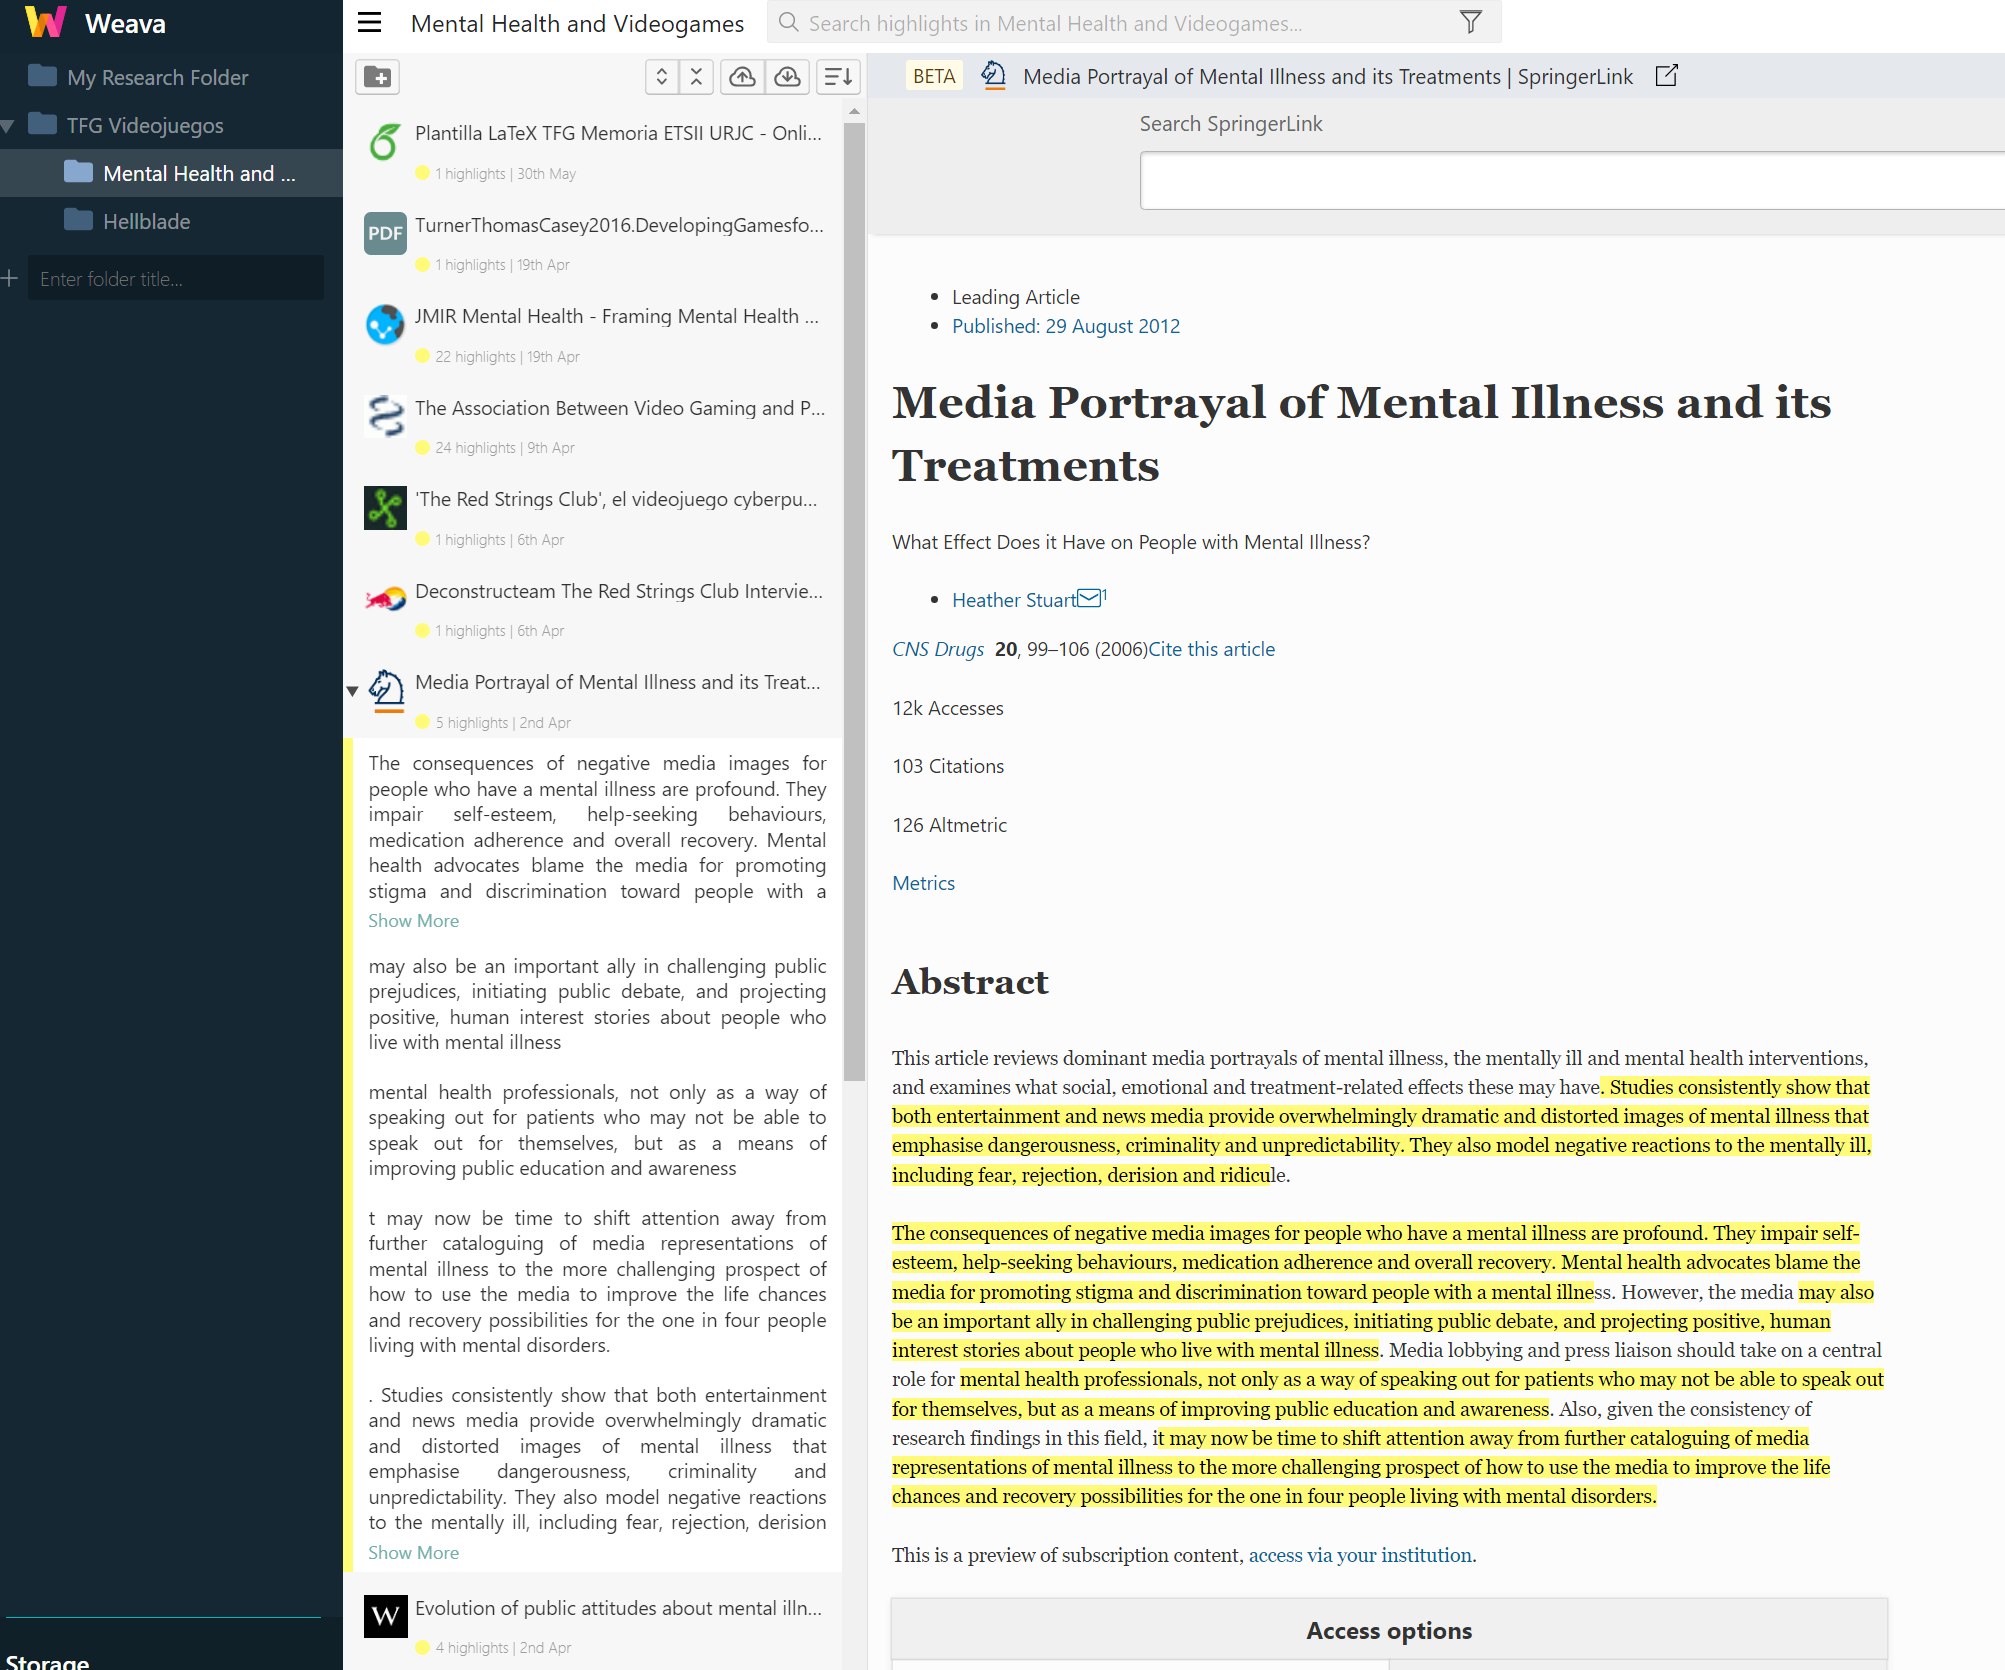
\includegraphics[width=.8\linewidth]{TGF/Extra/Weava.png}
    \caption{Ejemplo de la extensión Weava}
    \label{fig:weava}
\end{figure}



Para la recogida de información y organización se han utilizado tanto Google Docs \cite{googledocs} como Microsoft Word \cite{word}, en función de si se requería o no compartir la información online para poder tener colaboración e integración continua.

Con respecto a la integración continua en el proyecto, se ha hecho uso de Github \cite{github}, una herramienta de control de versiones, que hace uso de Git \cite{git}, donde se ha ido subiendo periódicamente el código y configuración del proyecto para que se tuviera acceso en todo momento. Se ha utilizado la versión de uso libre. 

Se ha utilizado Github Desktop \citetitle{githubdesk} para hacer las subidas a Github con un mayor control sobre los archivos que se subían, mayor facilidad a la hora de hacerlo, etc. 

Por último, para la búsqueda de recursos se ha utilizado Turbosquid \citetitle{turbo}, freepik \citetitle{freepik} y CGTrader \citetitle{CGTrader}, entre otros. 


\chapter{Diseño y desarrollo de ``Insania''}
\label{sec:diseñoInsania}
Gracias a la información recabada durante la investigación, que puede encontrarse tanto en la sección \ref{sec:estadoArte} como en la encuesta realizada que se puede encontrar en la sección \ref{sec:encuestaVid}, se ha diseñado y desarrollado un prototipo de videojuego que trata diferentes enfermedades mentales. 

En este prototipo, llamado ``Insania'', por su significado en latín, ``locura'', se podrá experimentar un poco cómo es vivir con determinados trastornos mentales, un trastorno de la conducta alimentaria, el trastorno de ansiedad social y la depresión. 

La finalidad es la representación y validación de las experiencias de estos personajes, de forma que los jugadores puedan sentirse identificados y, de ese modo, validados, por ellos mismos. En algunos casos puede ser duro enfrentarse a ciertos comentarios si se han llegado a tener o se tienen en algún momento, pero otras personas podrán considerar a estos personajes unos compañeros de batallas que pueden darles fuerza.

Se quiere, además, concienciar de que, pese a que no seamos psicólogos, podemos darnos cuenta de algunos detalles que pueden hacer saltar las alarmas y dar apoyo a quien creamos que puede estar pasando por algún mal momento. 

Es frecuente escuchar a la gente hacer comentarios sobre ``lo poco que come alguien'', escuchar un ``no voy a hablar por ti, si lo quieres, entra tú y lo pides'', cuando una persona probablemente tiene pánico a entrar en sitios con gente y hablar con desconocidos o ``pero por qué estás triste, si todo te va bien''. Invalidar los problemas de los demás o no percibir que algo puede estar pasando puede hacer que esos trastornos vayan a más y las personas se recluyan aún más y lo sufran en soledad al sentirse atacados ``en público''. 

Además, el problema muchas veces no viene simplemente de la falta de empatía o de querer hacer daño, viene de la falta de información, de no saber que ese comentario puede hacer sentir mal, de que, que una persona nunca quiera comer con gente puede significar algo más que ``que no tenga hambre''. Sin conocimiento se pueden decir muchas palabras dañinas sin saber que lo son, por eso cuanto más se hable de salud mental, mejor será para todos. 

\label{sec:diseño}
\section{Diseño general}
Partiendo del estudio previo realizado, analizando qué enfermedades se representan en videojuegos, de qué forma se hace y cómo es percibido por el público, tanto gente que las sufre como quienes no saben nada sobre ellas, se ha realizado un prototipo de videojuego, tratando de plasmar algunas de las enfermedades de las que menos se habla. Este prototipo será un juego en 3D realizado en Unity (versión 2021.1.0f1), pensado para ser jugado en PC, con los controles típicos de un juego de ordenador, donde se mueve el personaje con WASD o las flechas, se interactúa con la tecla del espacio y se accedé al menú de pausa con Esc. El target de este prototipo es para mayores de 12 años, por los temas que trata y la crudeza de algunos comentarios.  

En el prototipo se tratan tres enfermedades diferentes, y se muestra en cierta medida cómo es vivir con ellas. Estas enfermedades son un TCA (Trastorno de la Conducta Alimentaria), que, volviendo al estudio de videojuegos previamente realizado en la seccion \ref{sec:enfermedades}, sólo se mostraba en dos videojuegos, siendo uno de ellos esta misma demo y el otro, en \citetitle{darkest15}, donde los personajes pueden padecer bulimia, que les hace es recuperar menos vida cuando acampan. (\citetitle{darkest15} es un videojuego donde el jugador selecciona un grupo de personajes que deben ir de expedición a una mazmorra, en la cual se tienen que enfrentar a enemigos en un combate por turnos. Si la mazmorra es muy grande podrán descansar en un campamento donde pueden recuperar vida y cordura utilizando habilidades o comida, de ahí el hecho de que un personaje bulímico recupere menos vida en un campamento). Sin embargo no se trata la enfermedad como tal, sólo se hace un pequeño guiño. 

En el caso de la segunda enfermedad seleccionada, es el TAS (Trastorno de Ansiedad Social), enfermedad presente en tan sólo 4 de los videojuegos analizados, de nuevo siendo uno esta misma demo. Algunos de los videojuegos donde se representa son \citetitle{sym15} o \citetitle{lifeisstrange18}. Por ejemplo, \citetitle{sym15}, es un videojuego que explora la ansiedad social, representando al personaje en un laberinto dividido en dos submundos, uno que representa la vida normal y otro el lugar donde escapar de sus miedos. 

Por último, se ha escogido la depresión, en este caso no por la falta de representación, sino por lo frecuente que es esta enfermedad en la actualidad y de tan diversas formas. Haciendo referencia una de las encuestas realizadas en este trabajo, que se puede encontrar en \ref{sec:encuestaVid}, donde puede verse reflejado que un 24\% de las enfermedades mentales padecidas por los encuestados que padecen algún tipo de enfermedad mental son la depresión.

Las representaciones de la depresión suelen ser exageraciones de la realidad, de los síntomas, y de quienes lo padecen. Sin embargo, es una enfermedad que se sufre de muchas formas diferentes, y mucha gente la vive en silencio, sin saber que la padece, con mucho sufrimiento y sin pedir ningún tipo de ayuda, pues consideran que ``no están tan mal para tener depresión'', otros que ``eso es de flojos'' o incluso no consideran que sus problemas sean realmente importantes comparado con los de los demás y no tienen derecho a estar mal y quejarse. Mucha de esta gente acaba con tentativas de suicidio o sucumbiendo a él, y es por ello que ninguna representación es suficiente, y cuanta más representación y más diversa ésta sea, más gente se podrá ver reflejado y podrá entender qué le pasa y que la mejor solución es pedir ayuda y que no pasa nada por no estar bien y que se puede hablar de ello. 




\subsection{Personajes y trastornos}


El prototipo cuenta con tres personajes diferentes, cada uno de ellos seleccionable para disfrutar de una diferente experiencia de juego. Cada personaje padece un trastorno o enfermedad mental diferente, de forma que vivirán las situaciones que se le plantean y tendrá un comportamiento diferente teniendo esto en cuenta.  

\textbf{Personaje 1}: Este personaje padecerá un trastorno de la conducta alimentaria (TCA). Su diseño puede encontrarse en la sección \ref{sec:diseñoPersonajes}.

\begin{itemize}
    \item {\textbf{Descripción del trastorno:}   Estas enfermedades ``se caracterizan por una conducta alterada frente a la ingesta alimentaria o la aparición de conductas para controlar el peso'' \cite{tcasdescripcion}. Estos trastornos están relacionados, generalmente, con la autopercepción y la distorsión de la imagen corporal \cite{tcaCM}. Los diferentes tipos de trastornos de la conducta alimentaria son los siguientes: 
        \begin{itemize}
            \item {\textbf{Anorexia nerviosa:} se caracteriza por una restricción y reducción de la ingesta nutricional, que conduce a una pérdida significativa de peso. Existe un miedo por el aumento de peso y una imagen corporal muy distorsionada. En función del comportamiento seguido, existen dos tipos de anorexia nerviosa. En primer lugar, la anorexia nerviosa restrictiva utilizar como técnicas para la pérdida de peso la dieta, el ayuno y el ejercicio excesivo. Por otro lado, la anorexia nerviosa purgativa se caracteriza porque quien lo padece puede tener episodios recurrentes de atracones, de mucha o poca cantidad de comida, seguido de métodos purgativos (auto provocación del vómito o uso de diferentes tipos de laxantes o diuréticos). }
            \item {\textbf{Bulimia nerviosa:} se caracteriza por la existencia de atracones recurrentes, perdiendo el control sobre la ingesta. Para compensar este comportamiento, suele ir acompañado de la purga o excesivo ejercicio, para perder el peso ganado en esos atracones. En función de si existe o no purga se considerará ``bulimia nerviosa purgativa'', la persona utilizará para esa purga laxantes, diuréticos o provocación del vómito. En cuanto a la “bulimia nerviosa no purgativa”, se contrarrestan los atracones con un exceso de ejercicio físico y dietas.  }
            
            \item {\textbf{Trastorno por atracón:}  caracterizado por la existencia de atracones frecuentes, comer más rápido de lo normal, incluso sintiéndose lleno, comer mucho aun sin tener hambre, y sentirse por ello deprimido o con sensación de culpabilidad tras estos episodios. }    
             \item {\textbf{Trastorno restrictivo de la ingesta alimentaria:}  se caracteriza por una falta de interés en la comida, así como su evitación. En este caso, a diferencia de en los casos anteriores, no se produce por una preocupación por la imagen corporal y peso, no está afectado por la autopercepción sino por la propia comida y el miedo al atragantamiento o a las consecuencias de la acción de comer. Conlleva a una pérdida de peso, pese a no ser el objetivo buscado, y deficiencias nutricionales que pueden afectar al funcionamiento psicosocial.}
             \item {\textbf{Vigorexia o dismorfia muscular:}  pese a no ser considerado un trastorno de la conducta alimentaria, presenta algunas características comunes. Entre ellas se encuentran la preocupación excesiva por la imagen corporal, en este caso por encontrar su propio cuerpo pequeño o poco musculoso. Para solventarlo adquiere una serie de comportamientos compulsivos como la realización de una actividad física, dieta muy estricta, restrictiva y desequilibrada y a veces acompañada de otras sustancias como anabolizantes. } 
        \end{itemize}
    
    }
    \item {\textbf{Diagnóstico y comportamiento:}
     En este caso, el personaje padece de bulimia nerviosa no purgativa. Por el hecho de padecer este trastorno de la conducta alimentaria sufrirá un comportamiento compulsivo con la comida. Su preocupación por no ganar peso y no sentirse bien consigo mismo hará que sufra de atracones recurrentes, en los que perderá completamente el control sobre lo que ingiere. A consecuencia de esto, el sentimiento de culpabilidad y tristeza hará que adopte ayunos y dietas estrictas, así como un exceso de ejercicio físico. Tendrá problemas para comer en público o estando con personas, al sentir la mirada de todo el mundo, tener miedo a que los demás piensen que come mucho, que juzguen su imagen corporal, etc.  
     }
    \item {\textbf{Trasfondo:}
    Este comportamiento comenzó hace alrededor de dos años con la intención de hacer una dieta para bajar un par de kilos. Sin embargo, no tuvo ningún tipo de seguimiento ni recomendación por ningún personal cualificado, lo cual hizo que se empezara a obsesionar con la ingesta de calorías. Cuando la dieta “finalizó”, dos meses después de su comienzo, volvió a la alimentación anterior, lo cual le hizo ganar aún más peso del que partía.
    
    A raíz de este suceso perdió el control con la comida, encontró en ella un escape para sus frustraciones y malestar. Tras estos atracones sentía un gran sentimiento de culpa por lo que volvía a empezar una dieta no demasiado restrictiva. Poco a poco la obsesión fue empeorando y en lugar de dietas no restrictivas, algunos días su sentimiento de culpa era tan grande que entendía que sólo el ayuno podía compensar el atracón. Desde entonces continúa con este problema, cualquier hecho estresante o problema, acaba reflejado en la comida con una gran ingesta de todo tipo de comida. Tras eso tiene un período de dieta estricta, ayuno y ejercicio excesivo. Además, esto ha afectado también a sus relaciones sociales, pues no puede comer en presencia de nadie más, tiene una relación muy mala con la comida y trata de ocultarlo a su alrededor. Sin embargo, el hecho de no comer en público resulta un comportamiento extraño para su alrededor, que, en vez de tratar de entender lo que le ocurre y apoyarla, sólo aportan comentarios que hacen que se sienta peor, en los que no dejan de comentar que ``no come nada'', ``está en los huesos'', o bien que ``para no comer tampoco está tan delgada''. 
    
    De momento ha dado el paso a reconocer que tiene una enfermedad que se ha auto diagnosticado, dado el comportamiento que se ha dado cuenta que tiene y que no es normal. El siguiente paso que quiere dar es pedir ayuda y contárselo a su familia o bien acudir a terapia. Todavía no está preparada para ninguna de ambas cosas, pero considera que, de momento, al haberse dado cuenta, lo tiene más o menos controlado, pese a que no sea el caso.
    }
    
      \item {\textbf{Decisiones sobre el personaje:}
     En este caso se ha escogido un personaje de género femenino dado que, tal y como muestran los estudios realizados al respecto, son las mujeres las que presentan una mayor prevalencia de la enfermedad. 
     
     Como puede verse en un artículo \cite{articuloTCA}, que recoge a su vez estudios epidemiológicos sobre trastornos de la conducta alimentaria realizados en España a lo largo de los años, todos ellos coinciden en que la prevalencia es mayor en mujeres que en hombres, encontrándose los valores entre un 3,4-7,7\% de prevalencia entre mujeres y de un 0,2-1,7\% en hombres. Otros artículos \cite{articuloTCA2} incluso estiman que son las mujeres las que, en un 90\%, padecen este tipo de enfermedades. Además, generalmente adolescentes y jóvenes. En concreto, la bulimia nerviosa, está estimado que afecta a de una a tres mujeres por cada 100. Los hombres, sin embargo, tienen una proporción diez veces menor. 
     
     También en la encuesta realizada, que se puede encontrar en la sección \ref{sec:encuestaVid} y más claramente en el anexo \ref{sec:anexo}, puede observarse que de entre todas las enfermedades padecidas por mujeres y hombres, los TCA suponen un 10\% del total, mientras que en el caso de los hombres este porcentaje desciende a un 2\%. 
     
    Esto se intenta explicar tanto por implicaciones culturales como, según algunos estudios, como el siguiente \cite{articuloTCA3}, por factores genéticos. Es indudable que la cultura promociona un ideal de cuerpo delgado al que tratan de aspirar las mujeres, sobre todo adolescentes que se encuentran en la pubertad y empiezan a ver cambios en su cuerpo, ensanchamiento de caderas, mayor cantidad de grasa corporal, etc. Además, el factor cultural es muy importante, sobre todo en la era de la tecnología, donde incluso Instagram tuvo que pedir disculpas y añadir nuevas restricciones en 2019 para no mostrar según qué publicaciones a menores de edad, así como eliminar ese tipo de publicaciones de los algoritmos de recomendación \cite{articuloTCA4}. No prohíbe exponer las experiencias personales pero sí el contenido que incita a tener este tipo de trastornos. Además intentan que no se viralicen los contenidos relacionados o que puedan llegar a los ojos de gente vulnerable, bien por su minoría de edad, bien por estar pasando por el mismo proceso, o por estar en recuperación. 
    
    En cuanto a la selección de esta enfermedad, como se ha podido ver a lo largo del trabajo, donde se exponen diferentes juegos que reflejan distintos tipos de enfermedades o trastornos mentales, prácticamente ninguno de ellos muestra este trastorno. Para ser una enfermedad que afecta a tanto porcentaje de la población (alrededor de un 9\% de la población de EEUU tendrá un trastorno alimenticio a lo largo de su vida, según la ANAD \cite{articuloTCA5}, no está representada como debería. La poca representación que hay tampoco es fidedigna, se suelen mostrar cuerpos esqueléticos, centrándose únicamente en el aspecto físico de la enfermedad y exagerando unas características que no todo el mundo que padece esta enfermedad posee. De hecho, según estudios, menos del 6\% de la gente diagnosticada con un trastorno de la conducta alimentaria está considerada como que tiene bajo peso. 
    
    Además, el TCA es una de las enfermedades mentales más mortales, la segunda, después de la sobredosis por opiáceos, 10200 muertes cada año son causa directa de un trastorno de la conducta alimentaria. No solo eso, sino que un 26\% de las personas que padecen estos trastornos sufre intentos de suicidio, como se puede ver en los artículos siguientes \cite{articuloTCA6} y \cite{articuloTCA7}. 
    
    Como puede verse por los datos ofrecidos, es una enfermedad demasiado relevante para tener tan poca representación e información sobre ella. Esto sólo puede cambiarse creando nuevos contenidos que ofrezcan esa realidad desde diferentes puntos de vista, desde diferentes medios. 
    
    Con respecto a los videojuegos, sólo ocho videojuegos en la plataforma itch.io están categorizados con la etiqueta “eating disorders”. En cuanto a series y películas, existe alguna película y serie que trata el tema, como \citetitle{tothebone} o \citetitle{feed}, y otras series tienen personajes que padecen este tipo de trastornos. Sin embargo, como mencionaba anteriormente, la mayoría de ellos perpetúa una imagen irreal sobre la enfermedad y no las reflejan como son, confundiendo anorexia con bulimia, y viceversa. Se enseña a la población que lo consume que la anorexia supone una restricción en la ingesta y la bulimia, purgación. Tal y como se ha explicado antes, esto no es necesariamente así, existen diferentes tipos de anorexia y bulimia, y la diferencia entre estas dos enfermedades no reside en cómo “no ganar peso”, sino en la relación con la comida y qué provoca el trastorno. 
    
    Con este personaje y la situación que se plantea con él se pretende mostrar un nuevo punto de vista, una nueva perspectiva sobre la enfermedad, no centrada en el peso ni en la comida, sino en lo que pasa en la mente de las personas con estos trastornos. La necesidad de control, de perfección, y el sentimiento de culpa al sucumbir al descontrol, sobre todo con la ingesta calórica. 
    
    Además, se pretende dar a la enfermedad la importancia que tiene e intentar mostrar algunos comportamientos para favorecer su detección, tanto en uno mismo como en los demás. Generalmente sólo se presta atención o “detecta” cuando se llega a niveles de infrapeso y la apariencia física es claramente diferente, no teniendo en cuenta que hay trastornos que son igual de dañinos pese a que no se llegue a esos niveles de infrapeso, como suele ocurrir con el trastorno por atracón, o incluso con la bulimia. También se quiere hacer hincapié en que los comentarios sobre el aspecto físico de los demás no deberían ofrecerse a no ser que sean preguntados. Ni para comentar un aumento de peso ni para felicitar por una pérdida del mismo, pues no se sabe las razones que han llevado a ese punto y felicitar a alguien que padece un trastorno de la conducta alimentaria centrada en la pérdida de peso sólo va a perpetuar la enfermedad. }

\end{itemize}



\textbf{Personaje 2}: Este personaje padecerá un trastorno de ansiedad social (TAS). Su diseño puede encontrarse en la sección \ref{sec:diseñoPersonajes}.

\begin{itemize}
    \item {\textbf{Descripción del trastorno:}
     El trastorno de la ansiedad social se caracteriza por un miedo irracional y persistente a las situaciones sociales por temor a que resulten embarazosas. Existen diferentes escalas para evaluar la gravedad de este tipo de ansiedad. Las situaciones más frecuentes en las que se pone de manifiesto este trastorno son al hablar en público, reuniones sociales o encuentros inesperados. Pueden desencadenar síntomas físicos como la sudoración excesiva, ruborización, palpitaciones, temblor, tartamudez e incluso desembocar en ataques de pánico. 
     
     Se considera un extremo patológico de la timidez, que supone una evitación de las situaciones que pueden suponer este malestar. Además, se suelen utilizar diferentes “conductas de seguridad” para sobrellevar esta sintomatología como puede ser evitación de mirada, de acudir a ciertos lugares o encontrarse con personas, adquirir una postura defensiva con los brazos cruzados, las manos en los bolsillos o detrás de la espalda o bien jugar con las manos, estrujarlas, juntarlas, soltarlas, etc. También entran entre estas conductas revisar y evaluar el discurso antes de realizarlo de forma compulsiva, manipular objetos para calmar la ansiedad, o dejar de realizar acciones cuando se siente la atención de alguien o alguien se acerca. Otras técnicas de evitación consisten en la ingesta de alcohol, ansiolíticos u otro tipo de drogas para conseguir el efecto desinhibidor.  
     
     El padecimiento de esta enfermedad puede desencadenar problemas mayores como peor rendimiento en el colegio/instituto/universidad, al tender a evitar atender a clase, problemas en el trabajo por una peor productividad o consecutivas ausencias. Además, hay riesgo de sufrir un abuso de alcohol y drogas, excesiva soledad o pensamientos suicidas. 
    }
    \item {\textbf{Diagnóstico y comportamiento:}
     En este caso el personaje tratará de evitar las situaciones en las que esté con gente, sobre todo si hay más de una persona. En esas situaciones sentirá que tiene todos los ojos posados en su persona y tendrá miedo de hacer el ridículo, sentirá sensación de agobio y tendrá tendencia a ocultarse, no llamar la atención y prepararse la interacción con otras personas en el caso de ser inevitables. Además, una vez finalizada esta interacción se cuestionará su comportamiento y castigará, teniendo miedo de haber hecho el ridículo, pensando cómo debería haber actuado en su lugar, etc.   
     }
    \item {\textbf{Trasfondo:}
    Desde que era pequeño en su familia de tres hermanos él era siempre considerado el tímido. Cuando se le presentaba a alguien se ponía fijación en esa característica: “nunca habla”, “uy, por favor, decidle que se calle que me tiene la cabeza loca”. A pesar de ser un rasgo de su personalidad, acabó convirtiéndose en un papel que tenía que cumplir siempre, si no quería recibir comentarios de naturaleza contraria “pero bueno, qué haces tú hablando”, “anda, si tiene lengua”, que únicamente le hacían sentir peor dada su timidez y su aversión a llamar la atención. 
    
    Al final el papel acabó comiéndose a la persona, de modo que nunca más se planteó ser de otra forma. Además, poco a poco se fue transformando en un problema, pues ya no simplemente no hablaba cuando estaba con gente extraña, sino que empezó a tener problemas para participar en clase. Salir a la pizarra se convirtió en una de sus peores pesadillas. Nunca recibió bullying por parte de sus compañeros, pero él mismo en su cabeza pensaba que todos estarían criticándole, pensando mal de él, no quería ser el centro de atención. Comenzó con sudores cuando le tocaba salir y un poco de malestar, y se acabó convirtiendo en un trauma, tenía pesadillas por las noches y dejó de querer ir a clase por lo mal que lo pasaba en esos momentos. 
    
    Pese a ello, siguió haciéndolo y cuando vio que en secundaria ya no le sacaban a la pizarra por ser una de las personas con mejor rendimiento académico, se relajó. Su problema, sin embargo, se trasladó a otros lugares, no podía comer en el comedor, le costaba horrores ir a un establecimiento y entablar conversación con el dependiente, prescindía de asistir a todo tipo de fiestas y reuniones para evitar estar con mucha gente y cuando lo hacía entraba en pánico, lo cual trataba de controlar quedándose en alguna esquina y jugando con sus manos para calmar la ansiedad hasta que todo acababa. 
    
    Actualmente sigue lidiando con todos estos problemas y no se ha planteado buscar ayuda al considerar que lo que tiene es una tontería y que simplemente tiene que dejarse de tonterías y madurar. Cuando se encuentra con alguna de las situaciones que le provoca malestar, primero trata de cancelarlas o evitarlas, y en el caso de no poder, intenta controlar sus síntomas y malestar buscando entretenimientos, como puede ser mirar el móvil o ponerse música. 
    
    Sin embargo, desde un tiempo para atrás, esta sintomatología está viéndose incrementada por el estrés de su situación personal, lo cual le hace que sea más difícil controlar el pánico en esos momentos, llegando a tener el otro día un ataque de pánico en la universidad, en medio de una clase. Esto ha hecho que tenga aún más miedo a enfrentarse a estas situaciones porque ya ni siquiera tiene la sensación de poder controlarlas. 
    }
    
     \item {\textbf{Decisiones sobre el personaje:}
     En el caso del TAS, es una enfermedad que se considera que tiene una prevalencia general de alrededor de un 12\% \cite{articuloTAS}. Este mismo estudio determina que hay una mayor prevalencia en mujeres que en hombres, pese a que los resultados no sean los mismos en todos los estudios realizados y diferencia las situaciones más frecuentes en las que lo sufren mujeres y hombres. 
     
     En la encuesta realizada, que se puede encontrar en la sección \ref{sec:encuestaVid} y más extensamente en el anexo \ref{sec:anexo}, puede verse que el TAS supone un 10\% del total de enfermedades padecidas por personas de género femenino y sin embargo un 18\% en el caso de personas de género masculino y un 16\% en el caso de las personas de género no binario. Por este motivo, en este caso se ha escogido la representación en una persona de género masculino. 
     
     
En cuanto a las situaciones en las que sienten más miedo hombres y mujeres, en principio las mujeres tienen más miedo en situaciones profesionales, como entrevistas, hablar a figuras de autoridad o hablar en público, mientras que los hombres solían sufrir más miedo en citas, fiestas o encuentros sociales. (Ver figura \ref{fig:TAS})

\begin{figure}
    \centering
    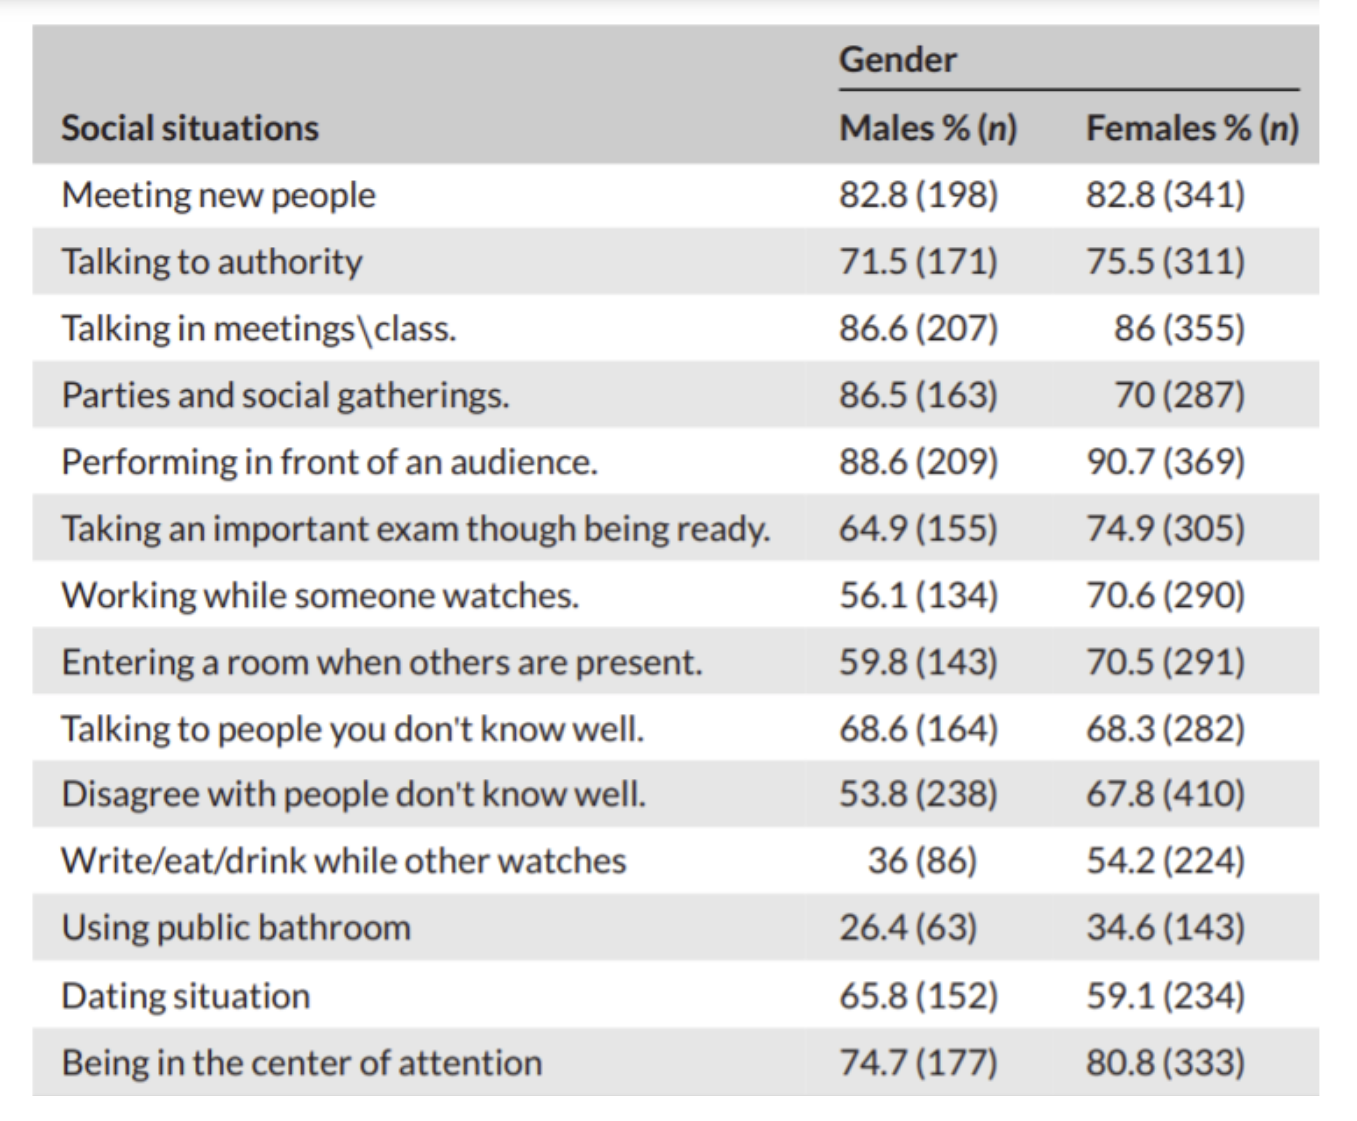
\includegraphics[width=.9\linewidth]{TGF/Extra/TAS.png}
    \caption{Situaciones sociales de mayor miedo por géneros}
    \label{fig:TAS}
\end{figure}

\begin{figure}
	\centering
	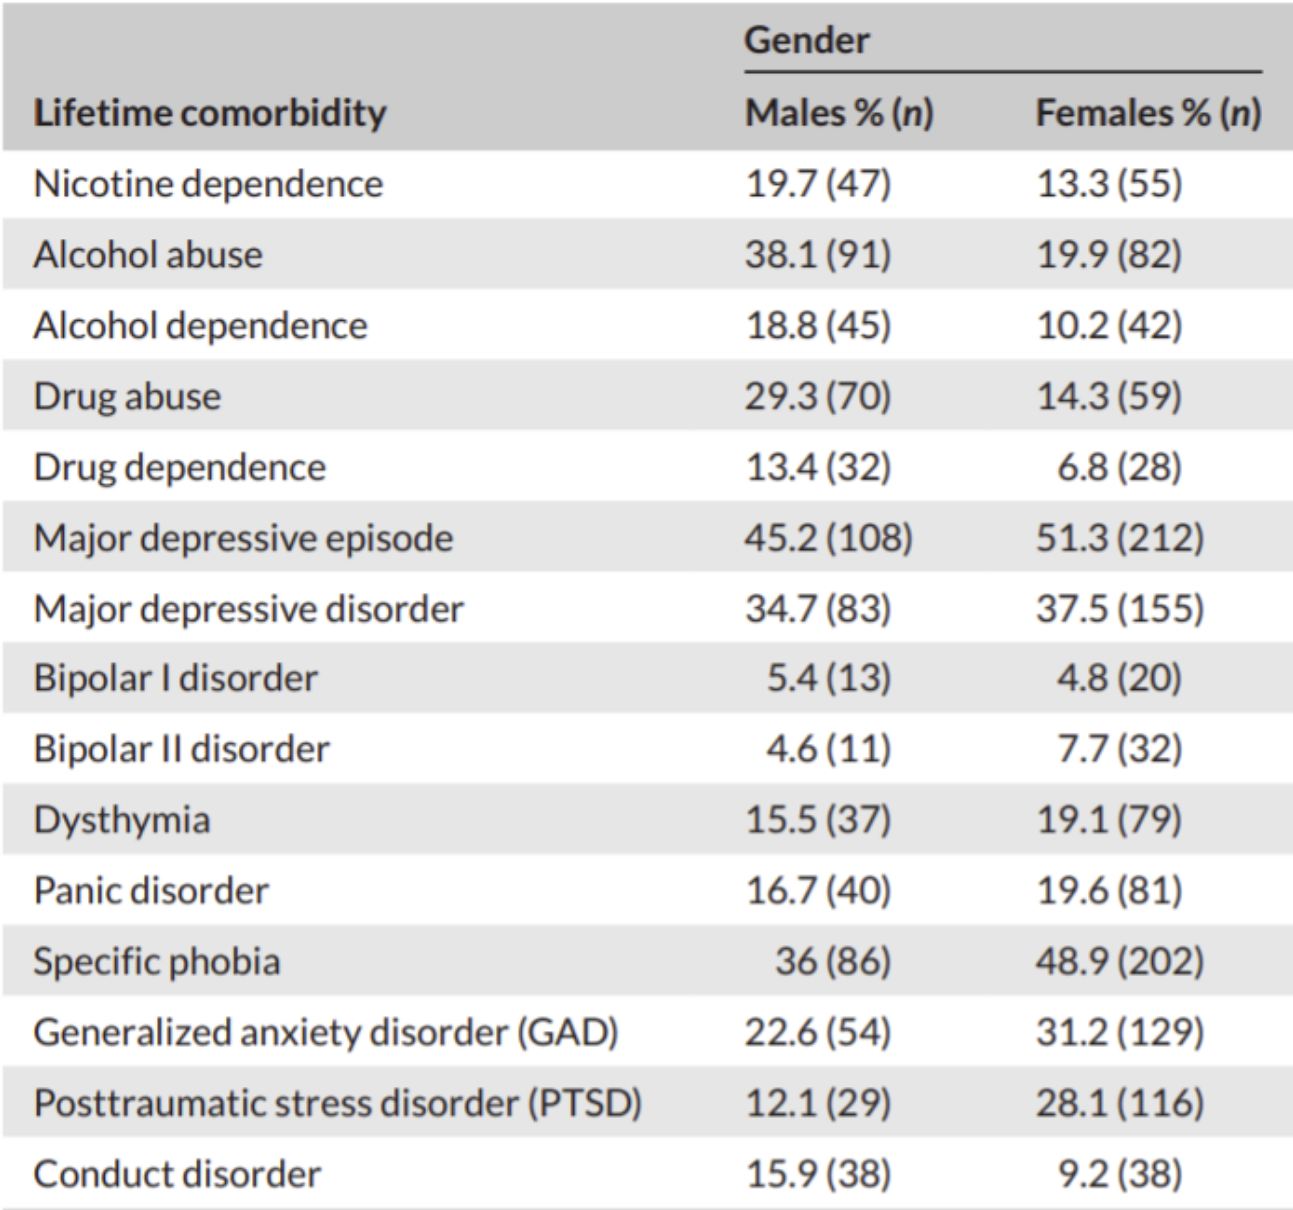
\includegraphics[width=.9\linewidth]{TGF/Extra/TAS2.png}
	\caption{Presencia de otros trastornos, además del TAS, por géneros}
	\label{fig:TAS2}
\end{figure}


Además es diferente la forma de lidiar con ello o las enfermedades que desencadenan, siendo más frecuente en hombres sufrir de abuso y dependencia de alcohol y drogas, así como problemas de conducta, mientras que en las mujeres está más relacionado con el estrés post traumátrico, la ansiedad generalizada, y trastornos o episodios depresivos, así como fobias específicas. (Ver figura \ref{fig:TAS2}).

Se coincide además en que las personas que sufren este tipo de trastorno son de las que menos buscan ayuda de entre todos los que padecen algún trastorno de ansiedad \cite{articuloTAS2}, debido a la timidez o vergüenza que suele ir ligada a la ansiedad social. De ese modo, tratan de esconder esos problemas e intentar lidiar con ellos de forma autónoma, menospreciando la validez o importancia del problema. 

Como se ha mencionado anteriormente, diferentes estudios muestran diferentes resultados con respecto a la prevalencia de la enfermedad en mujeres u hombres. En \citetitle{elmio} se ha optado por mostrar la enfermedad desde el punto de vista de un personaje de género masculino, por la encuesta realizada. Sin embargo, en este caso no está relacionado con los aspectos más comunes en los hombres, no hay abuso ni dependencia del alcohol y drogas ni trastorno de la conducta.  


Al enseñar este trastorno se pretende dar visibilidad al sufrimiento de muchas personas que suele considerarse una tontería o cosas de niños, cuando realmente es un problema y el que lo sufre lo pasa mal y tiene una enfermedad que probablemente no pueda superar sólo, necesita apoyo y, en muchos casos, ayuda profesional.
}
     
\end{itemize}




\textbf{Personaje 3}: Este personaje padecerá depresión. Su diseño puede encontrarse en la sección \ref{sec:diseñoPersonajes}.

\begin{itemize}
    \item {\textbf{Descripción del trastorno:}
     La depresión es un trastorno del estado del ánimo, transitorio o permanente, que se caracteriza por un sentimiento de tristeza o pérdida de interés en realizar cualquier tipo de actividad. Existe la posibilidad de tener dificultad incluso para realizar las actividades cotidianas. Entre los síntomas, se encuentran una gran cantidad y variedad de ellos, pese a que no tengan por qué sufrirse todos ellos. 
     
     Algunos de esos síntomas son el sentimiento de tristeza o vacío, pérdida de interés en cualquier tipo de actividad, alteraciones del sueño, cansancio y falta de energía, trastornos en la conducta alimentaria, bien por la falta del apetito o por los antojos de comida, que suponen una pérdida o ganancia de peso. También puede sentirse ansiedad (de hecho, es típico sufrir de este trastorno junto con el trastorno de ansiedad generalizada), dificultad de concentración o en la toma de decisiones, dolores físicos, e incluso pensamientos o intentos suicidas.
     
     Es una enfermedad que, además, suele presentarse con una frecuencia que es casi el doble en el caso de las mujeres que en el de los hombres. 
     
     
     Existen diferentes tipos de depresión, entre ellas se encuentran: 
         \begin{itemize}
            \item {\textbf{Trastorno depresivo mayor:} previo a este episodio pueden experimentarse otros síntomas como la ansiedad, fobias, o ataques de pánico. En función de si existe un único episodio o más, se considerará, ``trastorno depresivo mayor de episodio único'', o bien ``trastorno depresivo mayor recurrente''. Se caracteriza por la presencia de algunos o todos los siguientes síntomas durante, al menos, dos semanas:  un bajo estado de ánimo durante la mayor parte del día y de los días, pérdida o aumento del apetito, disminución de la capacidad de disfrute, sensación de debilidad, sentimientos de inutilidad o culpa, insomnio o hipersomnio (dormir más o menos de lo habitual), etc. }
            \item {\textbf{Trastorno distímico:} los criterios o síntomas son similares al caso anterior, con la mayor diferencia de que se poseen durante un mínimo de dos años, pudiendo no existir alguno de ellos durante no más de dos meses seguidos. Además, se considera este tipo de trastorno si no existen antecedentes de otras enfermedades o se presentan los criterios de otras enfermedades como trastorno bipolar, esquizofrenia, etc.}
            \item {\textbf{Trastorno adaptativo o depresión reactiva (ansiedad y ánimo depresivo:} la aparición de la sintomatología suele venir en respuesta a un acontecimiento estresante, siendo esta respuesta “desproporcionada” para ese factor estresante. }    
             \item {\textbf{Trastorno depresivo no especificado: }  se considerará aquella situación en la que se presentan algunos de los síntomas depresivos, pero no suficientes para el diagnóstico de ninguno de los otros trastornos. A veces por el solapamiento con un trastorno por ansiedad, un trastorno disfórico premenstrual, trastorno afectivo estacional, etc. }
             \item {\textbf{Otros:}  como el trastorno depresivo asociado a un duelo patológico, cuando la reacción depresiva debido a la pérdida de un ser querido se extiende por más de seis meses. Otro ejemplo sería la depresión postparto, que puede ocurrir tras dar a luz por diferentes causas como el cambio hormonal, cambios en las relaciones laborales y sociales, preocupaciones sobre la capacidad como madre, cambios corporales, falta de sueño, etc. }
        \end{itemize}
    A diferencia de en los trastornos de la conducta alimentaria, en este caso los síntomas y comportamientos son prácticamente los mismos en cualquiera de los tipos de depresión, la mayor diferencia reside en lo que ha causado el trastorno o el tiempo que dura la sintomatología. 
    }
    \item {\textbf{Diagnóstico y comportamiento:}
    Este personaje padecerá un trastorno de depresivo mayor, sus síntomas prevalecen desde hace unos cuantos meses. Entre esos síntomas se encuentran la apatía, falta de interés por cualquier tipo de actividad, exceso de horas de sueño, poco apetito, y sentimiento de soledad que no quiere ni es solucionado con la compañía de otras personas. Todavía no sabe qué ha motivado este trastorno, pero ha empezado a ir a terapia hace un par de semanas y está tratando de encontrar la causa y cómo lidiar con ello. 
     }
    \item {\textbf{Trasfondo:} Este personaje comenzó a tener este comportamiento depresivo hace casi un año, sintiéndose algo más triste de lo normal, pero sin darle mayor importancia. Sin embargo, desde hace alrededor de cuatro meses se ha dado cuenta que se ha ido distanciando de sus amistades, cada vez le apetece menos hacer cosas que antes le causaban satisfacción o placer, y no encuentra tampoco nuevos hobbies que los sustituyan. 
    
Su vida se resume en levantarse para no llegar tarde al trabajo, trabajar durante 8 horas partidas, volver a casa, cenar mientras ve una serie con su gato encima y dormir. Los fines de semana puede alargar las horas de sueño y el resto del tiempo lo suele pasar o bien en la cama o bien en el sofá, a veces leyendo, otras mirando el móvil, otras viendo alguna serie pero sin prestar realmente demasiada atención a ninguna de estas cosas. 

Este tiempo de mayor soledad le ha hecho tener tiempo para encontrarse con sus pensamientos e irse dando cuenta que no está realmente conforme con su género, pero ni con ese ni con el contrario. Su género asignado fue el femenino, pero ha llegado a la conclusión de que no se siente identificada con lo que se asocia con ese género. Sin embargo, tampoco le está dando demasiada importancia pues no cree que suponga ningún cambio en su comportamiento el hecho de considerarse ``género no binario'', al menos de momento, pues nunca le ha parecido relevante lo ``considerado de hombres'' o ``de mujeres''. 

Desde que va a terapia, está intentando averiguar cuáles han podido ser los motivos que hayan desencadenado el sentirse así y no encontrar nada que mejore su estado de ánimo. Han empezado a hablar de su infancia, la cual recuerda como una infancia feliz, de no ser por un par de recuerdos en el colegio que le produjeron cierto malestar. Tuvo una familia estructurada, nunca le faltó de nada, estudió siempre lo que quiso. Tenía amigos, en algunas épocas más que en otras, pero nunca se sintió alejada de los demás. Ahora mismo se encuentra trabajando, quizá no en el trabajo que más satisfacción le causa, pero se siente agradecida de haber encontrado ese trabajo donde hay buenos compañeros y con el que puede pagar el alquiler.Además, comparte piso con su mejor amigo, que es la única persona a la que ve últimamente, aunque poco porque sus horarios son muy diferentes. 

Aunque de momento no hayan conseguido descubrir la razón, la terapeuta le está dando recomendaciones e indicaciones para que siga preguntándose cosas e intente deshacer el nudo que tiene dentro y volver a tener y sentir que tiene una vida plena y feliz. De momento no ha sido derivada a psiquiatría y no está tomando medicación, pero no se descarta su uso si el problema continúa y la terapia cognitivo conductual sigue sin funcionar. 

    Pese a que el personaje lo desconozca, la depresión es una enfermedad que lleva navegando entre generaciones en su familia por parte de madre a lo largo de los años. Su abuela la tenía, dos de sus tíos la tienen, su propia madre ha tenido episodios depresivos en algunos momentos de su vida. Como es un tema del que no hablan, desconoce este aspecto, lo cual le ha llevado a culparse aún más de sentirse mal ``teniendo todo en la vida''. 
   
    }
    
    
     \item {\textbf{Decisiones sobre el personaje:}
     La depresión es un trastorno mental considerado por la OMS como la mayor causa mundial de discapacidad, \cite{articuloDEP}, se considera que afecta a más de 300 millones de personas, y muchas de ellos acaban desencadenando en suicidio. 
Además, más de la mitad de los afectados por esta enfermedad no son tratados, debido a falta de recursos, de personal sanitario capacitado, por la propia estigmatización o por la evaluación incorrecta, hay gente diagnosticada y tratada con antidepresivos sin tener realmente depresión y gente que la tiene y que no se diagnostica como tal. 
Algunos estudios, como el siguiente \cite{articuloDEP2}, muestran una prevalencia de la enfermedad o bien de síntomas depresivos de más de un 20\% y además es mayor en personas de países en vías de desarrollo que en países ya desarrollados. También se distingue una mayor prevalencia en mujeres que en hombres, siendo un 20-25\% en mujeres y un 7-12\% en hombres. Muchas veces también está relacionada con otras enfermedades, sobre todo con enfermedades crónicas, donde la prevalencia puede ser hasta de un 53\%.  

Al escoger esta enfermedad se pretende dar visibilidad a la realidad de muchas personas. Además, se quiere mostrar que no es necesario haber sufrido algún trauma ni haber pasado por ningún episodio concreto para sufrirlo, a veces simplemente es por alteraciones o cambios estructurales en la bioquímica cerebral. A este tipo de depresión se conoce como depresión endógena, mientras que la que puede responder a causas externas se conoce como depresión reactiva. El hecho de no existir causas externas pueden dificultar la comprensión de la enfermedad tanto por la persona que lo sufre como por su entorno, por lo que es necesario dar a conocer la posibilidad de que esto ocurra. 

La depresión, a diferencia de los trastornos analizados previamente, sí que son más conocidos por el ideario colectivo, sin embargo, a veces se confunden los conceptos. Generalmente se entiende por estar muy triste durante mucho tiempo, y algunos de los consejos que dan son: entretenerse, dedicar tiempo a sus hobbies o simplemente dejar de estar triste, que hay muchas razones por las que ser feliz. Esa falta de empatía y la facilidad a la hora de resolver los problemas de los demás pueden hacer que la persona que lo sufra se sienta aún más culpable por sentirse como se siente, dado que ``no tiene razones, no es válida su enfermedad'', y así es mucho más difícil superarla. Además, entre los propios síntomas de la depresión se encuentran el no tener fuerzas ni disfrutar de ninguna actividad, ni siquiera las antes consideradas placenteras. 

Enlazando con el trasfondo del personaje, que acaba de llegar a la conclusión de que se siente una persona de género ``no binario'', aunque no le importa seguir siendo tratada con el pronombre femenino, estudios demuestran que las personas trans tienen más probabilidad de sufrir trastornos mentales, entre ellos ansiedad y depresión. En datos de Estados Unidos, se considera que alrededor de un 7\%, de la población sufre de un trastorno depresivo  \cite{articuloDEP3}, mientras que entre la gente identificada como trans, este porcentaje se encuentra en casi un 50\%. \cite{articuloDEP4}. Además, alrededor de un 40\% de las personas trans cometen intentos de suicidio y un 80\% han pensado en ello, ver artículo \cite{articuloDEP5}. En estos casos generalmente son por razones exógenas, como puede ser la disforia de género,  el acoso, el rechazo y falta de apoyo por parte de familiares, amigos o incluso gente ajena a un círculo cercano, motivos religiosos, etc. 
Pese a que este personaje en concreto sufre una depresión endógena motivada por un desequilibrio químico, la situación personal y social siempre afecta. El sentirse diferente, no saber por qué y una vez darse cuenta tener como referencias a tan pocas personas y conocer historias de gente que no ha sido aceptada, ha sido maltratada, conocer los niveles de paro del colectivo trans, que es de un 85\%  \cite{articuloDEP6}, al final siempre provoca cierto rechazo y miedo y no favorece una recuperación. 

Con respecto al tratamiento de la enfermedad, se quiere mostrar, igual que en el resto de ocasiones, que lo primordial es buscar ayuda, bien sea a familia, médico de cabecera o acudiendo directamente a un terapeuta, y que sea el personal cualificado el que determine el tratamiento a recibir. No siempre son necesarias las pastillas antidepresivas, pese a que sea lo primero que se receta, acompañado de los ansiolíticos y otro tipo de sedantes \cite{articuloDEP7}. Según datos del Ministerio de Sanidad de España, se considera que un 12,8\% de personas a nivel general ha ingerido al menos un envase de un antidepresivo \cite{articuloDEP8}.  Otros estudios de EEUU muestran que el uso de antidepresivos podría superar el 13\% de la población. Todos ellos coinciden además en que su uso, al igual que la prevalencia de la enfermedad, es mayor en mujeres que en hombres, y además va aumentando con el paso de los años. 

Con este caso se quiere enseñar que no tiene que haber ningún estigma con respecto a la enfermedad y sus tratamientos, y que en el caso de sufrir síntomas, darse cuenta y querer arreglarlo, se debe acudir a terapia y desde ahí considerar si es necesario o no el uso de antidepresivos. 
}
     
\end{itemize}




\subsection{Entorno}
Para el entorno se ha decidido utilizar un escenario reducido, una única habitación, que será la habitación del personaje seleccionado. De ese modo se pueden controlar mejor los eventos que ocurren y se puede ver en mayor medida cómo los sufren los personajes. Puede verse el escenario creado en la sección \ref{sec:diseñoArtes}. 

Además, por el hecho de ser un entorno controlado, tendrán menos limitaciones a la hora de expresar cómo se sienten o los comportamientos que en otros sitios tratarían de controlar. Pese a que en lugares desconocidos esta sintomatología se podría ver acentuada, sobre todo en el caso del TCA y el TAS, se ha preferido utilizar este entorno controlado y conocido.  

\subsection{Situaciones}
Las situaciones presentadas son situaciones cotidianas, eventos que podrían ocurrir en cualquier momento a cualquier persona. 

Entre ellas se encuentran tener una fiesta de cumpleaños con amigos y familiares, o simplemente levantarse de la cama y pasar el día en casa. 

\subsection{Progresión del juego}
En primer lugar, haciendo un análisis de la navegación inicial hasta llegar a la parte jugable, sustentado en el diagrama de flujo que puede encontrase en la sección \ref{sec:diseñoSw}, una vez se accede al juego, se encontrará la pantalla de inicio, (ver Figura \ref{fig:UXInicio}) de la cual sólo puede navegarse a la selección de personajes. En esta pantalla se podrán elegir entre los tres personajes disponibles, apareciendo una imagen de cada uno de ellos (ver figura \ref{fig:UXSelec}). No aparecerá más información sobre ellos, para experimentar su trastorno se tendrá que acceder directamente a jugar con ellos. También en esta selección de personaje se podrá editar el idioma de juego, pudiendo seleccionar entre castellano o inglés. 

Una vez se selecciona el personaje se accede a la experiencia jugable. Se haya seleccionado el personaje que se haya seleccionado, se aparece en medio del escenario, en el cual se podrá investigar, probar a interactuar con los elementos que se pueda (entre los que se encuentra una tarta que se puede ir comiendo (no todos los personajes podrán hacerlo de la misma forma, sólo el que padece un TCA podrá comer sin parar), un espejo al que acercarse (algunos personajes tendrán comentarios al hacerlo), un lavabo en el que lavarse, y otros elementos que sólo podrán ser interactuados cuando las tareas lo indiquen, como son las luces, la puerta y la cama, por ejemplo). 

El personaje con depresión, además, tendrá una capa gris por encima del escenario, las paredes de la habitación serán también grises y percibirá el mundo más lento, caminará a menor velocidad y el tiempo pasará más despacio. 

Después de investigar por el escenario y conocer los elementos, ver el HUD, donde se puede abrir un diario que en un principio aparecerá vacío pero que cada noche se irá rellenando con una nota con pensamientos (ver figura \ref{fig:diarioNotas}, diferentes para cada personaje), y leer los comentarios que va teniendo el personaje a lo largo del día, aparecerá la primera tarea. 

Estas tareas aparecen en la esquina superior izquierda e indicarán al personaje lo que debe hacer a continuación, pueden ir desde encender o apagar la luz, a irse a dormir o abrir la puerta. Todas las tareas serán igual para todos los personajes, lo único que va modificando es su reacción frente a ellas o cómo se van desarrollando. En primer lugar, dado que ya habrá pasado el primer día investigando el escenario, se indicará que se apaguen las luces, para lo cual habrá que acercarse a uno de los focos de luz e interactuar con él. Una vez están apagadas, la tarea indicará que es hora de dormir. Del mismo modo, habrá que dirigirse a la cama e interactuar con ella para dormirse. Será en este momento en el que se añadirá una nueva entrada al diario, que se podrá consultar en cualquier momento. 

Cuando se considere oportuno, el jugador se podrá levantar de la cama, tras lo cual se le indicará que debe encender las luces y esperar a la siguiente tarea, que será abrir la puerta. Una vez se abre la puerta aparecen dos personajes, invitados a la fiesta. Será en este momento en el que aparecerá un controlador de tiempo que irá más despacio en el caso del personaje con TAS dada la incomodidad que siente y el que padece depresión, ya que para él todo el mundo va más despacio, desde su forma de caminar al paso del tiempo en general.

En el caso del personaje con TAS sentirá que los invitados le miran todo el tiempo, y cada vez que se acerque a ellos le saludarán y se irán haciendo más grandes, se notará así cómo le intimida la presencia de las personas. Al mismo tiempo comentará que quiere que le dejen de mirar, que ojalá se vayan ya y que pese a que son familiares, no aguanta su presencia. Como se ha indicado, será el personaje que más tiempo estará sufriendo la presencia de estos personajes. En cuanto se acabe el tiempo, los invitados se dirigirán de nuevo a la puerta, se despedirán, desaparecerán y el día de nuevo se acabará. 

Cabe mencionar que en cualquier momento se puede acceder al menú de pausa presionando la tecla Esc del teclado. 
 
En principio al comenzar el día siguiente finalizaría el prototipo, que podría seguir ampliándose con nuevos eventos, tareas y el paso de más días. 


\section{Diseño software}
\label{sec:diseñoSw}
\subsection{UML}

El UML del juego puede encontrarse en la figura \ref{fig:UML}. En este puede verse como hay un controlador del juego, el encargado de conocer con qué personaje se está jugando, el idioma del juego, si está o no pausado el juego, controla la tarea por la que va el personaje, es también el encargado de resetear el juego en el caso de salir y seleccionar otro personaje, o el control de la música gracias al MusicManager. Por ese motivo, el controlador está unido a prácticamente todos los elementos del juego. 

Por otro lado, el siguiente elemento más importante es el SimpleSampleCharacterControl, el personaje controlable. Este está unido también a diferentes elementos del escenario para controlar la distancia a estos, diferentes eventos al interactuar con ellos, etc. También tiene relación el controlador del lenguaje para seleccionar el texto al mostrar. 

Los elementos del escenario tienen algunos relación con el controlador del lenguaje (LanguageManager) por el mismo motivo. Este controlador además está preparado para alojar nuevos idiomas sin ningún tipo de dificultad pues los textos de cada idioma van por separado, simplemente habría que añadir las traducciones y añadir un nuevo elemento al enumerado de idiomas para poder seleccionarlo (además de un nuevo botón en la selección de personajes y menú de pausa para poder cambiar de idioma). 

Algunos elementos del escenario tienen también relación con el controlador del audio (AudioManager), donde también podrían añadirse nuevos sonidos sin ningún tipo de problema pues simplemente hay que añadirlos al array de sonidos y ejecutarlo desde donde se quisiera con la función ``Play''. Al interactuar con algunos de los objetos se activan sonidos, como puede ser al comer tarta o utilizar el lavabo. Estos tienen un controlador de tiempo para que tenga que pasar un tiempo mínimo entre veces que se efectúa la acción y se reproduce el sonido. 

En cuanto a los ``Intrusos'', son los invitados a la fiesta, que tienen muchas propiedades similares al SimpleSampleCharacterControl pero, en este caso, el control de la dirección no lo hace el jugador, sino que tienen un agente de NavMesh para dirigirse automáticamente hacia la posición seleccionada como destino, que es alrededor de la mesa. Además ejecutan la animación de saludo cada cierto tiempo si el personaje jugable se les acerca. En el caso de que el personaje seleccionado sea el que padece TAS, escalarán su tamaño cada vez que esto ocurra y rotarán permanentemente para estar siempre mirando al personaje.  

 Debe tenerse en cuenta que todas las clases a excepción de los Enumerate y la clase Sound, heredan de MonoBehaviour, por lo que heredan los métodos, atributos y propiedades, etc., pese a que no se utilicen. En el UML aparecen sólo aquellas funciones que se han utilizado. También se asume que los objetos tienen acceso a los elementos del UX, como son los botones, el menú, el diario, los diferentes textos, etc. Del mismo modo, al heredar de MonoBehaviour, los objetos tienen acceso al gameObject, del cual pueden obtener, entre otras cosas, su posición, rotación, etc. 

Por otro lado, las lámparas utilizan el componente Light, propio de Unity, con el cual se ha controlado la intensidad, radio, color y tipo de luz, propiedades que se modifican al encender o apagar la luz, es decir, cuando el personaje interactúa con ellas. 

Todos los objetos tienen sus propios materiales (Material), algunos de ellos utilizan el componente RigidBody (el personaje principal y los ``intrusos''), otros el componente Collider (Box Collider, por ejemplo) para que los objetos no se traspasen entre ellos y el MeshRenderer para que sean visibles.

La cámara utilizada es una cámara fija a la que se le han modificado los planos de clipping, profundidad y field of view, aparte de la posición. 

Para el UX se han utilizado los componentes propios de Unity, como el TextMeshPro, Text, Image, Button, etc., a los que se les han modificado tamaño, posición, imágenes, acciones a realizar al clickar en ellos, se les modifica el texto dinámicamente en función del lenguaje utilizado, etc. 

\begin{landscape}
\begin{figure}
    \centering
    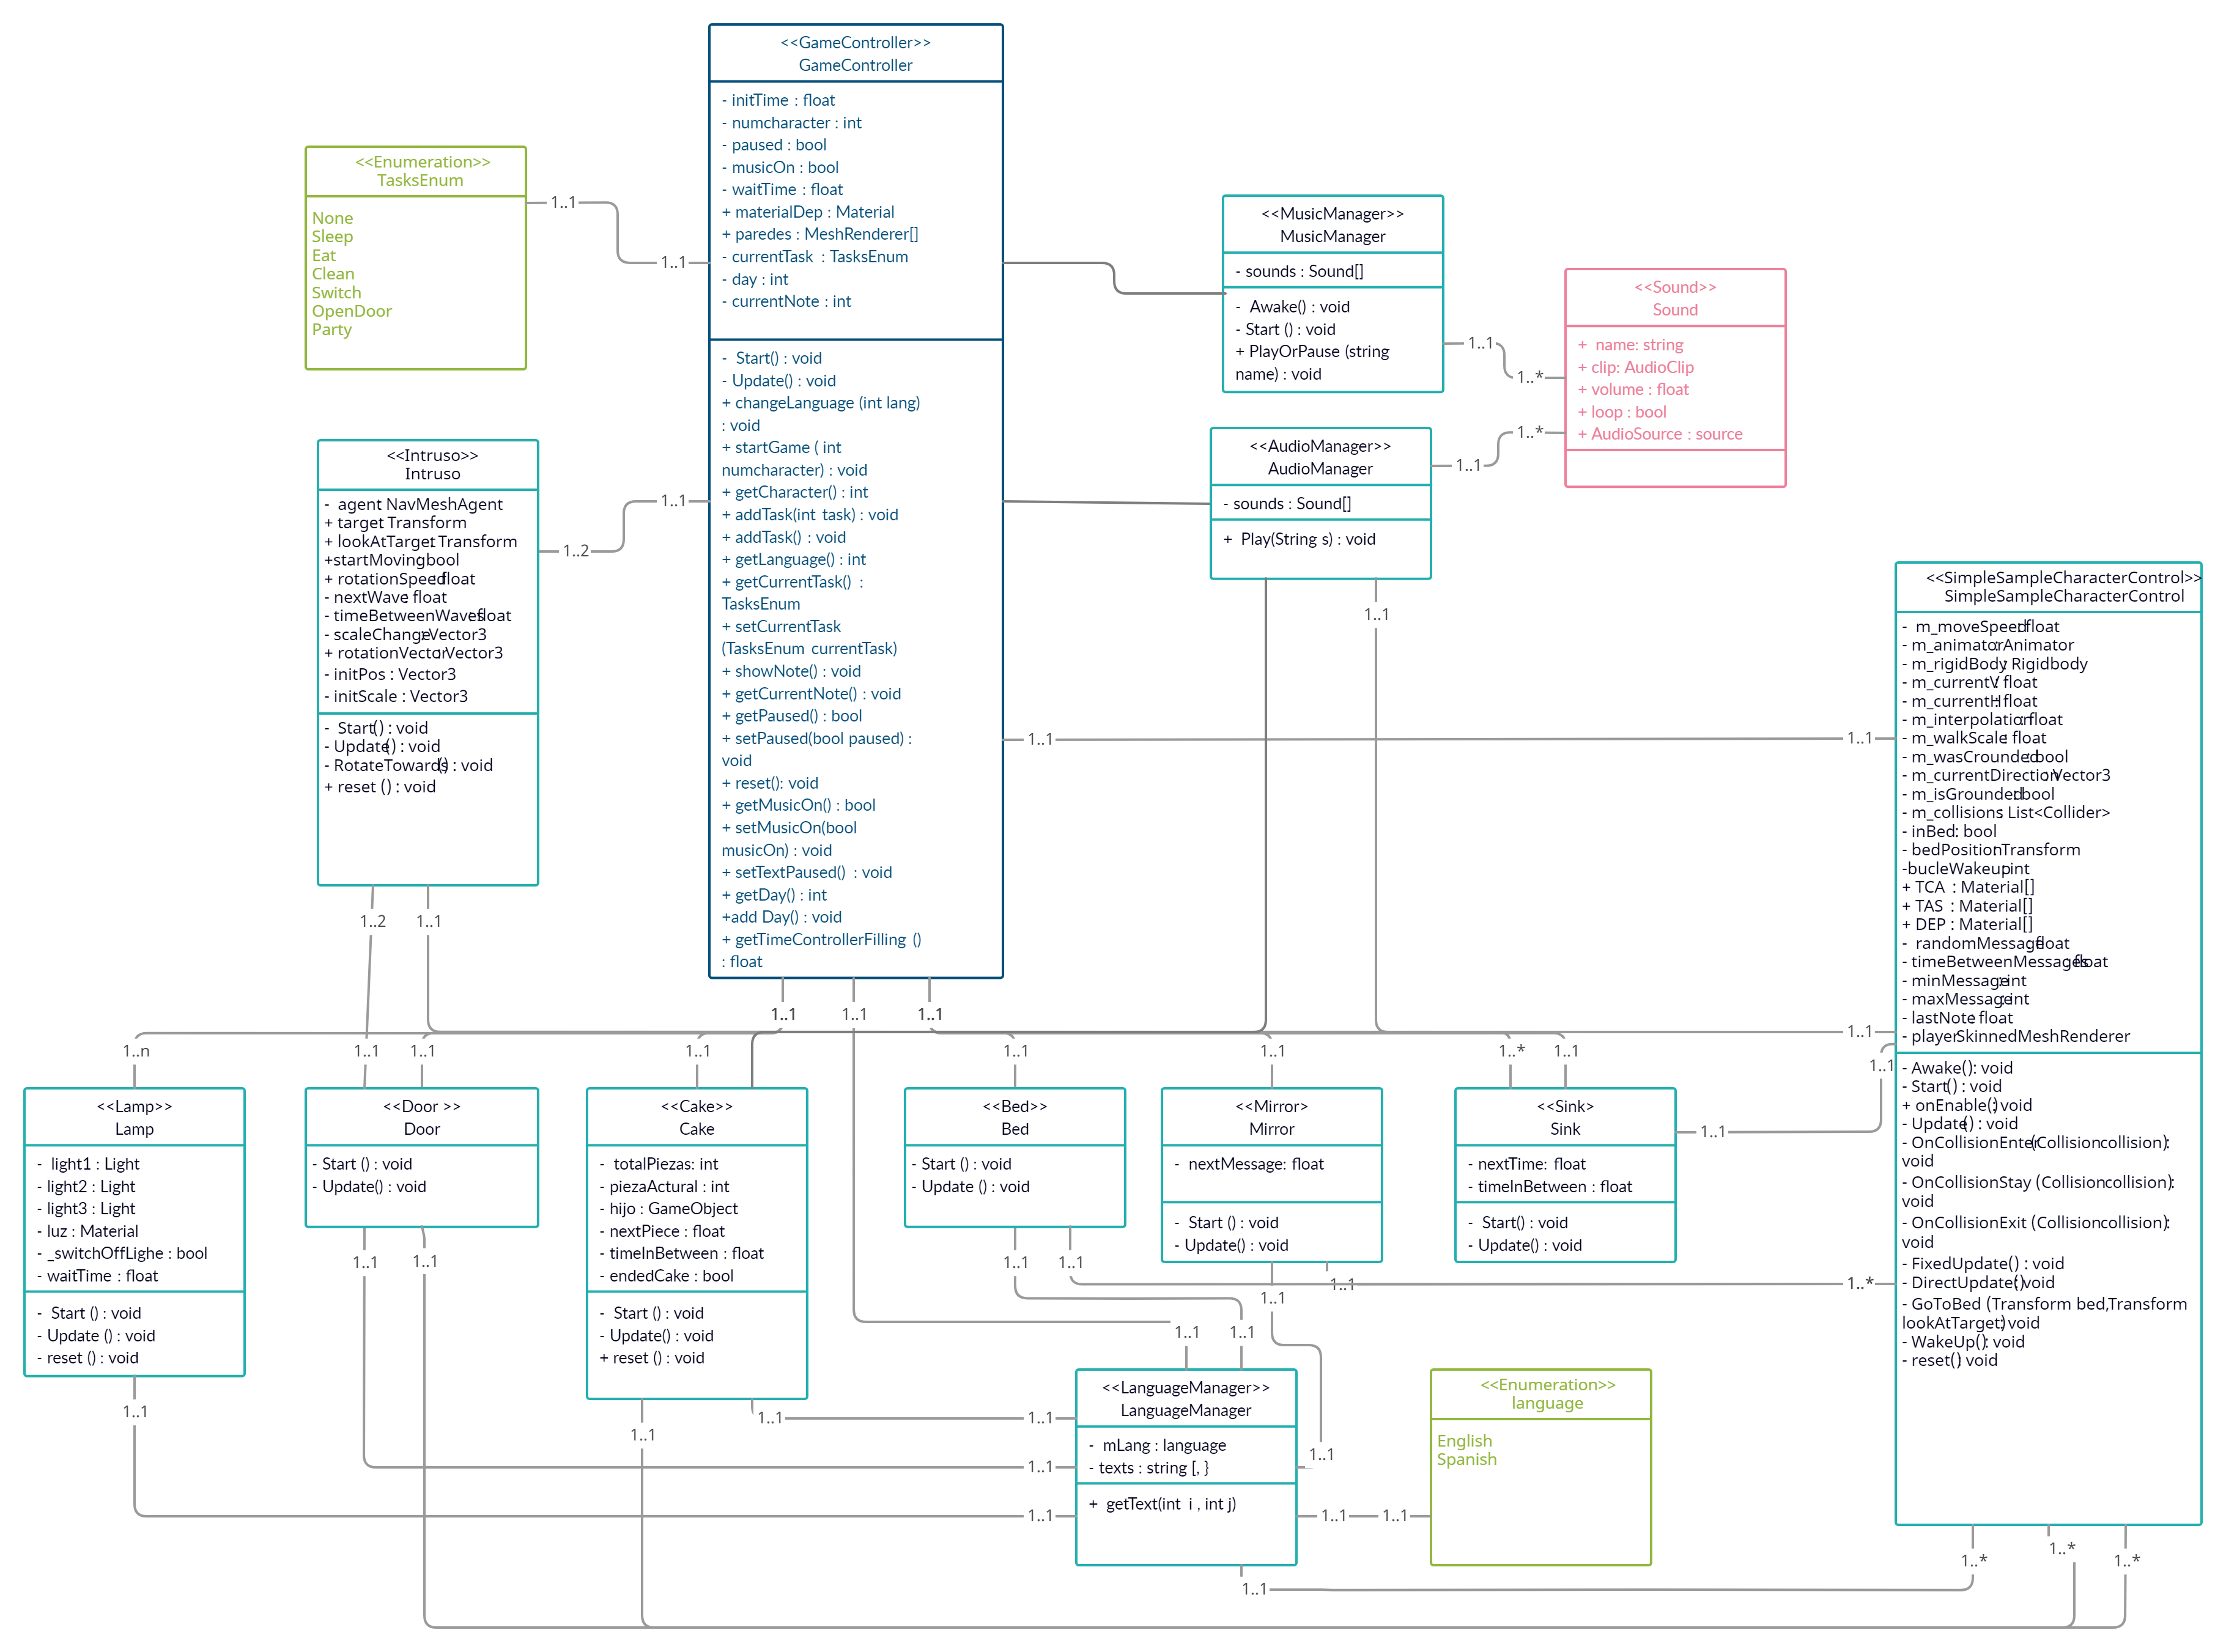
\includegraphics[width=1\linewidth]{TGF/Extra/UML.png}
    \caption{UML del prototipo}
    \label{fig:UML}
\end{figure}
\end{landscape}


\begin{figure}
	\centering
	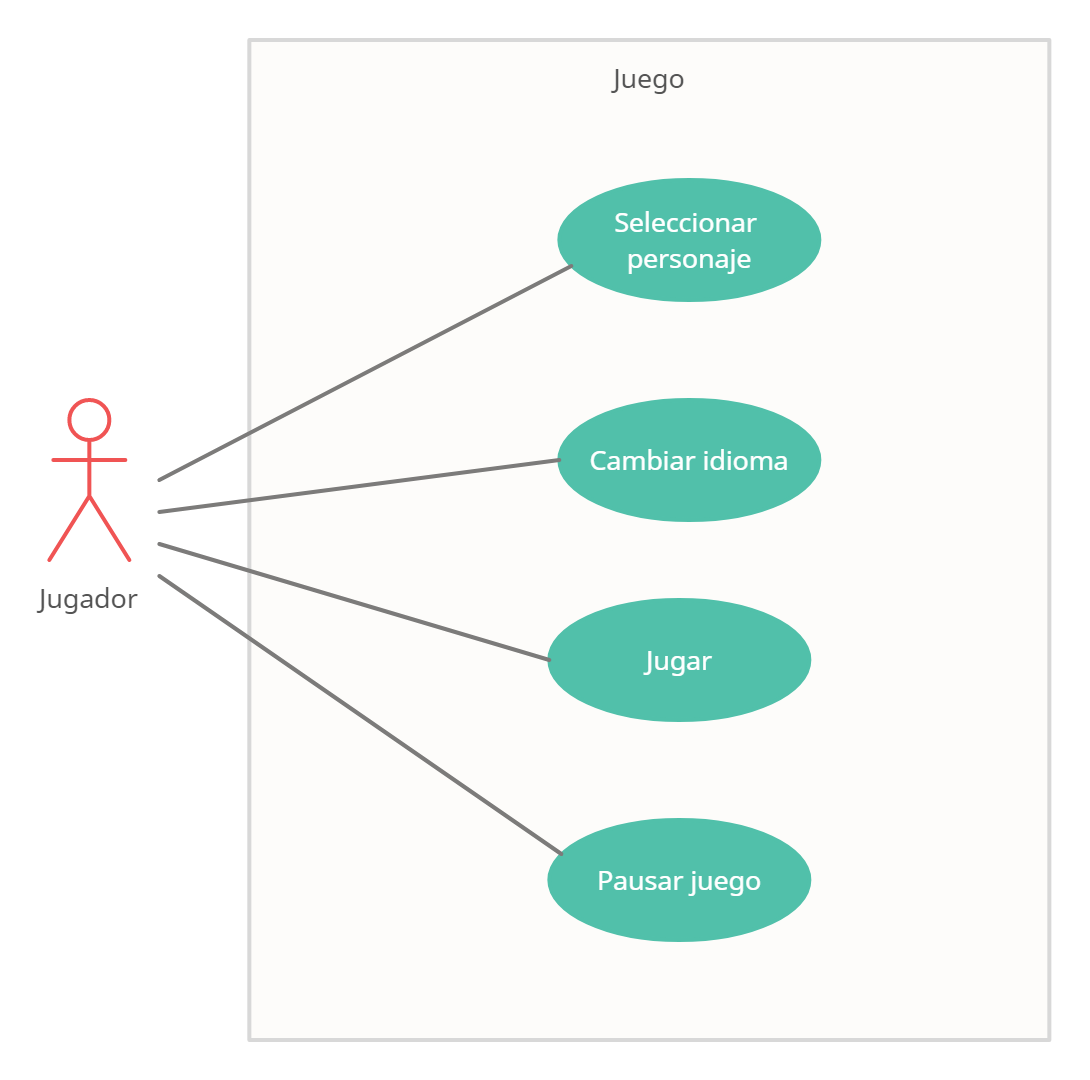
\includegraphics[width=.6\linewidth]{TGF/Extra/Casos de uso.png}
	\caption{Casos de uso}
	\label{fig:casosuso}
\end{figure}

\begin{landscape}
\begin{figure}
	\centering
	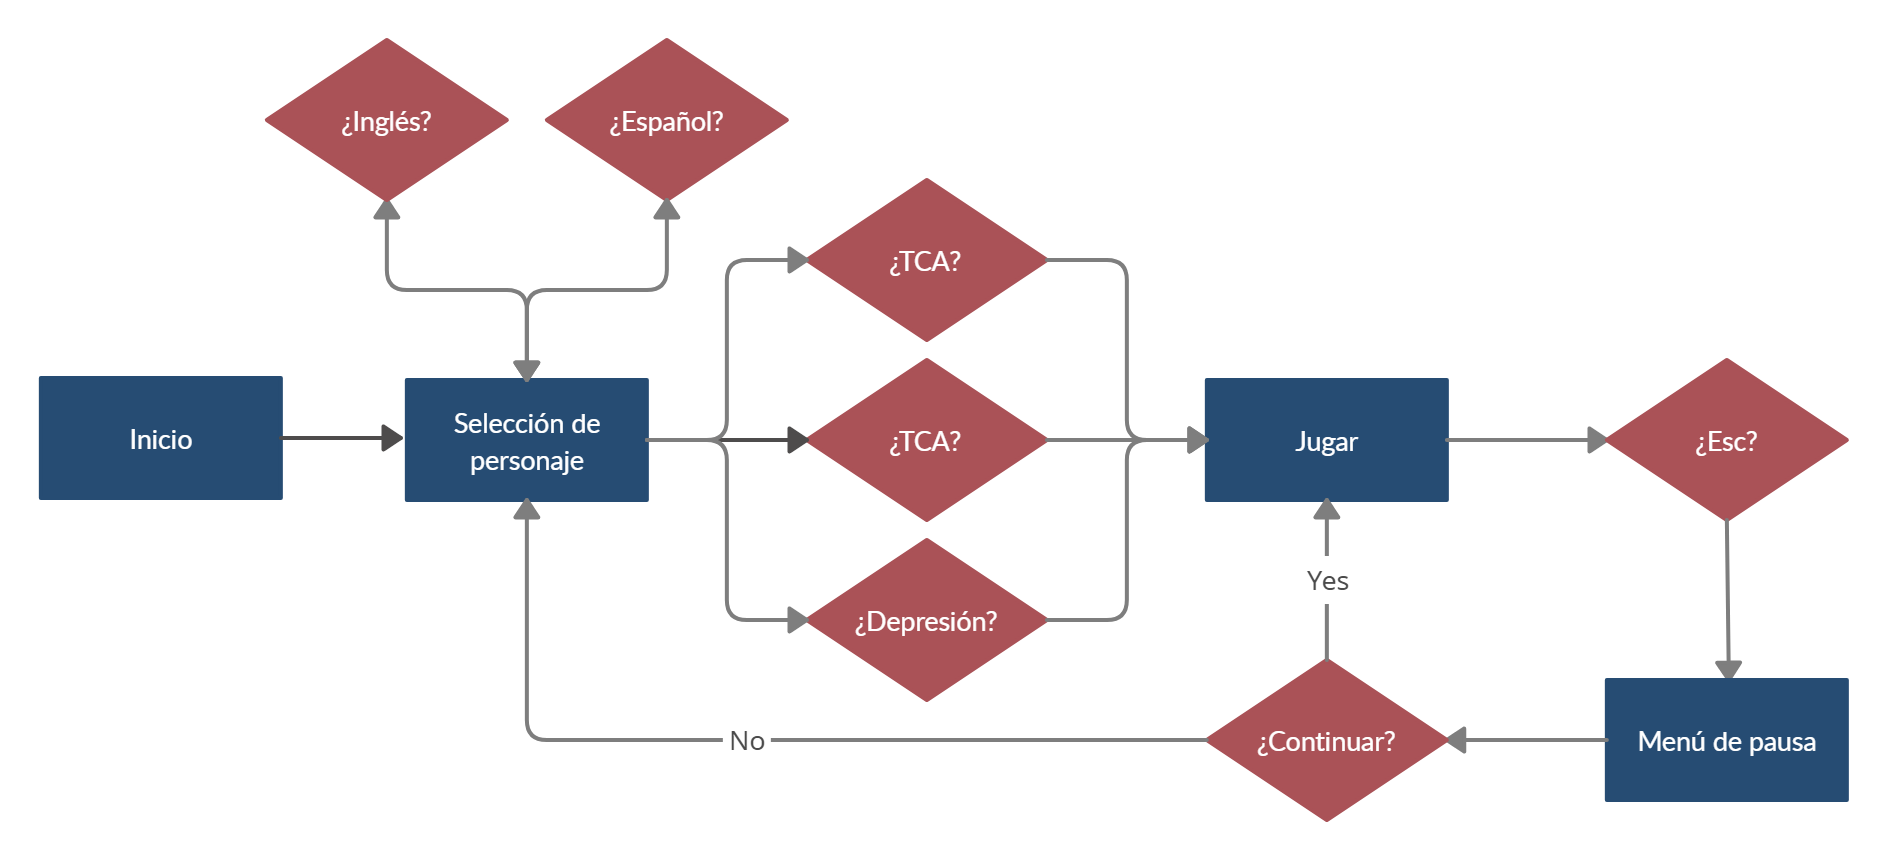
\includegraphics[width=.8\linewidth]{TGF/Extra/Flow.png}
	\caption{Diagrama de flujo}
	\label{fig:diagramaflujo}
\end{figure}
\end{landscape}


\subsection{Casos de uso}


El usuario podrá acceder a la selección de personajes, cambiar el idioma, jugar, y pausar el juego, como puede verse en la figura \ref{fig:casosuso}. 



\subsection{Diagrama de flujo}

El diagrama de flujo puede encontrarse en la figura \ref{fig:diagramaflujo}.





\section{Diseño de las artes}
\label{sec:diseñoArtes}
\subsection{Diseño gráfico y HUD}

\begin{figure}
	\centering
	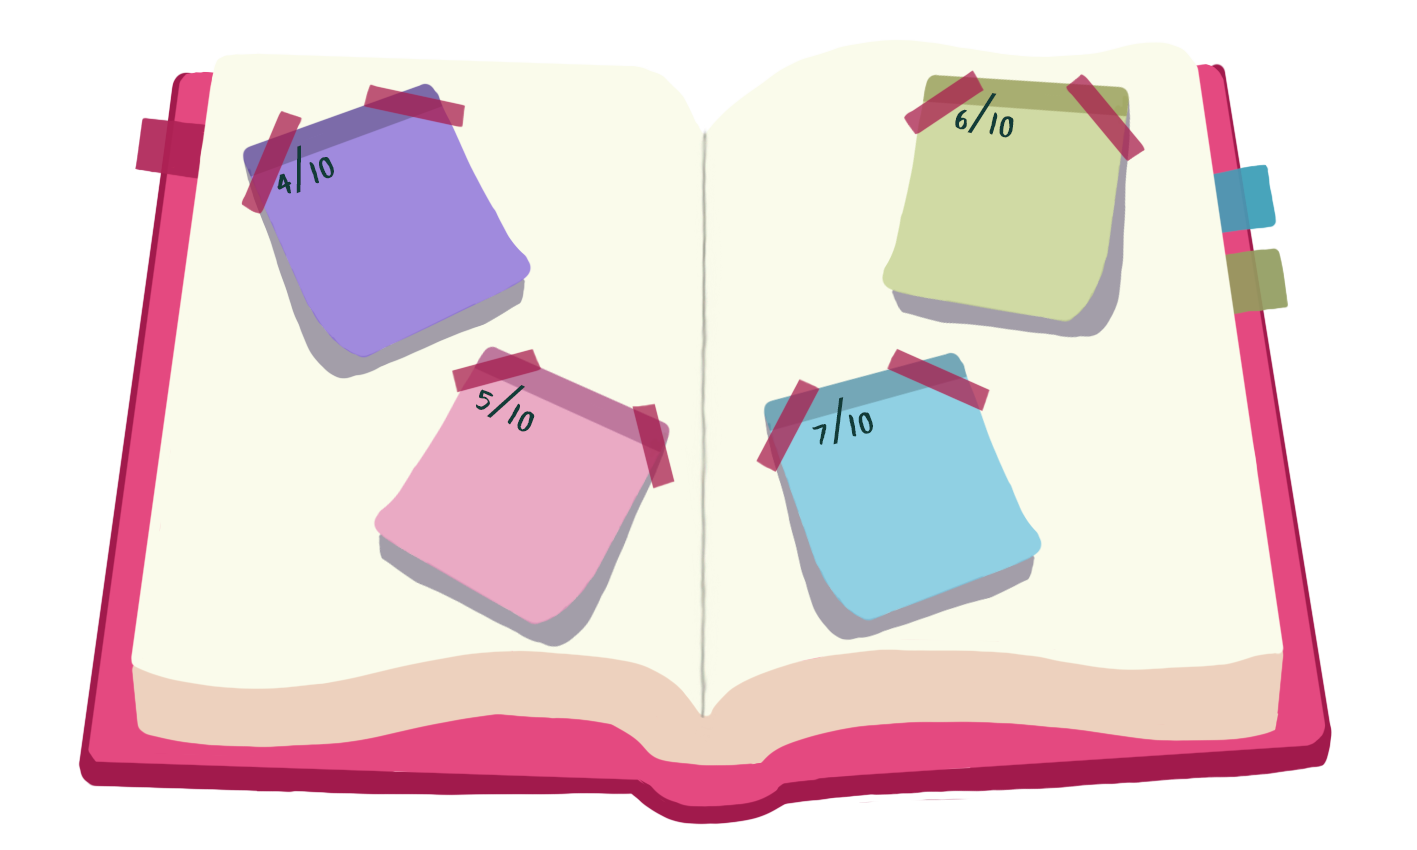
\includegraphics[width=.8\linewidth]{TGF/Artes/diarioNotas.png}
	\caption{Diario con todas las notas}
	\label{fig:diarioNotas}
\end{figure}

Para el diseño del juego se ha elegido una paleta de colores pastel, donde predomina el rosa claro. Esto es así por tratar un tema más ``suave'' o ``delicado''. La imagen principal se ha obtenido de \cite{imgInicio}. En cuanto al resto de elementos utilizados, se han creado con Photoshop, los botones, los iconos del diario, el diario abierto, las notas, etc. (Ver Figura \ref{fig:diarioNotas}). 

Como se puede ver en las figuras \ref{fig:UXInicio}, \ref{fig:UXSelec}, \ref{fig:UXPausa}, \ref{fig:UXHUD} y \ref{fig:UXHUD2}, se ha intentado tener un diseño sencillo y claro, que no enturbie demasiado la pantalla de juego y que proporcione la información necesaria en cada momento. Además, se ofrecen botones para poder cambiar el idioma, haciendo el juego más accesible, también para poder encender o apagar la música, para garantizar un mayor control por parte del jugador, y para salir del juego en cualquier momento o reanudarlo, gracias al menú de pausa. 



\begin{figure}
	\centering
	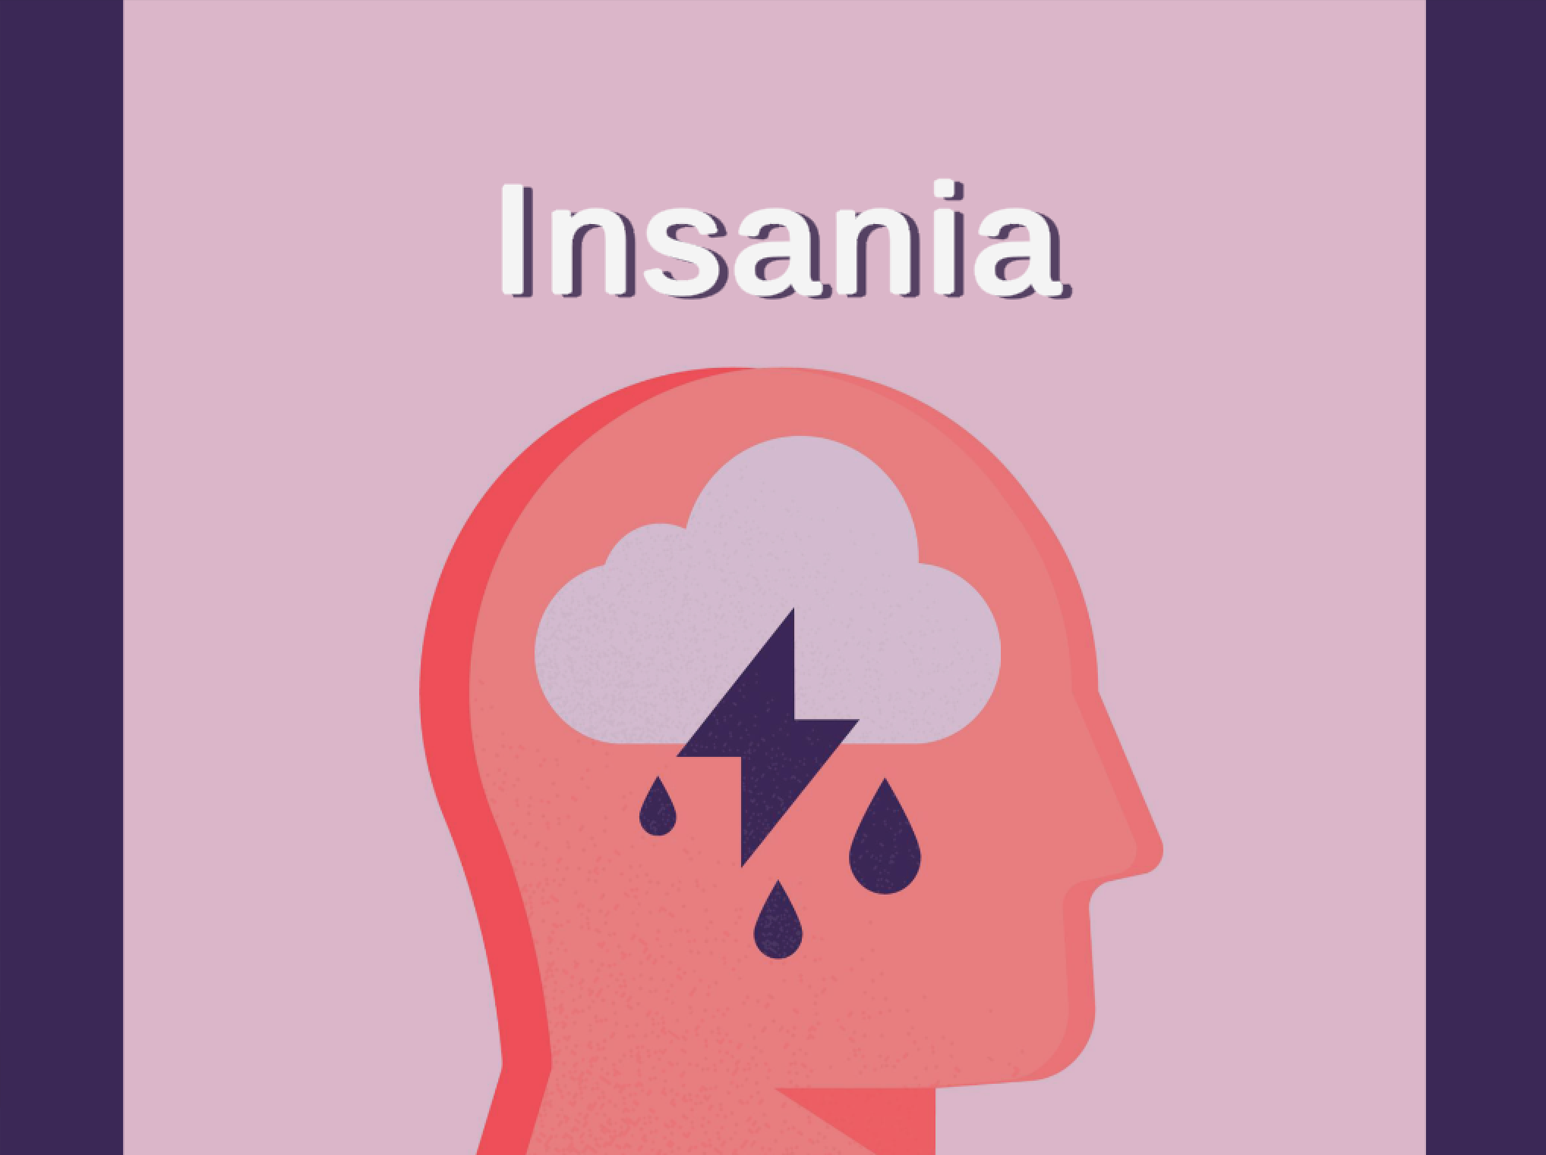
\includegraphics[width=.8\linewidth]{TGF/Artes/Portada.png}
	\caption{Pantalla de Inicio}
	\label{fig:UXInicio}
\end{figure}

\begin{figure}
	\centering
	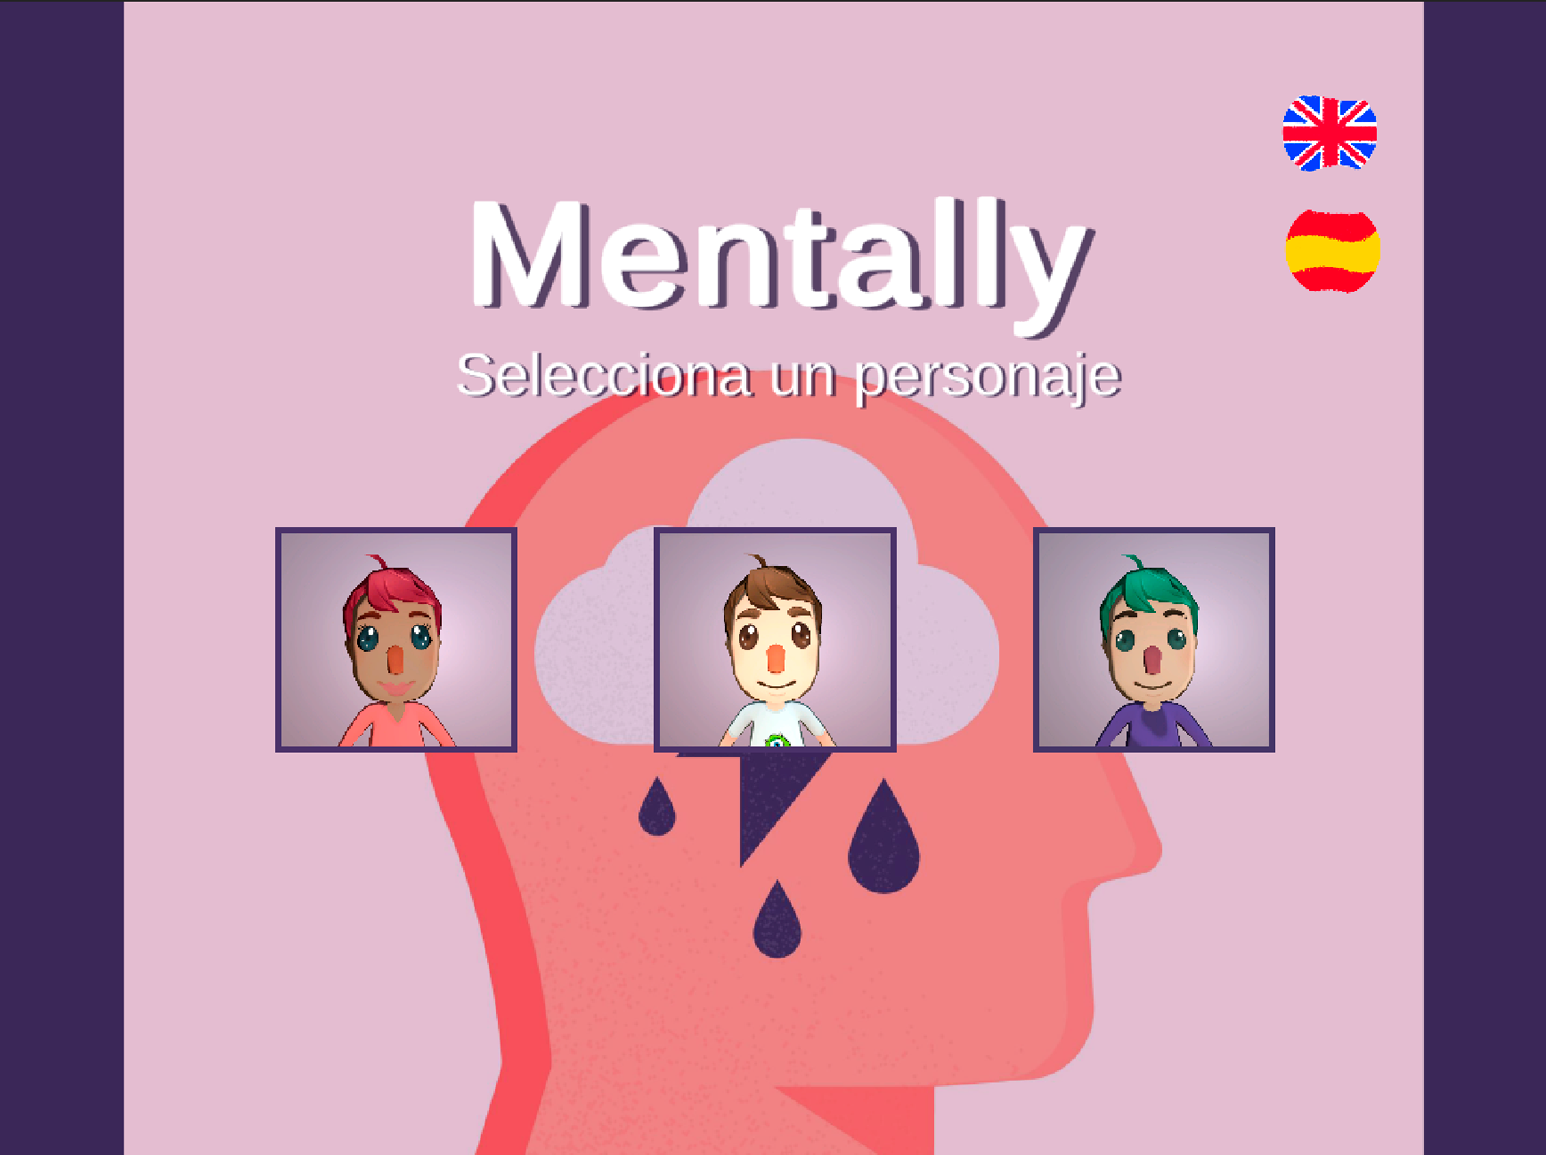
\includegraphics[width=.8\linewidth]{TGF/Artes/Personajes.png}
	\caption{Pantalla de selección de personaje}
	\label{fig:UXSelec}
\end{figure}

\begin{figure}
	\centering
	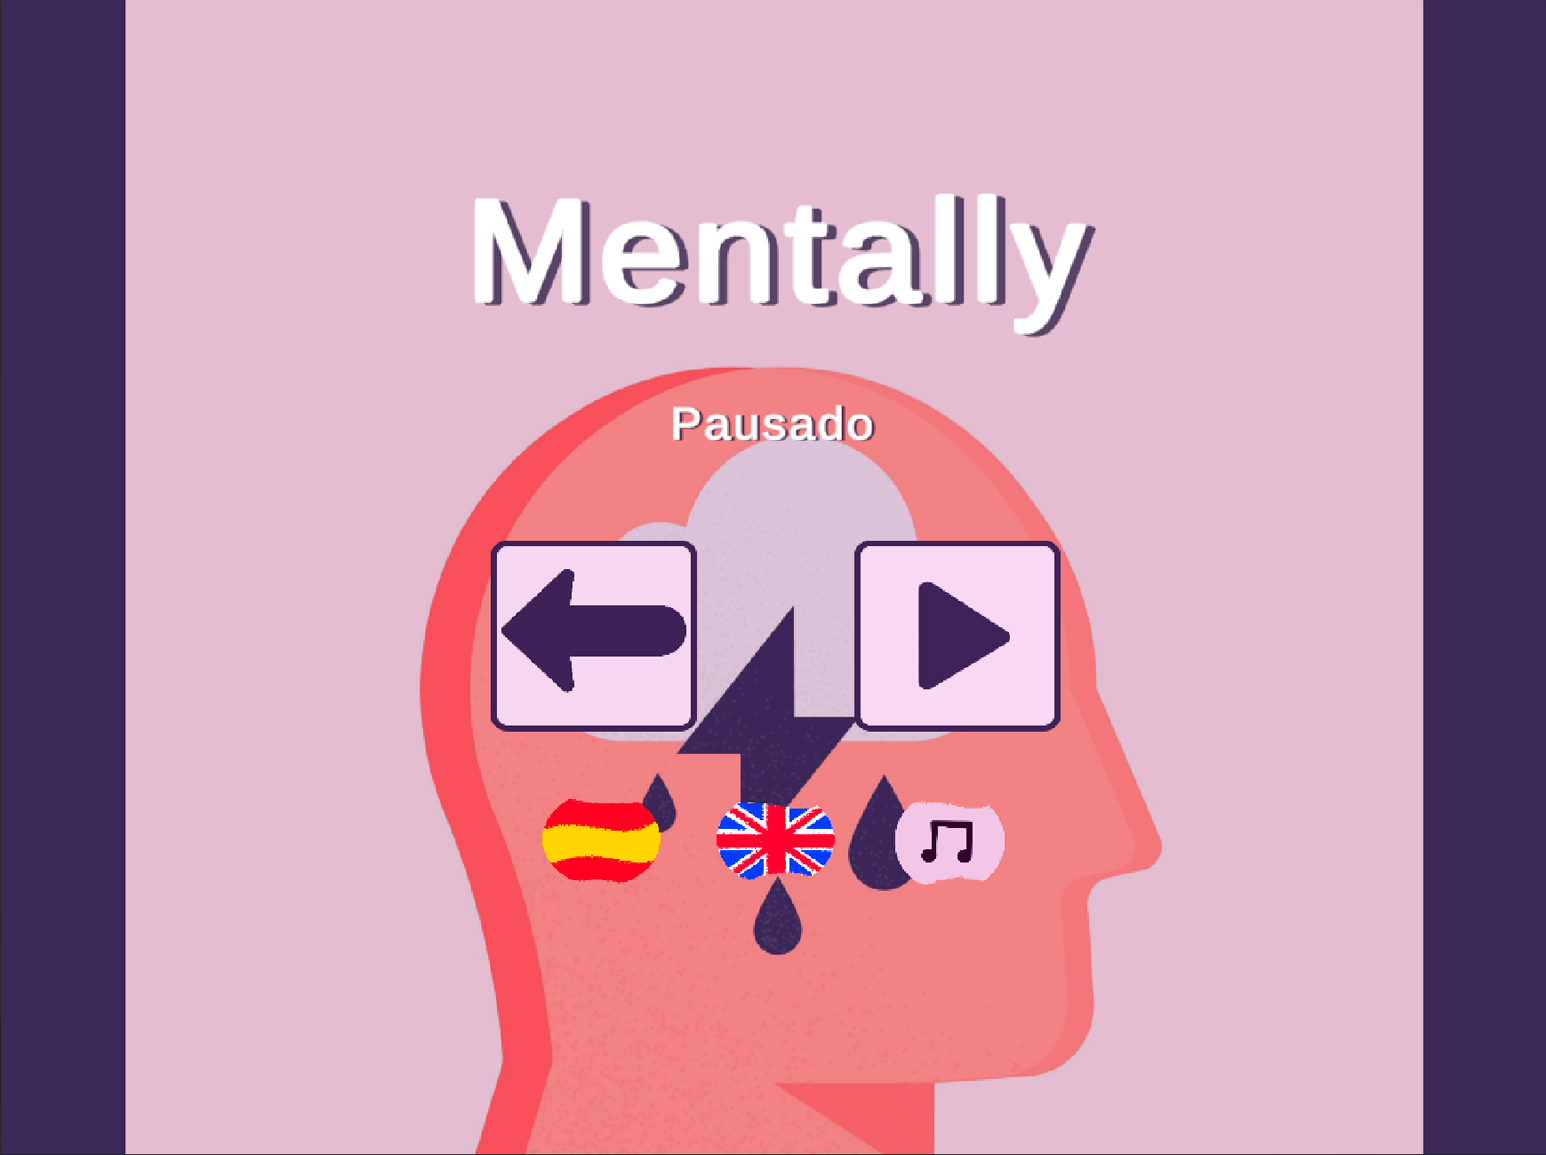
\includegraphics[width=.8\linewidth]{TGF/Artes/Pausa.png}
	\caption{Pantalla de menú de pausa}
	\label{fig:UXPausa}
\end{figure}

\begin{figure}
	\centering
	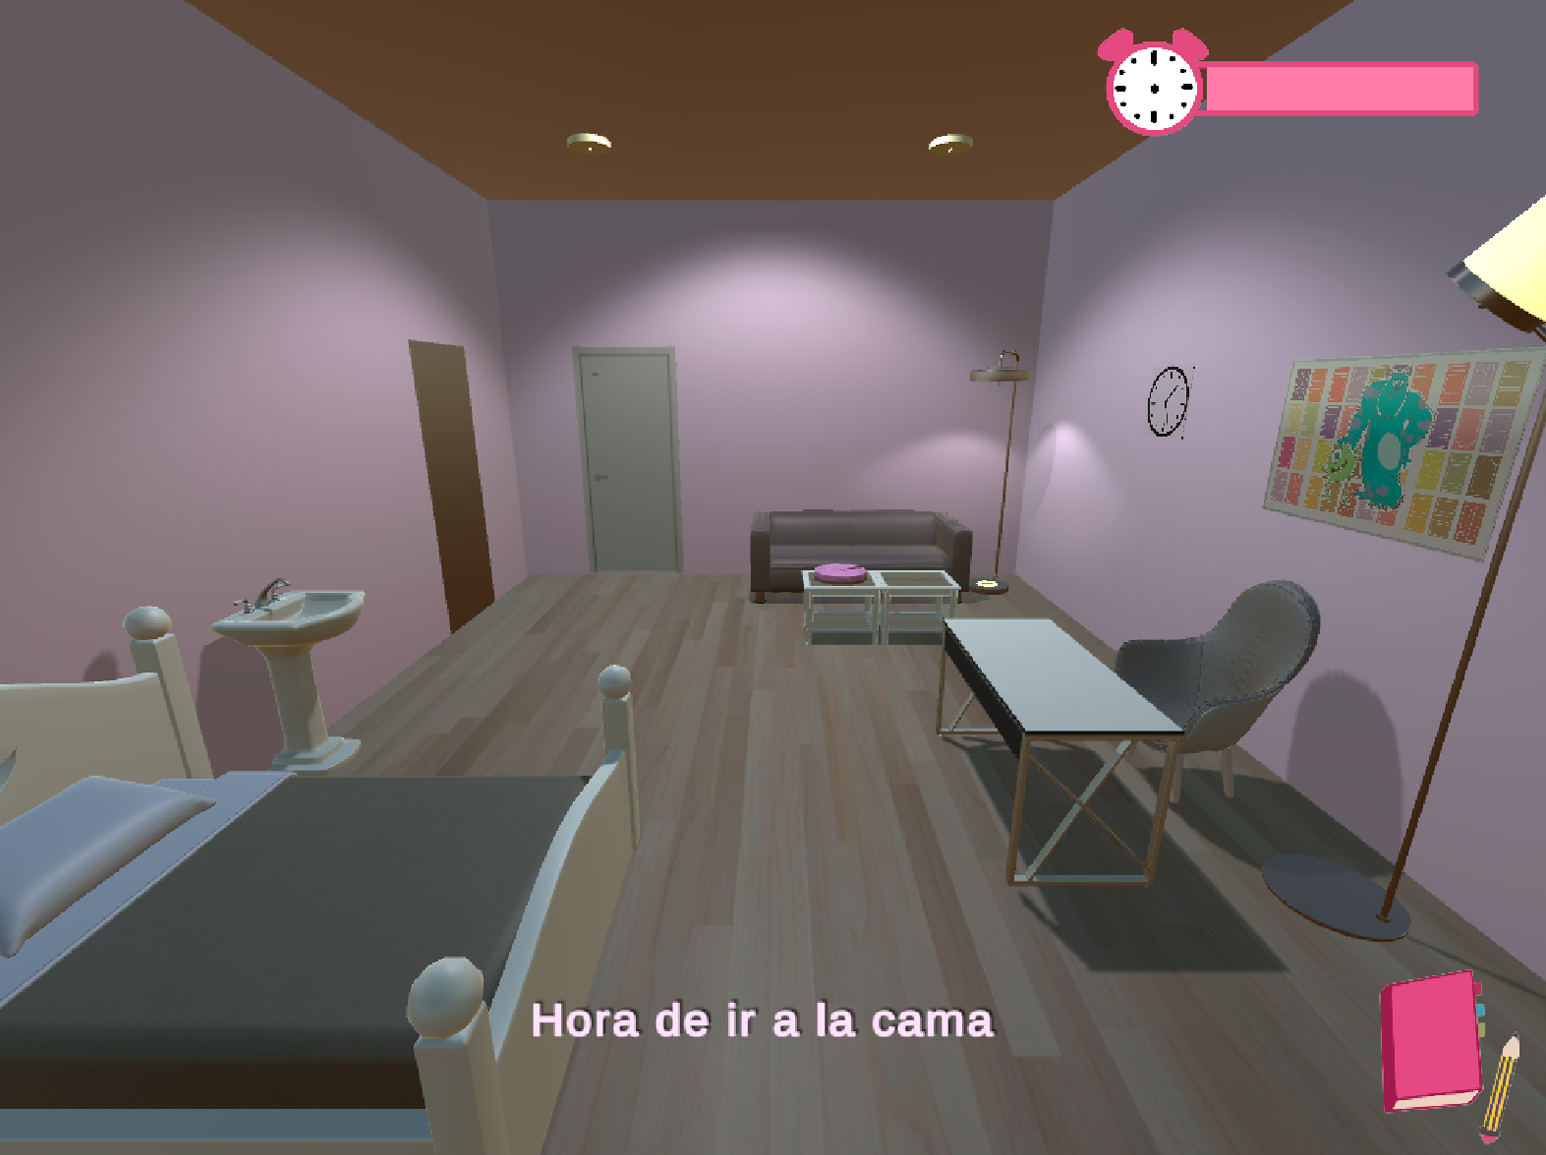
\includegraphics[width=.8\linewidth]{TGF/Artes/UX basic.png}
	\caption{HUD del juego}
	\label{fig:UXHUD}
\end{figure}

\begin{figure}
	\centering
	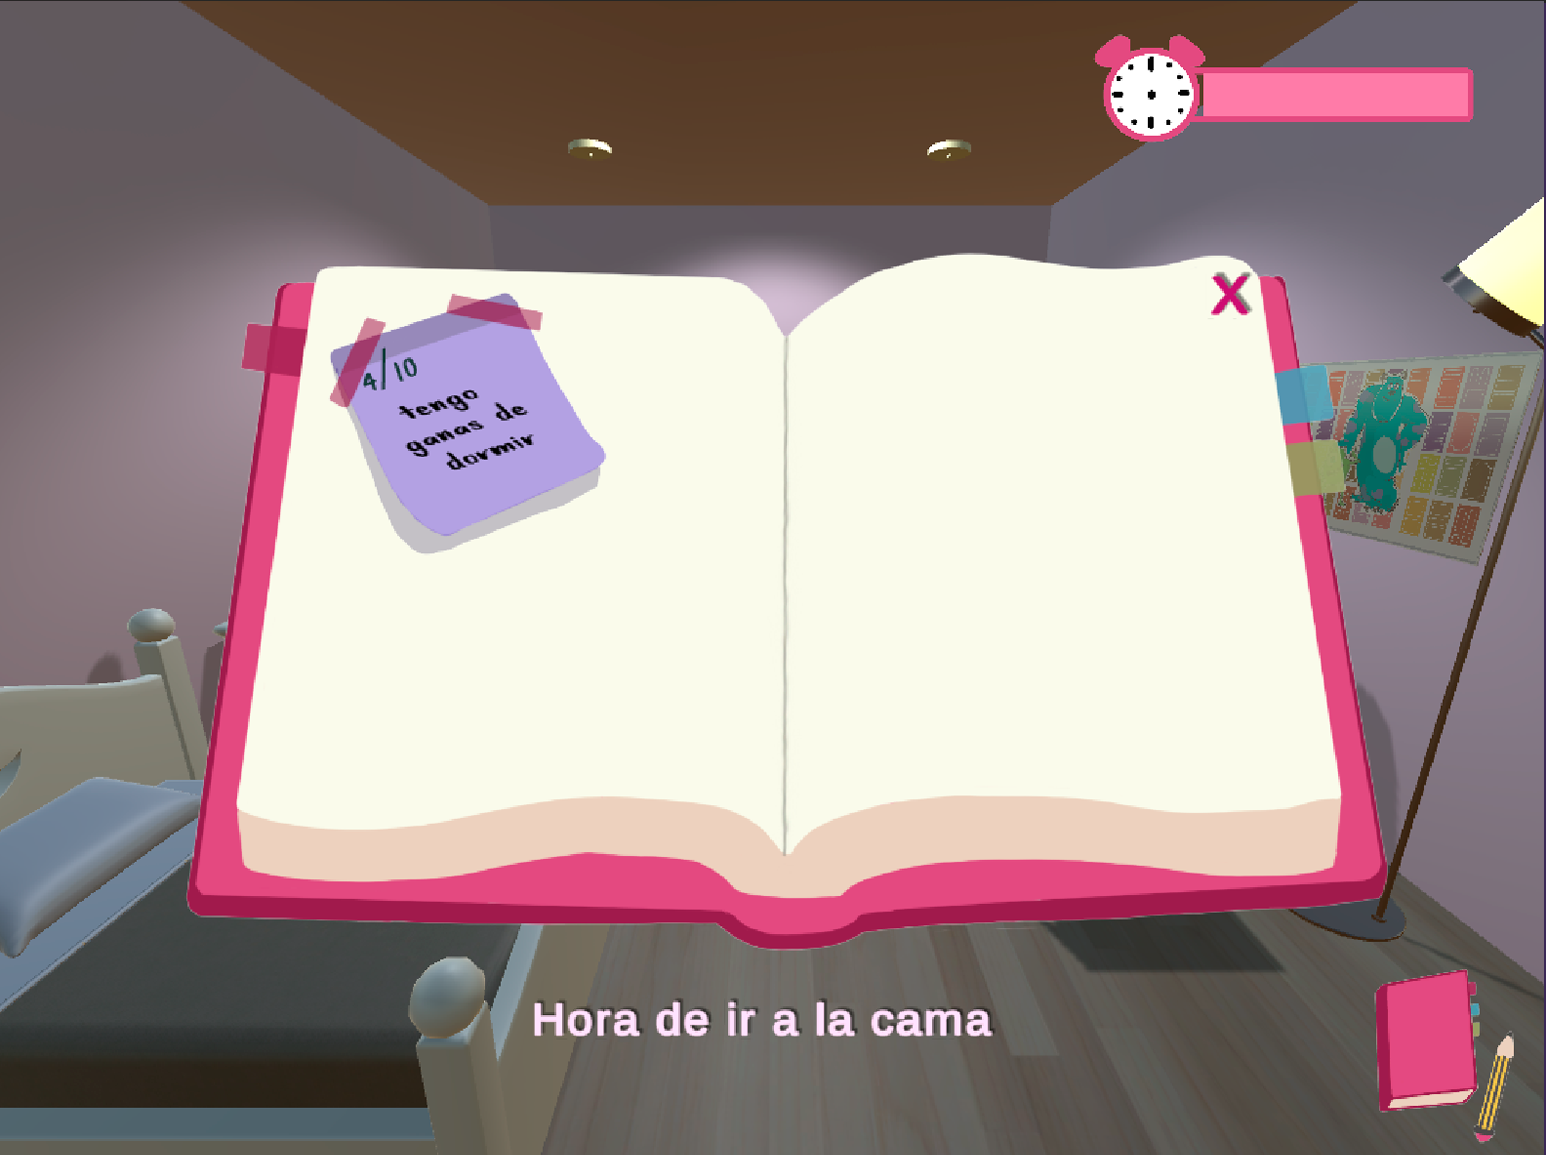
\includegraphics[width=.8\linewidth]{TGF/Artes/UX diario abierto.png}
	\caption{HUD del juego con el diario abierto}
	\label{fig:UXHUD2}
\end{figure}




Pantalla de inicio (Ver Figura \ref{fig:UXInicio})

Selección de personaje (Ver Figura \ref{fig:UXSelec})

Menú de pausa (Ver Figura \ref{fig:UXPausa})

HUD del juego (Ver Figura \ref{fig:UXHUD})

HUD del juego con diario abierto (Ver Figura \ref{fig:UXHUD2})





\subsection{Escenario y personajes}
\subsubsection{Escenario}


\begin{figure}
	\centering
	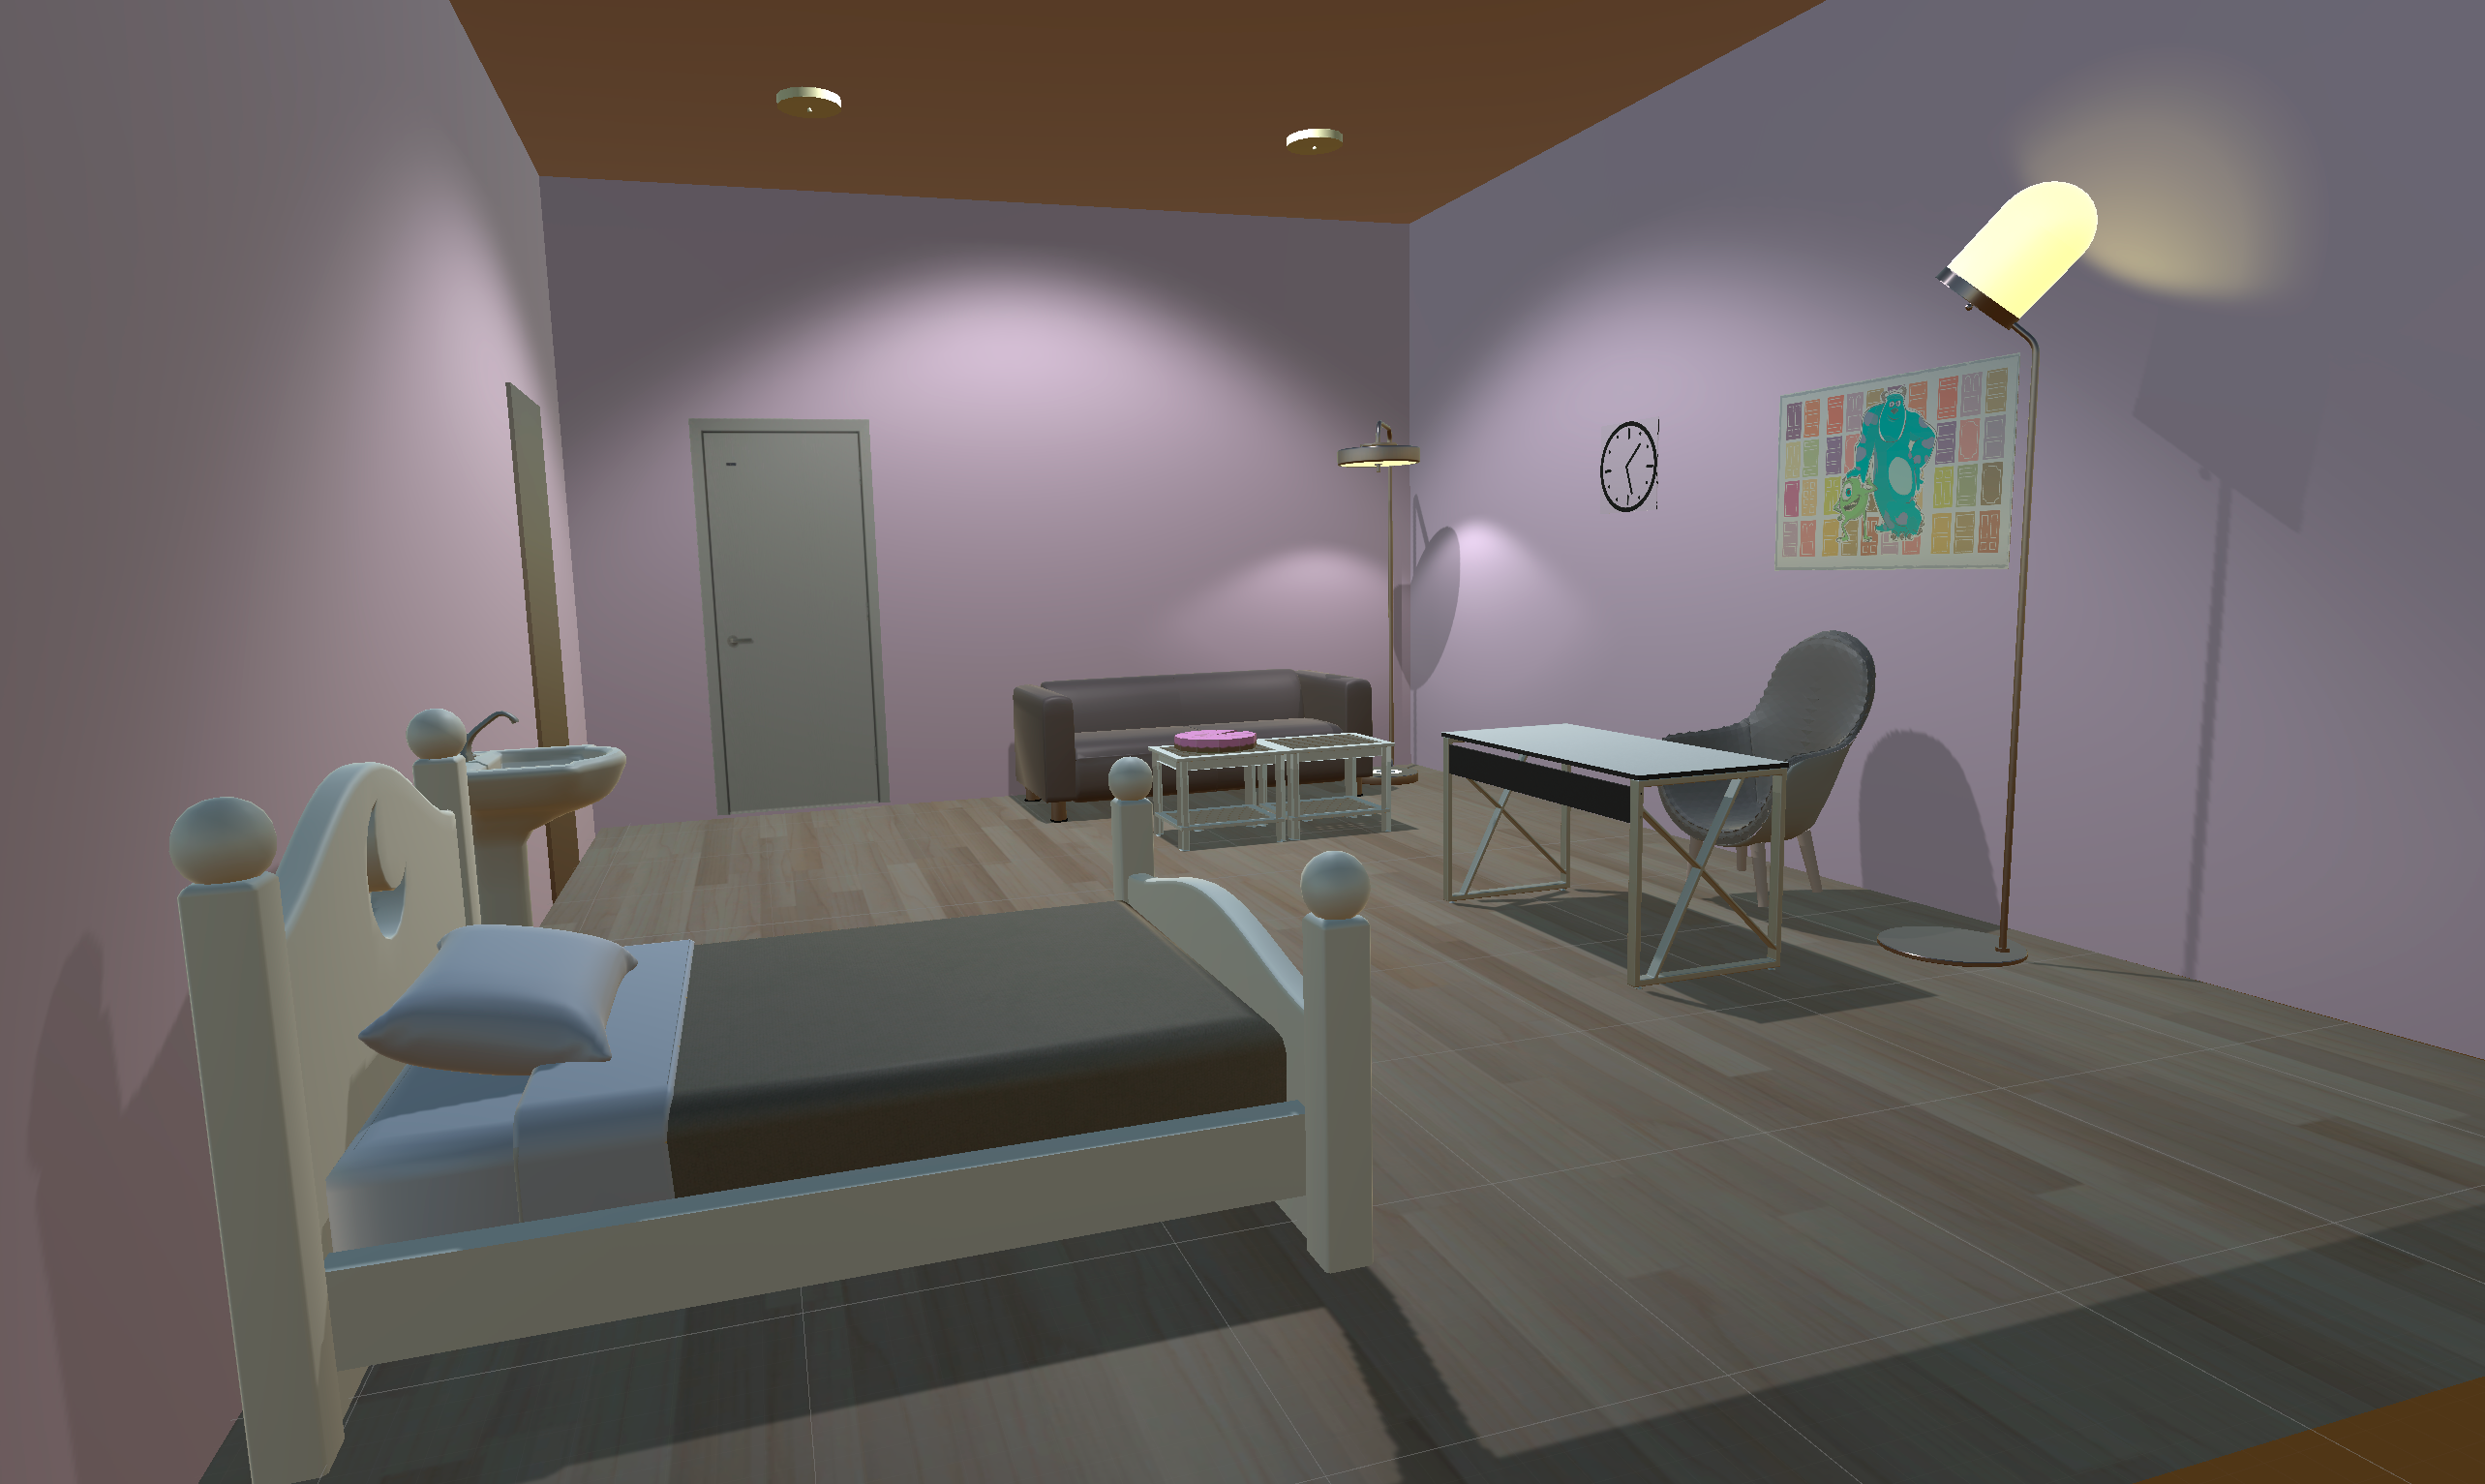
\includegraphics[width=1\linewidth]{TGF/Artes/Escenario.png}
	\caption{Escenario completo}
	\label{fig:ArtesEsce}
\end{figure}

\begin{figure}
	\centering
	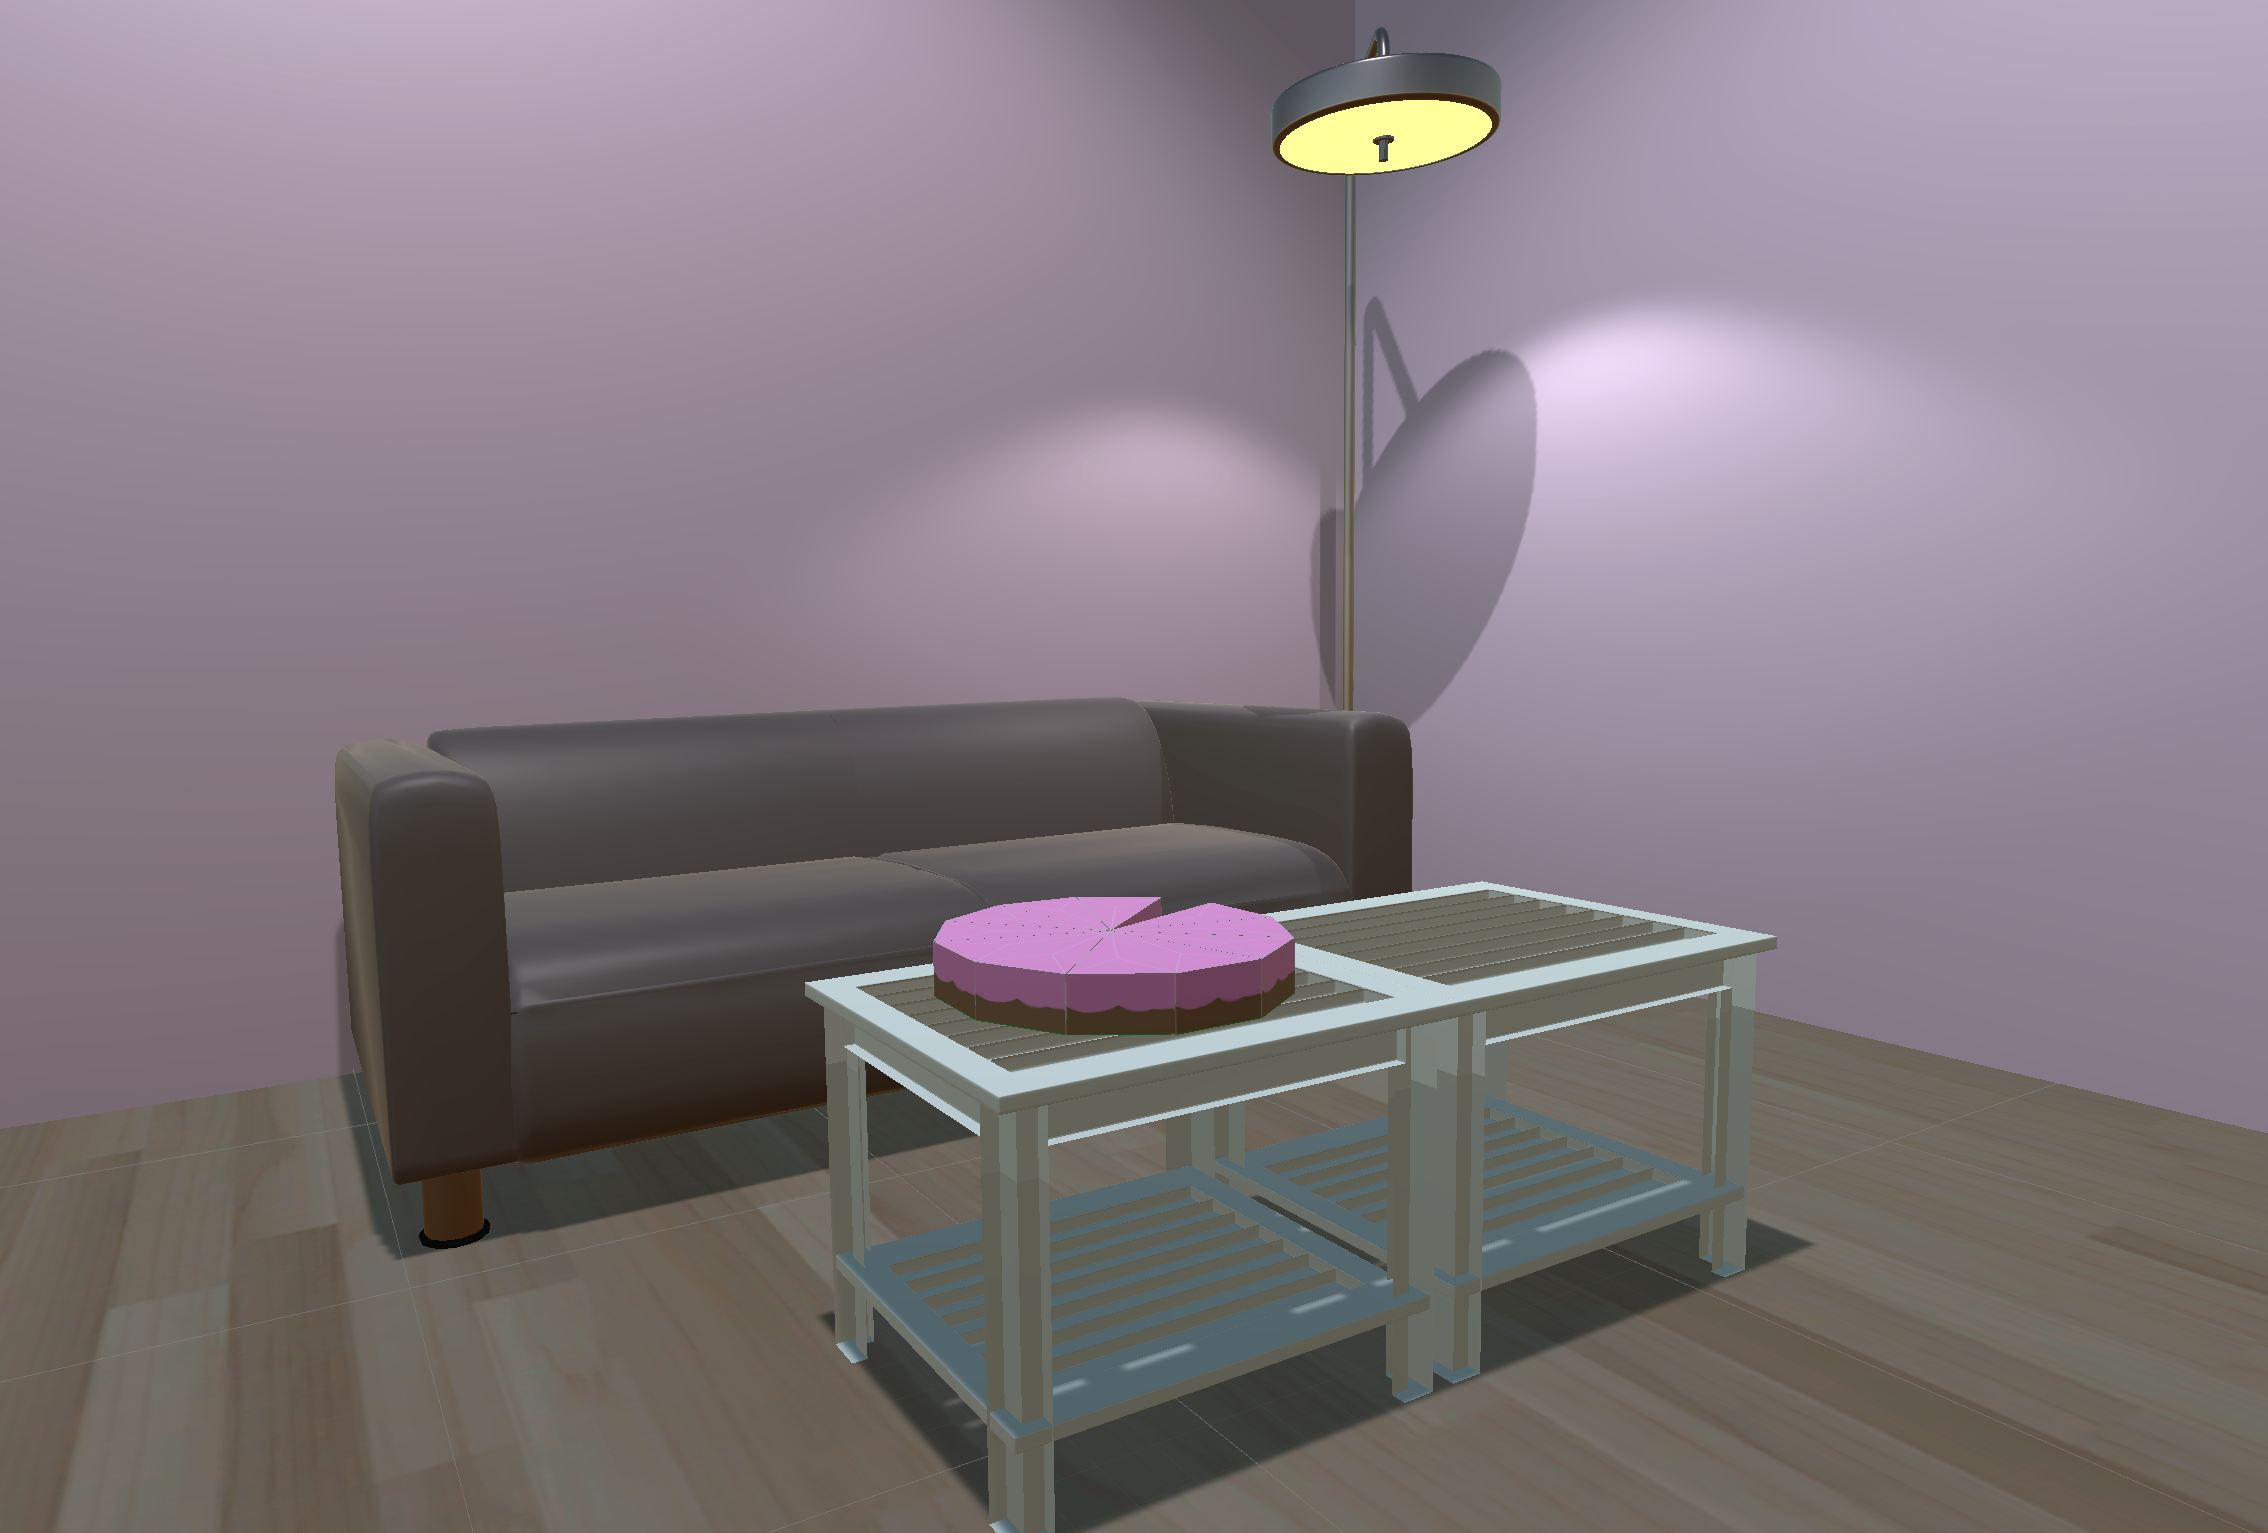
\includegraphics[width=.9\linewidth]{TGF/Artes/Saloncito.png}
	\caption{Salón}
	\label{fig:ArtesSalon}
\end{figure}

\begin{figure}
	\centering
	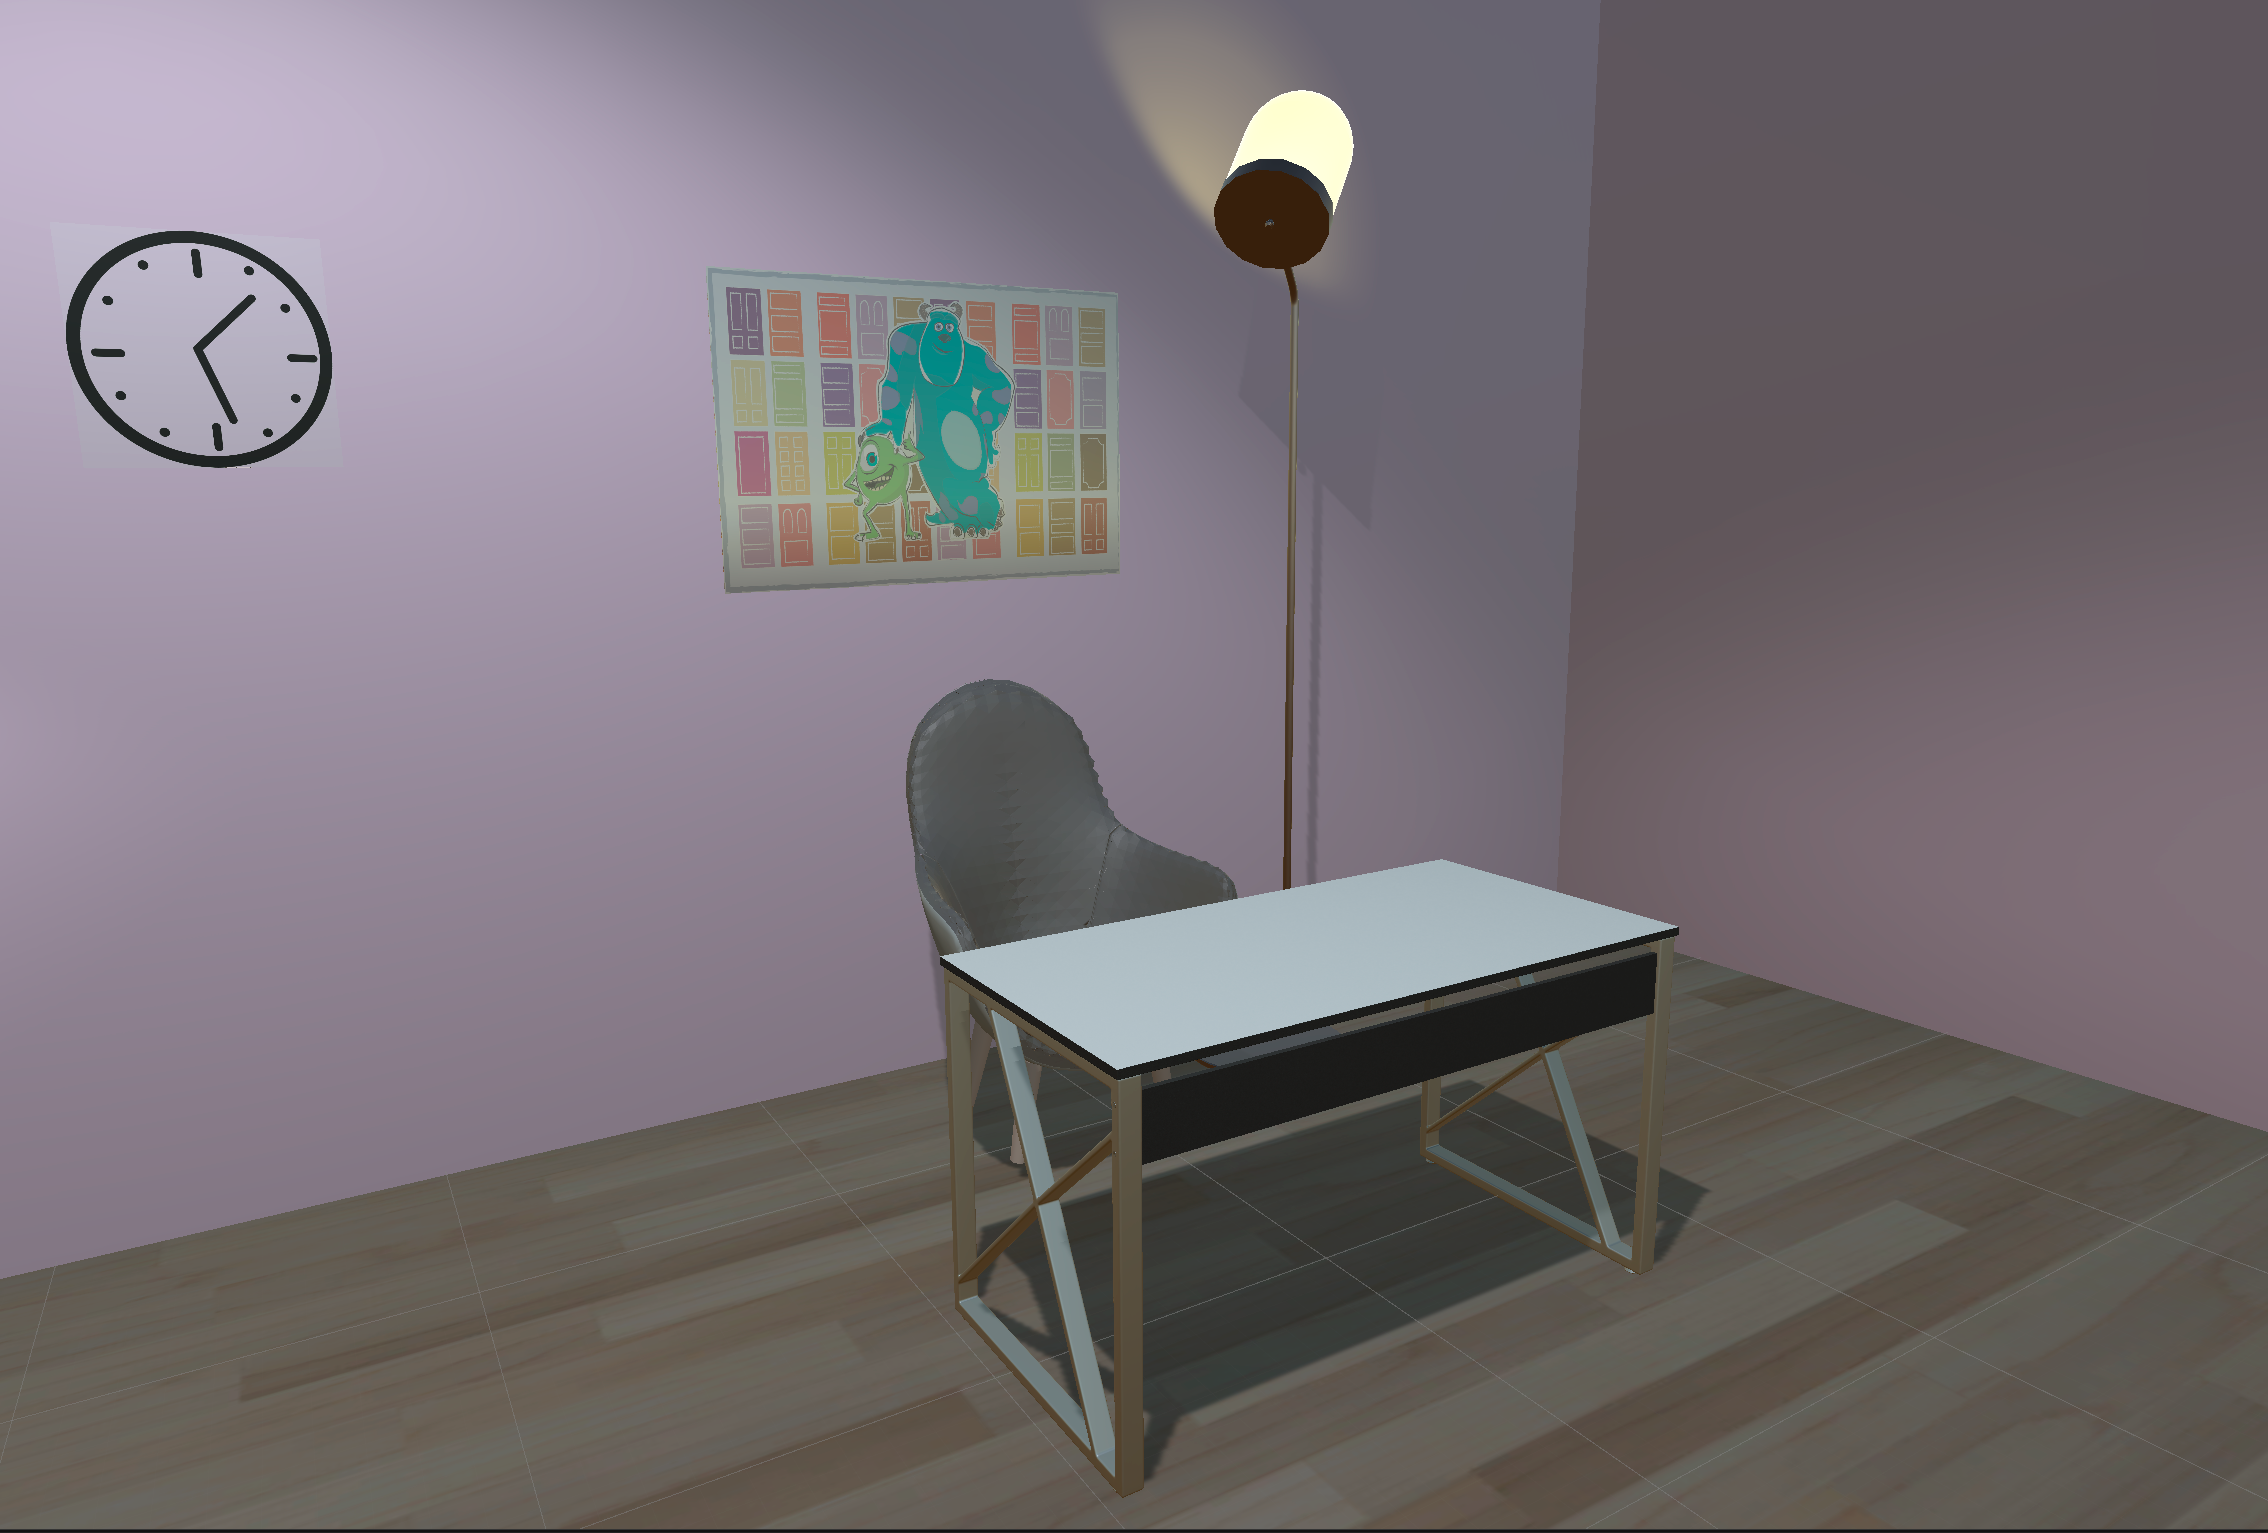
\includegraphics[width=.9\linewidth]{TGF/Artes/Despachito.png}
	\caption{Despacho}
	\label{fig:ArtesDesp}
\end{figure}

\begin{figure}
	\centering
	\includegraphics[width=.9\linewidth]{TGF/Artes/Habitación.png}
	\caption{Habitación}
	\label{fig:ArtesHab}
\end{figure}


Visión completa del escenario (Ver figura \ref{fig:ArtesEsce})

Salón (Ver figura \ref{fig:ArtesSalon})

Despacho (Ver figura \ref{fig:ArtesDesp})

Habitación (Ver figura \ref{fig:ArtesHab})

Algunos de los modelos han sido obtenidos de \cite{refBedBath}, en el caso de los muebles de la habitación y baño, \cite{refDesk}, en el caso del escritorio del despacho o \cite{refSofa}, en el caso del sofá. Otros modelos, como la tarta, han sido realizados en 3dsMax. 

\begin{figure}
	\centering
	\begin{subfigure}{.5\textwidth}
		\centering
		
\includegraphics[width=.95\linewidth]{TGF/Artes/TexBed.png}
		\caption{Mapa de UVs de la cama antiguo}
	\end{subfigure}%
	\begin{subfigure}{.5\textwidth}
		\centering
		
\includegraphics[width=.95\linewidth]{TGF/Artes/TexBed2.png}
		\caption{Mapa de UVs de la cama nuevo}
	\end{subfigure}
	\caption{Mapas de UVs de la cama}
	\label{fig:texBed}
\end{figure}


\begin{figure}
	\centering
	\begin{subfigure}{.5\textwidth}
		\centering
		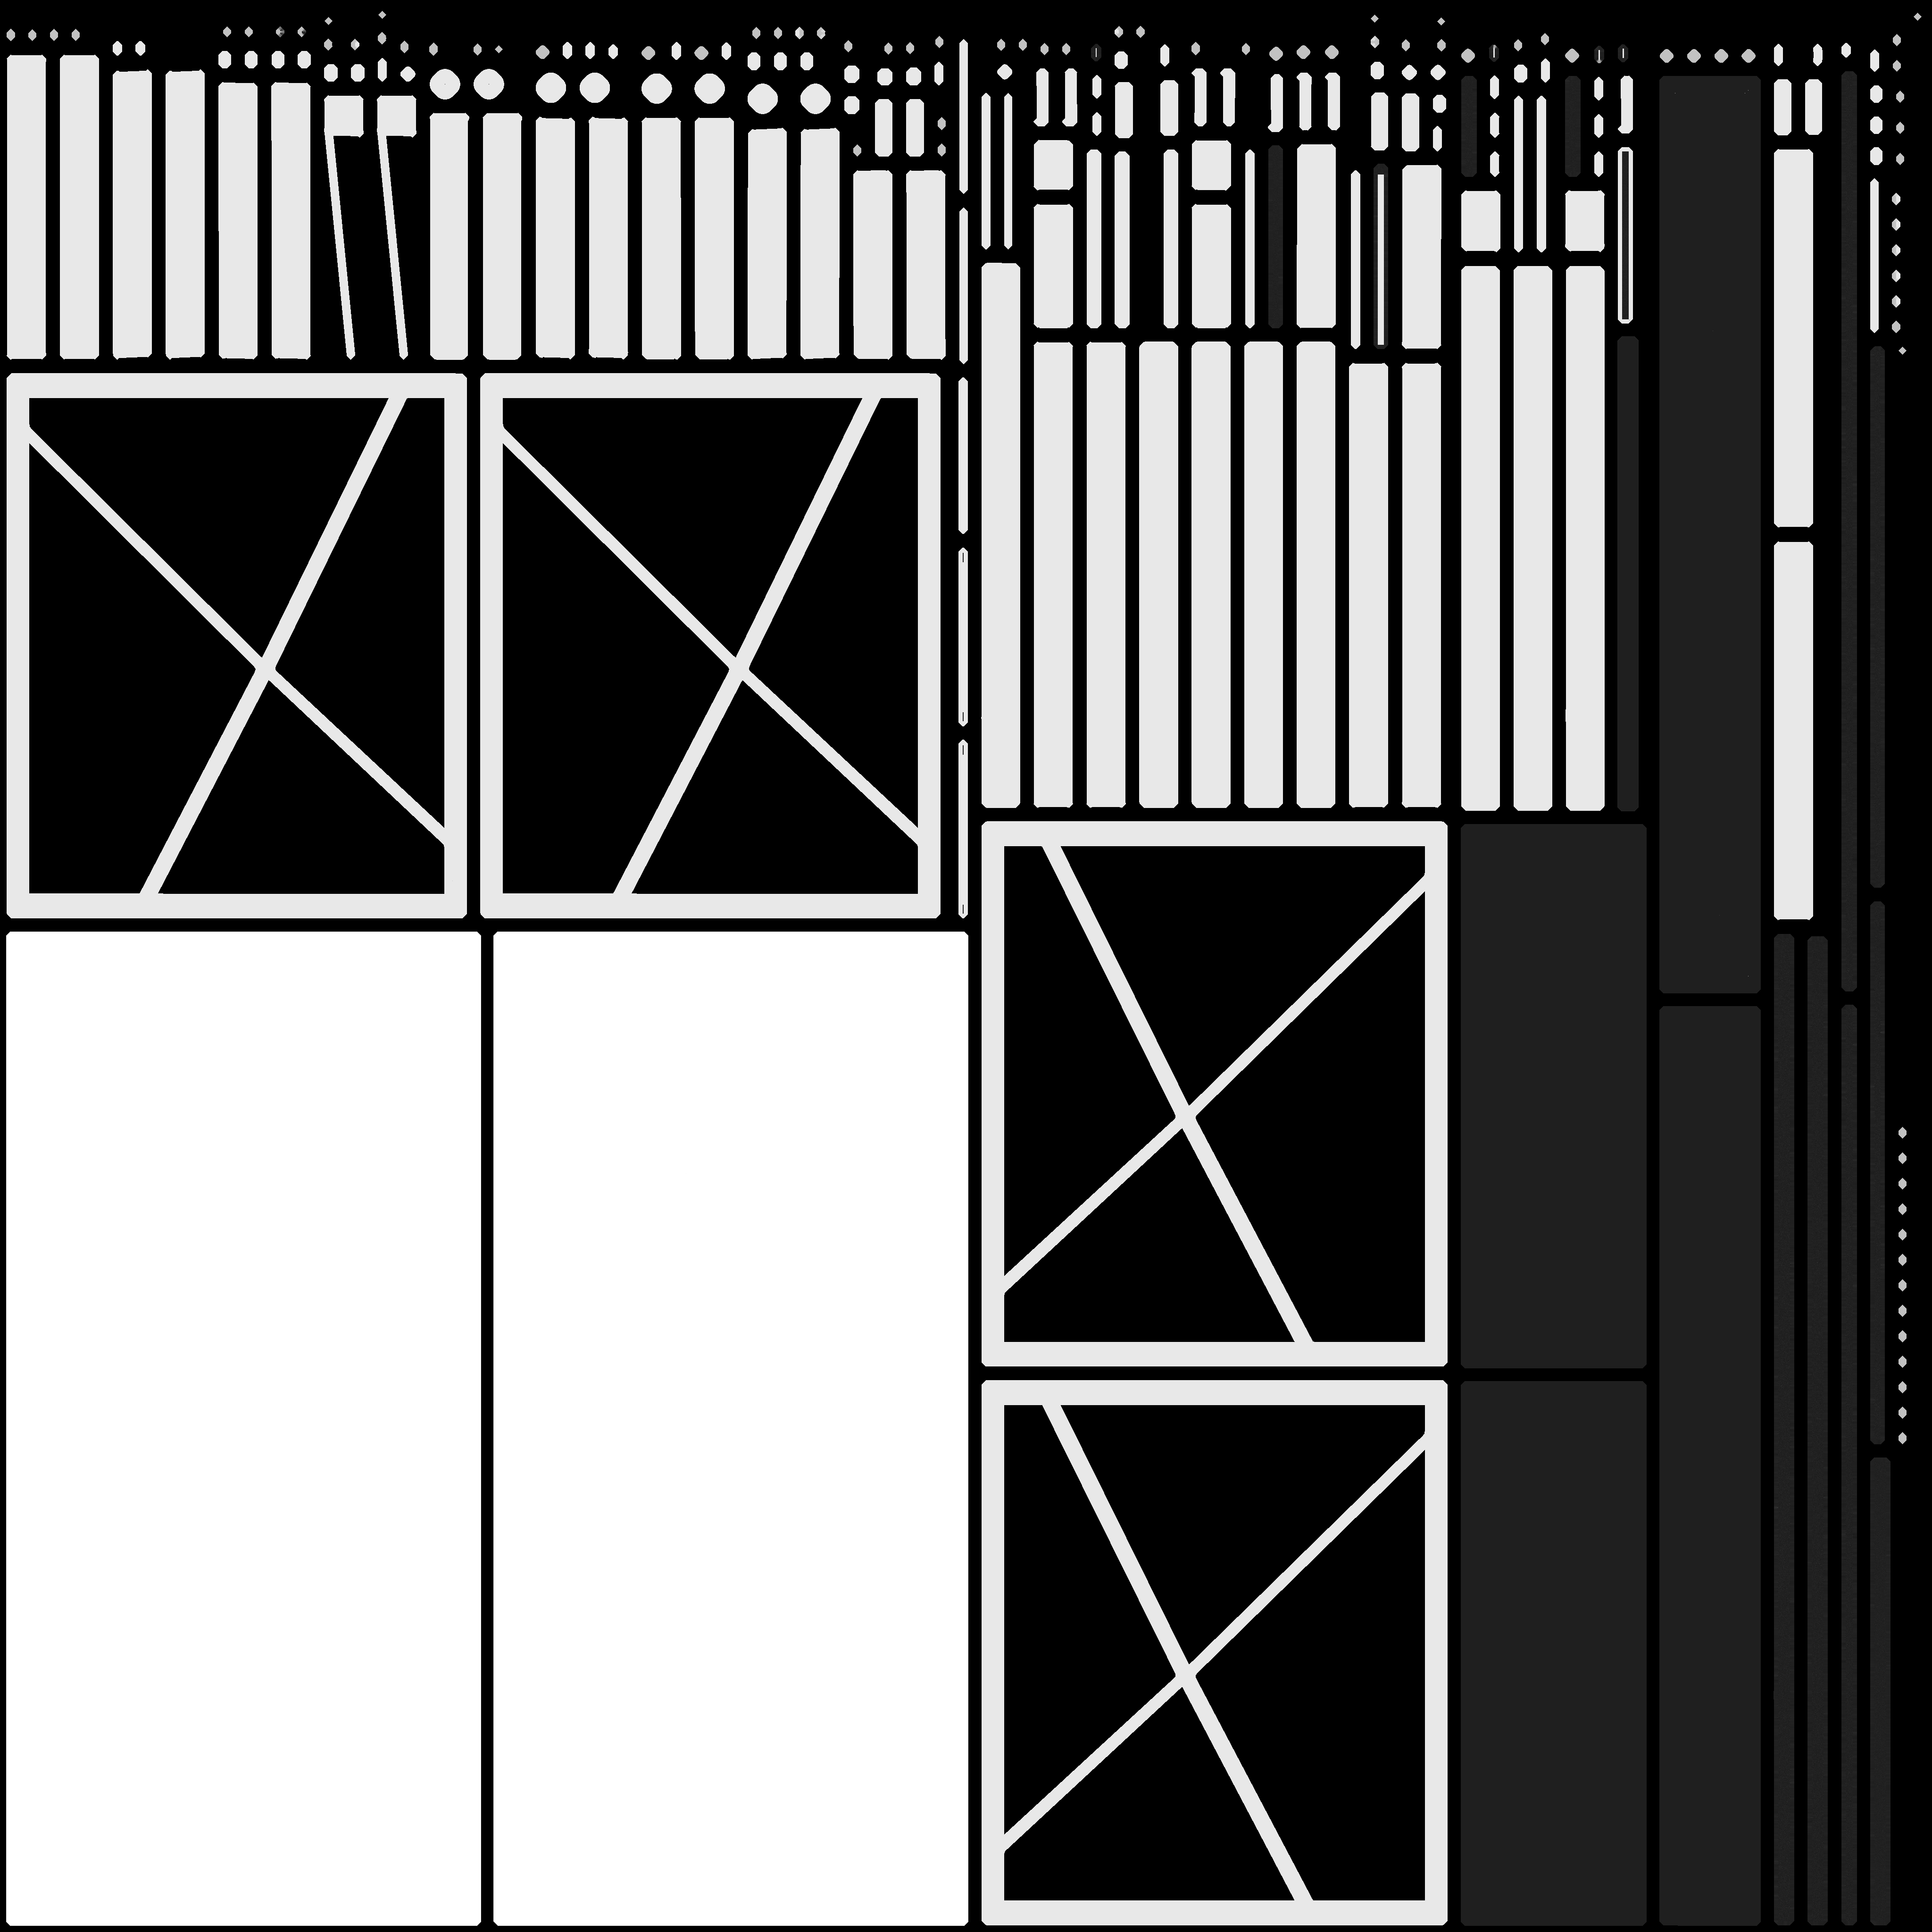
\includegraphics[width=.95\linewidth]{TGF/Artes/pc_desk_albedo2.png}
		\caption{Mapa de UVs del escritorio}
	\end{subfigure}%
	\begin{subfigure}{.5\textwidth}
		\centering
		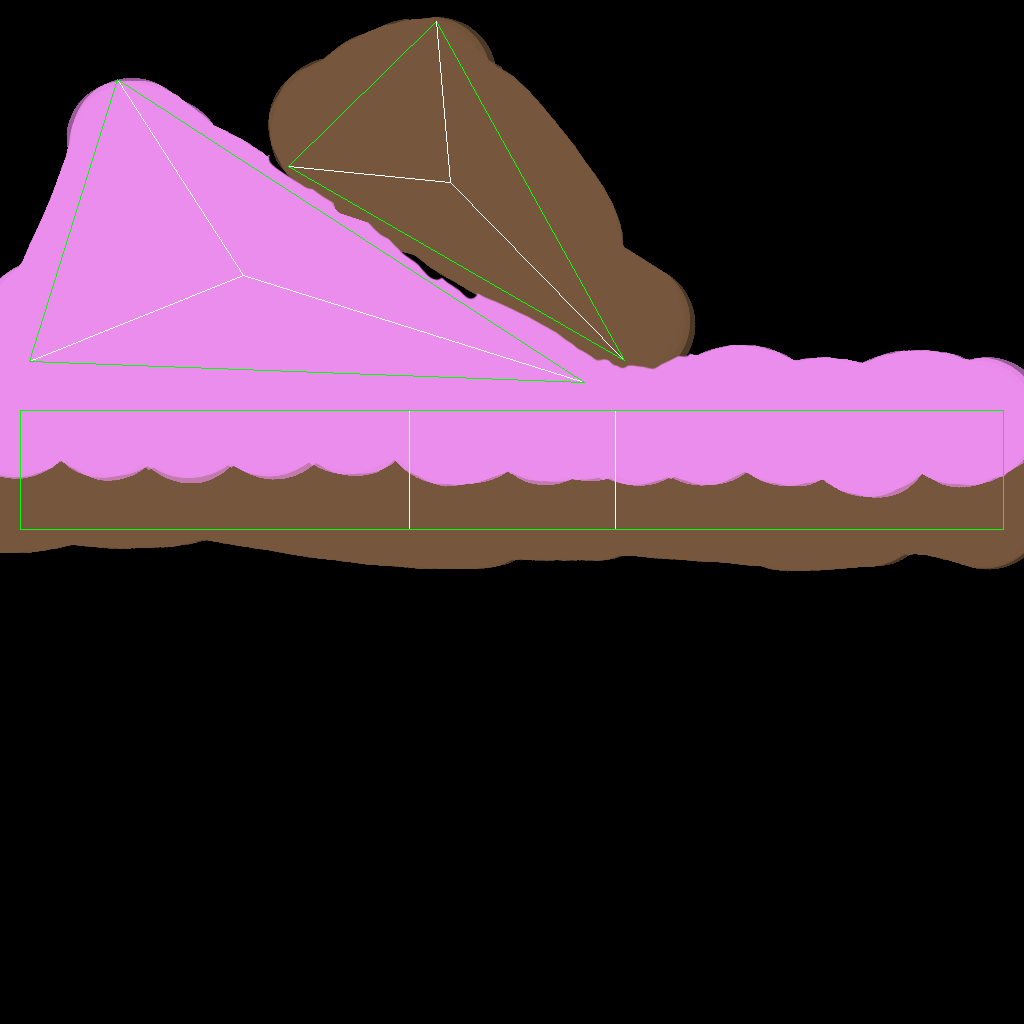
\includegraphics[width=.95\linewidth]{TGF/Artes/Caketext.png}
		\caption{Mapa de UVs de la tarta}
	\end{subfigure}
	\caption{Mapas de UVs}
	\label{fig:texUvs}
\end{figure}

En cuanto a las texturas, en algunos casos se han preservado la de los modelos obtenidos, en otros, o bien se han creado materiales con un color sólido en Unity o se han utilizado texturas externas como en el caso del cuadro, para lo cual se ha utilizado un dibujo realizado por un amigo, \cite{refdibujo}. En otros casos, sin embargo, se ha personalizado las texturas, como en el caso del escritorio o de la cama, como puede verse en la figura \ref{fig:texBed}. Partiendo del mapa de UVs proporcionado por el modelo, se customizó para obtener el resultado deseado. En el caso de la tarta, cuyo modelado se hizo exclusivo para el trabajo, también se realizó un mapa de UVs para texturizarla. Ver Figura \ref{fig:texUvs}. 



\subsubsection{Personajes}
\label{sec:diseñoPersonajes}
Para los personajes, se ha partido de el modelado y animaciones del personaje \citetitle{refCharacter}, así como de las texturas a partir de las cuales se han diseñado la de los personajes utilizados. 

 Personaje 1 - Personaje con TCA 
 
 Mapa de UVs (Ver Figura \ref{fig:ArtesTCA1})
 
 Modelado (Ver Figura \ref{fig:ArtesTCA2})
 
 
 \begin{figure}
\centering
\begin{subfigure}{.5\textwidth}
  \centering
  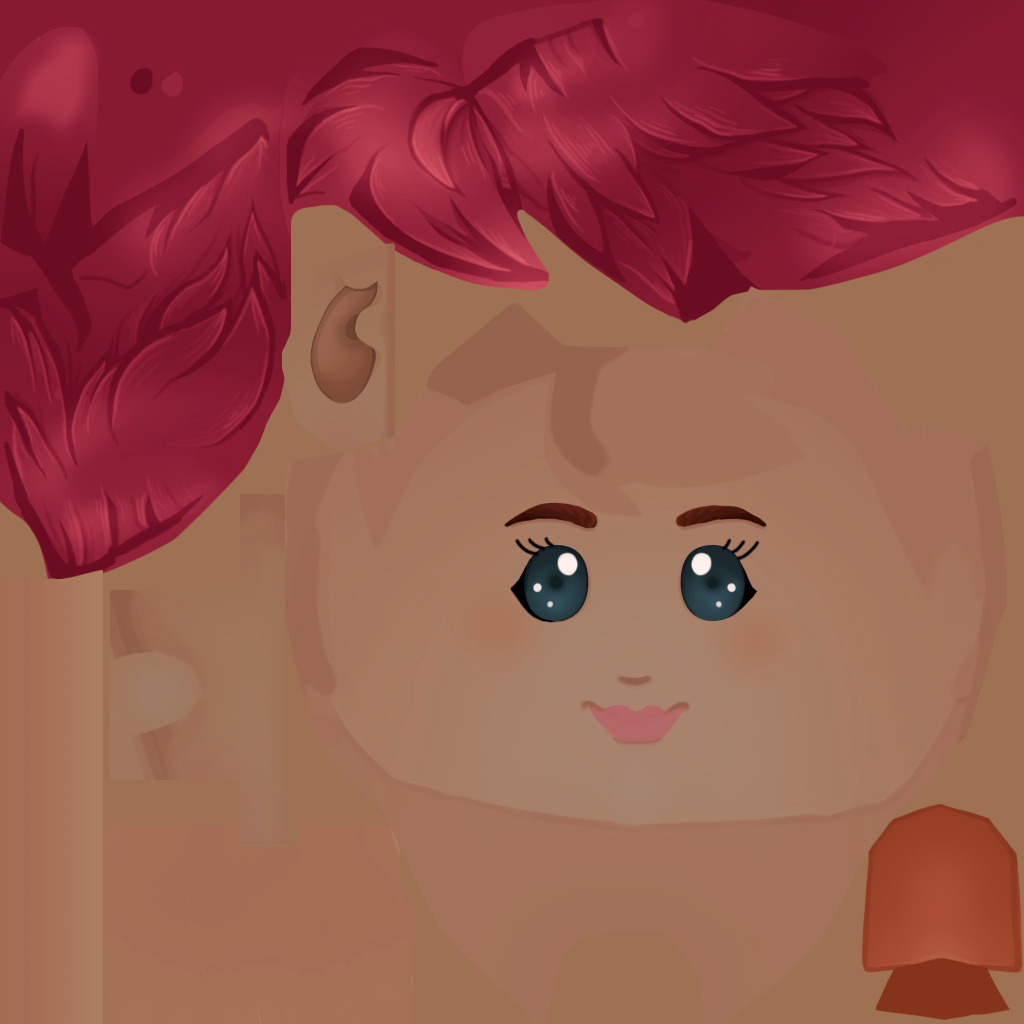
\includegraphics[width=.95\linewidth]{TGF/Artes/TCA_head.png}
  \caption{UV cabeza personaje TCA}
\end{subfigure}%
\begin{subfigure}{.5\textwidth}
  \centering
  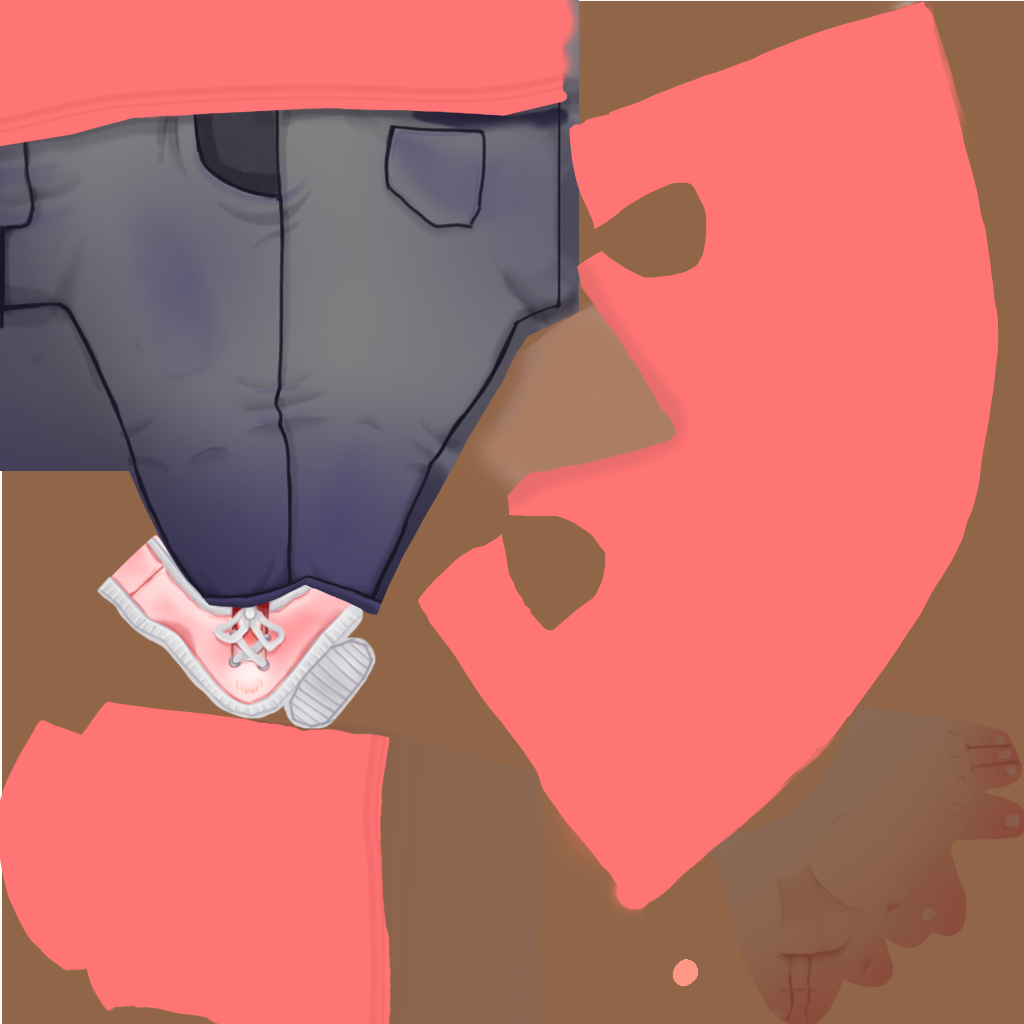
\includegraphics[width=.95\linewidth]{TGF/Artes/TCA_body.png}
  \caption{UV cuerpo personaje TCA}
\end{subfigure}
\caption{UV map persona TCA}
\label{fig:ArtesTCA1}
\end{figure}

 \begin{figure}
\centering
\begin{subfigure}{.5\textwidth}
  \centering
  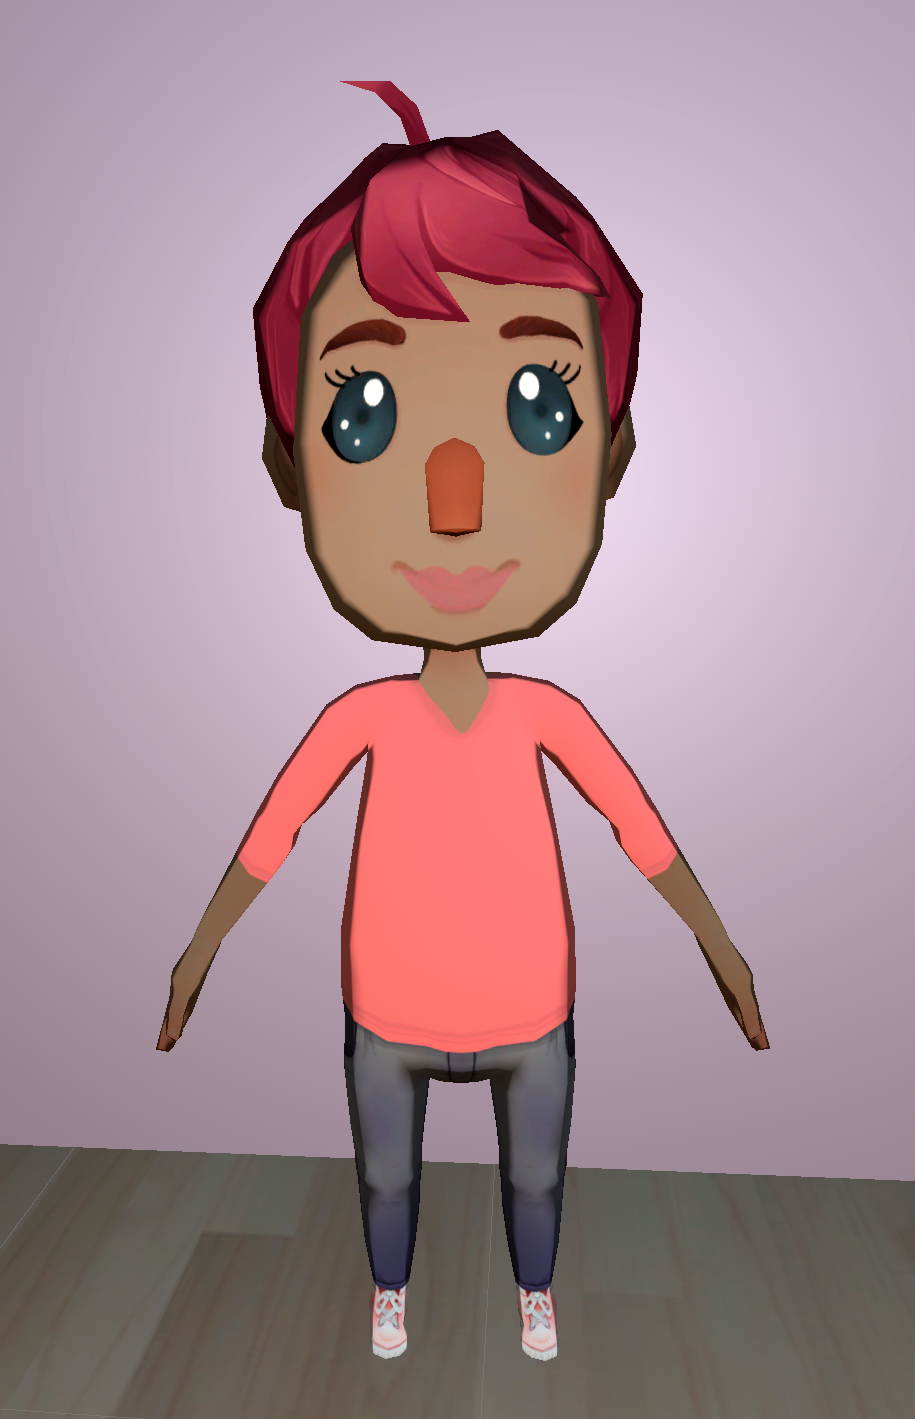
\includegraphics[width=.95\linewidth]{TGF/Artes/TCA_front.png}
  \caption{Personaje TCA frontal}
\end{subfigure}%
\begin{subfigure}{.5\textwidth}
  \centering
  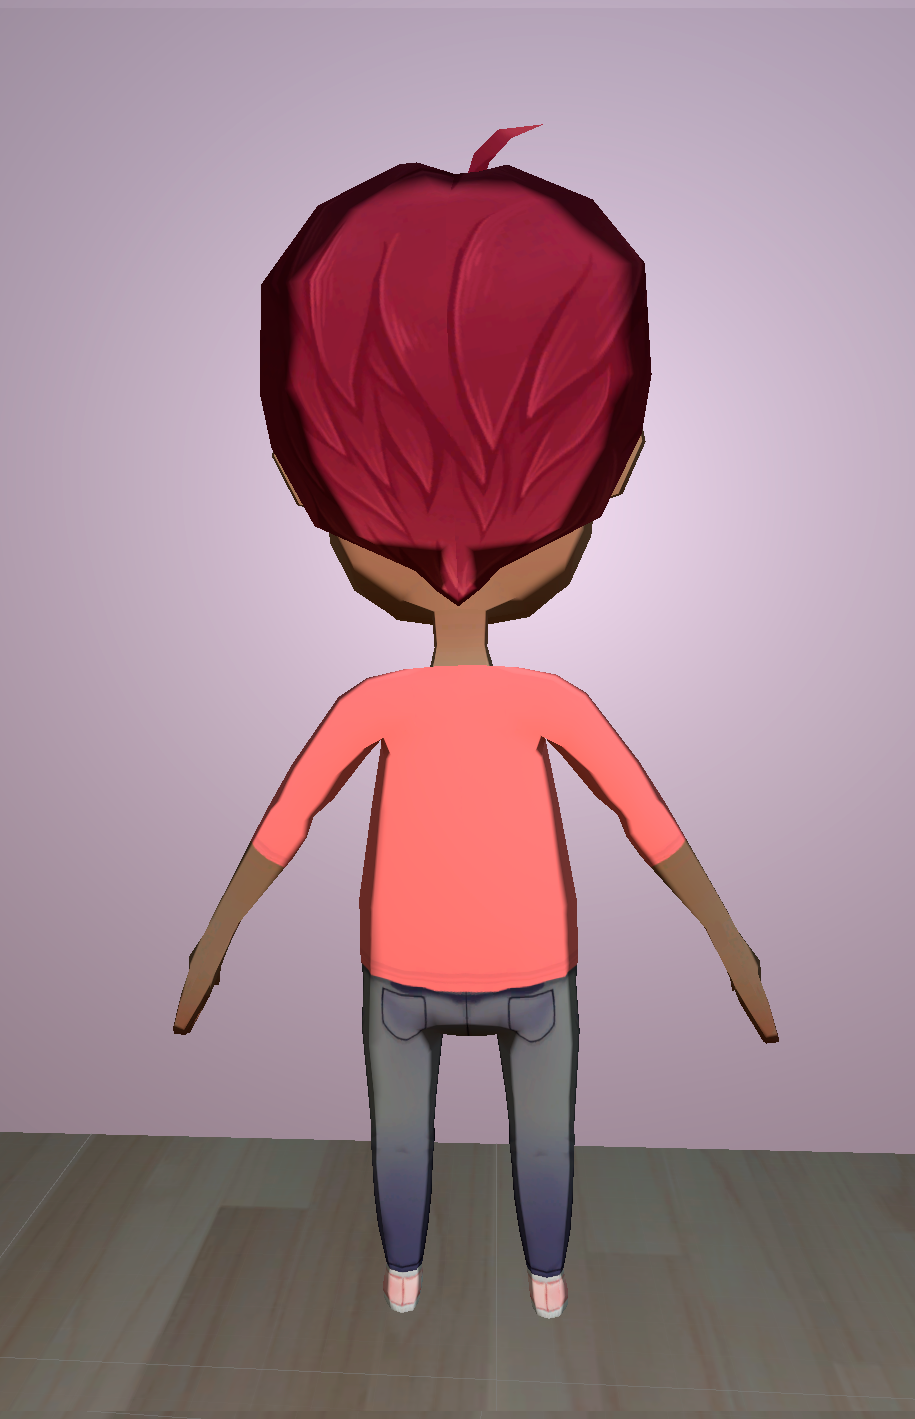
\includegraphics[width=.95\linewidth]{TGF/Artes/TCA_back.png}
  \caption{Personaje TCA de espaldas}
\end{subfigure}
\caption{Personaje TCA}
\label{fig:ArtesTCA2}
\end{figure}


Personaje 2 - Personaje con TAS
 
 Mapa de UVs (Ver Figura \ref{fig:ArtesTAS1})
 
 Modelado (Ver Figura \ref{fig:ArtesTAS2})
 
 
 \begin{figure}
\centering
\begin{subfigure}{.5\textwidth}
  \centering
  \includegraphics[width=.95\linewidth]{TGF/Artes/TAS_head.png}
  \caption{UV cabeza personaje TAS}
\end{subfigure}%
\begin{subfigure}{.5\textwidth}
  \centering
  \includegraphics[width=.95\linewidth]{TGF/Artes/TAS_body.png}
  \caption{UV cuerpo personaje TAS}
\end{subfigure}
\caption{UV map persona TAS}
\label{fig:ArtesTAS1}
\end{figure}

 \begin{figure}
\centering
\begin{subfigure}{.5\textwidth}
  \centering
  \includegraphics[width=.95\linewidth]{TGF/Artes/TAS_front.png}
  \caption{Personaje TAS frontal}
\end{subfigure}%
\begin{subfigure}{.5\textwidth}
  \centering
  \includegraphics[width=.95\linewidth]{TGF/Artes/TAS_back.png}
  \caption{Personaje TAS de espaldas}
\end{subfigure}
\caption{Personaje TAS}
\label{fig:ArtesTAS2}
\end{figure}


Personaje 3 - Personaje con Depresión
 
 Mapa de UVs (Ver Figura \ref{fig:ArtesDEP1})
 
 Modelado (Ver Figura \ref{fig:ArtesDEP2})
 
 \begin{figure}
\centering
\begin{subfigure}{.5\textwidth}
  \centering
  \includegraphics[width=.95\linewidth]{TGF/Artes/DEP_head.png}
  \caption{UV cabeza personaje Depresión}
\end{subfigure}%
\begin{subfigure}{.5\textwidth}
  \centering
  \includegraphics[width=.95\linewidth]{TGF/Artes/DEP_body.png}
  \caption{UV cuerpo personaje Depresión}
\end{subfigure}
\caption{UV map persona Depresión}
\label{fig:ArtesDEP1}
\end{figure}

 \begin{figure}
\centering
\begin{subfigure}{.5\textwidth}
  \centering
  \includegraphics[width=.95\linewidth]{TGF/Artes/DEP_front.png}
  \caption{Personaje Depresión frontal}
\end{subfigure}%
\begin{subfigure}{.5\textwidth}
  \centering
  \includegraphics[width=.95\linewidth]{TGF/Artes/DEP_back.png}
  \caption{Personaje Depresión de espaldas}
\end{subfigure}
\caption{Personaje Depresión}
\label{fig:ArtesDEP2}
\end{figure}


Personajes extra
 
 Mapa de UVs (Ver Figura \ref{fig:ArtesEVIL1})
 
 Modelado (Ver Figura \ref{fig:ArtesEVIL2})
 \begin{figure}
\centering
\begin{subfigure}{.5\textwidth}
  \centering
  \includegraphics[width=.95\linewidth]{TGF/Artes/EVIL_head.png}
  \caption{UV cabeza personaje extra}
\end{subfigure}%
\begin{subfigure}{.5\textwidth}
  \centering
  \includegraphics[width=.95\linewidth]{TGF/Artes/EVIL_body.png}
  \caption{UV cuerpo personaje extra}
\end{subfigure}
\caption{UV map persona extra}
\label{fig:ArtesEVIL1}
\end{figure}

 \begin{figure}
\centering
\begin{subfigure}{.5\textwidth}
  \centering
  \includegraphics[width=.95\linewidth]{TGF/Artes/EVIL_front.png}
  \caption{Personaje extra frontal}
\end{subfigure}%
\begin{subfigure}{.5\textwidth}
  \centering
  \includegraphics[width=.95\linewidth]{TGF/Artes/EVIL_back.png}
  \caption{Personaje extra de espaldas}
\end{subfigure}
\caption{Personaje extra}
\label{fig:ArtesEVIL2}
\end{figure}

\section{Música y efectos de sonido}

Para la música y efectos se sonido se han buscado sinfonías que encajaran con el resto de la temática. Finalmente se encontró un tema principal para ``Insania'' que se va repitiendo en un loop infinito, se trata de \citetitle{music}. 

Por otro lado, se buscaron efectos de sonido acordes a las acciones realizadas por el personaje. En este caso sólo se han añadido efectos para el momento en que se comen pedazos de tarta \citetitle{efectocomer} y cuando se lavan las manos en el lavabo \citetitle{efectoagua}. Podrían incluirse también al escribir una nota en el diario, el click de encender y apagar las luces, o muchos otros sin demasiada complicación. Como se mencionó en la sección \ref{sec:diseñoSw}, simplemente había que añadir nuevos sonidos y añadirlos al array del AudioManager. Una vez están añadidos, se pueden reproducir desde donde se quiera. 

Para que los efectos y la música tuvieran la duración deseada, así como para ajustar el tono, volumen, etc. se utilizó \citetitle{audacity}, de forma que los ajustes realizados desde el propio Unity fueran los mínimos posibles, pequeños ajustes de volumen entre efectos de sonido y música, etc. 

Además, como se indica en el apartado \ref{sec:encuestaDemo}, se añadieron controles para pausar o continuar reproduciendo la música en el menú de pausa, dado que algunos de los encuestados consideraban que era un elemento importante dado que había a quienes les sacaba de la experiencia jugable escuchar la misma música continuamente. 



\chapter {Evaluación}

\section{Encuestra sobre videojuegos y enfermedades mentales}
\label{sec:encuestaVid}
Aparte de los estudios que se han encontrado acerca de la representación de los trastornos y enfemedades mentales en videojuegos así como en otros medios, se ha realizado un estudio propio. Para ello se ha realizado una encuesta que se ha distribuido, obteniendo un total de 254 respuestas. Esta encuesta ha sido realizada tanto en castellano como en inglés, llegando así a una mayor parte de la población.De las respuestas obtenidas, un total de 198 respuestas se han obtenido de la encuesta en castellano y 56 de la encuesta realizada en inglés. En cuanto a su distribución, se han utilizado medios como Twitter, Instagram, contactos personales, o Reddit (en subreddits donde se habla de videojuegos, enfermedades mentales y de encuestas en general). 

Para la encuesta se han tenido en consideración varias cosas. En primer lugar, la encuesta se ha estructurado con 9 secciones diferentes excluyentes. Algunas preguntas hacen al usuario navegar hacia la sección siguiente o saltarse las que ya no tiene que responder. Por ejemplo, una pregunta sobre si tienen conocimiento de algún videojuego que represente una enfermedad contestada de forma negativa evitará que naveguen por el resto de preguntas sobre ese tema, en las cuales se profundiza más. Otra consideración ha sido a la hora de escoger el rango de respuestas posibles. Se ha escogido un rango de número par, evitando así que un gran número de personas escojan el punto central para no tener que decantarse hacia un lado u otro. De ese modo las respuestas generalmente han sido ``Nada-Poco-Algo-Mucho'', o términos similares, en función de la pregunta. 

Analizando ahora cada una de las secciones de la encuesta, en primer lugar se encuentra la sección de introducción y consentimiento. En el caso de no aceptarse ese consentimiento, se trasladará al final de la encuesta animando a participar en otro momento. En el caso de responder de forma afirmativa, se continúa con la siguiente sección. Esta siguiente sección es un control demográfico donde se pregunta por el género (Femenino-Masculino-No binario-Otro), para poder hacer un análisis sobre un mayor conocimiento o sensibilidad sobre las enfermedades mentales en cada uno de los casos. La edad ha sido dividia en seis rangos diferentes (10-19, 20-29, 30-39, 40-49,50-65, 65+). Ninguna de estas preguntas eran de caracter obligatorio. Posteriormente se pregunta sobre la frecuencia con que juegan a videojuegos y el tipo de videojuegos. Esto puede ayudarnos a prestar especial atención a las respuestas de personas que jueguen más o a determinado tipo de videojuegos, dado que quienes únicamente juegan al ajedrez pueden desconocer la existencia de videojuegos donde estén presentes enfermedades mentales. 

La tercera sección consiste en preguntas acerca de la representación en diferentes medios, como películas, series o videojuegos, pudiéndose escoger de Nada a Mucho así como el conocimiento que consideran tener sobre diferentes enfermedades mentales. De este modo también ayudará a saber la fidelidad de otras respuestas acerca de enfermedades en videojuegos, en el caso de conocer alguno. Esta es la siguiente pregunta, si se tiene constancia de algún videojuego donde se represente alguna enfermedad mental. En el caso de obtener una respuesta negativa se saltará de sección, mientras que en caso afirmativo se preguntará sobre qué videojuegos conoce, qué enfermedades representan estos, y la percepción que tienen en cuanto a cómo es esa representación. Se cuestiona sobre cuánto creen que mantienen el estigma, si conocen videojuegos donde se representen de forma correcta y cuáles, y cómo de fiel consideran que suele ser la representación y si creen que está variando con el tiempo la forma de representar las enfermedades mentales. 

Las últimas secciones están más centradas en enfermedades mentales, se pregunta primero si el encuestado tiene o cree tener algún trastorno o enfermedad mental para redirigir o no a preguntas concretas sobre el tema. Entre estas se encuentran si las enfermedades están diagnsoticadas, de qué enfermedades se trata y si conocen algún videojuego donde se represente. Esta es la última pregunta donde se ramifican los caminos en función de la respuesta obtenida. Quien no conozca ningún videojuego acabará la encuesta añadiendo observaciones o un saludo, mientras que quien sí conozca primero indicará cuáles son, en qué medida se ha sentido representado por ellos y por qué y cómo creen que podrían haber sentido mejor la representación. 


El link a la encuesta en castellano puede encontrarse en \citetitle{encuestaVidESP}, la encuesta en inglés podrá encontrarse en \citetitle{encuestaVidING}.

%%%%%%%%%%%%%%%%%%%%%%%Resultados encuesta%%%%%%%%%%%%%%%%%%%%%%%%%%%%%%
\subsection{Resultados obtenidos}


Haciendo un análisis del conjunto de respuestas, se han obtenido un total de 254 respuestas. Sólo dos personas no respondieron a la pregunta sobre el género, de los encuestados restantes, 129 de las respuestas se corresponden con personas de género masculino, 112 de género femenino y finalmente 11 de género no binario. 198 de las respuestas obtenidas se han recogido de la encuesta en castellano (ver Figura \ref{fig:ESPGen}), perteneciendo las 56 restantes a la encuesta en inglés (ver Figura \ref{fig:INGGen}). 
La edad de los encuestados generalmente se ha encontrado entre el rango de los 20 a los 29 años, seguido de los 50-65 y 10-19. Sin embargo, como puede observarse, se ha recogido una muestra bastante diversa. (Veánse las figuras \ref{fig:GenAge}). 



\begin{figure}
\centering
\begin{subfigure}{.5\textwidth}
  \centering
  \includegraphics[width=.9\linewidth]{Imagenes Form GEN/1GENGenre}
  \caption{GEN: Género}
\end{subfigure}%
\begin{subfigure}{.5\textwidth}
  \centering
  \includegraphics[width=.9\linewidth]{Imagenes Form GEN/2GENAge}
  \caption{GEN: Edad}
\end{subfigure}
\caption{GEN:Control demográfico}
\label{fig:GenAge}
\end{figure}

En la frecuencia de juego podemos encontrar todo tipo de jugadores, desde los más frecuentes a los que juegan poco o prácticamente nada, encontrándose la media en un valor de 3,5 en una escala del 1 al 6 y la mediana en el valor 4, (ver Figura \ref{fig:Frec}). Se encuentra una mayor frecuencia entre los encuestados en la encuesta en inglés (ver Figura \ref{fig:INGFrec}) que en la de castellano (ver Figura \ref{fig:ESPFrec}).

\begin{figure}
\centering
 \includegraphics[width=.7\linewidth]{Imagenes Form GEN/3GENFrec}
 \caption{GEN: Frecuencia de juego}
 \label{fig:Frec}
 \end{figure}
 
En cuanto a los géneros de videojuego a los que más encuestados juegan son de simulación (Los Sims, Animal Crossing, etc.), seguidos de los juegos de aventura (The Last of Us, Death Stranding, etc.)  y RPGs (Dark Souls, GTA, etc.). (Ver Figura \ref{fig:Frecgen}). 

En este caso en castellano, se encontraban más jugadores de juegos de simulación, seguidos de los de plataformas (Mario Bros, Crash Bandicoot, etc.), aventura y puzles (Candy Crush, Portal, etc.) (ver Figura \ref{fig:ESPFrecgen}). Sin embargo, en la encuesta en inglés, los más jugados eran los de RPG seguidos de los de aventura y simulación (ver Figura \ref{fig:INGFrecgen}).  


\begin{figure}
\centering
 \includegraphics[width=.8\linewidth]{Imagenes Form GEN/4GENGen}
 \caption{GEN: Frecuencia por género de juego \\
 \small{N(No juego a videojuegos); A(Aventura); B(Battle Royale); D(“Defender la torre”); De(Deportivos); E(Estrategia); G(Gestión); H(Hack and Slash); M(Musicales); L(Lucha); Me(Metroidvania); Mm(MMORPG); Mo(MOBA); P(Plataformas); Pu(Puzzles); R(RPG); Ro(Rogue Like); S(Shooters); Si(Simulación); Su(Supervivencia); T(Terror); O(Otros)}}
 \label{fig:Frecgen}
 \end{figure}
 
 Distinguiendo entre los géneros más jugados por los jugadores con frecuencia de juego de nivel 5 o 6, formado por un total de 80 personas, los juegos más jugados pertenecen a los géneros de RPG y aventuras (ver Figura \ref{fig:Frecgen56}). Se puede llegar a la conclusión de que los juegos de simulación o puzles son jugados por jugadores más casuales. 
 
 \begin{figure}
\centering
 \includegraphics[width=.8\linewidth]{ANEXO Gen/8AnexGENFrecgen56}
 \caption{GEN: Frecuencia por género de juego; jugadores con frecuencia de juego nivel 5-6}
 \label{fig:Frecgen56}
 \end{figure}
 
 
La representación de las enfermedades mentales en medios al unificar las respuestas de ambos cuestionarios indica que la gran mayoría opina que hay “Algo” de representación en películas, series y los libros y “Poca” en las noticias y los videojuegos. (Ver Figura \ref{fig:Medios}). 

Cabe destacar que el medio en el que más se considera que no tiene representación son los videojuegos y el medio donde se considera que hay mayor representación de las enfermedades mentales, los libros. 

Los resultados en este caso son bastante similares en ambos cuestionarios, las mayores diferencias se encuentran en la representación en videojuegos, donde mucha más gente en la encuesta en castellano (ver Figura \ref{fig:ESPMedios}) considera que no hay nada de representación. Por otro lado, en la encuesta en inglés (ver Figura \ref{fig:INGMedios}) consideran que en los libros hay más representación de las enfermedades mentales. 


\begin{figure}
\centering
 \includegraphics[width=.9\linewidth]{Imagenes Form GEN/5GENMedio}
 \caption{GEN: Representación de enfermedades mentales en medios}
 \label{fig:Medios}
 \end{figure}

En cuanto al conocimiento sobre los diferentes trastornos mentales, a excepción del TEPT, los TPs y los TDs, cuya gran mayoría de personas considera que sabe “Poco”, sobre el resto de enfermedades los encuestados afirman saber “Algo” (ver Figura \ref{fig:Conocimiento}). 

Los trastornos de los que más conocen son los TEAn (depresión, trastorno de bipolaridad, etc.), y los más desconocidos, los TDs (trastorno de identidad disociativo, trastorno de despersonalización-desrealización, etc.). 

En este caso, en la encuesta en inglés generalmente los encuestados conocían más sobre los diferentes trastornos o enfermedades mentales (ver Figura \ref{fig:INGCon}). Conocen más sobre algunos trastornos como el TAG o el TEPT. Mientras que en castellano prácticamente un 20\% consideraba no saber nada sobre el TAG en esta todo el mundo sabe al menos un poco sobre él. Podría decirse que en términos generales conocen más sobre todas las enfermedades presentadas (ver Figura \ref{fig:ESPCon}). 


\begin{figure}
\centering
 \includegraphics[width=1\linewidth]{Imagenes Form GEN/6GENCon}
 \caption{GEN: Conocimiento sobre trastornos mentales\\
 TAG (Trastorno de Ansiedad Generalizada); TOC (Trastorno Obsesivo Compulsivo); TAS(Trastorno de Ansiedad Social); TEAn(Trastornos del Estado del Ánimo); TCA(Trastornos de la Conducta Alimentaria); TEPT (Trastorno de Estrés Post-Traumático); TP (Trastornos Psicóticos); TD (Trastornos Disociativos) }
 \label{fig:Conocimiento}
 \end{figure}


Haciendo una distinción entre géneros, es también relevante la diferencia del conocimiento sobre determinadas enfermedades en función de este. En términos generales, las encuestadas de género femenino, un total de 131 personas, consideran que saben “Algo” sobre todos los trastornos a excepción de los TPs y TDs, de los cuales consideran que saben “Poco” (ver Figura \ref{fig:Confem}). 

En las diferentes encuestas puede observarse que en la encuesta en castellano (ver Figura \ref{fig:ESPConfem}), aparte de por ser una muestra mayor, hay más personas que consideran no saber nada sobre todas las enfermedades mentales. Sin embargo, en el caso de la encuesta en inglés (ver Figura \ref{fig:INGConfem}) todas las encuestadas conocen al menos algo sobre el TAG, TOC, TAS, TEAn, TCAs y TEPT. Podría decirse que generalmente conocen más sobre las enfermedades mentales. No obstante, en el caso de las adicciones más encuestadas en castellano consideran saber más que en la encuesta en inglés. 


\begin{figure}
\centering
 \includegraphics[width=1\linewidth]{ANEXO Gen/11AnexGENCongfem}
 \caption{GEN: Conocimiento sobre trastornos mentales - Género femenino\\
 TAG (Trastorno de Ansiedad Generalizada); TOC (Trastorno Obsesivo Compulsivo); TAS(Trastorno de Ansiedad Social); TEAn(Trastornos del Estado del Ánimo); TCA(Trastornos de la Conducta Alimentaria); TEPT (Trastorno de Estrés Post-Traumático); TP (Trastornos Psicóticos); TD (Trastornos Disociativos) }
 \label{fig:Confem}
 \end{figure}



Sin embargo, los encuestados de género masculino, un total de 108 personas, consideran que saben “Poco” sobre el TAG, TEPT, TPs y TDs, y “Algo” sobre el resto de enfermedades. Generalmente, además, conocen menos sobre todas las enfermedades presentadas a excepción de las adicciones, donde sólo un encuestado dice no saber nada (ver Figura \ref{fig:Conmasc}). 

Esta diferenciación se acentúa también entre las diferentes encuestas. En la encuesta en castellano, (ver Figura \ref{fig:ESPConmasc}),  muchos de los encuestados consideran saber poco o nada sobre el TAG, el TAS, mientras que son enfermedades conocida por todos los encuestados en inglés y en el caso del TAS, bastante conocida. Por otro lado, cabe destacar también que en la encuesta en inglés (ver Figura \ref{fig:INGConmasc}), la mediana sobre el conocimiento sobre los TEAn se encuentra en “Mucho”. Es decir, la mayoría de los encuestados conocen mucho sobre este tipo de trastornos, mientras que en la encuesta en castellano, saben “Algo” o “Poco”, generalmente. 


\begin{figure}
\centering
 \includegraphics[width=1\linewidth]{ANEXO Gen/12AnexGENCongmasc}
 \caption{GEN: Conocimiento sobre trastornos mentales - Género masculino\\
 TAG (Trastorno de Ansiedad Generalizada); TOC (Trastorno Obsesivo Compulsivo); TAS(Trastorno de Ansiedad Social); TEAn(Trastornos del Estado del Ánimo); TCA(Trastornos de la Conducta Alimentaria); TEPT (Trastorno de Estrés Post-Traumático); TP (Trastornos Psicóticos); TD (Trastornos Disociativos) }
 \label{fig:Conmasc}
 \end{figure}

En el caso de los encuestados de género no binario, y teniendo en cuenta que la muestra es de tan sólo 11 personas, generalmente conocen más sobre todas las enfermedades mentales, encontrándose las medianas en el nivel “Algo” en todas las enfermedades a excepción de los TDs, que se encuentra en “Poco”. (Ver Figura \ref{fig:Conbn}). 

En este caso, la diferenciación entre encuestas no tiene sentido por el tamaño de la muestra en ambos casos, pero más o menos es similar, como puede verse en las gráficas en castellano y en inglés (ver Figuras \ref{fig:ESPConnb} y \ref{fig:INGConnb}). 


\begin{figure}
\centering
 \includegraphics[width=1\linewidth]{ANEXO Gen/13AnexGENConnb}
 \caption{GEN: Conocimiento sobre trastornos mentales - Género no binario\\
 TAG (Trastorno de Ansiedad Generalizada); TOC (Trastorno Obsesivo Compulsivo); TAS(Trastorno de Ansiedad Social); TEAn(Trastornos del Estado del Ánimo); TCA(Trastornos de la Conducta Alimentaria); TEPT (Trastorno de Estrés Post-Traumático); TP (Trastornos Psicóticos); TD (Trastornos Disociativos) }
 \label{fig:Conbn}
 \end{figure}


%%%%%%%Videojuegos y enfermedades mentales%%%%%%%%%%%%

 Pasando a la sección de videojuegos y enfermedades mentales, sólo un 30\% de los encuestados conoce videojuegos donde se trate el tema de las enfermedades mentales (ver Figura \ref{fig:GENConvid}). La figura  \ref{fig:ESPConvid} muestra los resultados de la encuesta en español, donde se observa que este porcentaje es de un 29\%, respectivamente, en la encuesta en inglés, se puede ver en la figura \ref{fig:INGConvid}, que el porcentaje es de un 36\%. 
 %%\comm{¿Por qué la Figura~\ref{fig:ESPConvid} está en el anexo y la Figura~\ref{fig:INGConvid} no?}%

%%\commin{La Figura~\ref{fig:ESPConvid}  muestra los resultados de la encuesta en español (resp. la Figura ??? de la encuesta en inglés) donde se observa que este porcentaje es de un 29\% (resp. un 36\%).}


Entre las enfermedades que se consideran mayoritariamente representadas están, en primer lugar la depresión, coincidente en ambas encuestas, seguida de los TPs y el TEPT. Por otro lado, los TCAs son los trastornos que menos se ven representados.  

Haciendo una distinción entre ambas encuestas, en la encuesta en castellano más gente conoce videojuegos donde se representan diferentes enfermedades como las adicciones, mientras que en la encuesta en inglés nadie conoce ninguno, el TB o las fobias. 

\begin{figure}
\centering
\begin{subfigure}{.4\textwidth}
  \centering
  \includegraphics[width=.95\linewidth]{Imagenes Form GEN/7GENConenf}
  \caption{GEN: Conocimiento de videojuegos donde se representan enfermedades mentales}
\end{subfigure}%
\begin{subfigure}{.6\textwidth}
  \centering
  \includegraphics[width=.95\linewidth]{Imagenes Form GEN/8GENConenf}
  \caption{GEN: Enfermedades mentales representadas en videojuegos}
\end{subfigure}
\caption{GEN:Videojuegos y enfermedades mentales}
\label{fig:GENConvid}
\end{figure}

En el caso de los jugadores con nivel de frecuencia 5 o 6, que consiste de una muestra de 80 personas, el 50\% conoce videojuegos donde se representan enfermedades mentales, manteniéndose prácticamente la proporción en cuanto a las enfermedades representadas (ver Figura \ref{fig:Convid56}).


\begin{figure}
\centering
\begin{subfigure}{.4\textwidth}
  \centering
  \includegraphics[width=.95\linewidth]{Imagenes Form GEN/7GENConenf}
  \caption{GEN: Conocimiento de videojuegos donde se representan enfermedades mentales}
\end{subfigure}%
\begin{subfigure}{.6\textwidth}
  \centering
  \includegraphics[width=.95\linewidth]{Imagenes Form GEN/8GENConenf}
  \caption{GEN: Enfermedades mentales representadas en videojuegos}
\end{subfigure}
\caption{GEN:Videojuegos y enfermedades mentales; Jugadores con frencuencia de juego nivel 5-6}
\label{fig:Convid56}
\end{figure}

Entre estos videojuegos que representan enfermedades mentales se encuentran algunos como \citetitle{alice11}, \citetitle{franbow15}, \citetitle{daysgone19}, \citetitle{hellblade17}, \citetitle{lifeisstrange18} o \citetitle{gris18}. El listado completo se encuentra en el Anexo~\ref{sec:listadoVid}.
%%\comm{JAH: coloca el label a continuación de subsection y referencia el anexo}
%\hyperref[listadoVid]{anexo}.\\
   
En cuanto al estigma que sigue existiendo en los medios acerca de las enfermedades mentales, consideran que se sigue preservando en cierto modo, obteniendo como resultados una media de 2,22 y una mediana en el valor 2 en una escala del 1 al 4 (ver Figura \ref{fig:Estigma}). 

%%\comm{Añadir ``Figura'' para explicar que es la referencia, aquí puedes poner ``(ver Figura 6.12)''}\ref{fig:Estigma}. 

Estos resultados son muy similares en ambas encuestas, ver Figuras~\ref{fig:ESPEstigma} y \ref{fig:INGEstigma}.  

%%\comm{En este punto he añadido ``ver Figuras'' para que veas la diferencia}


\begin{figure}
\centering
 \includegraphics[width=.8\linewidth]{Imagenes Form GEN/9GENEstg}
 \caption{GEN: Nivel de preservación del estigma sobre las enfermedades mentales en videojuegos}
 \label{fig:Estigma}
 \end{figure}
 
Algunas de las justificaciones a estas respuestas en la encuesta en castellano:

\textit{``No creo que estigmaticen, si está bien hecho te ayudan a empatizar con la psicopatología del/de la protagonista''} (nivel 1)

\textit{``La representación es exageradamente estereotipada.''} (nivel 3) 

\textit{``En los juegos de terror o los villanos suelen tener enfermedades mentales''} (nivel 3)

\textit{``Dando a representar a personas enfermas como locos o personas que no se pueden controlar''} (nivel 4) 

Se pueden encontrar el resto de respuestas en el \hyperref[estigmaCastellano]{anexo}.

En el caso de la encuesta en inglés, algunas de las justificaciones son las siguientes:

\textit{``I don't think they do. To a large extent, due to the interactive nature, there is more approach, which if any way reduces stigma.}'' (nivel 1) (No creo que lo hagan. En gran medida, debido a la naturaleza interactiva, hay un mayor enfoque, que de algún modo, reduce el estigma)  

\textit{``They promote the stereotype of those illnesses''} (nivel 3) (Promueven el estereotipo de esas enfermedades)

\textit{``Tend to use sensationalized extreme cases of the mental disorder''} (nivel 3) (Tienden a utilizar casos extremos y sensacionalistas del trastorno mental)

\textit{``They often make the mentally ill characters violent enemies''} (nivel 3) (Normalmente hacen a los personajes con enfermedades mentales, enemigos violentos)

El resto de las respuestas pueden encontrarse en el \hyperref[estigmaIngles]{anexo}.

Como puede verse, hay gran diversidad de opiniones, desde gente que considera que pueden utilizarse como una herramienta para desestigmatizar, precisamente, y otros que ven que actualmente sólo se utiliza para justificar la violencia de los enemigos o utilizar estereotipos de dichas enfermedades. 

Entre los participantes que conocían videojuegos donde se representaran enfermedades mentales, un total de 77 personas, un 42\% de ellos conocen videojuegos que consideran que estas se representan correctamente. (Ver Figura \ref{fig:Enfvid}). 

En este caso las respuestas son muy diferentes en el caso de ambas encuestas, donde en la encuesta en castellano este porcentaje es de un 35\% y en la encuesta en inglés, de un 60\%. (Ver Figuras \ref{fig:ESPCorr} y \ref{fig:INGCorr}). 

 Entre estos videojuegos se encuentran algunos de los mencionados anteriormente como \citetitle{lifeisstrange18} o \citetitle{gris18} y algunos otros como \citetitle{night17}, \citetitle{thecat12} o \citetitle{celeste18}. El listado completo se encuentra en el \hyperref[listadoVidCorr]{anexo}\\ 
 
Por otro lado, generalmente consideran que la fidelidad en cuanto a la representación de las enfermedades mentales se encuentra en un nivel 3 en una escala del 1 al 6, estando la media en 3,14. En este caso sí que coinciden bastante en ambas encuestas con las respuestas, manteniéndose prácticamente la misma proporción en ambos casos. 



\begin{figure}
\centering
\begin{subfigure}{.4\textwidth}
  \centering
  \includegraphics[width=.95\linewidth]{Imagenes Form GEN/10GENCorr}
  \caption{GEN: Conocimiento de videojuegos donde se representan enfermedades mentales correctamente}
\end{subfigure}%
\begin{subfigure}{.6\textwidth}
  \centering
  \includegraphics[width=.95\linewidth]{Imagenes Form GEN/11GENFid}
  \caption{GEN: Enfermedades mentales representadas correctamente en videojuegos}
\end{subfigure}
\caption{GEN:Representación correcta de enfermedades mentales en videojuegos}
\label{fig:Enfvid}
\end{figure}

De entre estos encuestados que conocen videojuegos donde se traten las enfermedades mentales, un total de 77 respuestas, aproximadamente un 60\% de ellos considera que con el tiempo existirá una mejor representación de las enfermedades mentales, (ver Figura \ref{fig:Mejor}), manteniéndose una proporción similar en el caso de la encuesta en castellano y en inglés (ver Figuras \ref{fig:ESPMejor} y \ref{fig:INGMejor}). 

\begin{figure}
\centering
 \includegraphics[width=.8\linewidth]{Imagenes Form GEN/12GENMejor}
 \caption{GEN: Mejor representación de las enfermedades mentales en videojuegos en el futuro}
 \label{fig:Mejor}
 \end{figure}

Entre las justificaciones con respecto a estas respuestas, en castellano podemos encontrar algunas como: 

\textit{``En general se le está dando más visibilidad a la salud mental que hace una/dos décadas y eso repercute en toda forma artística ya sea música, películas, series, teatro, videojuegos…''} (Sí)

\textit{``La aparición de nuevos estudios abre las puertas al incremento de la riqueza en cuanto a la temática de los videojuegos.''} (Sí)

\textit{``Creo que especialmente el mundo de los indies, con desarrolladores más jóvenes, visiones más personales y uso del ``art game'' como forma de expresión y no solo ocio, suponen una plataforma que poquito a poco se está usando''.} (Sí)

\textit{``No tengo mucha confianza en que los AAA salgan de su estanca visibilidad en relación a las enfermedades mentales, ya que son mainstream y no se arriesgan. Por otro lado, sí tengo confianza en los juegos indie, ya que se arriesgan y hacen historias magníficas, visibilizando muchas realidades alternativas.''} (No lo sé) 

\textit{``Al final se usan personajes con trastornos para para seguir fomentando el estereotipo''.} (No lo sé) 

\textit{``Se sigue representado de forma terrorífica y otorgándole el papel de enemigo.''} (No)

\textit{``Apenas hay concienciación del colectivo por ejemplo ``orgullo loco'' en general, ni siquiera entre grupos activistas feministas, pues entre la sociedad media para la que se crean la mayoría de videojuegos, aún menos.''} (No) 

El resto de respuestas pueden encontrarse en el   \hyperref[mejorCastellano]{anexo}\\


 
En el caso de la encuesta en inglés, algunas de las respuestas obtenidas son las siguientes: 

\textit{``People are becoming aware of the negative effect stereotypical representation has on people with those illnesses''} (Sí) (La gente se está dando cuenta del efecto negativo que tiene la representación estereotípica en la gente con esas enfermedades mentales)

\textit{``I think more indie developers have been making games with a focus on mental illness.''} (Sí) (Creo que más desarrolladores indies han estado haciendo videojuegos con el foco en las enfermedades mentales).

\textit{``More people are playing games, more games are being made, more subjects are being brought to gaming, so we are getting more attention on these toppics over time''} (Sí) (Más gente está jugando juegos, más juegos se están creando, más temas se están llevando a los juegos así que estamos consiguiendo más atención a esos temas con el paso del tiempo).

El resto de respuestas pueden encontrarse en el \hyperref[mejorIngles]{anexo}


%%%%%%Enfermedades mentales%%%%%%%%%%%%

Analizando a continuación la sección de enfermedades mentales, de entre todos los encuestados, un 56\% considera tener o haber tenido alguna enfermedad mental, estando diagnosticadas el 60\% de ellas. (Ver Figura \ref{fig:Enfdiag}). 

En este caso hay gran diferencia entre las respuestas recogidas en la encuesta en castellano y en inglés. En la respuesta en castellano es tan sólo un 48\% el porcentaje de personas que consideran tener o haber tenido alguna enfermedad mental, (ver Figura \ref{fig:ESPEnf}), aumentando a un 82\% en el caso de la encuesta en inglés (ver Figura \ref{fig:INGEnf}). 

El diagnóstico es también mayor en el caso de la encuesta en inglés (ver Figura \ref{fig:INGDiag}), donde se trata de un 76\%, a diferencia del 52\% que se puede encontrar en la encuesta en castellano (ver Figura \ref{fig:ESPDiag}).

Donde sí que se puede encontrar diferencia es en los resultados en función del género, donde puede verse en las figuras \ref{fig:Enfdiaggeneros} que las personas que padecen más enfermedades mentales pertenecen al género no binario, seguido del género femenino, habiendo gran diferencia con respecto al género masculino, dónde, comparando con el 91 y el 66\% de los otros géneros, en este es sólo de un 40\%. El porcentaje de diagnóstico es también menor en el caso del género masculino, siendo solo un 44\% de las enfermedades diagnosticadas a diferencia del 50 y 70\% en el caso del género no binario y el género femenino. 

Como puede intuirse por las diferencias en el porcentaje general, estos porcentajes por cada género son también diferentes en ambas encuestas. En el caso de la encuesta en castellano, un 58\% de las mujeres consideran tener una enfermedad mental, siendo un 96\% en el caso de la encuesta en inglés. En el género masculino, pasa de un 33\% en castellano a un 63\% en inglés. Finalmente, en el género binario pasa de un 80\% en castellano a un 100\% en inglés. 
El diagnóstico es también mayor en el caso de las encuestas en inglés, siendo de un 84, 73, 50\% respectivamente por cada género y 64, 29 y 50\% en el caso de la encuesta en castellano. 

\begin{figure}
\centering
\begin{subfigure}{.5\textwidth}
  \centering
  \includegraphics[width=.95\linewidth]{Imagenes Form GEN/13GENEnfgen}
  \caption{GEN: Padecimiento de enfermedades mentales}
\end{subfigure}%
\begin{subfigure}{.5\textwidth}
  \centering
  \includegraphics[width=.95\linewidth]{Imagenes Form GEN/14GENDiag}
  \caption{GEN: Diágnostico de las enfermedades mentales}
\end{subfigure}
\caption{GEN:Enfermedades mentales}
\label{fig:Enfdiag}
\end{figure}

\begin{figure}
\centering
 \includegraphics[width=1\linewidth]{Imagenes Form GEN/13GENEnfgeneros}
 \caption{GEN: Frecuencia de padecimiento de enfermedades mentales por género}
 \label{fig:Enfdiaggeneros}
 \end{figure}

Entre estas enfermedades, las más frecuentes con gran diferencia son la depresión y el trastorno de ansiedad generalizada, que suponen cada uno de ellos un 24\% del total, sumando casi la mitad de entre todas las enfermedades, (ver Figuras \ref{fig:Frecenf} y \ref{fig:Porenf}). 

La frecuencia de enfermedades entre aquellas que tienen o no diagnóstico es bastante similar, sobre todo en aquellas más padecidas y comunes como son el TAG y la depresión o el TAS. Sin embargo, aquellas enfermedades menos frecuentes, en su mayoría están diagnosticadas por profesionales, se trata por ejemplo del caso de los TDs, el trastorno bipolar o la esquizofrenia, ver Figura \ref{fig:Diagnodiag}. 

En este caso la diferencia entre encuestas no es relevante, sin embargo, sí es relevante la diferencia entre géneros, donde, por ejemplo, la suma de los trastornos de la conducta alimentaria (anorexia, bulimia y trastorno por atracón) supone un 10\% del total de enfermedades, siendo un 3\% en el caso del género masculino y 12\% en el caso del género no binario, ver Figura \ref{fig:Enfgeneros}.

También es destacable el porcentaje de TLP en el caso del género no binario, donde se trata de un 13\%, a diferencia del 1 y 5\% del género femenino y masculino, respectivamente. 



\begin{figure}
\centering
 \includegraphics[width=.9\linewidth]{Imagenes Form GEN/21GENEnf}
 \caption{GEN: Frecuencia de padecimiento de enfermedades mentales}
 \label{fig:Frecenf}
 \end{figure}

\begin{figure}
\centering
 \includegraphics[width=.9\linewidth]{Imagenes Form GEN/22GENEnf} 
 \caption{GEN: Porcentaje de padecimiento de enfermedades mentales}
 \label{fig:Porenf}
 \end{figure}
 
 

\begin{figure}
\centering
\begin{subfigure}{.5\textwidth}
  \centering
  \includegraphics[width=.95\linewidth]{Imagenes Form GEN/Enfdiag}
  \caption{GEN: Enfermedades diagnosticadas}
\end{subfigure}%
\begin{subfigure}{.5\textwidth}
  \centering
  \includegraphics[width=.95\linewidth]{Imagenes Form GEN/Enfnodiag}
  \caption{GEN: Enfermedades no diagnosticadas}
\end{subfigure}
\caption{GEN:Enfermedades mentales (diagnosticadas y no diagnosticadas)}
\label{fig:Diagnodiag}
\end{figure}


\begin{figure}
\centering
 \includegraphics[width=1\linewidth]{Imagenes Form GEN/Enfermedadesgeneros} 
 \caption{GEN: Padecimiento de enfermedades mentales por géneros}
 \label{fig:Enfgeneros}
 \end{figure}
 

De entre las personas con algún tipo de trastorno o enfermedad mental, un total de 141 personas, sólo el 18\% de ellos conoce algún videojuego donde se trate dicha enfermedad. Entre estas enfermedades representadas se puede encontrar la depresión, el autismo, las fobias, el trastorno de ansiedad generalizada y las adicciones, generalmente, ver Figura \ref{fig:Tenidas}. 

En el caso de la encuesta en castellano, este porcentaje era de un 13\%, a diferencia del 28\% en el caso de la encuesta en inglés (ver Figuras  \ref{fig:ESPTenidas} y \ref{fig:INGTenidas}). 

Además, consideran que, en un rango del 1 al 4, se sienten representados en un nivel 2, estando la media en 2,36. También este nivel es diferente en el caso de cada una de las encuestas, se consideran mucho más representados los encuestados en inglés que los encuestados en castellano. La media en el caso de la encuesta en castellano se encuentra en un 1,91, con la mediana en el valor 2 (ver Figura \ref{fig:ESPNivel}). En el caso de la encuesta en inglés, sin embargo, tiene la media en el valor 2,76 y la mediana en el valor 3 (ver Figura \ref{fig:INGNivel}). 

\begin{figure}
\centering
\begin{subfigure}{.5\textwidth}
  \centering
  \includegraphics[width=.95\linewidth]{Imagenes Form GEN/29GENVidenf}
  \caption{GEN: Conocimiento de videojuegos que representen las enfermedades mentales padecidas}
\end{subfigure}%
\begin{subfigure}{.5\textwidth}
  \centering
  \includegraphics[width=.95\linewidth]{Imagenes Form GEN/30GENRep}
  \caption{GEN: Nivel de representación sentido}
\end{subfigure}
\caption{GEN:Enfermedades mentales}
\label{fig:Tenidas}
\end{figure}

Algunas de las respuestas con respecto a cómo creían que podría haber mejorado la sensación de representación de estos videojuegos en la encuesta en castellano: 

\textit{``Un acercamiento más real y no tan enfocado a la ficción''}

\textit{``Solo he jugado a uno o dos donde me he sentido representado y fueron bastante buenos, supongo que la forma de sentirme más representado es que se hagan más juegos reproduciendo las mismas dinámicas. Lo importante es que cuente una historia basada en experiencias reales y bien documentada para que pueda llegar a la persona.''}

\textit{``No puedo responder, ya que no he buscado activamente sentirme representado''.}

\textit{``Creo que en vez de pintarlo todo como metáforas y lecturas profundas, se agradecería un juego que mostrara personajes con estos trastornos y que solo fuera un rasgo más y no el tema central o el trasfondo''}

Por otro lado, hay quienes directamente no han llegado a jugar a esos videojuegos por no sentirse preparados, pero conocen de su existencia: 

\textit{``No he jugado al videojuego, solo sé que existe. No me veo preparada para jugar a un videojuego que habla de la ansiedad.''. }

El conjunto de todas las respuestas puede encontrarse en el \hyperref[representacionCastellano]{anexo}. 

En el caso de la encuesta en inglés se puede encontrar respuestas como las siguientes: 

\textit{``if they focus more on the symptoms and why they happen''} (si se centran más en los síntomas y en por qué pasan)

\textit{``There is not enough detail on specific disorders''} (No hay suficiente detalle en determinados trastornos).

Otros que, no obstante, sí consideran haberse visto representados opinan lo siguiente: 

\textit{``With Hellblade: Senua's Sacrifice, I really felt understood with my struggle with psychosis. It was great.'' }(Con Hellblade: Senua’s Sacrifice realmente me sentí entendido con mi problema con psicosis. Fue increíble) 

\textit{``the Cat Lady was a pretty accurate portrayal of how I felt with depression at the time I first played it''} (The Cat Lady fue una representación bastante precisa sobre como me sentía con depression en el momento que lo jugué por primera vez) 

\textit{``I'm not sure, Celeste and Gris were clearly created by people who have dealt with their own struggles and I don't know if I really should be represented more than the creators.''} (No estoy seguro/a, Celeste y Gris fueron claramente creados por gente que ha sufrido sus propios problemas y no sé si debería ser representado/a más que los creadores). 

El conjunto de respuestas puede encontrarse en el \hyperref[representacionIngles]{anexo}.

Finalmente, los comentarios sobre la encuesta pueden encontrarse en \hyperref[comentariosCastellano]{Comentarios en castellano} y \hyperref[comentariosIngles]{Comentarios en inglés}, también en el anexo \ref{sec:anexo}. 




\section{Encuesta sobre el prototipo de ``Insania''}
\label{sec:encuestaDemo}
Cuando hubo un prototipo jugable, se realizó una encuesta para intentar mejorar ciertos aspectos que los encuestados encontraran problemáticos. 

El link a la encuesta puede encontrarse en el link de la bibliografía \citetitle{encuestaDemo}. 

En primer lugar se preguntó sobre el entendimiento del juego, si eran necesarios los controles, la adecuación de la música y efectos de sonido y por qué, la adecuación de los elementos del HUD y por qué o si han tenido algún problema durante la experiencia. 

A continuación, se preguntó por qué temática consideraban que tenía el juego, si la estética lo acompañaba y en qué nivel y por qué se habían sentido representados por cada uno de los personajes. 

Finalmente, se preguntó sobre los aspectos que se modificarían, el nombre que darían a la experiencia jugable y cualquier otra observación. 


\subsection{Resultados obtenidos}

Los resultados obtenidos fueron de un total de 5 personas, dado que esta encuesta no requería de resultados en cantidad sino en calidad, gente que dedicara un rato a probar bien el prototipo. 

Dado el bajo número de respuestas, no se cree necesario el uso de gráficas para un análisis más detallado sino que se pueden analizar los resultados directamente. 

De estos se obtuvo la necesidad de añadir los controles en el juego, dado que hay quienes lo consideraron muy necesario, como puede verse en la figura \ref{fig:anexControl}. Pese a que otros probadores no lo necesitaban, en el momento en que uno lo necesita es suficiente para añadirlos, pues no afecta a la jugabilidad de los demás y los que los necesitan pueden sacar provecho de ello. 

Estos controles aparecen tanto en el inicio del juego en la esquina inferior izquierda de la pantalla durante los primeros segundos, como en el menú de pausa, accesible en todo momento, como puede verse en la figura \ref{fig:UXPausaControl}



\begin{figure}
	\centering
	\begin{subfigure}{.5\textwidth}
		\centering
		\includegraphics[width=.95\linewidth]{TGF/Artes/Controles}
		\caption{Juego con los controles en pantalla}		
	\end{subfigure}%
	\begin{subfigure}{.5\textwidth}
		\centering
		\includegraphics[width=.95\linewidth]{TGF/Artes/PausaControles}
		\caption{Menú de pausa con los controles}		
	\end{subfigure}
	\caption{Mejora: adicción de los controles del juego}
	\label{fig:UXPausaControl}
\end{figure}

En cuanto a la música, generalmente se consideró un uso adecuado, pero se echó en falta un control para poder quitarla si se quería, además se consideró que había que regular mejor el volumen de la música y los efectos de sonido, cosa que se hizo tras analizar la encuesta. (Ver figuras \ref{fig:anexMusic}, \ref{fig:anexRazonmusic}). 

Dada la solicitud del control de la música, se añadió en el menú de pausa la opción de activar o desactivar la música del juego, como puede verse también en la figura \ref{fig:UXPausaControl}.

En cuanto al HUD, nadie ha tenido ningún problema con él y lo han considerado perfectamente adecuado, a excepción del reloj, cuando este aún se mostraba permanentemente y no sólo en el momento de la visita, todavía no se había terminado de desarrollar ese aspecto del juego. (Ver figuras \ref{fig:anexHUD}). 

En cuanto a perderse en el juego, solo una de las personas consideró sentirse perdida por no tener claro al principio en qué consiste la experiencia o qué hacer. (Ver figura \ref{fig:anexPerdi}). Sin embargo, reconoce que pudo seguir avanzando en el juego gracias a las tareas que aparecen en la esquina superior izquierda, por lo que no se considera un elemento a arreglar dado que es la intención buscada, que en un principio haya cierto desconcierto sobre qué se le presenta al jugador, pueda investigar el entorno y prestar atención a los mensajes del personaje.

Por otro lado, encontraron varios problemas en el juego como que se podía atravesar la pared en un punto del escenario o que la luz tardaba mucho en encender. Ambos se han tratado de resolver añadiendo más dureza al material y colocando otro objeto detrás de la pared, para resolver el primer problema, y acelerando la velocidad de encendido y apagado de las luces, para el segundo. 

La temática que han considerado que trata el juego es sobre trastornos o enfermedades mentales, \textit{``Gente con problemas, uno se dicen cosas feas y se nota cuando uno va lento y todo alrededor lo ve gris, parece una depresión''}, comentaba uno de los encuestados, el resto de respuestas puede encontrarse en el anexo. 

Todos ellos consideran que la estética acompaña la temática del juego, y el nivel de representación con respecto a los personajes sólo es ``Nada'' en uno de los casos con el personaje que padece TAS. (Ver figura \ref{fig:anexRepre}). Por ello parece intuirse que son personajes con los que la gente podría sentirse identificados por los comentarios y comportamientos que tienen. Uno de los encuestados indicaba \textit{``El tercero creo que tiene depresión''}, haciendo referencia a que él o ella también lo había padecido en algún momento. 

En cuanto a los aspectos a modificar, se volvía a repetir la necesidad de un control sobre la música o no entender el sistema del reloj/tiempo. Este comportamiento se modificó más adelante, apareciendo únicamente en el momento en que entran los invitados a casa para saber en qué momento acaba la visita. 

Finalmente, en las observaciones extra, algún encuestado ha indicado \textit{``Me gusta que los tres tengan distintos mensajes en el mismo entorno y con los mismos objetivos, defiende mejor lo que les une realmente''}. 

Todas las respuestas pueden encontrarse en el anexo, en la sección \ref{sec:anexo2}. 

\chapter{Conclusiones y trabajos futuros}

En este trabajo se ha realizado una investigación sobre la situación de los videojuegos que representan enfermedades mentales. Se ha realizado un estudio de un total de 56 videojuegos dividido por periodos de tiempo desde los años 80 a la actualidad. De este estudio se ha llegado a la conclusión de que la representación de las enfermedades mentales en videojuegos es aún limitada, y sigue estando bastante estigmatizada. Pese a que en la última década se estén representando nuevas enfermedades mentales, como la depresión o la ansiedad generalizada y haya más videojuegos centrados en ello, todavía muchos de los videojuegos que tratan enfermedades mentales lo hacen desde el estigma y el estereotipo. Aún sigue siendo la segunda enfermedad mental más representada los trastornos psicóticos y generalmente atribuidos a personas violentas, incontrolables y peligrosas. 

Sin embargo, pese a que se estén representando nuevas enfermedades mentales, todavía hay algunas infrarepresentadas, como son los trastornos de la conducta alimentaria, los trastornos disociativos o el trastorno obsesivo compulsivo, entre otros. 

De este estudio se ha llegado a la conclusión también de que es gracias a la existencia de videojuegos desarrollados por empresas indie el hecho de que se estén representando nuevas temáticas, desde otros puntos de vista y más cercanos a la realidad, como ocurre en videojuegos como \citetitle{celeste18} o \citetitle{gris18}. 

Aparte de dicha investigación, se ha realizado una encuesta, respondida por un total de 254 personas, tanto en castellano como en inglés, en la cual se han obtenido ciertos elementos a remarcar, como el hecho de que más de la mitad de los encuestados decían tener o haber tenido algún trastorno o enfermedad mental, y sin embargo sólo un 30\% conocía algún videojuego donde se representara alguna enfermedad mental. En este caso coincidían con el estudio anterior, donde las enfermedades más representadas son la depresión, seguida de los trastornos psicóticos.

Muchos de los encuestados, además, creían que el videojuego era el medio donde menos representación había actualmente, pese a ser probablemente el mejor medio para hacerlo dada la participación que tiene en la historia el jugador y lo cercana que puede sentir la historia. 

Cabe destacar también que la mayoría de ellos consideraban aún que se seguía preservando el estigma existente sobre las enfermedades mentales, aunque muchos tenían la esperanza de que con el tiempo esto fuera cambiando, sobre todo gracias a los vidoejuegos indie, como se mencionaba anteriormente. Otros desean que haya más representación sin la necesidad de que los videojuegos estén centrados en la propia enfermedad o estereotipicen los comportamientos, prefieren que sean representadas como un elemento más, una característica más de los personajes, que se represente de forma más orgánica y natural. 

Con respecto al padecimiento de enfermedades mentales de los encuestados, es destacable la diferencia entre géneros, donde las personas de género masculino son las que consideran tener menos trastornos mentales y de entre los que los tienen o consideran tenerlos, también son el género donde están menos diagnosticados. Esto lleva a pensar en que todavía los trastornos mentales se ve como una debilidad, y dada la sociedad actual, donde todavía los hombres necesitan demostrar (aunque no sea conscientemente), fortaleza, tanto física como mental, no se pueden ``dar el lujo'' de reconocer que no están bien y pedir ayuda. 

Se aleja del tema, pero es necesario reflexionar que pese a que estas personas no reconozcan o sepan que padecen algún trastorno mental, lo hacen y no son más débiles por reconocerlas o tratarlas sino todo lo contrario. Se asume que realmente sí que lo padecen no por contradecir sus respuestas, sino por la tasa de suicidio existente y la diferencia entre géneros. Donde, en 2020, desde enero a mayo, de las 1.343 que fallecieron en España a causa de ``suicidio y lesiones autoinflingidas'', 983 personas estaban identificadas como hombres y 360 como mujeres, es decir, un 73\% del total fueron hombres \cite{datosINEsuicidio}. Estos datos son completamente contrarios a los recogidos en la encuesta en el padecimiento de trastornos mentales, donde sólo un 40\% reconocía tener o haber tenido alguna enfermedad mental, mientras que este porcentaje aumentaba a un 66\% en el caso de las personas de género femenino y un 90\% en el caso de las personas de género no binario. 

Es también importante destacar que la pandemia del COVID-19 y el confinamiento han sido también un desencadenante de muchos trastornos mentales, sobre todo entre jóvenes, ha aumentado en un 45\% los adolescentes atendidos por estas patologías en el primer trimestre de este año. Han aumentado sobre todo los trastornos alimentarios, en un 25\%, y la ansiedad, que afecta ya a entre un 10 y un 20\% de los jóvenes pudiendo llegar a desarrollarse depresión, ideaciones suicidas y autolesiones \cite{datosEnfJovenes}.  


Dado que los videojuegos son uno de los medios más cercanos a la población joven junto con las redes sociales, es importante que estos muestren este tipo de problemáticas, lo visibilicen e informen sobre la necesidad de pedir ayuda si se está teniendo algún tipo de problema o si no se encuentran bien igual que harían si les duele algo físico. 

Esto es lo que se quiere mostrar con el prototipo realizado con Unity, ``Insania'', donde, gracias a la investigación realizada, se decidió que se mostrarían tres de las enfermedades menos representadas en otros videojuegos como son los trastornos de la conducta alimentaria y el trastorno de ansiedad social y alguna de las más padecidas como es la depresión. Pese a que es recomendable siempre que se trate de enfermedades mentales recurrir a un equipo experto, en este caso se ha partido de la experiencia personal y del conocimiento que se tenía sobre estas enfermedades y comportamientos que se han ido reconociendo con el paso del tiempo. 

En este prototipo se pueden vivir varios días desde los ojos del personaje seleccionado, cada uno de los cuales padece una enfermedad mental diferente, se podrán ver los comentarios y acciones que puede o no hacer cada uno y cómo percibe el mundo. Todos ellos tienen que enfrentarse a las mismas situaciones en el mismo entorno pero cada uno de ellos las vive de una manera. 

Con ``Insania'' se quiere mostrar otra forma de representar enfermedades mentales, incentivar a que se siga haciendo y, en cuanto a los potenciales jugadores, que puedan verse representados, a ellos o a gente de su entorno, se validen sus pensamientos y sentimientos y se les anime a pedir ayuda, ir a terapia, o hablarlo con amigos o familiares. 

En este trabajo se ha realizado también una encuesta de evaluación sobre ``Insania'', tras la cual se modificaron ciertos aspectos, se mejoraron otros, y se obtuvieron ideas para desarrollos futuros.


Como trabajos futuros, se podría profundizar e investigar cómo puede afectar jugar a videojuegos como ``Insania'' en personas que padecen los trastornos que se muestran, que conocen a personas que lo padecen o que en un futuro acaben llegando a encontrarse con alguien que lo sufre. De este modo se pueden realizar videojuegos que tengan también en cuenta a sus jugadores, que ofrezcan diferentes opciones para quienes lo juegan, el nivel de susceptibilidad que pueden tener a una recaída, la crudeza de la experiencia que se puede mostrar para no acabar siendo un desencadenante de una recaída. 

De este modo se puede contar también con un equipo especializado y que sean éstos quienes utilicen el videojuego como parte de la terapia y puedan ir modificando las opciones en función del punto de recuperación en el que se encuentre el paciente para que sirva como un compañero y fortalecedor de la terapia recibida. 

En cuanto a ``Insania'' en particular, se pueden crear nuevos personajes con diferentes trastornos, además que profundizar más en la historia de cada uno de ellos y poder seguir sucediéndose días, actividades, situaciones. Se pueden añadir además nuevos idiomas en el caso de resultar necesario, modificar los modelos de los personajes, completar el escenario con objetos con los que se pueda interactuar como un PC con el que poder hablar por chat, hacer la compra online o ``ver series''.   



%%%%%%%%%%%%%%%%%%%%%%%%%%%%%%% Bibliografía 
\cleardoublepage
\phantomsection
\addcontentsline{toc}{chapter}{Bibliografía}


\printbibliography
% \bibliographystyle{hispa}
%\bibliographystyle{apalike}
%\bibliography{bibliografia}



%%%%%%%%%%%%%%%%%%%%%%%%%%%%%%% Apéndices %%%%%%%%%%%%%%%%%%%%%%%%%%%%%%%%%
\cleardoublepage
\appendix


\chapter{Encuesta sobre videojuegos y enfermedades mentales}
\label{sec:anexo}
\section{Encuesta general}

\subsection{Control demográfico}
Respuestas: 254



\begin{figure}
	\centering
	\includegraphics[width=.8\linewidth]{ANEXO Gen/1AnexGENGen}
	\caption{GEN: Género}
	\label{fig:GENGenero}
\end{figure}


\begin{figure}
	\centering
	\includegraphics[width=.8\linewidth]{ANEXO Gen/2AnexGENEdad}
	\caption{GEN: Edad}
	\label{fig:GENEdad}
\end{figure}


\begin{figure}
	\centering
	\includegraphics[width=1\linewidth]{ANEXO Gen/3AnexGENFrecALL}
	\caption{GEN: Frecuencia de juego por géneros}
	\label{fig:GENFrec}
\end{figure}


\begin{enumerate}[label=\textbf{\arabic*}.]
     \item \textbf{Género}\\
     \ref{fig:GENGenero}
     \item \textbf{Edad }\\
     \ref{fig:GENEdad}
     \item \textbf{¿Con qué frecuencia juegas videojuegos?}\\
     \ref{fig:GENFrec}
     \item \textbf{¿A qué tipo de videojuegos sueles jugar? }\\
     \ref{fig:GENFrecgen}
\end{enumerate}



\begin{figure}
    \centering
    \includegraphics[width=1\linewidth]{ANEXO Gen/7AnexGENFrecgen}
    \caption{GEN: Frecuencia de juego por géneros de juego}
    \label{fig:GENFrecgen}
\end{figure}


\begin{figure}
    \centering
    \includegraphics[width=1\linewidth]{ANEXO Gen/8AnexGENFrecgen56}
    \caption{GEN: Frecuencia de juego por géneros de juego; Jugadores con frecuencia de juego de nivel 5-6}
\end{figure}



\subsection{Representación de enfermedades mentales}
Respuestas: 254
\begin{enumerate}[label=\textbf{\arabic*}.]
     \item \textbf{¿Consideras que hay suficiente representación de las enfermedades mentales en los siguientes medios?} \\
     \ref{fig:GENMedios}
     \item \textbf{¿Cuánto consideras que sabes sobre cada una de estas enfermedades mentales? }\\
     \ref{fig:GENCon}, \ref{fig:GENConfem}, \ref{fig:GENConmasc}, \ref{fig:GENConnb}
     \item \textbf{¿Conoces algún videojuego donde se represente alguna enfermedad mental? }\\
     \ref{fig:GENVid}
\end{enumerate}

\begin{figure}
    \centering
    \includegraphics[width=1\linewidth]{ANEXO Gen/9AnexGENMedios}
    \caption{GEN: Representación de enfermedades mentales en medios}
    \label{fig:GENMedios}
\end{figure}


\begin{figure}
    \centering
    \includegraphics[width=1\linewidth]{ANEXO Gen/10AnexGENCon}
    \caption{GEN: Conocimiento sobre enfermedades mentales}
    \label{fig:GENCon}
\end{figure}

\begin{figure}
    \centering
    \includegraphics[width=1\linewidth]{ANEXO Gen/11AnexGENCongfem}
    \caption{GEN: Conocimiento sobre enfermedades mentales; Género femenino}
   \label{fig:GENConfem}
\end{figure}

\begin{figure}
    \centering
    \includegraphics[width=1\linewidth]{ANEXO Gen/12AnexGENCongmasc}
    \caption{GEN: Conocimiento sobre enfermedades mentales; Género masculino}
  \label{fig:GENConmasc}
\end{figure}
\begin{figure}
    \centering
    \includegraphics[width=1\linewidth]{ANEXO Gen/13AnexGENConnb}
    \caption{GEN: Conocimiento sobre enfermedades mentales; Género no binario}
    \label{fig:GENConnb}
\end{figure}



\begin{figure}
    \centering
    \includegraphics[width=.8\linewidth]{ANEXO Gen/14AnexGENConvid}
    \caption{GEN: Conocimiento de videojuegos donde se representen enfermedades mentales}
     \label{fig:GENVid}
\end{figure}




\subsection{Videojuegos y enfermedades mentales}
\label{sec:listadoVid}

%%\comm{JAH: en lugar de referenciar una parte del texto referencia la   subsección -- quita Sección 3 del encabezado, es redundante y si cambias el orden de las secciones tienes que revisar la numeración}

Respuestas: 77


\begin{figure}
	\centering
	\includegraphics[width=.8\linewidth]{ANEXO Gen/15AnexGENEnfvid}
	\caption{GEN: Enfermedades mentales representadas en videojuegos}
	\label{fig:GENEnfvid}
\end{figure}


\begin{figure}
	\centering
	\includegraphics[width=.8\linewidth]{ANEXO Gen/16AnexGENEst}
	\caption{GEN: Nivel de preservación del estigma sobre las enfermedades mentales en videojuegos}
	\label{fig:GENEstigma}
\end{figure}

\begin{figure}
	\centering
	\begin{subfigure}{.5\textwidth}
		\centering
		\includegraphics[width=.95\linewidth]{ANEXO Gen/17AnexGENCorr}
		\caption{GEN: Conocimiento de videojuegos donde se representen enfermedades mentales correctamente}
		
	\end{subfigure}%
	\begin{subfigure}{.5\textwidth}
		\centering
		\includegraphics[width=.95\linewidth]{ANEXO Gen/18AnexGENCorr56}
		\caption{GEN: Conocimiento de videojuegos donde se representen enfermedades mentales correctamente; Jugadores con frecuencia de juego 5-6}
		
	\end{subfigure}
	\caption{GEN:Conocimiento de videojuegos donde se representen enfermededades mentales correctamente}
	\label{fig:GENCorrecto}
\end{figure}



\begin{enumerate}[label=\textbf{\arabic*}.]
     \item \textbf{Indica qué videojuegos conoces que representen alguna enfermedad mental}
     
    \label{listadoVid}
    Actual Sunlight             \\
    Alice: Madness Returns\\
    Amnesia\\
    Arkam Asylum games\\
    Batman\\
    Beyond Two Souls\\
    Bioshock \\
    Call of Duty: Black Ops\\
    Celeste\\
    Criminal Case\\
    Cry of Fear\\
    Dark Souls\\
    Darkest Dungeon\\
    Days Gone\\
    Depression Quest\\
    Disco Elysium\\
    Doki Doki Literature Club\\
    Dragon Quest XI\\
    Elude\\
    Fallout Series\\
    Far cry\\
    Fnaf Fan Fame\\
    Fran Bow\\
    Gris\\
    GTA\\
    Heavy Rain \\
    Hellblade: Senua's Sacrifice\\
    Hollow Knight\\
    Jack and Daxter\\
    Layers of Fear\\
    League of Legends\\
    Life is Strange\\
    Limbo\\
    Lisa: The Painful\\
    Little Nightmares\\
    Lydia\\
    Max Payne\\
    Metro Exodus\\
    Neverending Nightmares\\
    Night in the Woods\\
    Omori\\
    Paper Mario\\
    Pathologic\\
    Persona 5\\
    Phasmophobia\\
    Plants vs Zombies\\
    Postal 1\\
    Sea of Solitude\\
    Silent Hill\\
    Spec Ops: The Line\\
    Stardew Valley\\ 
    The Binding of Isaac \\
    The Evil Within\\
    The Last of Us\\
    The Messenger\\
    The Sims\\
    The Suffering\\
    The Town of Light\\
    To the Moon\\
    Undertale\\
    Until Dawn\\
    Visage\\
    Warframe \\
    We Happy Few\\
    What Remains of Edith Finch\\
    Yume Nikki\\

     \item \textbf{¿Cuál de las siguientes enfermedades se representan? }\\
     \ref{fig:GENEnfvid}
     \item \textbf{¿En qué nivel consideras que los videojuegos preservan el estigma que existe sobre las enfermedades mentales?}\\
     \ref{fig:GENEstigma}
     \item \textbf{¿Podrías indicar de qué forma?}\\
      \hyperref[estigmaCastellano]{Respuestas en castellano}\\
     \hyperref[estigmaIngles]{Respuestas en inglés}
     \item \textbf{¿Conoces algún videojuegos que trate la enfermedad mental de forma correcta? }\\
     \ref{fig:GENCorrecto}
     \item \textbf{En el caso de haber respondido que sí, ¿podrías indicar alguno?}
     \label{listadoVidCorr}
     
    Actual Sunlight \\
    Alice Madness Returns\\
    Amnesia\\
    Celeste\\
    Dark Souls\\
    Depression Quest \\
    Disco Elysium\\
    Elude\\
    Far cry 3\\
    Gone in November\\
    Gris\\
    Hellblade: Senua’s Sacrifice\\
    Life is Strange\\
    Little Nightmares\\
    Night in the Woods\\
    Sea of Solitude\\
    Spec Ops: The Line\\
    The Cat Lady\\
    The Last of Us 2\\
    The Town of Light\\

     \item \textbf{Del 1 al 6, ¿cómo de fiel crees que es la representación de las enfermedades mentales en videojuegos?}\\
     \ref{fig:GENFidel}
     \item \textbf{¿Crees que con el paso del tiempo está prestándose más atención y respecto a las enfermedades mentales en los videojuegos?}\\
     \ref{fig:GENMejor}
     \item \textbf{¿Por qué? }\\
     \hyperref[mejorCastellano]{Respuestas en castellano}\\
     \hyperref[mejorIngles]{Respuestas en inglés}
\end{enumerate}



\begin{figure}
    \centering
    \includegraphics[width=.8\linewidth]{ANEXO Gen/19AnexGENFid}
    \caption{GEN: Fidelidad en la representación de enfermedades mentales}
    \label{fig:GENFidel}
\end{figure}

\begin{figure}
    \centering
    \includegraphics[width=.8\linewidth]{ANEXO Gen/20AnexGENMejor}
    \caption{GEN: Consideración de mejor representación con el paso del tiempo}
    \label{fig:GENMejor}
\end{figure}




\subsection{Enfermedades mentales}
Respuestas: 254
\begin{enumerate}[label=\textbf{\arabic*}.]
     \item \textbf{¿Tienes o crees haber tenido algún trastorno o enfermedad mental? }\\
     \ref{fig:GENEnf}
\end{enumerate}


\begin{figure}
    \centering
    \includegraphics[width=1\linewidth]{ANEXO Gen/21AnexGENEnf}
    \caption{GEN: Padecimiento de enfermedades mentales}
    \label{fig:GENEnf}
\end{figure}



\subsection{Enfermedades mentales}
Respuestas: 141

\begin{figure}
	\centering
	\includegraphics[width=1\linewidth]{ANEXO Gen/22AnexGENDiag}
	\caption{GEN: Diagnóstico de las enfermedades mentales}
	\label{fig:GENDiag}
\end{figure}

\begin{figure}
	\centering
	\includegraphics[width=.8\linewidth]{ANEXO Gen/23AnexGENEnf}
	\caption{GEN: Frecuencia enfermedades mentales}
	\label{fig:GENFrecenf}
\end{figure}
\begin{figure}
	\centering
	\includegraphics[width=.8\linewidth]{ANEXO Gen/24AnexGENEnf}
	\caption{GEN: Enfermedades mentales}
	\label{fig:GENFrecenfpoc}
\end{figure}


\begin{figure}
	\centering
	\begin{subfigure}{.5\textwidth}
		\centering
		\includegraphics[width=.95\linewidth]{ANEXO Gen/25AnexGENEnffem}
		\caption{GEN: Frecuencia de enfermedades mentales con diagnóstico}
	\end{subfigure}%
	\begin{subfigure}{.5\textwidth}
		\centering
		\includegraphics[width=.95\linewidth]{ANEXO Gen/26AnexGENEnffem}
		\caption{GEN: Frecuencia de enfermedades mentales sin diagnóstico}
	\end{subfigure}
	\caption{GEN:Comparación de frecuencia de enfermedades mentales con/sin diagnóstico}
	\label{fig:GENFrecenfdiag}
\end{figure}


\begin{figure}
	\centering
	\includegraphics[width=1\linewidth]{ANEXO Gen/27AnexGENEnf}
	\caption{GEN: Enfermedades mentales por género}
	\label{fig:GENFrecgener}
\end{figure}

\begin{figure}
	\centering
	\includegraphics[width=.8\linewidth]{ANEXO Gen/28AnexGENVidenf}
	\caption{GEN: Conocimiento de videojuegos que representen la enfermedad mental padecida}
	\label{fig:GENVidtenidas}
\end{figure}


\begin{enumerate}[label=\textbf{\arabic*}.]
     \item \textbf{¿Están diagnosticadas? }\\
     \ref{fig:GENDiag}
     \item \textbf{¿Cuál de las siguientes enfermedades tienes o has tenido?}\\
     \ref{fig:GENFrecenf}, \ref{fig:GENFrecenfpor}, \ref{fig:GENFrecenfdiag}, \ref{fig:GENFrecenfgener}
     \item \textbf{¿Conoces algún videojuego que represente alguna de las enfermedades o trastornos que tienes o has tenido?}\\
     \ref{fig:GENVidtenidas}
\end{enumerate}




\subsection{Representación de enfermedades mentales en videojuegos}
Respuestas: 25
\begin{enumerate}[label=\textbf{\arabic*}.]
     \item \textbf{Indica el nivel en el que te has sentido representada/o por dichos videojuegos, generalmente}\\
     \ref{fig:GENNivel}
     \item \textbf{¿Por qué y cómo crees que podrías haber sentido una mejor representación?}\\
     \hyperref[representacionCastellano]{Respuestas en castellano}\\
     \hyperref[representacionIngles]{Respuestas en inglés}
\end{enumerate}

\begin{figure}
    \centering
    \includegraphics[width=.8\linewidth]{ANEXO Gen/29AnexGENnivel}
    \caption{GEN: Nivel de representación sentido en videojuegos que representan la enfermedad mental padecida}
    \label{fig:GENNivel}
\end{figure}


\subsection{Comentarios}
Respuestas: 254
\begin{enumerate}[label=\textbf{\arabic*}.]
     \item \textbf{Añade cualquier otro comentario u opinión que tengas al respecto del tema, estaré encantada de leera. Si no tienes nada que añadir, ¡simplemente saluda!}\\
     \hyperref[comentariosCastellano]{Respuestas en castellano}\\
     \hyperref[comentariosIngles]{Respuestas en inglés}
\end{enumerate}



%%%%%%%%%%%%%%%%% Encuesta en castellano %%%%%%%%%%%%%%%%%%%%%%%%%%%%

\newpage
\section{Encuesta en castellano}



\subsection{Control demográfico}
Respuestas: 198
\begin{enumerate}[label=\textbf{\arabic*}.]
     \item \textbf{Género}\\
     \ref{fig:ESPGen}
     \item \textbf{Edad }\\
     \ref{fig:ESPEdad}
     \item \textbf{¿Con qué frecuencia juegas videojuegos?}\\
     \ref{fig:ESPFrec}
     \item \textbf{¿A qué tipo de videojuegos sueles jugar? }\\
     \ref{fig:ESPFrecgen}, \ref{fig:ESPFrecgen56}
\end{enumerate}


\begin{figure}
    \centering
    \includegraphics[width=.8\linewidth]{ANEXO ESP/1AnexESPGen}
    \caption{ESP: Género}
    \label{fig:ESPGen}
\end{figure}


\begin{figure}
    \centering
    \includegraphics[width=.8\linewidth]{ANEXO ESP/2AnexESP}
    \caption{ESP: Edad}
    \label{fig:ESPEdad}
\end{figure}


\begin{figure}
    \centering
    \includegraphics[width=1\linewidth]{ANEXO ESP/3AnexGENFrecALL}
    \caption{ESP: Frecuencia de juego por géneros}
    \label{fig:ESPFrec}
\end{figure}



\begin{figure}
    \centering
    \includegraphics[width=1\linewidth]{ANEXO ESP/4AnexESPFrecgne}
    \caption{ESP: Frecuencia de juego por géneros de juego}
    \label{fig:ESPFrecgen}
\end{figure}



\begin{figure}
\centering
\begin{subfigure}{.6\textwidth}
  \centering
  \includegraphics[width=.95\linewidth]{ANEXO ESP/5AnexESPgen56}
  \caption{ESP: Frecuencia de juego por géneros de juego}
\end{subfigure}%
\begin{subfigure}{.4\textwidth}
  \centering
  \includegraphics[width=.95\linewidth]{ANEXO ESP/6AnexESPgen56}
  \caption{ESP: Género de los jugadores con frecuencia de juego nivel 5-6}
\end{subfigure}
\caption{ESP: Frecuencia de juego por géneros de juego; Jugadores con frecuencia de juego 5-6}
\label{fig:ESPFrecgen56}
\end{figure}





\subsection{Representación de enfermedades mentales}
Respuestas: 198


\begin{figure}
	\centering
	\includegraphics[width=1\linewidth]{ANEXO ESP/7AnexESPMedios}
	\caption{ESP: Representación de enfermedades mentales en medios}
	\label{fig:ESPMedios}
\end{figure}


\begin{figure}
	\centering
	\includegraphics[width=1\linewidth]{ANEXO ESP/8AnexESPCon}
	\caption{ESP: Conocimiento sobre enfermedades mentales}
	\label{fig:ESPCon}
\end{figure}

\begin{figure}
	\centering
	\includegraphics[width=1\linewidth]{ANEXO ESP/9AnexESPConfem}
	\caption{ESP: Conocimiento sobre enfermedades mentales; Género femenino}
	\label{fig:ESPConfem}
\end{figure}


\begin{enumerate}[label=\textbf{\arabic*}.]
     \item \textbf{¿Consideras que hay suficiente representación de las enfermedades mentales en los siguientes medios? }\\
     \ref{fig:ESPMedios}
     \item \textbf{¿Cuánto consideras que sabes sobre cada una de estas enfermedades mentales? }\\
     \ref{fig:ESPCon}, \ref{fig:ESPConfem}, \ref{fig:ESPConmasc}, \ref{fig:ESPConnb}
     \item \textbf{¿Conoces algún videojuego donde se represente alguna enfermedad mental? }\\
     \ref{fig:ESPConvid},   \ref{fig:ESPConvid56}
\end{enumerate}



\begin{figure}
    \centering
    \includegraphics[width=1\linewidth]{ANEXO ESP/10AnexESPConmasc}
    \caption{ESP: Conocimiento sobre enfermedades mentales; Género masculino}
    \label{fig:ESPConmasc}
\end{figure}
\begin{figure}
    \centering
    \includegraphics[width=1\linewidth]{ANEXO ESP/11AnexESPConnb}
    \caption{ESP: Conocimiento sobre enfermedades mentales; Género no binario}
    \label{fig:ESPConnb}
\end{figure}



\begin{figure}
    \centering
    \includegraphics[width=.7\linewidth]{ANEXO ESP/12AnexESPVidenf}
    \caption{ESP: Conocimiento de videojuegos donde se representen enfermedades mentales}
    \label{fig:ESPConvid}
\end{figure}

\begin{figure}
    \centering
    \includegraphics[width=.7\linewidth]{ANEXO ESP/13AnexESPConvid56}
    \caption{ESP: Conocimiento de videojuegos donde se representen enfermedades mentales; Jugadores con frecuencia de juego 5-6}
     \label{fig:ESPConvid56}
\end{figure}


\subsection{Videojuegos y enfermedades mentales}
Respuestas: 57
\begin{enumerate}[label=\textbf{\arabic*}.]
     \item \textbf{Indica qué videojuegos conoces que representen alguna enfermedad mental}
        Actual Sunlight\\
        Alice: Madness Returns\\
        Amnesia\\
        Batman\\
        Beyond Two Souls\\
        Bioshock \\
        Call of Duty Black Ops\\
        Celeste\\
        Criminal Case\\
        Dark Souls\\
        Darkest Dungeon\\
        Days Gone\\
        Depression Quest\\
        Disco Elysium\\
        Dragon Quest XI\\
        Elude\\
        Far Cry\\
        Fnaf Fan Fame\\
        Gris\\
        GTA\\
        Heavy Rain \\
        Hellblade: Senua's Sacrifice\\
        Hollow Knight\\
        Jack And Daxter\\
        Layers of Fear\\
        League of Legends\\
        Life is Strange\\
        Limbo\\
        Lisa: The Painful\\
        Little Nightmares\\
        Lydia\\
        Max Payne\\
        Night in the Woods\\
        Paper Mario\\
        Pathologic\\
        Persona 5\\
        Phasmophobia\\
        Plants vs Zombies\\
        Sea of Solitude\\
        Silent Hill\\
        Spec Ops: The Line\\
        The Binding Of Isaac\\
        The Evil Within\\
        The Last of Us\\
        The Messenger\\
        The Sims\\
        The Suffering\\
        The Town of Light\\
        To The Moon\\
        Undertale\\
        Until Dawn\\
        Visage\\
        Warframe \\
        We Happy Few\\
        What Remains of Edith Finch\\
        Yume Nikki\\


     \item \textbf{¿Cuál de las siguientes enfermedades se representan? }\\
     \ref{fig:ESPEnfvid}
     \item \textbf{¿En qué nivel consideras que los videojuegos preservan el estigma que existe sobre las enfermedades mentales?}\\
     \ref{fig:ESPEstigma}
     \item \textbf{¿Podrías indicar de qué forma?}
    \label{estigmaCastellano}
    
    Algunas de las respuestas más relevantes: nivel seleccionado – justificación
        
    1 - No creo que lo preserven mucho más que cualquier otro tipo de obra en tanto es un elemento narrativo más.
    1 - No creo que estigmaticen, si está bien hecho te ayudan a empatizar con la psicopatología del/de la protagonista
    
    2 - Considero que el videojuego, como cualquier otro medio, y especialmente en su catálogo más comercial, tiende a caer en muchos estereotipos al tratar las enfermedades mentales, sobre todo cuando se representan en personajes secundarios. Sin embargo, la particularidad de este medio que no es sino la participación e interacción del jugador con el mismo, produce un mayor efecto de encarnación e identificación jugador/a-personaje que creo que tienen gran potencial para la representación de los trastornos mentales y la neurodivergencia y que sí ha sido aprovechado por algunas obras.
    
    2 - Tal vez en los juegos más viejos se caiga más en el uso de enfermedades mentales para poder representar de forma siniestra a los malvados, como puede ser el caso de transtornos psicoticos o disiociativos, sin embargo pienso que poco a poco los videojuegos han ido evolucionando y ahora se centran en representar la enfermedad de forma más real y ``didactica'' que como simple recurso para causar miedo.
    
    3 - En los juegos de terror, los villanos suelen tener enfermedades mentales
    
    3 - Haciendo que los personajes tengan un comportamiento esperable según lo que la población piensa sobre esa enfermedad.
    
    3 - La representación es exageradamente estereotipada.
    
    3 - Muestran los síntomas más conocidos o vistosos y convierten en mecánicas o puntos del guion lo que para algunas personas son situaciones nada triviales y muy graves
    
    4 - Suelen utilizar a las personas con enfermedades mentales para dar miedo. Por ejemplo, la utilización de centros psiquiátricos en juegos de miedo como el Outlast.
    
    4 - Perpetúan que la locura se vea como algo horrible, al igual que los psiquiátricos, en género de terror.

    
     \item \textbf{¿Conoces algún videojuegos que trate la enfermedad mental de forma correcta? }\\
     \ref{fig:ESPCorr}
     \item \textbf{En el caso de haber respondido que sí, ¿podrías indicar alguno?}\\
    
    Actual Sunlight\\
    Amnesia\\
    Dark Souls\\
    Depression Quest \\
    Disco Elysium\\
    Elude\\
    Far Cry 3\\
    Gris\\
    Hellblade: Senua’s Sacrifice\\
    Life Is Strange\\
    Little Nightmares\\
    Night in the Woods\\
    Sea Of Solitude\\
    Spec Ops: The Line\\
    The Last of Us 2\\
    The Town of Light\\
    En mi caso, sólo he visto un trato correcto en juegos Indie. En el triple AAA se estigmatiza mogollón.

    
     \item \textbf{Del 1 al 6, ¿cómo de fiel crees que es la representación de las enfermedades mentales en videojuegos?}\\
     \ref{fig:ESPFidel}
     \item \textbf{¿Crees que con el paso del tiempo está prestándose más atención y respecto a las enfermedades mentales en los videojuegos?}\\
     \ref{fig:ESPMejor}
     \item \textbf{¿Por qué? }\\
    \label{mejorCastellano}
    Algunas de las respuestas más relevantes: respuesta – justificación
        
        Sí - La aparición de nuevos estudios abre las puertas al incremento de la riqueza en cuanto a la temática de los videojuegos.
        
        Sí - Son cada vez más frecuentes en la sociedad, o al menos, visiblemente más diagnosticadas que en antaño.
        Sí - Considero que como todo, con un poco de tiempo se normalizarán y podrán ser reflejadas en un juego sin necesidad de ``taparlas'' o no darles el crédito que realmente tienen.
        
        Sí - En general se le está dando más visibilidad a la salud mental que hace una/dos décadas y eso repercute en toda forma artística ya sea música, películas, series, teatro, videojuegos…
        
        Sí -Básicamente por el crecimiento de la escena Indie durante los últimos años, se atienden a experiencias más personales de los propios desarrolladores consiguiendo juegos más íntimos a la vez que muestran otras realidades ``menos comercializables'' como pueden ser el de las enfermedades mentales.
        
        Sí - En general, es un tema que cada vez se aborda más en todos los formatos, en especial después de esta pandemia
        
        Sí - La industria del videojuego ha empezado a popularizarse hace relativamente poco, a la vez que las enfermedades mentales están dejando de ser un tema tabú. Que se hable de ellas o se expongan de forma adecuada es algo que irá a mejor, o al menos eso espero. Los videojuegos, al ser un medio de expresión más, también participarán en ello.
        
        Sí -	Creo que especialmente el mundo de los indies, con desarrolladores más jóvenes, visiones más personales y uso del ``art game'' como forma de expresión y no solo ocio, suponen una plataforma que poquito a poco se está usando
        
        No lo sé - Porque sí que es verdad que es un recurso que muchos utilizan para juegos como los de terror o miedo, pero no es nada más que eso, un recurso, y creo que si no tuvieran eso para usarlo en un videojuego, lo arreglarían pronto, a la enfermedad como tal no se le da mucha importancia, sirve más para acompañar a la jugabilidad
        
        No lo sé - Al final se usan personajes con trastornos para para seguir fomentando el estereotipo
        
        No lo sé - Creo que con el paso del tiempo se está deconstruyendo el estigma generalizado, pero aún no conozco algún videojuego que lo haya hecho
        
        No lo sé - No veo que se tome mucho el tema sobre las enfermedades mentales en videojuegos así que no creo que este avanzando y si lo hacen no me parece que lo hagan de una forma correcta
        
        No lo sé - No tengo mucha confianza en que los triple AAA salgan de su estanca visibilidad en relación a las enfermedades mentales, ya que son mainstream y no se arriesgan. Por otro lado, sí tengo confianza en los juegos indie, ya que se arriesgan y hacen historias magníficas, visibilizando muchas realidades alternativas.
        
        No - Se sigue representado de forma terrorífica y otorgándole el papel de enemigo.
        
        No - Apenas hay concienciación del colectivo por ejemplo ``orgullo loco'' en general, ni siquiera entre grupos activistas feministas, pues entre la sociedad media para la que se crean la mayoría de videojuegos, aún menos.
        
        
\end{enumerate}



\begin{figure}
    \centering
    \includegraphics[width=.8\linewidth]{ANEXO ESP/14AnexESPEnfvid}
    \caption{ESP: Enfermedades mentales representadas en videojuegos}
    \label{fig:ESPEnfvid}
\end{figure}


\begin{figure}
    \centering
    \includegraphics[width=.8\linewidth]{ANEXO ESP/15AnexESPEst}
    \caption{ESP: Nivel de preservación del estigma sobre las enfermedades mentales en videojuegos}
    \label{fig:ESPEstigma}
\end{figure}

\begin{figure}
\centering
\begin{subfigure}{.5\textwidth}
  \centering
  \includegraphics[width=.95\linewidth]{ANEXO ESP/16AnexESPCorr}
  \caption{ESP: Conocimiento de videojuegos donde se representen enfermedades mentales correctamente}
\end{subfigure}%
\begin{subfigure}{.5\textwidth}
  \centering
  \includegraphics[width=.95\linewidth]{ANEXO ESP/17AnexESPCorr56}
  \caption{ESP: Conocimiento de videojuegos donde se representen enfermedades mentales correctamente; Jugadores con frecuencia de juego 5-6}
\end{subfigure}
\caption{ESP:Conocimiento de videojuegos donde se representen enfermededades mentales correctamente}
\label{fig:ESPCorr}
\end{figure}

\begin{figure}
    \centering
    \includegraphics[width=.8\linewidth]{ANEXO ESP/18AnexESPDife}
    \caption{ESP: Fidelidad en la representación de enfermedades mentales}
    \label{fig:ESPFidel}
\end{figure}

\begin{figure}
    \centering
    \includegraphics[width=.8\linewidth]{ANEXO ESP/19AnexESPMejor}
    \caption{GEN: Consideración de mejor representación con el paso del tiempo}
    \label{fig:ESPMejor}
\end{figure}





\subsection{Enfermedades mentales}
Respuestas: 198
\begin{enumerate}[label=\textbf{\arabic*}.]
     \item \textbf{¿Tienes o crees haber tenido algún trastorno o enfermedad mental? }\\
     \ref{fig:ESPEnf}
\end{enumerate}


\begin{figure}
    \centering
    \includegraphics[width=1\linewidth]{ANEXO ESP/20AnexESPEnf}
    \caption{GEN: Padecimiento de enfermedades mentales}
    \label{fig:ESPEnf}
\end{figure}


\subsection{Enfermedades mentales}
Respuestas: 95
\begin{enumerate}[label=\textbf{\arabic*}.]
      \item \textbf{¿Están diagnosticadas? }\\
      \ref{fig:ESPDiag}
     \item \textbf{¿Cuál de las siguientes enfermedades tienes o has tenido?}\\
     \ref{fig:ESPTenidas},   \ref{fig:ESPTenidaspor},   \ref{fig:ESPTenidasdiag},   \ref{fig:ESPTenidasgen}
     \item \textbf{¿Conoces algún videojuego que represente alguna de las enfermedades o trastornos que tienes o has tenido?}\\
     \ref{fig:ESPVidenf}
\end{enumerate}



\begin{figure}
    \centering
    \includegraphics[width=1\linewidth]{ANEXO ESP/21AnexESPDiag}
    \caption{ESP: Diagnóstico de las enfermedades mentales}
    \label{fig:ESPDiag}
\end{figure}

\begin{figure}
    \centering
    \includegraphics[width=.8\linewidth]{ANEXO ESP/22AnexESPEnf}
    \caption{ESP: Frecuencia enfermedades mentales}
    \label{fig:ESPTenidas}
\end{figure}
\begin{figure}
    \centering
    \includegraphics[width=.8\linewidth]{ANEXO ESP/23AnexESPEnf}
    \caption{ESP: Enfermedades mentales}
    \label{fig:ESPTenidaspor}
\end{figure}


\begin{figure}
\centering
\begin{subfigure}{.5\textwidth}
  \centering
  \includegraphics[width=.95\linewidth]{ANEXO ESP/24AnexESPEnfdiag}
  \caption{ESP: Frecuencia de enfermedades mentales con diagnóstico}
\end{subfigure}%
\begin{subfigure}{.5\textwidth}
  \centering
  \includegraphics[width=.95\linewidth]{ANEXO ESP/25AnexESPEnfnodiag}
  \caption{ESP: Frecuencia de enfermedades mentales sin diagnóstico}  \
\end{subfigure}
\caption{ESP:Comparación de frecuencia de enfermedades mentales con/sin diagnóstico}
\label{fig:ESPTenidasdiag}
\end{figure}


\begin{figure}
    \centering
    \includegraphics[width=1\linewidth]{ANEXO ESP/26AnexESPEnf}
    \caption{ESP: Enfermedades mentales por género}
    \label{fig:ESPTenidasgen}
\end{figure}

\begin{figure}
    \centering
    \includegraphics[width=.8\linewidth]{ANEXO ESP/27AnexESPEnftenidas}
    \caption{ESP: Conocimiento de videojuegos que representen la enfermedad mental padecida}
    \label{fig:ESPVidenf}
\end{figure}


\subsection{Representación de enfermedades mentales en videojuegos}
Respuestas: 12
\begin{enumerate}[label=\textbf{\arabic*}.]
     \item \textbf{Indica el nivel en el que te has sentido representada/o por dichos videojuegos, generalmente}\\
     \ref{fig:ESPNivel}
     \item \textbf{¿Por qué y cómo crees que podrías haber sentido una mejor representación?}
    \label{representacionCastellano}
    Algunas de las respuestas más relevantes: enfermedades – nivel de representación – justificación 
    
    Depresión - 1- Un acercamiento más real y no tan enfocado a la ficción o el apoyo de la historia sobre dicho tema
    
    Autismo - 2- Sinceramente en el juego (Warframe) que más me sentí identificado simplemente no había mucho material en el personaje (Rell), recordemos que muchas veces historia y lore son sacrificados por gameplay. Lo cual a mí me parece bien (siempre y cuando se haga bien y el sacrificio merezca la pena).
    Adicciones - 1- El punto de las adicciones se toca, pero no incide en mostrar el mono por ejemplo o el pensamiento constante en la sustancia.
    
    Trastorno de ansiedad general (TAG), Trastorno obsesivo compulsivo (TOC), Depresión - 3 - Solo he jugado a uno o dos donde me he sentido representado y fueron bastante buenos, supongo que la forma de sentirme más representado es que se hagan más juegos reproduciendo las mismas dinámicas. Lo importante es que cuente una historia basada en experiencias reales y bien documentada para que pueda llegar a la persona.
    
    Trastorno de ansiedad general (TAG), Trastorno de ansiedad social (TAS), Depresión, Bulimia nerviosa, Trastorno de estrés post-traumático (TEPT) - 1 - Simplemente su historia era muy distinta a la mía y estaba tratado como un videojuego más de terror sin hacer hincapié en ninguna enfermedad mental 
    
    Trastorno de ansiedad general (TAG), Trastorno de pánico, Trastorno de ansiedad social (TAS), Fobias, Depresión - 3 - Creo que a grandes rasgos han sabido captar bien los trastornos que padezco, suelen ser los más comunes y la gente está más familiarizado en ellos, por lo que normalmente su representación no dista mucho de la realidad. Si es cierto que me he topado con algún que otro juego más ``family friendly'' que pretende tratar la depresión de forma superficial, con muchos ``si quieres puedes'' y mucho positivismo tóxico propio del poder de la amistad. No recuerdo el nombre, era un juego bastante malo.
    
    Depresión - 1 - No puedo responder, ya que no he buscado activamente sentirme representado
    
    Trastorno de ansiedad general (TAG), Depresión - 2 - Creo que en vez de pintarlo todo como metáforas y lecturas profundas, se agradecería un juego que mostrara personajes con estos trastornos y que solo fuera un rasgo más y no el tema central o el trasfondo
    
    Trastorno de ansiedad general (TAG), Depresión - 3 - Porque han empatizado con la condición, ya sea porque la persona que lo desarrollaba la sufría (Celeste) o porque han hecho trabajo de investigación (Hellblade Senua's Sacrifice).
    
    Trastorno de ansiedad general (TAG), Trastorno de ansiedad social (TAS), Fobias, Depresión, Trastorno por atracón, Trastorno de estrés postraumático (TEPT) - 1 - No he jugado al videojuego, solo sé que existe. No me veo preparada para jugar a un videojuego que habla de la ansiedad.

\end{enumerate}


\begin{figure}
    \centering
    \includegraphics[width=.8\linewidth]{ANEXO ESP/28AnexESPNivel}
    \caption{ESP: Nivel de representación sentido en videojuegos que representan la enfermedad mental padecida}
    \label{fig:ESPNivel}
\end{figure}

\subsection{Comentarios}
Respuestas: 198
\begin{enumerate}[label=\textbf{\arabic*}.]
     \item \textbf{ Añade cualquier otro comentario u opinión que tengas al respecto del tema, estaré encantada de leera. Si no tienes nada que añadir, ¡simplemente saluda!}\\
     \label{comentariosCastellano}\\
    Algunos de los comentarios más relevantes
    
    Creo que tratar estos temas en todos los medios, incluidos los videojuegos es vital. Son problemas que a veces son invisibles y solo las personas del entorno son conscientes de los problemas reales de este tipo de enfermedades. Por lo tanto, cuánto más conscientes seamos de este tipo de enfermedades, más fácil, rápido y normal será la actuación ante las mismas.
    
    Me parece superinteresante el tema. Nunca había tenido en cuenta la representación de enfermedades mentales en los videojuegos, quizá por el contenido que yo busco, pero puede resultar positivo para tener representaciones fieles.
    
    Realmente mi opinión es que los videojuegos cada vez están dejando de ser más didácticos, ya no ven a los consumidores como tales sino como números, lo único que intentan las grandes compañías es en soltar un bombazo en ventas, en vez de hacer disfrutar al consumidor e incluso intentar llegar a él por medio de los videojuegos.
    
    Creo que en general el medio sigue atado al entretenimiento como ya he dicho, lo que hace que no se busque explorar otras formas de expresión en el mismo. Pueden tocar otras emociones si, he llorado con muchos juegos, pero no ahondan en mostrar enfermedades. Creo que esto también es el estigma que arrastran y lo complicado que es mostrar de forma correcta dichas enfermedades.
    
    Solo añadir que Hellblade Senua's Sacrifice es un muy buen representante y el estudio que lo hizo se toma muy en serio este tema.
    
    Hay poca información y mucho tabú sobre enfermedades mentales
    
    En los sims hay emociones que afectan al juego de forma superficial, es lo más similar a una depresión que he visto.
    
    Tuve que retroceder en la encuesta porque pensaba que conocía varios videojuegos que tratarán el tema, pero me ha sorprendido no poder nombrar ninguno.
    
    Estaría bien la idea de que se añadan en los videojuegos el tema de las enfermedades mentales ya que hoy en día se llevan más los videojuegos y es una plataforma donde también se podría aprender sobre estos temas
    
    Ojalá se le preste la atención que se merece a la salud mental y además creo que los videojuegos podrían ser un gran medio para visibilizar lo por la estrecha relación que se genera entre el consumidor y el producto.
    
    Es tan importante la representación y la información de este tipo de cuestiones en los productos que consumimos día a día. Concienciarnos a todos y reconocer los signos…
    
    Todavía queda mucho trecho para normalizar las enfermedades mentales y no culpabilizar a los que las padecen. No debería avergonzar a nadie el decir que uno vaya al psicólogo o psiquiatra.
    
    Creo que las enfermedades mentales son tan importantes y deberían estar visibilizadas tanto como lo están las físicas, pero como su mayoría no se ven a simple vista, la mayor parte de la sociedad las omite pensando que no existen o que en cierta manera no repercuten tanto en la vida del individuo que las padece. Eso es un gran problema ya que lo que haces es infravalorarlas y por tanto la persona que lo padece puede entrar en un estado de represión porque piensa que no hay medios ni personas que puedan llegar a ayudarle. Esto se puede observar por ej en el caso de los psicólogos de la seguridad social, ya que al ser ``gratuito'' la cita te la dan en plazos muy notables de tiempo y eso no ayuda. Por lo que la única salida ``rentable'' sería ir a un psicólogo privado. pero hay que tener en cuenta que no todos pueden permitirse por lo que volveríamos al problema del principio. Para finalizar, he de decir que el hecho de que las enfermedades mentales sigan siendo a día de hoy un tabú lo único que hacen es crear ignorancia en la sociedad, ya que por ej. se tiende a pensar que una persona esquizofrénica es peligrosa cuando puede que no sea así o tener TID y pensar que está loco, cuando tampoco es así.
    
    Muy interesante, me ha hecho pensar en lo poco y nada que sé y en lo mucho que “creo” conocer 
    
    Personalmente opino que tanto en medios de comunicación, redes sociales y videojuegos no se trata el tema de las enfermedades mentales en tanto que no suponen beneficios económicos o interés a la hora de crear contenido. Por ende, la extendida desinformación al respecto produce en las personas que los poseen un sentimiento de rechazo generalizado, o incluso de soledad.
    
    Se debería de hacer un estudio en condiciones sobre el conjunto de las enfermedades mentales y demostrar que no son tan terroríficas, algunas como la inteligencia superior del síndrome de Asperger podría servir de utilidad al protagonista a la hora de resolver complejos acertijos, y la bipolaridad podría sacar de más de un conflicto en algún videojuego de lucha.

    \textbf{Comentarios sobre la necesidad de tratar estos temas y agradecimientos:}
    
    Tratas sobre una relación de temas bastante interesante y con un gran auge (por desgracia). Espero que sirva para visibilizar la situación de gente que sufrimos trastornos y se normalice de una vez.
    
    Gracias por investigar sobre esto 
    
    Me parece una encuesta súper interesante y necesaria, gracias de corazón por tu labor. 
    
    Me alegra que se preocupen del tema
    
    Me parece muy guay que estés tratando este tema
    
    Gracias por preocuparte por este tema. Espero que todo te salga muy bien y que seas muy feliz. 

    
\end{enumerate}




%%%%%%%%%%%%%%%%% Encuesta en inglés %%%%%%%%%%%%%%%%%%%%%%%%%%%%
\newpage

\section{Encuesta en inglés}

\subsection{Demographic control}
Respuestas: 56
\begin{enumerate}[label=\textbf{\arabic*}.]
     \item \textbf{Gender}\\
     \ref{fig:INGGen}
     \item \textbf{Age}\\
     \ref{fig:INGEdad}
     \item \textbf{How often do you play video games?}\\
     \ref{fig:INGFrec}
     \item \textbf{What kind of games do you usually play?}\\
     \ref{fig:INGFrecgen}, \ref{fig:INGFrecgen56}
\end{enumerate}


\begin{figure}
    \centering
    \includegraphics[width=.8\linewidth]{ANEXO ING/1AnexINGGen}
    \caption{ING: Género}
    \label{fig:INGGen}
\end{figure}


\begin{figure}
    \centering
    \includegraphics[width=.8\linewidth]{ANEXO ING/2AnexINGAge}
    \caption{ING: Edad}
    \label{fig:INGEdad}
\end{figure}


\begin{figure}
    \centering
    \includegraphics[width=1\linewidth]{ANEXO ING/3AnexINGFrec}
    \caption{ING: Frecuencia de juego por géneros}
    \label{fig:INGFrec}
\end{figure}



\begin{figure}
    \centering
    \includegraphics[width=1\linewidth]{ANEXO ING/4AnexINGFrecgen}
    \caption{ING: Frecuencia de juego por géneros de juego}
    \label{fig:INGFrecgen}
\end{figure}



\begin{figure}
\centering
\begin{subfigure}{.6\textwidth}
  \centering
  \includegraphics[width=.95\linewidth]{ANEXO ING/5AnexINGFre56}
  \caption{ING: Frecuencia de juego por géneros de juego}
\end{subfigure}%
\begin{subfigure}{.4\textwidth}
  \centering
  \includegraphics[width=.95\linewidth]{ANEXO ING/6Anex56Gen}
  \caption{ING: Género de los jugadores con frecuencia de juego nivel 5-6}
\end{subfigure}
\caption{ING:Frecuencia de juego por géneros de juego; Jugadores con frecuencia de juego de nivel 5-6}
 \label{fig:INGFrecgen56}
\end{figure}





\subsection{Mental diseases representation}
Respuestas: 56
\begin{enumerate}[label=\textbf{\arabic*}.]
     \item \textbf{Do you consider there is enough representation of mental health in each of this media?}\\
     \ref{fig:INGMedios}
     \item \textbf{How much do you consider you know about this mental disorders?}\\
     \ref{fig:INGCon},  \ref{fig:INGConfem}, \ref{fig:INGConmasc}, and
     \ref{fig:INGConnb}
     \item \textbf{Do you know any video game which represents any mental disorder?}\\
      \ref{fig:INGConvid} and \ref{fig:INGConvid56}
\end{enumerate}




\begin{figure}
    \centering
    \includegraphics[width=1\linewidth]{ANEXO ING/7AnexINGMedios}
    \caption{ING: Representación de enfermedades mentales en medios}
    \label{fig:INGMedios}
\end{figure}


\begin{figure}
    \centering
    \includegraphics[width=1\linewidth]{ANEXO ING/8AnexINGCon}
    \caption{ING: Conocimiento sobre enfermedades mentales}
    \label{fig:INGCon}
\end{figure}

\begin{figure}
    \centering
    \includegraphics[width=1\linewidth]{ANEXO ING/9ANexINGConfem}
    \caption{ING: Conocimiento sobre enfermedades mentales; Género femenino}
    \label{fig:INGConfem}
\end{figure}

\begin{figure}
    \centering
    \includegraphics[width=1\linewidth]{ANEXO ING/10AnexINGConmasc}
    \caption{ING: Conocimiento sobre enfermedades mentales; Género masculino}
    \label{fig:INGConmasc}
\end{figure}
\begin{figure}
    \centering
    \includegraphics[width=1\linewidth]{ANEXO ING/11AnexINGConnb}
    \caption{ING: Conocimiento sobre enfermedades mentales; Género no binario}
    \label{fig:INGConnb}
\end{figure}



\begin{figure}
    \centering
    \includegraphics[width=.7\linewidth]{ANEXO ING/12AnexINGConvid}
    \caption{ING: Conocimiento de videojuegos donde se representen enfermedades mentales}
    \label{fig:INGConvid}
\end{figure}

\begin{figure}
    \centering
    \includegraphics[width=.7\linewidth]{ANEXO ING/123AnexINGConvid}
    \caption{ING: Conocimiento de videojuegos donde se representen enfermedades mentales; Jugadores con frecuencia de juego de nivel 5-6}
     \label{fig:INGConvid56}
\end{figure}


\subsection{Videogames and mental disorders}
Respuestas: 20
\begin{enumerate}[label=\textbf{\arabic*}.]
     \item \textbf{What video games you know represent any mental disease?}
     
    Alice: Madness Returns\\
    Arkam Asylum Games\\
    Celeste\\
    Cry of Fear\\
    Darkest Dungeon \\
    Doki Doki Literature Club\\
    Fallout Series\\
    Fran Bow\\
    Gone on November\\
    Gris\\
    Hellblade: Senua's Sacrifice\\
    Life Is Strange\\
    Limbo\\
    Metro Exodus\\
    Neverending Nightmares\\
    Night in the Woods\\
    Omori\\
    Postal 1\\
    Spec Ops: The Line\\
    Stardew Valley\\
    The Cat Lady\\
    The Last of Us II\\
    We Happy Few\\


     \item \textbf{Which of these disorders do they represent?}\\
     \ref{fig:INGEnf}
     \item \textbf{What level do you consider video games preserve the existant stigma about mental diseases?}\\
     \ref{fig:INGEstigma}
     \item \textbf{Can you indicate what way?}\\
     \label{estigmaIngles}
     
     Algunas de las respuestas: nivel indicado – justificación 

    1 - I don't think they do. To a large extent, due to the interactive nature, there is more approach, which if any way reduces stigma.
    
    
    1 - Video games help put in perspective the way neuro-divergency affects people. It’s no longer something to be feared or shunned.
    
    2 - More often than not mental health portrayed negatively
    
    2 - some games may glorify mental illness, intentionally or unintentionally
    
    3 - They promote the stereotype of those illnesses
    
    3 - It really depends on the game. Some games use mental illness as a fear factor while other games go through mental illness as an experience. Not in a bad way but in a way to help understand.
    
    3 - Often in video games characters with mental health issues are one dimensional or portrayed as villainous because of their mental illness. Mental illness is also often used as a mechanic, which while not necessarily bad, can enforce wrong ideas of how mental illness can be treated or even cured.
    
    3 - many video games that do not explicitly deal with mental illness still feature it or deal with it in some way, often in ways that stigmatize them (e.g. negative comments, incorrect information especially on autism and psychosis, mental illness = villain, evil person)
    
    3 -They often make the mentally ill characters violent enemies.
    
    4 - A lot of games have enemies who are ``crazy'' and dangerous.

     
     \item \textbf{Do you know any video game that represents any mental disorder right? }\\
     \ref{fig:INGCorr}
     \item \textbf{In case you have answered 'yes', can you indicate any of them?}
     
     Alice: Madness Returns \\
    Celeste\\
    Gone in November\\
    Hellblade: Senua's Sacrifice\\
    Life Is Strange\\
    Night in the Woods\\
    Spec Ops: The Line\\
    The Cat Lady\\
    The Last of Us II

     
     \item \textbf{From 1 to 6, how faithful do you think mental disorders representation is in video games?}\\
     \ref{fig:INGFidel}
     \item \textbf{Do you think more attention and respect for mental disorders is being taken as time goes on in video games?}\\
     \ref{fig:INGMejor}
     \item \textbf{Why?}
     \label{mejorIngles}\\
     
     Algunas de las respuestas más relevantes: respuesta - justificación
     
    Yes - People are becoming aware of the negative effect stereotypical representation has on people with those illnesses
    
    Yes - Because the creators suffer from them too
    
    Yes - there's more and more people talking about a need for representation and I like to believe that there's more games that will include representation from someone who knows something about it personally
    
    Yes - Time changing, I think gaming industry is more willing to embrace the topics.  Just not as much as needed
    
    Yes - Cause it's interesting to see mentally ill people's perspective
    
    Yes - More people are playing games, more games are being made, more subjects are being brought to gaming, so we are getting more attention on these topics over time
    
    Yes - There are a lot of people making games about mental illness in a way to help others understand. For example, actual sunlight, Celeste, Night in the woods. There are so many games that come out in support for mental illness. Especially more now than ever.
    
    I don’t know - I try to stay away from video games that depict mental illness.
    
    I don’t know - ``Mental illness has less stigma and is being brought up in video games more. But I don't play enough games to know how it is across the board
    
    I don’t know - Don’t play enough to make a definitive judgment and the types of games I play aren’t usually suited to heavier topics

     
\end{enumerate}


\begin{figure}
    \centering
    \includegraphics[width=.8\linewidth]{ANEXO ING/13AnexINGEnfvid}
    \caption{ING: Enfermedades mentales representadas en videojuegos}
    \label{fig:INGEnf}
\end{figure}


\begin{figure}
    \centering
    \includegraphics[width=.8\linewidth]{ANEXO ING/14AnexINGEst}
    \caption{ING: Nivel de preservación del estigma sobre las enfermedades mentales en videojuegos}
    \label{fig:INGEstigma}
\end{figure}

\begin{figure}
\centering
\begin{subfigure}{.5\textwidth}
  \centering
  \includegraphics[width=.95\linewidth]{ANEXO ING/15AnexINGCorr}
  \caption{ING: Conocimiento de videojuegos donde se representen enfermedades mentales correctamente}
\end{subfigure}%
\begin{subfigure}{.5\textwidth}
  \centering
  \includegraphics[width=.95\linewidth]{ANEXO ING/16AnexINGCorr56}
  \caption{ING: Conocimiento de videojuegos donde se representen enfermedades mentales correctamente; Jugadores con frecuencia de juego 5-6}
\end{subfigure}
\caption{ING:Conocimiento de videojuegos donde se representen enfermededades mentales correctamente}
\label{fig:INGCorr}
\end{figure}

\begin{figure}
    \centering
    \includegraphics[width=.8\linewidth]{ANEXO ING/17AnexINGFid}
    \caption{ING: Fidelidad en la representación de enfermedades mentales}
    \label{fig:INGFidel}
\end{figure}

\begin{figure}
    \centering
    \includegraphics[width=.8\linewidth]{ANEXO ING/18AnexINGMejor}
    \caption{ING: Consideración de mejor representación con el paso del tiempo}
    \label{fig:INGMejor}
\end{figure}





\subsection{Mental disorders}
Respuestas: 56
\begin{enumerate}[label=\textbf{\arabic*}.]
     \item \textbf{Do you have or think to have had any mental disorder or disease? }\\
     \ref{fig:INGEnfer}
\end{enumerate}



\begin{figure}
    \centering
    \includegraphics[width=1\linewidth]{ANEXO ING/19AnexINGEnf}
    \caption{ING: Padecimiento de enfermedades mentales}
    \label{fig:INGEnfer}
\end{figure}


\subsection{Mental disorders}
Respuestas: 46
\begin{enumerate}[label=\textbf{\arabic*}.]
     \item \textbf{Are they diagnosed?}\\
     \ref{fig:INGDiag}
     \item \textbf{Which of these disorders do you have or have had? }\\
     \ref{fig:INGTenidas}, \ref{fig:INGTenidaspor}, \ref{fig:INGTenidasdiag} and \ref{fig:INGTenidasgen}
     \item \textbf{Do you know any video game which represents any of the diseases you have or have had?}\\
     \ref{fig:INGVidenf}
\end{enumerate}



\begin{figure}
    \centering
    \includegraphics[width=1\linewidth]{ANEXO ING/20AnexINGDiag}
    \caption{ING: Diagnóstico de las enfermedades mentales}
    \label{fig:INGDiag}
\end{figure}

\begin{figure}
    \centering
    \includegraphics[width=.8\linewidth]{ANEXO ING/21AnexINGEng}
    \caption{ING: Frecuencia enfermedades mentales}
    \label{fig:INGTenidas}
\end{figure}
\begin{figure}
    \centering
    \includegraphics[width=.8\linewidth]{ANEXO ING/22AnexINGEnf}
    \caption{ING: Enfermedades mentales}
      \label{fig:INGTenidaspor}
\end{figure}


\begin{figure}
\centering
\begin{subfigure}{.5\textwidth}
  \centering
  \includegraphics[width=.95\linewidth]{ANEXO ING/23AnexINGEnfdiag}
  \caption{ING: Frecuencia de enfermedades mentales con diagnóstico}
\end{subfigure}%
\begin{subfigure}{.5\textwidth}
  \centering
  \includegraphics[width=.95\linewidth]{ANEXO ING/24AnexINGEnfnodiag}
  \caption{ING: Frecuencia de enfermedades mentales sin diagnóstico}
\end{subfigure}
\caption{ING:Comparación de frecuencia de enfermedades mentales con/sin diagnóstico}
  \label{fig:INGTenidasdiag}
\end{figure}


\begin{figure}
    \centering
    \includegraphics[width=1\linewidth]{ANEXO ING/25AnexINGEnfgene}
    \caption{ING: Enfermedades mentales por género}
      \label{fig:INGTenidasgen}
\end{figure}

\begin{figure}
    \centering
    \includegraphics[width=.8\linewidth]{ANEXO ING/25AnexINGEnften}
    \caption{ING: Conocimiento de videojuegos que representen la enfermedad mental padecida}
    \label{fig:INGVidenf}
\end{figure}



\subsection{Mental disorders representation in video games}
Respuestas: 13
\begin{enumerate}[label=\textbf{\arabic*}.]
     \item \textbf{At what level have you felt represented by those video games, generally?}\\
     \ref{fig:INGNivel}
     \item \textbf{Why and how do you think you could have felt a better representation?}
     \label{representacionIngles}
     Algunas de las respuestas obtenidas: nivel de representación – respuesta
     
    1 - The vast majority of characters with DID or psychosis are violent enemies, or the character with DID has one violent alter that causes trouble.
    
    2 - The mental health toppic was secondary in the game. It could have been the main one
    
    3 - I thought they were pretty good. I guess characters with anxiety tend to be super-awkward, which is fine. But I'm not like that. The characters tend to be younger, too.
    
    4 - if they focus more on the symptoms and why they happen
    
    4 -With Hellblade: Senua's Sacrifice, I really felt understood with my struggle with psychosis. It was great.
    
    4 - I'm not sure, Celeste and Gris were clearly created by people who have dealt with their own struggles and I don't know if I really should be represented more than the creators.
    
    4 - the Cat Lady was a pretty accurate portrayal of how I felt with depression at the time I first played it

     
\end{enumerate}

\begin{figure}
    \centering
    \includegraphics[width=.8\linewidth]{ANEXO ING/26AnexINGNivel}
    \caption{ING: Nivel de representación sentido en videojuegos que representan la enfermedad mental padecida}
    \label{fig:INGNivel}
\end{figure}

\subsection{Comments}
Respuestas: 56
\begin{enumerate}[label=\textbf{\arabic*}.]
     \item \textbf{Add any comment or opinion you have about this topic, I'll be happy to read it. If you have nothing to add, just say hello!}\\
     \label{comentariosIngles}
     
        Hadn’t really thought about how mental health is represented in video games! I feel like there’s a lot of conversations around mental health awareness in tv and film but video games are such a big part of people’s lives it seems silly not to think about
        
        I have never thought about mental health representation in video games; that would be interesting to see, I think
        
        I really hope that there's more inclusivity for diagnoses like ASD, DID or other such things with a lot of stigma (not the same kind of stigma for the two of course). But I have hope :D 
        
        I have OCD and Tourette Syndrome and I don't feel like either are well-represented in the media, but it doesn't bother me. In general, I tend to dislike most mental health representation because it can be inaccurate and spread misinformation, or it can glamorize/romanticize mental illness.
        
        Video games are largely about escapism. Consider the popularity of Cod. It isn't about any sort of message, it's about enjoying your time spent playing. After all, video games are a type of game. Even something depressing or dark like Souls or Nier Automata maintain entertainment as their core, even when presenting an existential nightmare. Consider the backlash of the last of us 2 when they forced representation of such things in without regards for maintaining story or quality. Put simply, video games by and large are not the place to tackle such issues. Not to say it cannot be done (again, Nier and it's discussion of the meaning of life essentially, and some serious depression in it's characters) but by and large, if that becomes the focus of video games, you will find smaller titles dedicated purely to being a game take over.
        
        Video games have come a long way when it comes to representation of mental health. However, there is still work to do.
        
        I think mental health awareness should definitely be increased but its tricky to do it in a right way. As long as it does not feel forced and respects the point of view of the person having disorders/mental health issues, I think its good way to go about it.
        
        this is an interesting topic, but also pretty complicated. I think in general video games are like any other medium, there's bound to be a lot of stigmatization of mental problems but also some really good works that might help people understand the issue better.
        
        I've heard about video games that deal with mental health, but i don't have any first hand experience with any


\end{enumerate}








\chapter{Encuesta sobre el prototipo}
\label{sec:anexo2}

Respuestas: 5

\begin{enumerate}[label=\textbf{\arabic*}.]
     \item \textbf{¿Cómo de bien entiendes el funcionamiento del juego?}\\
	 \ref{fig:anexEnten}
	 \begin{figure}
	 	\centering
	 	\includegraphics[width=.8\linewidth]{Anexo Demo/1AnexDem_enten}
	 	\caption{Anexo: Entendimiento sobre el juego}
	 	\label{fig:anexEnten}
	 \end{figure}
	 \item \textbf{¿Cómo de necesario consideras añadir los controles?}\\
	 \ref{fig:anexControl}
	 	 \begin{figure}
	 	\centering
	 	\includegraphics[width=.8\linewidth]{Anexo Demo/2AnexDem_controles}
	 	\caption{Anexo: Necesidad de controles}
	 	\label{fig:anexControl}
	 \end{figure}
	 
	 \item \textbf{¿Cómo de adecuado consideras el uso de la música y efectos de sonido?}\\
	 \ref{fig:anexMusic}
	 	 \begin{figure}
	 	\centering
	 	\includegraphics[width=.8\linewidth]{Anexo Demo/3AnexDem_musi}
	 	\caption{Anexo: Adecuación de música y efectos de sonido}
	 	\label{fig:anexMusic}
	 	\end{figure}
	 \item \textbf{ Indica por qué, si no consideras que es completamente adecuado}\\
	 	\ref{fig:anexRazonmusic}
	 	 \begin{figure}
	 	\centering
	 	\includegraphics[width=.8\linewidth]{Anexo Demo/4AnexDemo_razonmusi}
	 	\caption{Anexo: Razón poca adecuación de música y efectos de sonido}
	 	\label{fig:anexRazonmusic}
	 \end{figure}
	 
	 \item \textbf{¿Cómo de apropiados consideras que son los elementos del HUD (información en pantalla)?}\\	
		\ref{fig:anexHUD}
	\begin{figure}
	 	\centering
	 	\includegraphics[width=.8\linewidth]{Anexo Demo/5AnexDemo_HUD}
	 	\caption{Anexo: HUD adecuado}
	 	\label{fig:anexHUD}
	 \end{figure}
	 
	 \item \textbf{En el caso de no considerarlos completamente adecuados, ¿por qué motivo?}\\
	 	- 
	 
	 \item \textbf{¿En algún momento te has perdido durante la experiencia con el videojuego?}\\
	 \ref{fig:anexPerdi}
	 	 \begin{figure}
	 	\centering
	 	\includegraphics[width=.8\linewidth]{Anexo Demo/6AnexDemo_perdido}
	 	\caption{Anexo: Pérdidas durante el juego}
	 	\label{fig:anexPerdi}
	 \end{figure}
 
	 \item \textbf{En el caso de haber seleccionado sí, ¿cuándo y por qué?}\\
		Al iniciar no queda claro en qué consiste el juego o cuál es el objetivo. En ciertas ``tareas'' que aparecen en la parte superior izquierda tampoco queda demasiado claro qué hacer.
	 
	 \item \textbf{¿Ha ocurrido algún problema mientras probabas el juego? En tal caso, indica qué ha pasado.}\\
		Un fallo en la Matrix que me hacia atravesar paredes aunque me encantaría darle explicación o inventármela (eso sería sin duda más divertido que solo decir que es un ``fallo'')
		
		No había forma de bajar la música en las opciones!!
		
		La luz tarda en encenderse y atraviesa la pared el n° 2
		
		En algún momento los personajes han atravesado una pared
		
		He clipeado siempre en la esquina superior derecha, entre la pared de la derecha y la lámpara. A veces, al salir de la cama, el modelo del personaje aparece tumbado en el suelo y no de pie. A veces no logro interactuar bien con los objetos del entorno. 
	 
	 \item \textbf{Indica qué temática consideras que tiene el videojuego y por qué has llegado a esa conclusión.}\\	 
		La depresión o la ansiedad son problemas que rodean a la persona constantemente y no se pueden evitar, solo tratar de controlar. Es fácil ponerse en la piel del personaje pero difícil seguir jugando por la dureza del mensaje. Estos personajes desarrollan su día a día con una discusión interna constante, una temática tan necesaria de ser representada como ausente en el mundo de los videojuegos.
		
		Gente con problemas, uno se dicen cosas feas y se nota cuando uno va lento y todo alrededor lo ve gris, parece una depresión.
		
		Habla de trastornos o enfermedades mentales.
		
		Enfermedades mentales, por los comentarios que tienen los personajes sobre sí mismos.
		
		Creo que se intenta plasmar diferentes trastornos o enfermedades mentales dando a entender los pensamientos y la manera de procesar información o hechos por parte del ``enfermo''. He llegado a esta conclusión gracias a los textos que aparecen en la parte inferior de la pantalla y al propio título del juego.
		
		
	 \item \textbf{¿Crees que la estética del juego acompaña la temática representada?}\\
	 \ref{fig:anexEstetic}
	\begin{figure}
		\centering
		\includegraphics[width=.8\linewidth]{Anexo Demo/7AnexDemo_estetic}
		\caption{Anexo: Estética acompaña a la temática}
		\label{fig:anexEstetic}
	\end{figure}
	
	 \item \textbf{Indica en qué nivel te has sentido representado con cada uno de los personajes}\\
	  \ref{fig:anexRepre}
	 \begin{figure}
	 	\centering
	 	\includegraphics[width=.8\linewidth]{Anexo Demo/8AnexDemo_repres}
	 	\caption{Anexo: Pérdidas durante el juego}
	 	\label{fig:anexRepre}
	 \end{figure}
	 
	 \item \textbf{Indica por qué.}\\	 
		 Etapa de adolescente, el último personaje camina más despacio, toda su sala está más apagada, es fácil sentir que nadie te entiende en esa etapa de crecimiento y la tensión que aquello genera.
		 
		 Con el personaje 3, que me parecio el depresivo, a veces me siento asi de lento y sin ganas de nada.
		 
		 El tercero creo que tiene depresión.
		 
		 En algún momento de mi vida he tenido pensamientos similares a los del primer personaje y los del último me han resultado frecuentes en ciertos momentos de mi vida.
		 
		 El personaje 3, sobretodo, por tener unos patrones de conducta y pensamientos similares a los míos en la actualidad.
	 
	 \item \textbf{¿Qué aspectos modificarías? }\\	 
		 Ninguno
		 
		 No he entendido bien el sistema del reloj/tiempo
		 
		 opciones para bajar la música!!
		 
		 Control de la música
	 
	 \item \textbf{¿Cómo llamarías a este juego o experiencia jugable?}\\	 
		 Hay muchos factores que determinan que es un juego, como los dos mensajes distintos del cuaderno que cambian además según el personaje, me da la impresión que tiene más objetivos de los que he logrado cumplir
		 
		 Broken people
		 
		 El nombre que tiene me gusta
		 
		 No sé
		 
		 Myaló (mente en griego)
	 
	 \item \textbf{Añade cualquier otra observación}\\
		Me gusta que los tres tengan distintos mensajes en el mismo entorno y con los mismos objetivos, defiende mejor lo que les une realmente
		
		te hace imaginar como vive la gente con estas enfermedades, es diferente
		
		Ninguna
		
		No tengo
		
		-
	 
	
\end{enumerate}



\newpage




\end{document}